\begin{appendices}
\chapter{Requirements Elicitation}
\label{appendix:elicitation}
\section{Persona}
Kevis represents trend-oriented users who actively seek style inspiration and enjoy experimenting with new outfits. This persona is important because it reflects a core user group that benefits most from personalized recommendations and virtual try-on features. It directly supports the system requirements for personalized recommendations and outfit generation.

\begin{figure}[H]
    \centering
    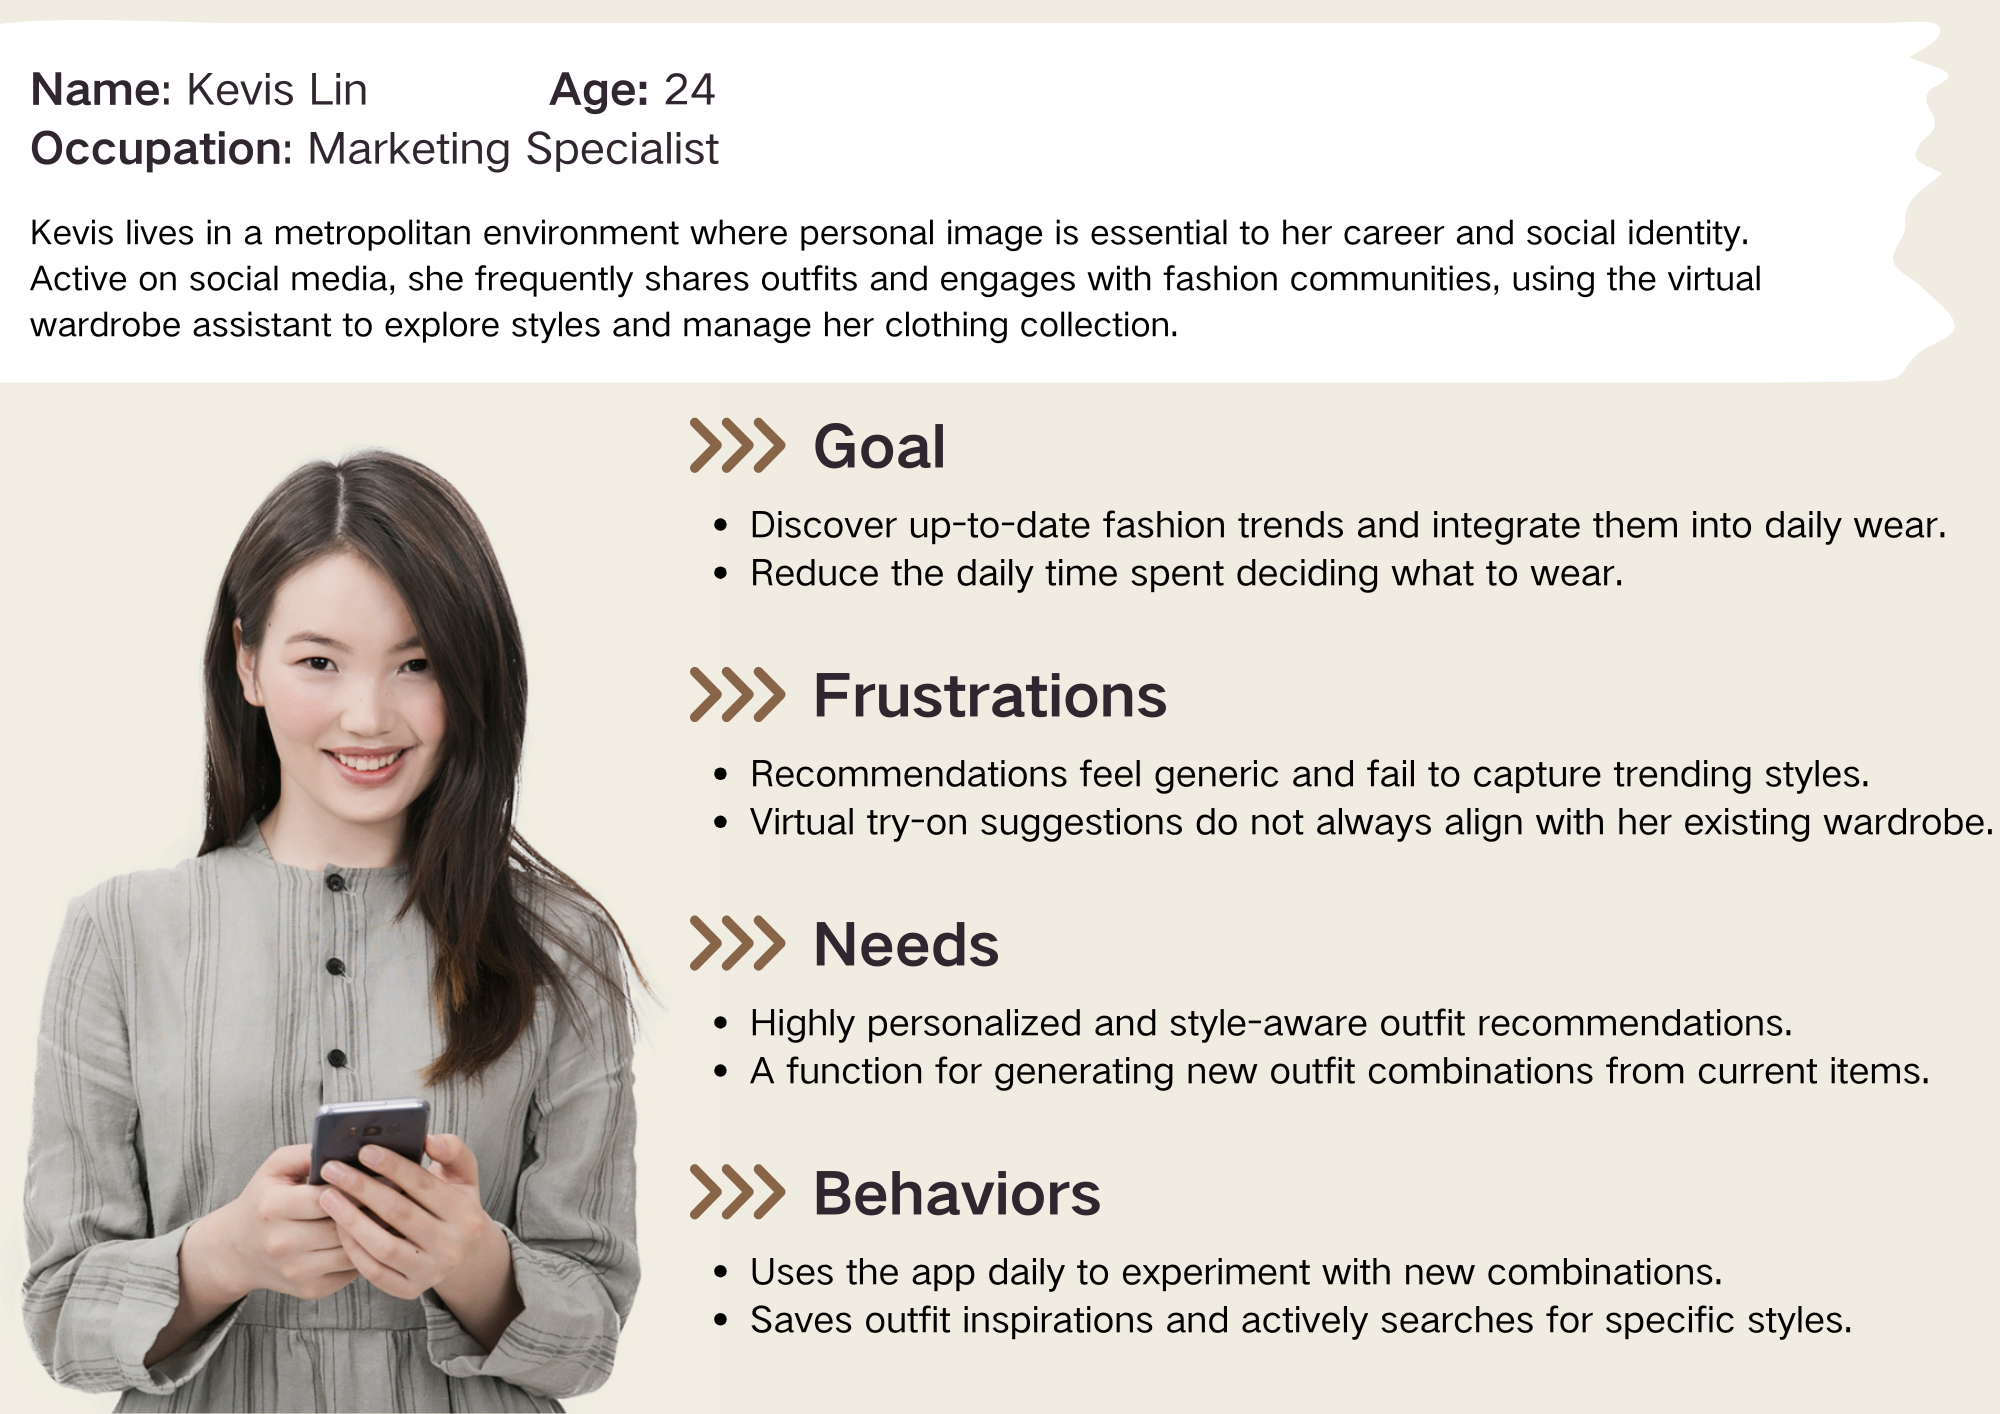
\includegraphics[width=0.80\textwidth]{images/Section_4_requirement/persona1.png}
    \caption{Fashion Explorer's persona}
    \label{fig:Kevis}
\end{figure}

Joe represents efficiency-focused users who want quick, reliable outfit decisions for professional settings. This persona is important because it highlights the need for weather-aware, occasion-appropriate recommendations and clear wardrobe organization. It directly supports the system requirements for weather-integrated recommendations and efficient wardrobe organization.

\begin{figure}[H]
    \centering
    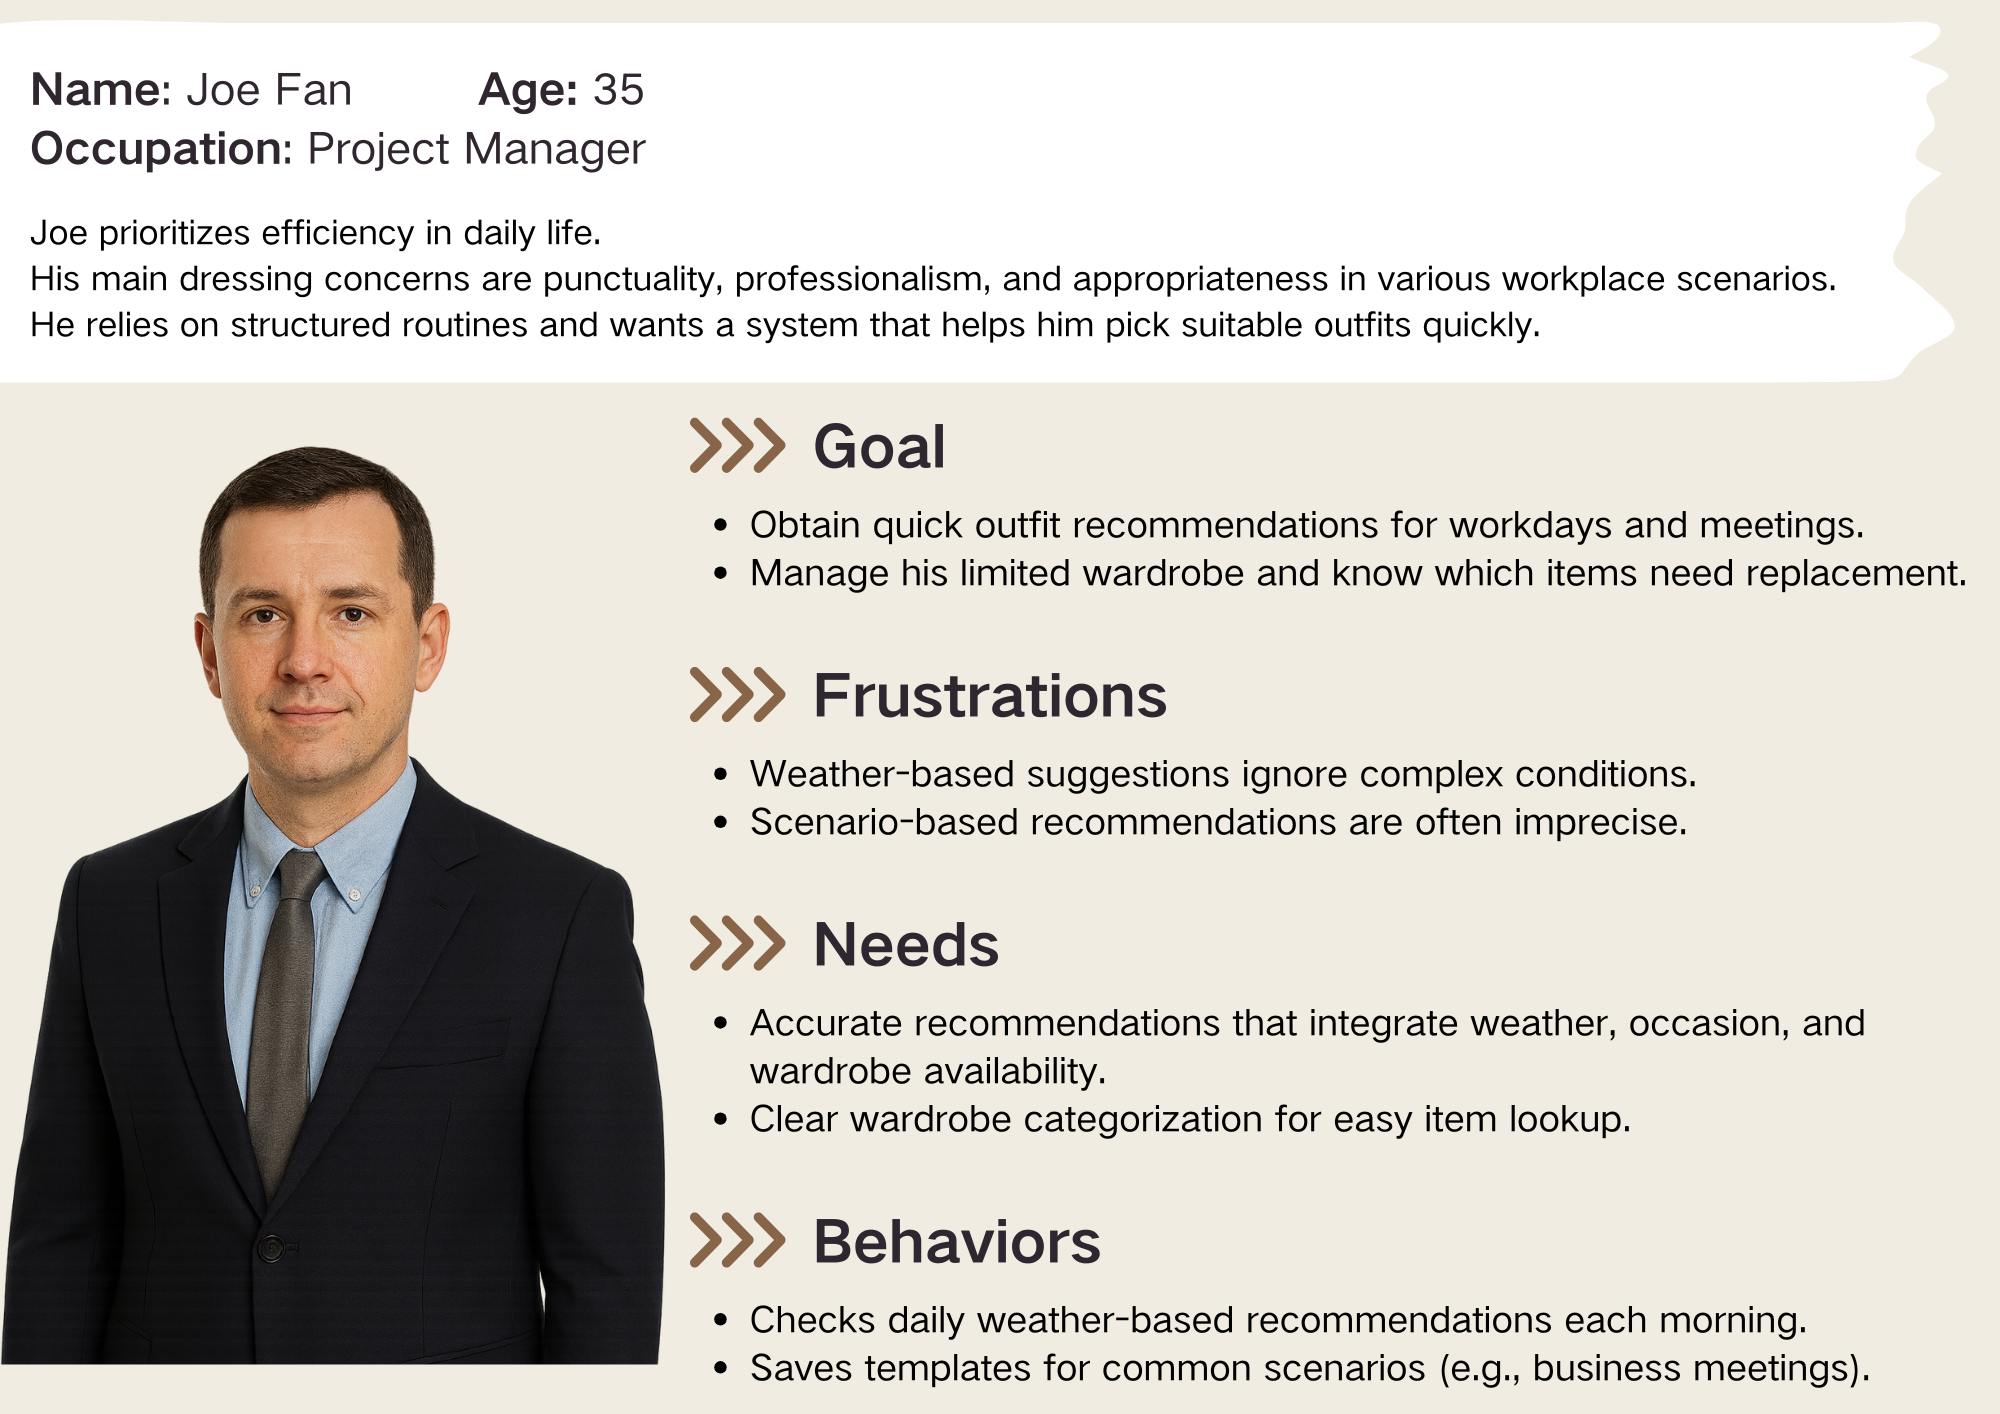
\includegraphics[width=0.80\textwidth]{images/Section_4_requirement/persona4.png}
    \caption{the Practicalist's persona}
    \label{fig:Joe}
\end{figure}

Jonathan represents the system-side stakeholder responsible for ensuring platform stability and user retention. This persona is important because his needs underscore the reliance on a scalable recommendation architecture and reliable performance. It directly supports key system requirements for model updates, data management, and continuous optimization.

\begin{figure}[H]
    \centering
    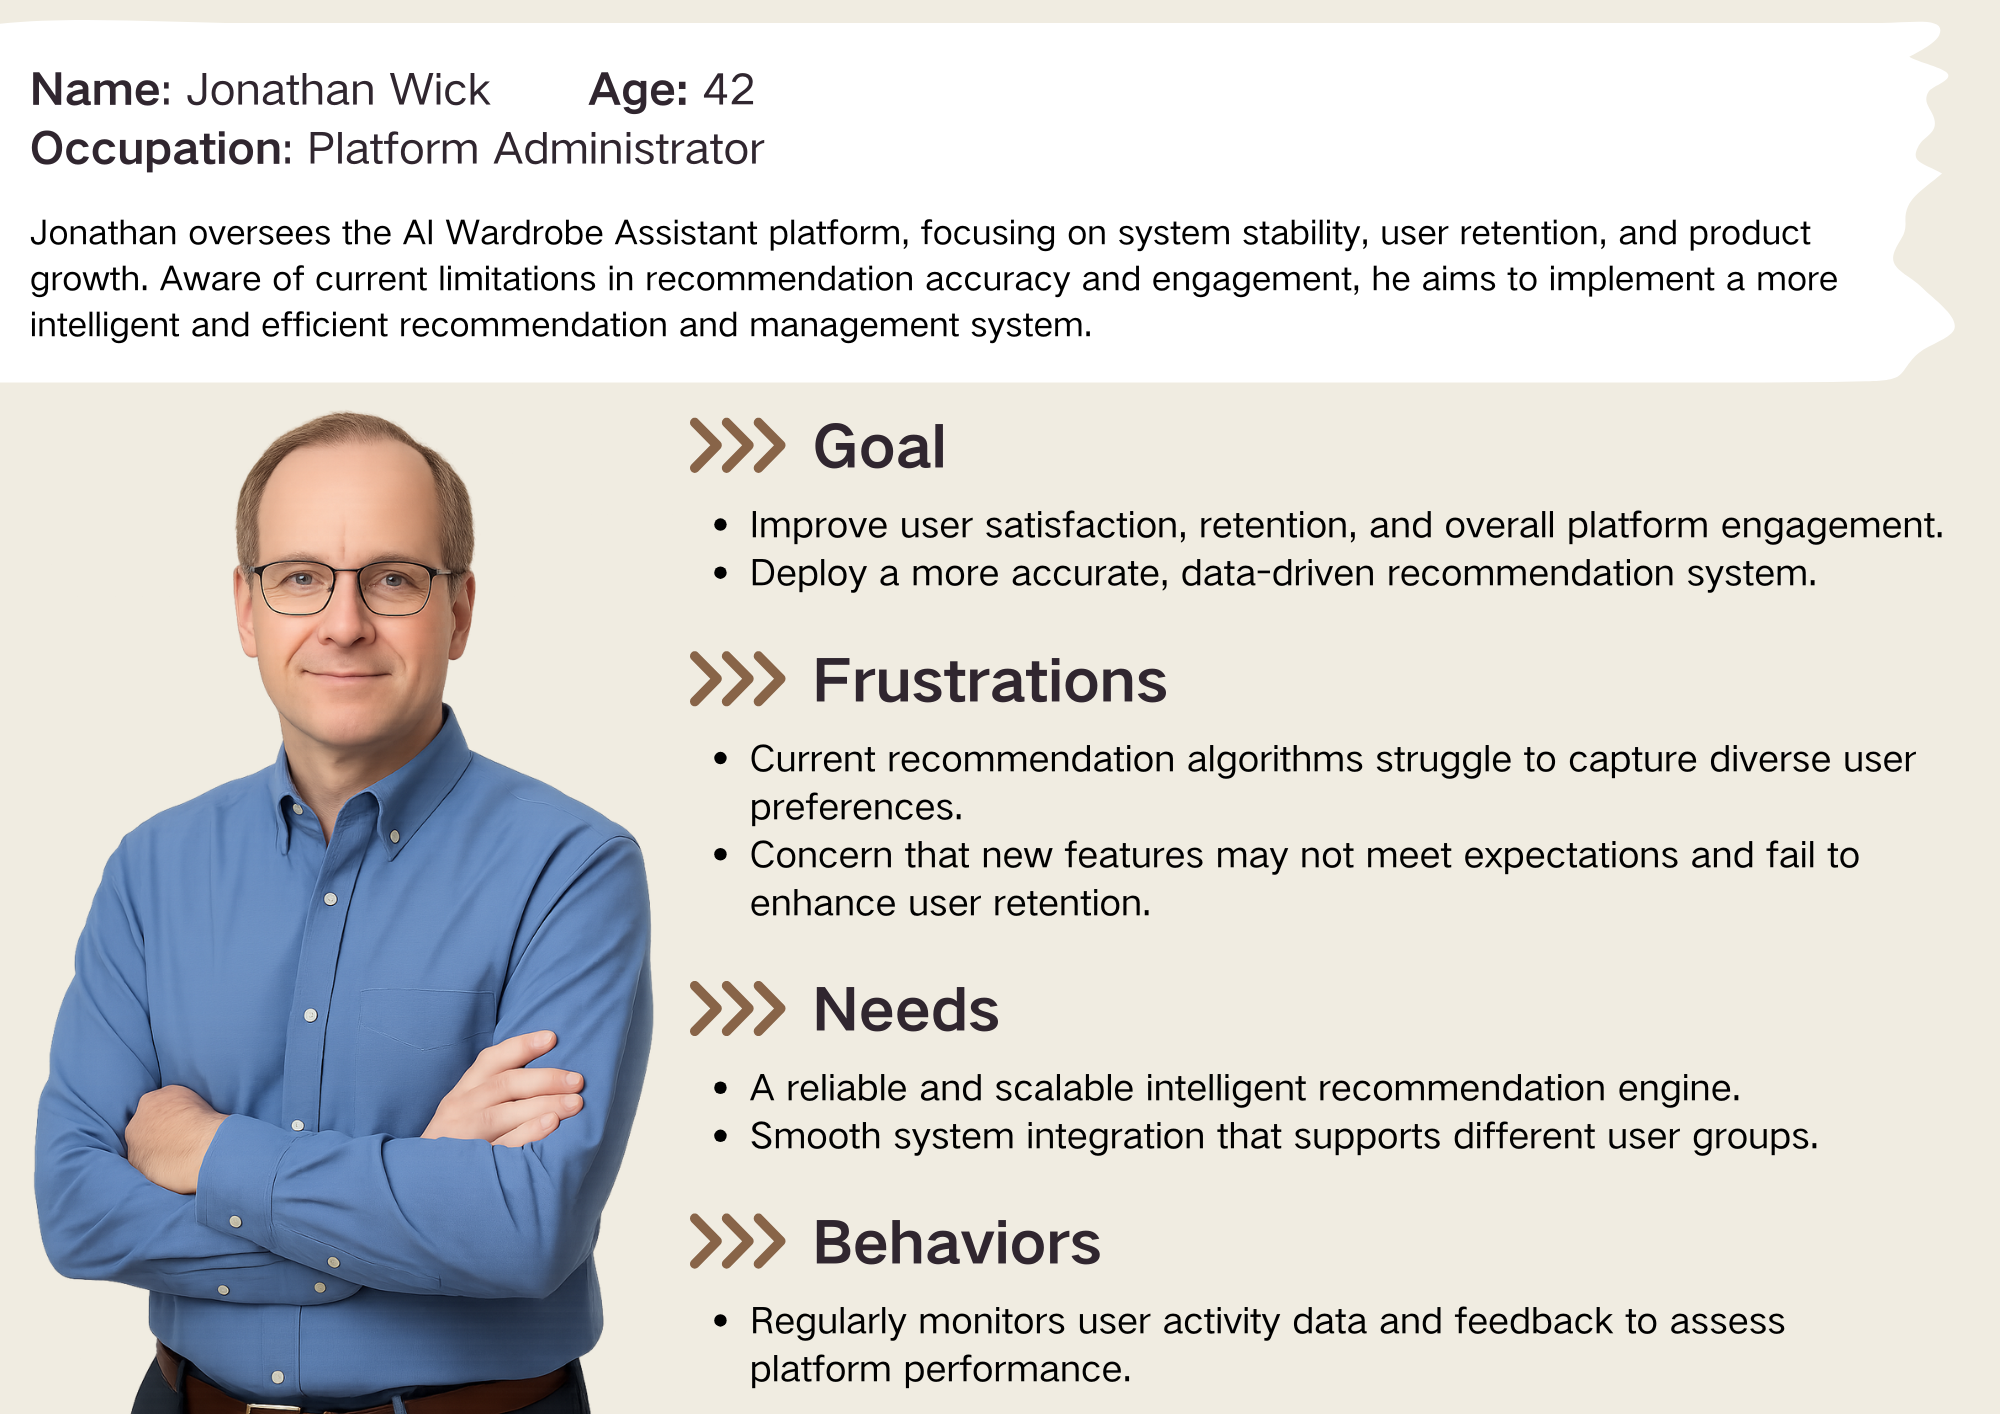
\includegraphics[width=0.80\textwidth]{images/Section_4_requirement/persona2.png}
    \caption{System Administrator's persona}
    \label{fig:Jonathan}
\end{figure}

Kiki represents users who prioritize practicality and reducing clothing waste. This persona is important because it highlights the need for style-compatible recommendations grounded in existing wardrobe items, as well as insights into usage patterns. It directly supports system requirements related to wardrobe analysis, outfit generation, and virtual try-on.

\begin{figure}[H]
    \centering
    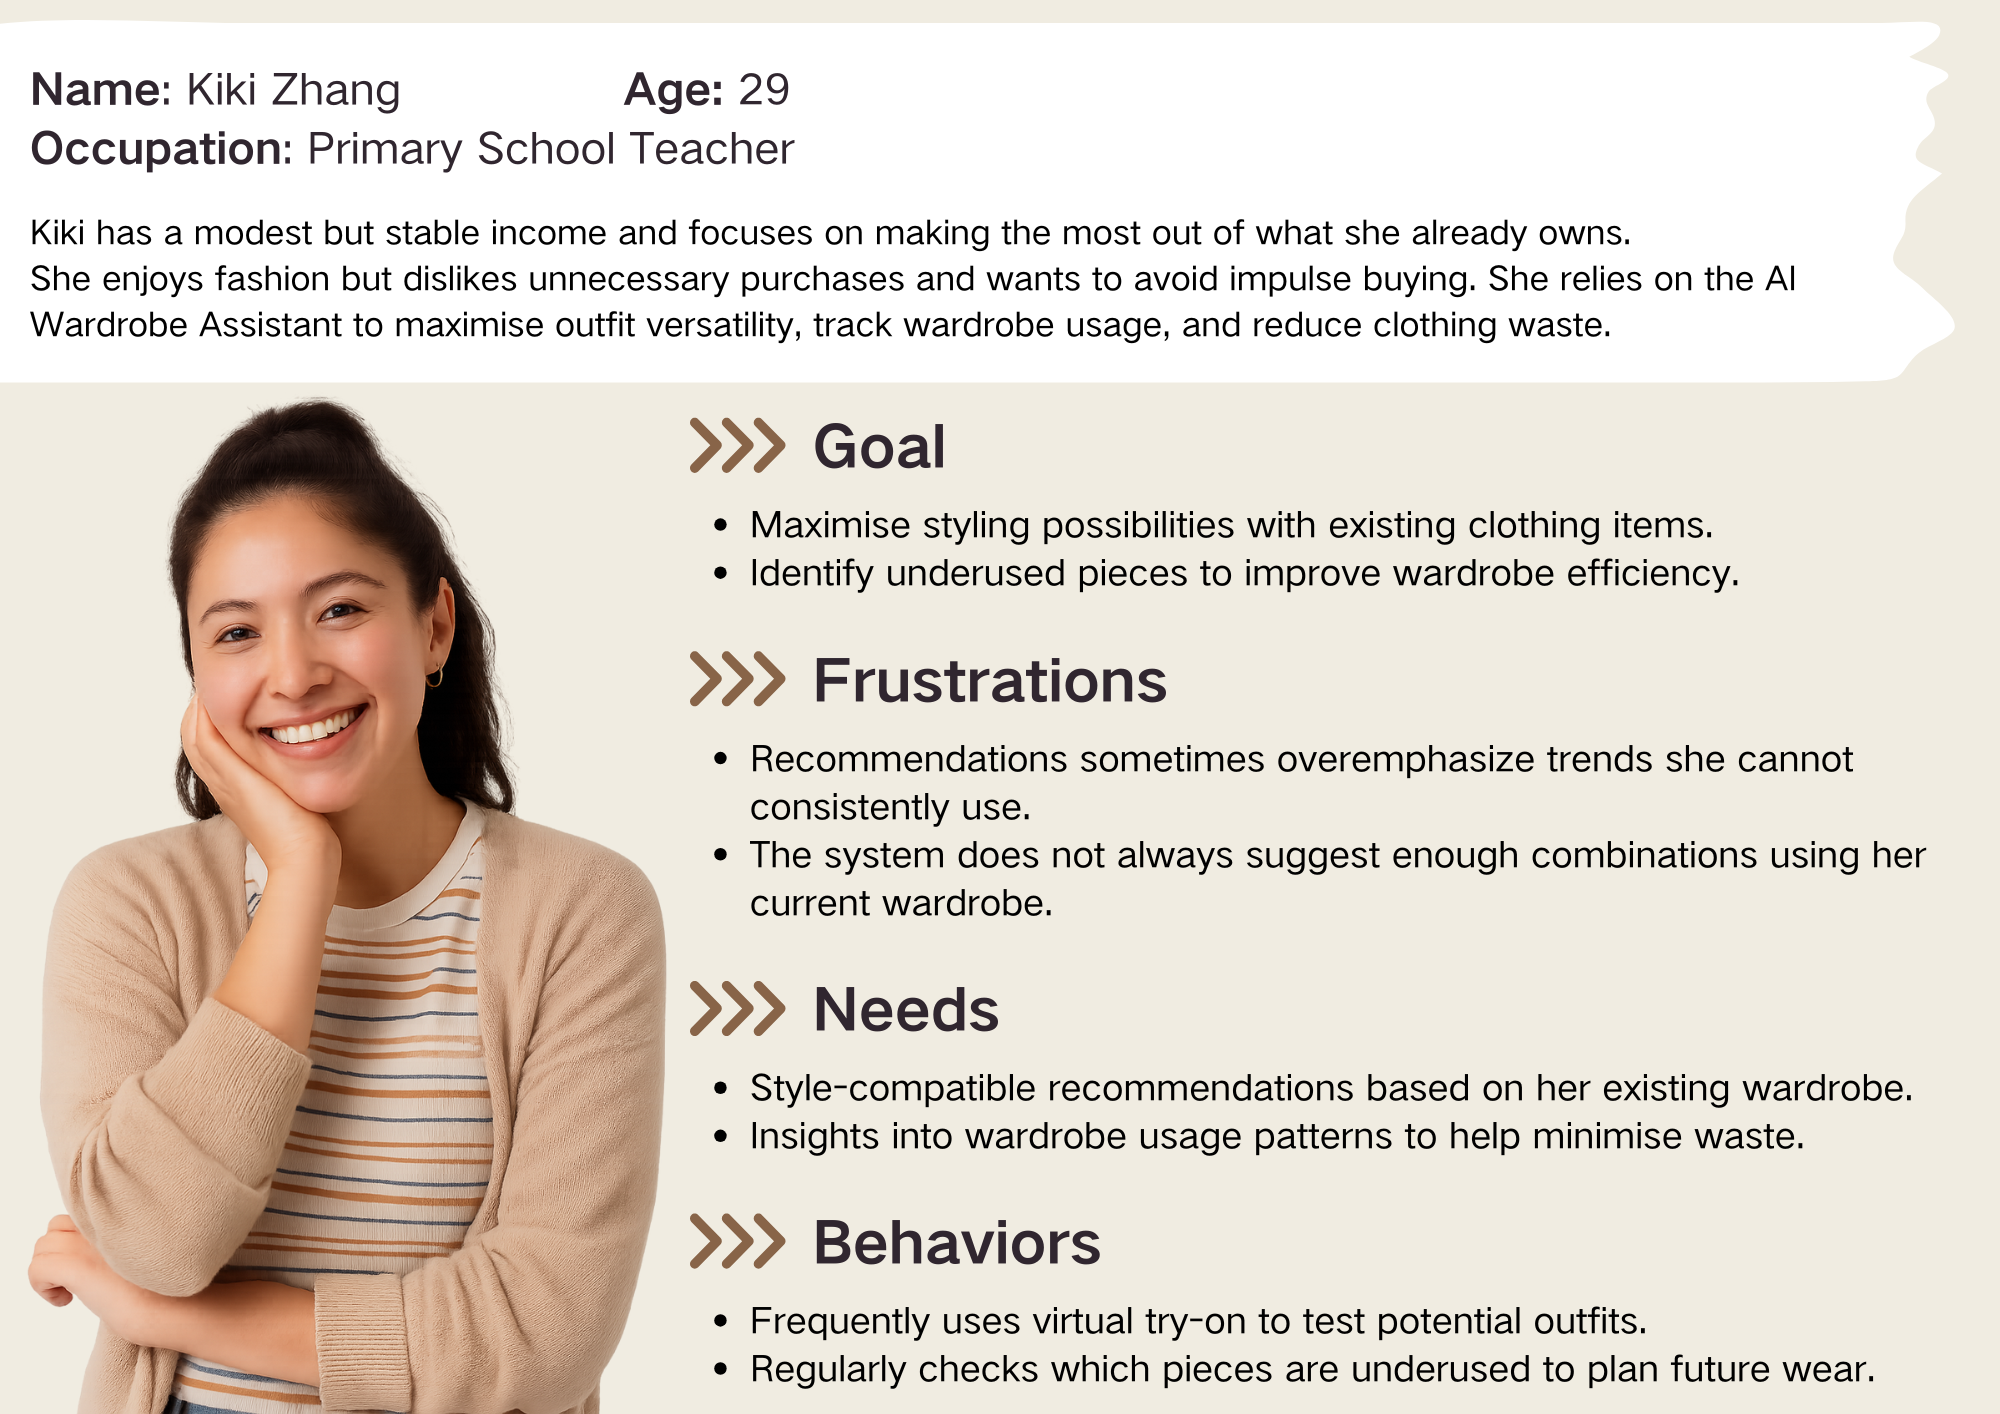
\includegraphics[width=0.80\textwidth]{images/Section_4_requirement/persona3.png}
    \caption{Wardrobe Optimizer's persona}
    \label{fig:Kiki}
\end{figure}


\section{User Story}

\textbf{\large 1. Kevis Lin — Fashion Explorer}\\

\textbf{US1.}\\
As a fashion enthusiast, I want personalized and trend-aware outfit recommendations so that I can remain stylish and express my unique identity.

\textbf{US2.}\\
As someone who frequently experiments with outfits, I want quick and relevant style suggestions so that I can reduce the time spent deciding what to wear each day.\\

\textbf{\large 2. Joe Fan — The Practicalist}\\

\textbf{US3.}\\
As a busy professional, I want one-click outfit suggestions based on weather and occasion so that I can dress appropriately with minimal effort.

\textbf{US4.}\\
As a wardrobe manager, I want my clothes clearly categorized in the app so that I can quickly find items.\\

\textbf{\large 3. Jonathan Wick — System Administrator}\\

\textbf{US5.}\\
As a data-driven operator, I want to analyze user behavior so that I can optimize future improvements.\\

\textbf{\large 4. Kiki Zhang — Wardrobe Optimizer}\\

\textbf{US6.}\\
As a wardrobe optimizer, I want guidance on styling items I already own so that I can maximize the value of my wardrobe.


\chapter{Qwen-Image-Edit Implementation Examples}
\label{appendix: Qwen}

\section{Additional Clothing and Accessories}

\begin{figure}[H]
    \centering
    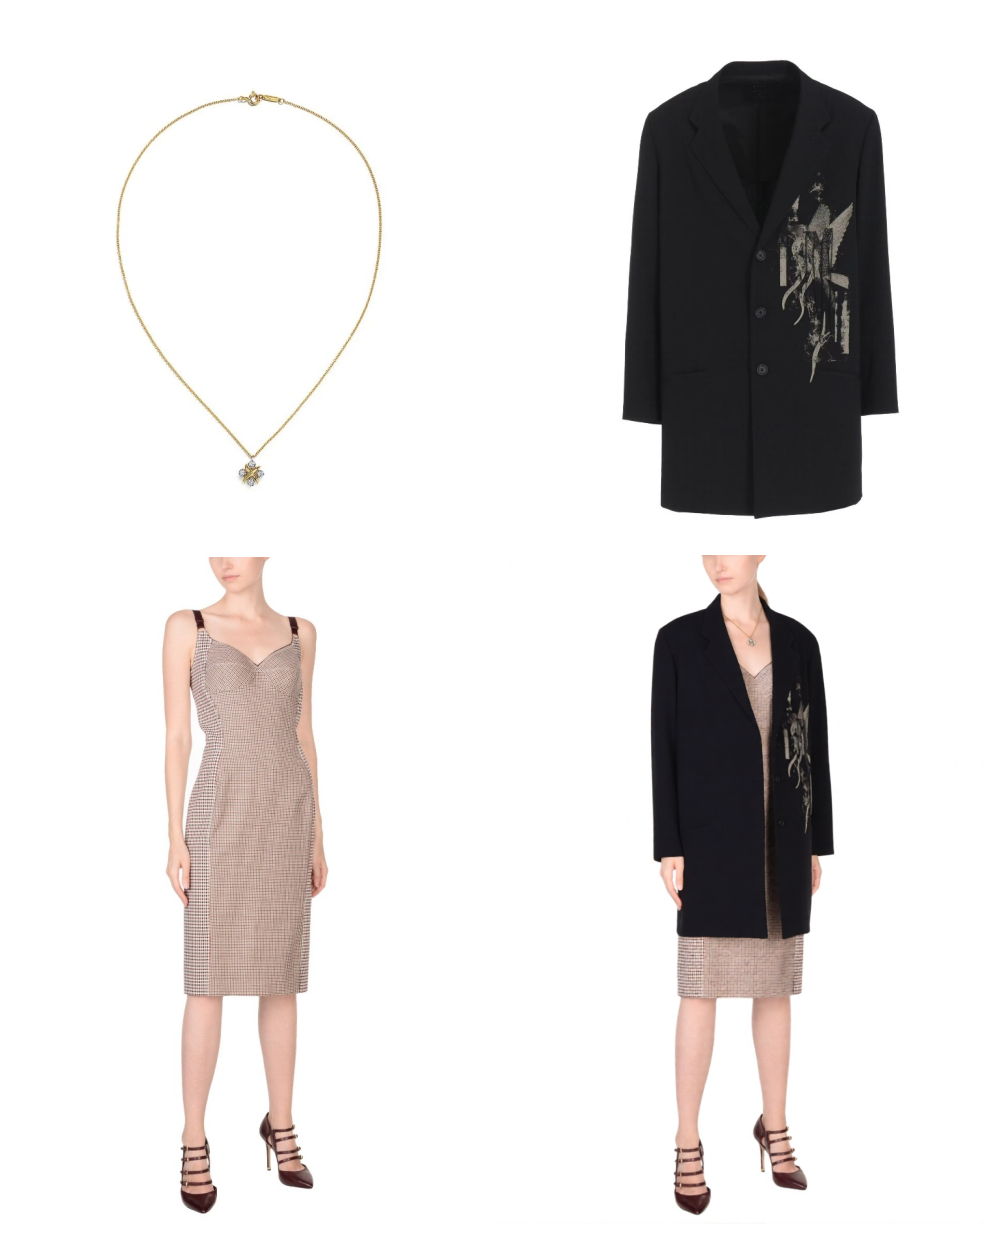
\includegraphics[width=0.6\textwidth]{images/Section_6.2.2/example1.png}
    \caption{Additional clothing and necklaces added to original outfit}
    \label{fig:example1}
\end{figure}

\noindent\textbf{Clarification for Figure~\ref{fig:example1}:}
\begin{itemize}
    \item Demonstrates the model's capability to add additional clothing items and accessories
    \item Shows realistic integration of necklaces with existing outfit
    \item Maintains consistency with original clothing style and fit
\end{itemize}

\section{Lower Body Virtual Fitting}

\begin{figure}[H]
    \centering
    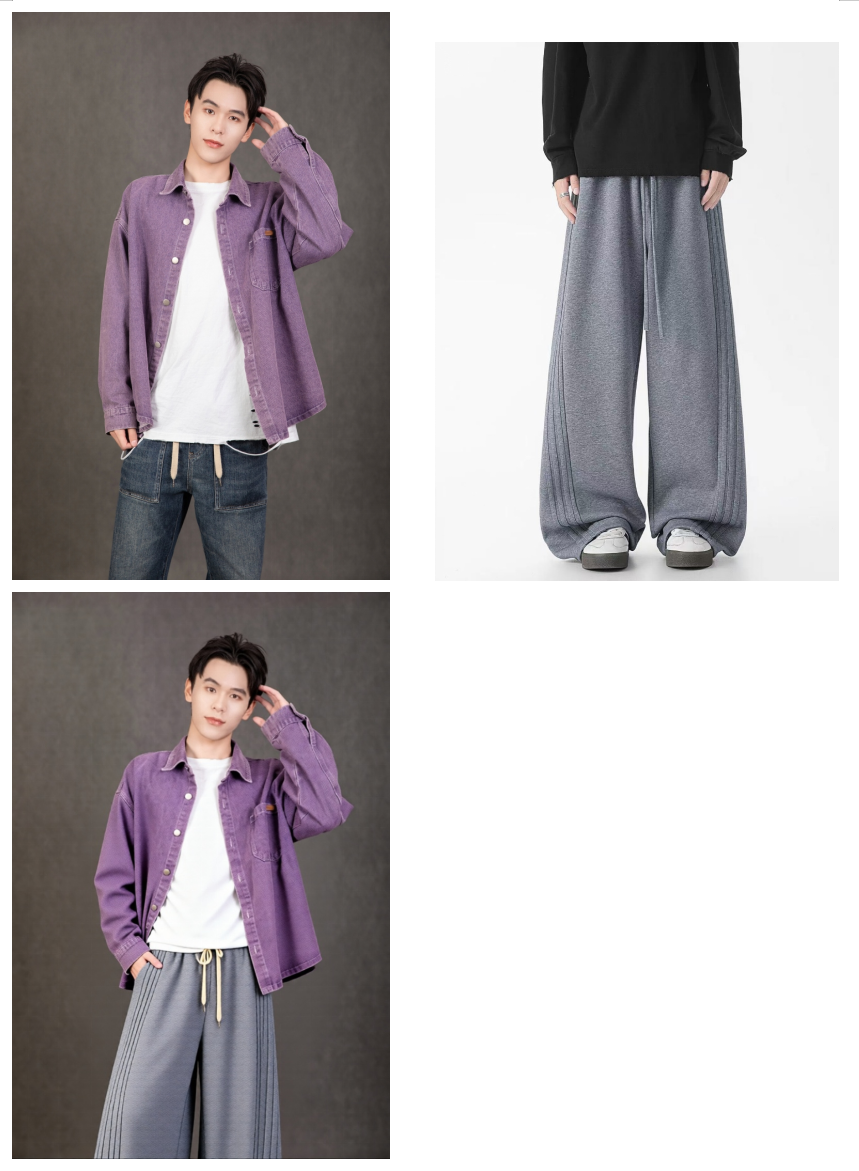
\includegraphics[width=0.6\textwidth]{images/Section_6.2.2/example2.png}
    \caption{Virtual fitting for the lower body}
    \label{fig:example2}
\end{figure}

\noindent\textbf{Clarification for Figure~\ref{fig:example2}:}
\begin{itemize}
    \item Specifically focuses on lower body clothing items
    \item Demonstrates accurate body shape adaptation
    \item Shows realistic fabric draping and fitting
\end{itemize}

\section{Jewelry Virtual Try-on}

\begin{figure}[H]
    \centering
    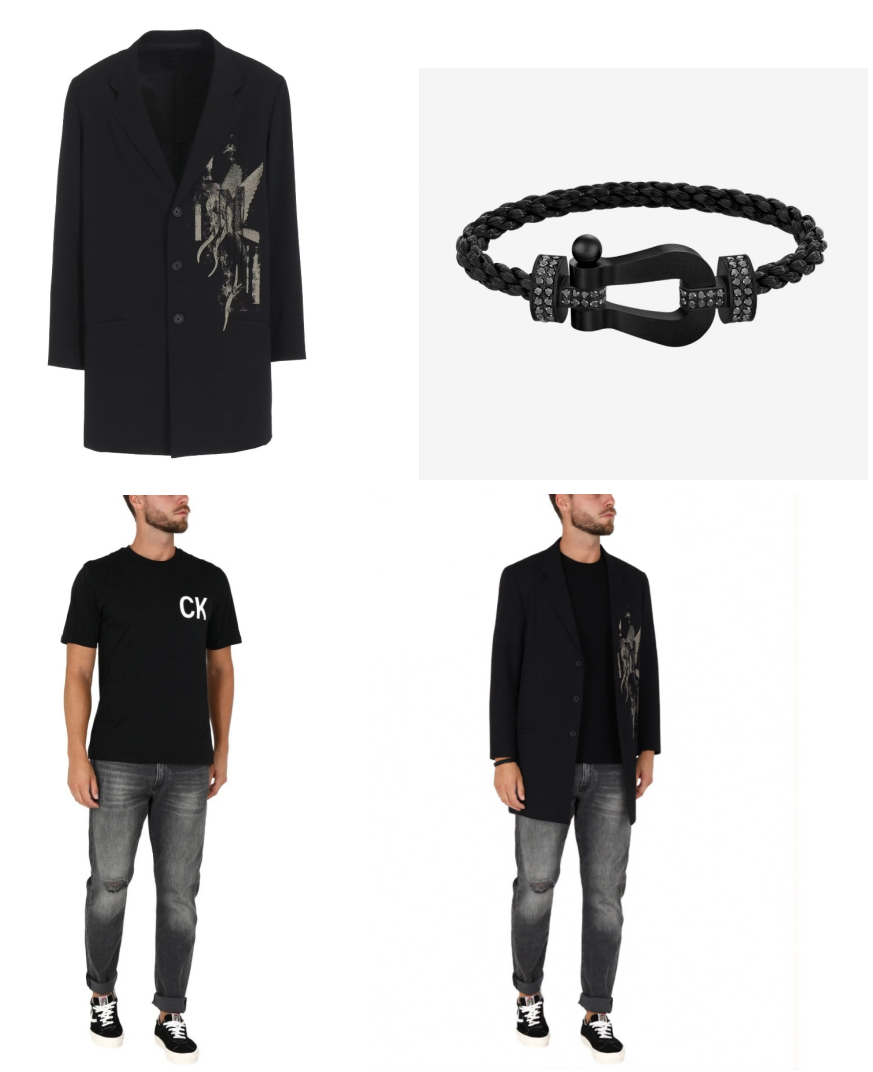
\includegraphics[width=0.6\textwidth]{images/Section_6.2.2/example3.png}
    \caption{Virtual try-on of jewelry}
    \label{fig:example3}
\end{figure}

\noindent\textbf{Clarification for Figure~\ref{fig:example3}:}
\begin{itemize}
    \item Illustrates precise jewelry positioning
    \item Shows realistic material representation
    \item Demonstrates natural integration with body features
\end{itemize}

\section{Earrings Virtual Fitting}

\begin{figure}[H]
    \centering
    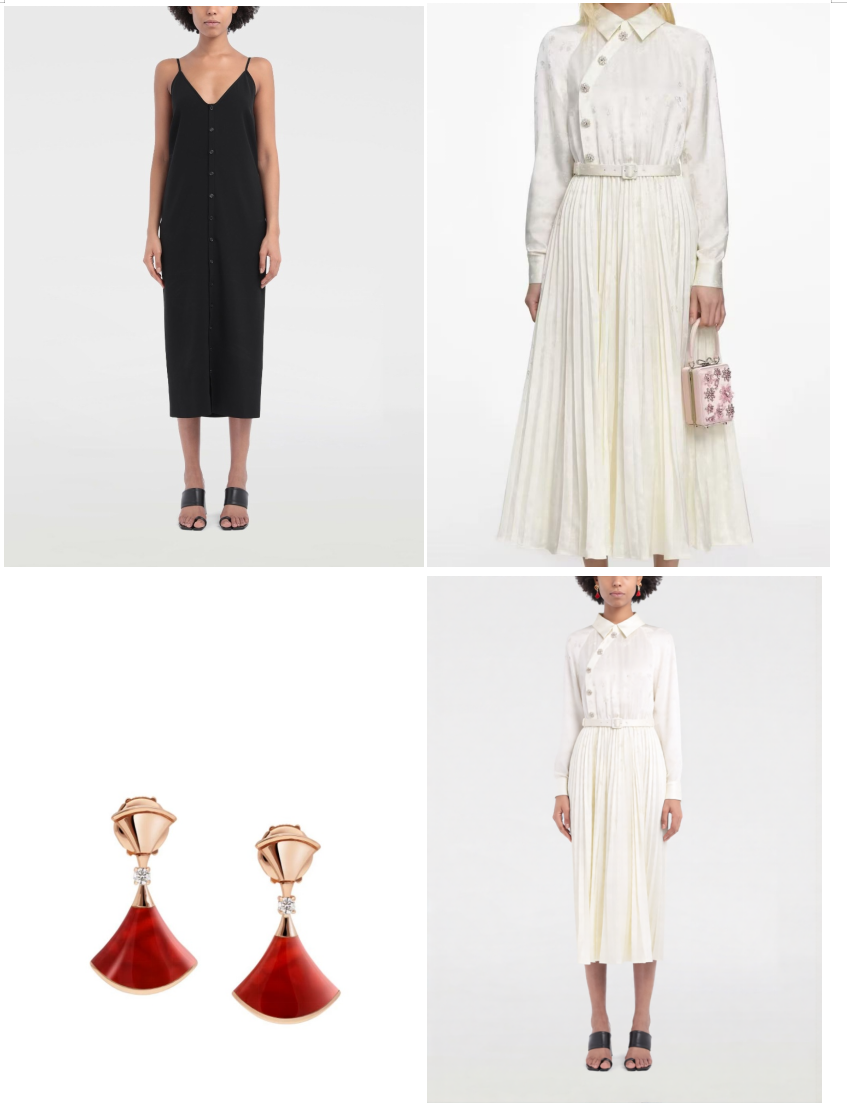
\includegraphics[width=0.6\textwidth]{images/Section_6.2.2/example4.png}
    \caption{Virtual fitting of earrings}
    \label{fig:example4}
\end{figure}

\noindent\textbf{Clarification for Figure~\ref{fig:example4}:}
\begin{itemize}
    \item Displays accurate earrings placement
    \item Shows attention to detail in accessory fitting
    \item Demonstrates natural integration with facial features 
\end{itemize}



\chapter{Detailed Database Architecture}
\label{database_schema}
\subsubsection{Users Table}
\begin{itemize}
    \item \texttt{id} (Primary Key, Integer) - Unique identifier for each user
    \item \texttt{username} (VARCHAR, Unique) - Unique username for login and profile identification
    \item \texttt{email} (VARCHAR, Unique) - Optional email address associated with the user
    \item \texttt{hashed\_password} (VARCHAR) - Encrypted password for authentication
    \item \texttt{is\_active} (Boolean) - Indicates whether the account is active
    \item \texttt{full\_name} (VARCHAR) - Optional full name of the user
    \item \texttt{avatar\_url} (VARCHAR) - Optional profile image URL
    \item \texttt{created\_at} (TIMESTAMP) - Account creation time
\end{itemize}

\subsubsection{Clothing Items Table}
\begin{itemize}
    \item \texttt{id} (Primary Key, Integer) - Unique identifier for each clothing item
    \item \texttt{user\_id} (Foreign Key) - References the owner user
    \item \texttt{name} (VARCHAR) - Name of the clothing item
    \item \texttt{image\_url} (VARCHAR) - URL of the clothing image
    \item \texttt{category} (ENUM) - Main clothing category
    \item \texttt{subcategory} (VARCHAR) - More specific clothing type
    \item \texttt{style} (VARCHAR) - Style description of the item
    \item \texttt{color} (VARCHAR) - Main color information
    \item \texttt{season} (ARRAY / ENUM) - Suitable seasons for the item
    \item \texttt{occasion} (VARCHAR) - Suitable wearing occasion
\end{itemize}

\subsubsection{Outfits Table}
\begin{itemize}
    \item \texttt{id} (Primary Key, Integer) - Unique identifier for each outfit
    \item \texttt{user\_id} (Foreign Key) - References the owner user
    \item \texttt{name} (VARCHAR) - Name of the outfit
    \item \texttt{description} (TEXT) - Text description of the outfit
    \item \texttt{occasion} (VARCHAR) - Target occasion for the outfit
    \item \texttt{season} (VARCHAR) - Suitable season for the outfit
    \item \texttt{style} (VARCHAR) - Overall style of the outfit
    \item \texttt{rating} (Integer) - User rating of the outfit
    \item \texttt{wear\_count} (Integer) - Number of times the outfit has been worn
    \item \texttt{created\_at} (TIMESTAMP) - Outfit creation time
\end{itemize}

\subsubsection{Wear History Table}
\begin{itemize}
    \item \texttt{id} (Primary Key, Integer) - Unique identifier for each wear record
    \item \texttt{user\_id} (Foreign Key) - References the related user
    \item \texttt{clothing\_id} (Foreign Key, Nullable) - References a worn clothing item
    \item \texttt{outfit\_id} (Foreign Key, Nullable) - References a worn outfit
    \item \texttt{wear\_date} (DATE) - Date of wearing
    \item \texttt{weather} (VARCHAR) - Weather information for the record
    \item \texttt{temperature} (Integer) - Temperature at the time of wearing
    \item \texttt{occasion} (VARCHAR) - Occasion associated with the wearing event
    \item \texttt{rating} (Integer) - User rating for the wearing experience
\end{itemize}

\subsubsection{Model Photos Table}
\begin{itemize}
    \item \texttt{id} (Primary Key, Integer) - Unique identifier for each model photo
    \item \texttt{user\_id} (Foreign Key) - References the owner user
    \item \texttt{photo\_name} (VARCHAR) - Name of the model photo
    \item \texttt{image\_url} (VARCHAR) - URL of the original photo
    \item \texttt{thumbnail\_url} (VARCHAR) - URL of the thumbnail image
    \item \texttt{file\_format} (VARCHAR) - File format such as jpg or png
    \item \texttt{is\_active} (Boolean) - Indicates whether the photo is active
    \item \texttt{is\_primary} (Boolean) - Indicates whether the photo is the default model image
\end{itemize}

\subsubsection{AI Conversations Table}
\begin{itemize}
    \item \texttt{id} (Primary Key, Integer) - Unique identifier for each conversation
    \item \texttt{user\_id} (Foreign Key) - References the related user
    \item \texttt{title} (VARCHAR) - Conversation title
    \item \texttt{messages} (JSON) - Stored message list in structured format
    \item \texttt{created\_at} (TIMESTAMP) - Conversation creation time
    \item \texttt{updated\_at} (TIMESTAMP) - Last update time of the conversation
\end{itemize}



\chapter{Formal Meeting Minutes}
\section{1st Formal Meeting Minutes (2025-10-17)}
\begin{figure}[H]
    \centering
    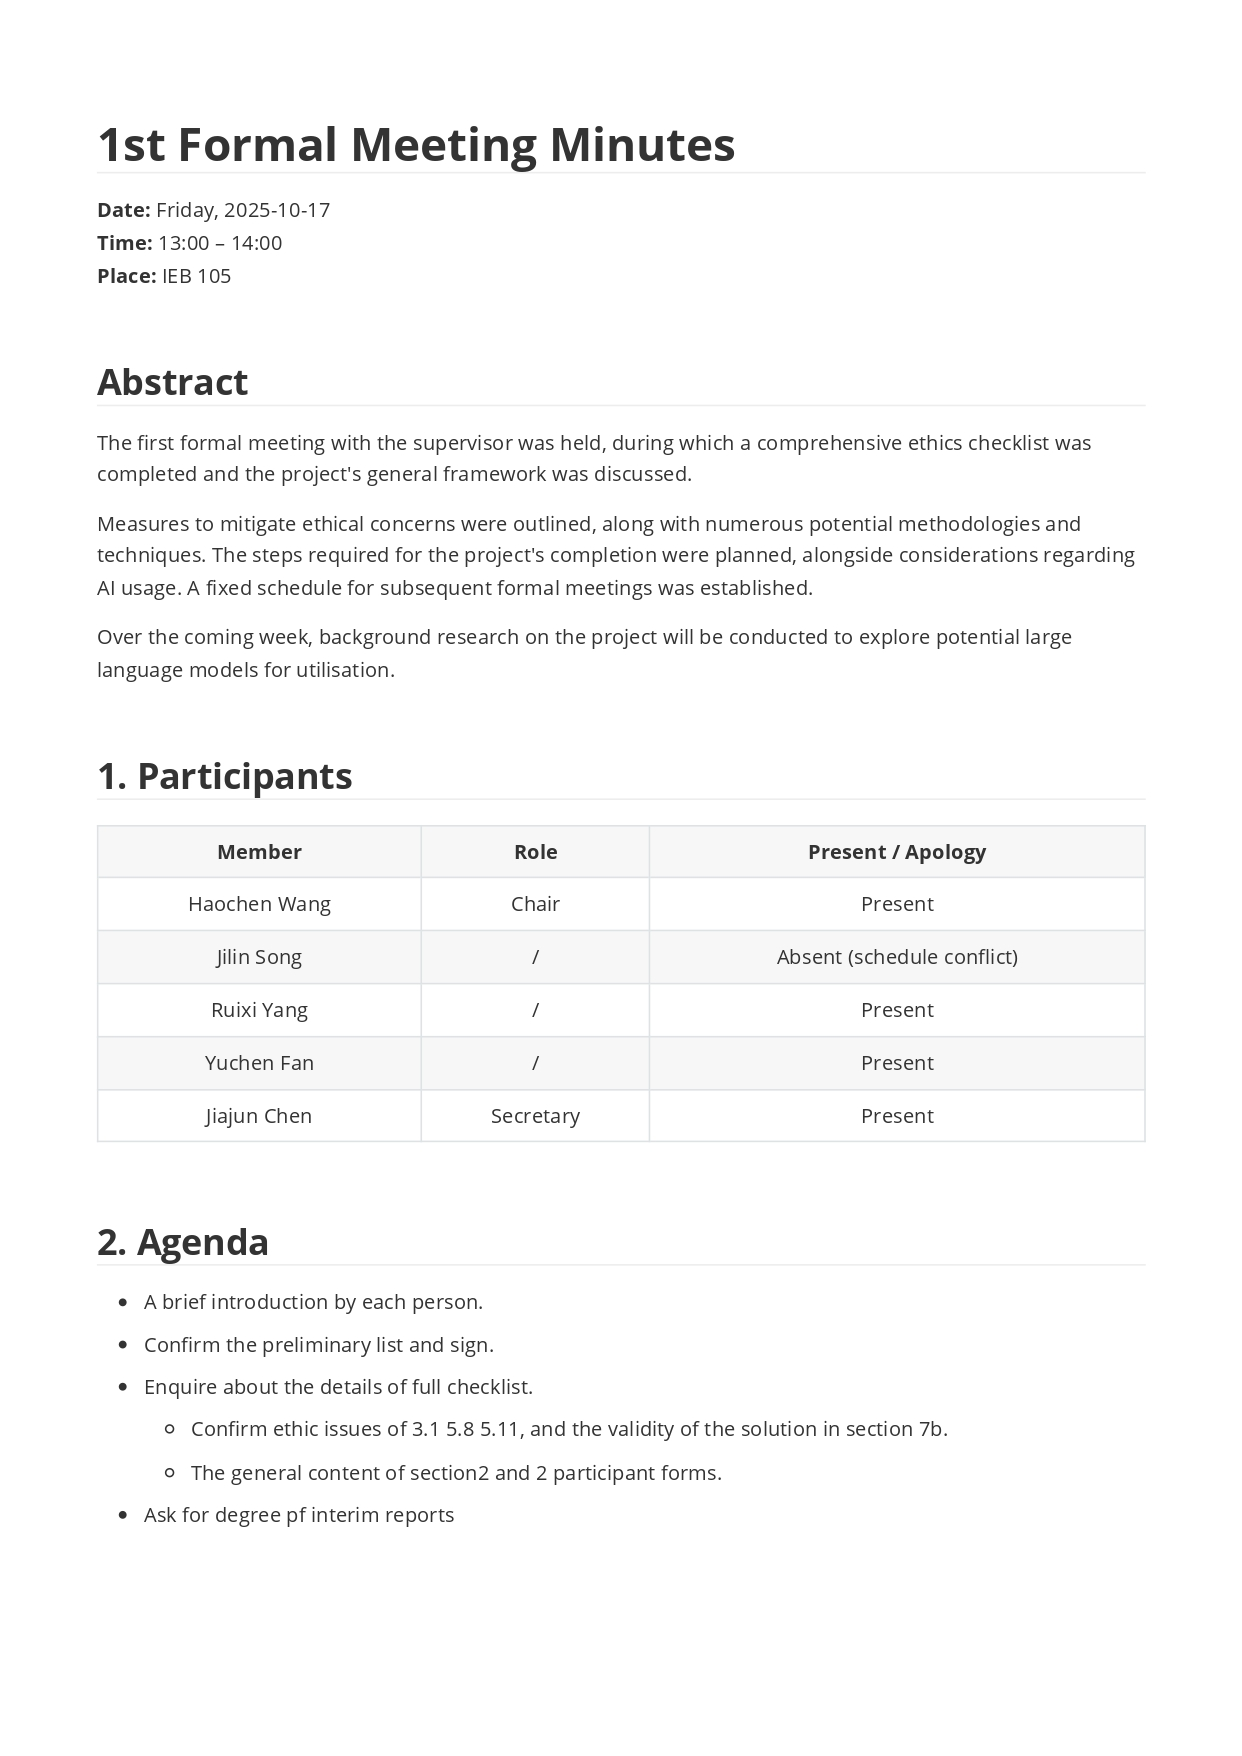
\includegraphics[width=0.8\textwidth]{images/appendix/1st_Formal_Meeting_Minutes_2025-10-17_page-0001.jpg}
\end{figure}
\begin{figure}[H]
    \centering
    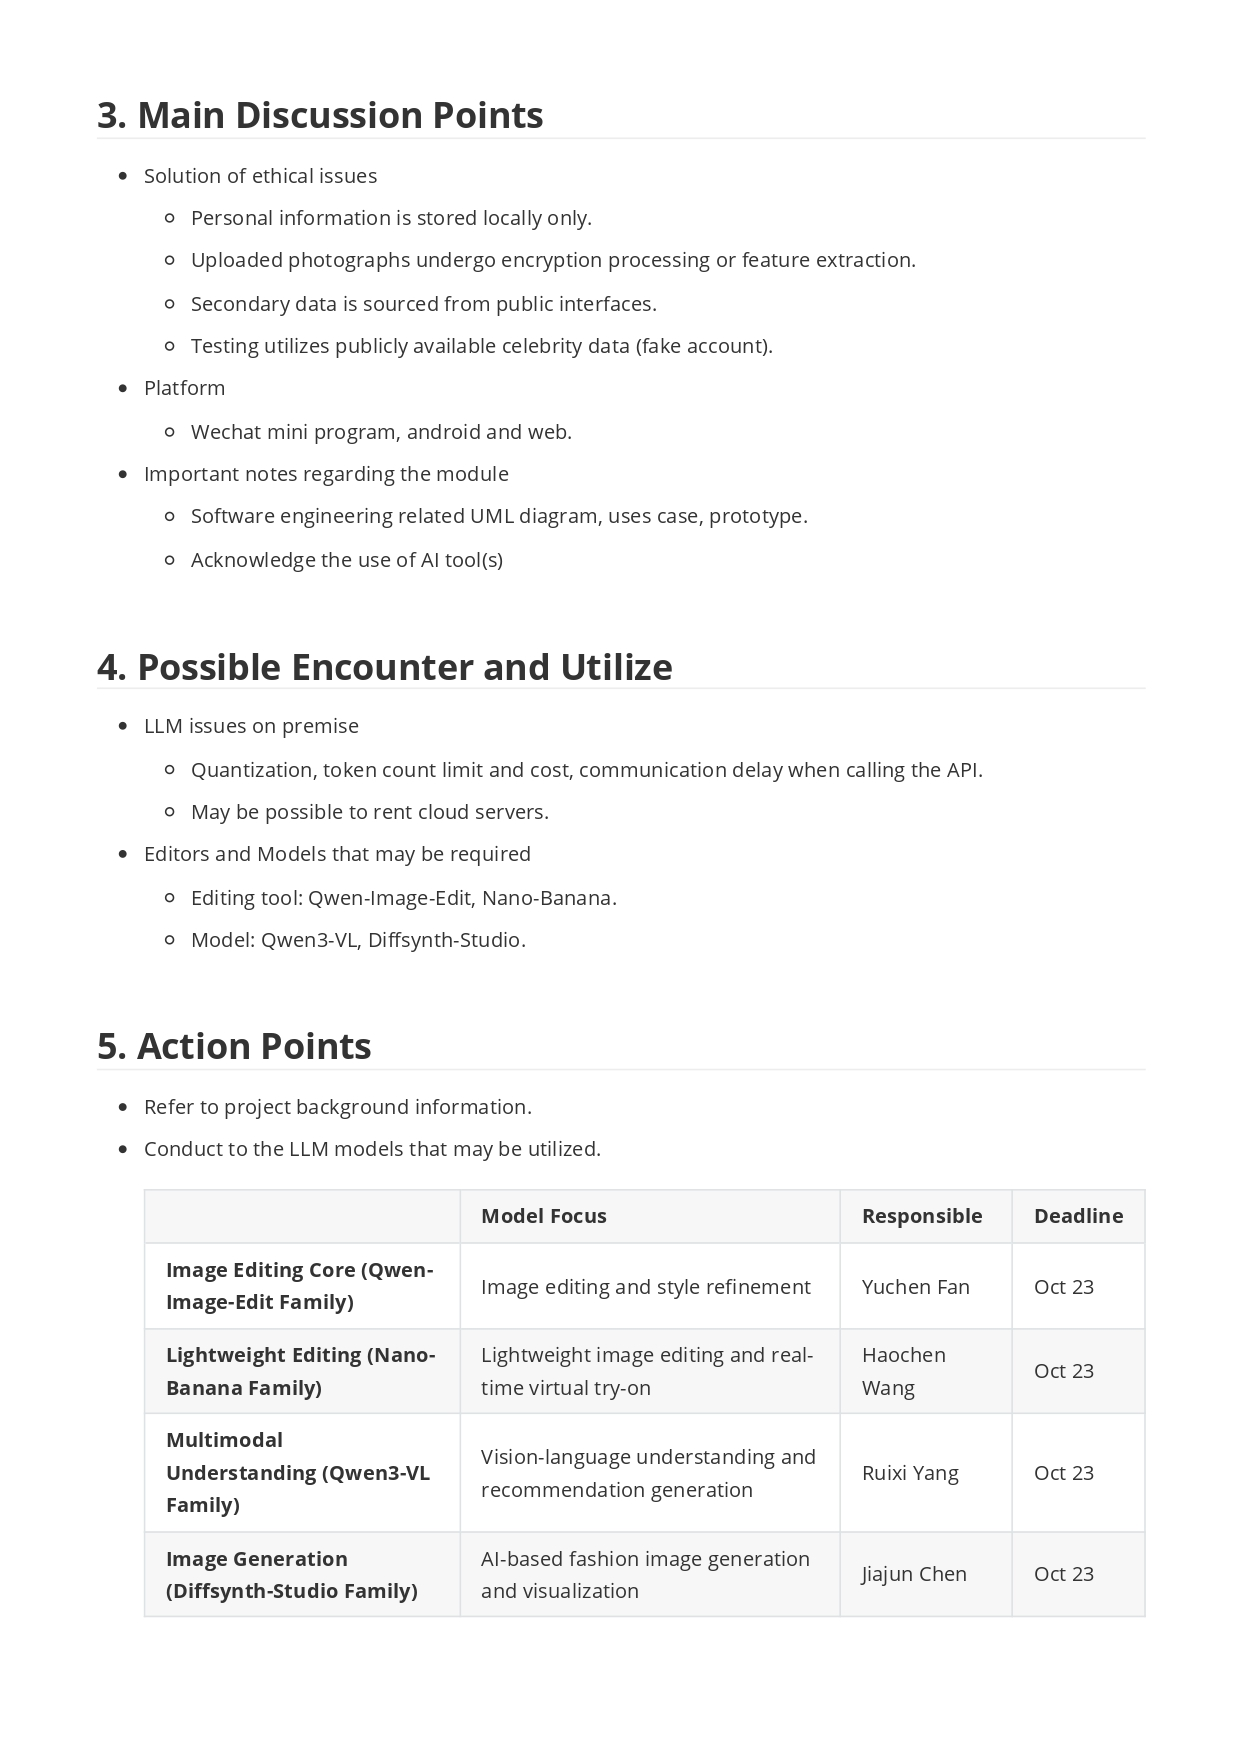
\includegraphics[width=1.0\textwidth]{images/appendix/1st_Formal_Meeting_Minutes_2025-10-17_page-0002.jpg}
\end{figure}
\begin{figure}[H]
    \centering
    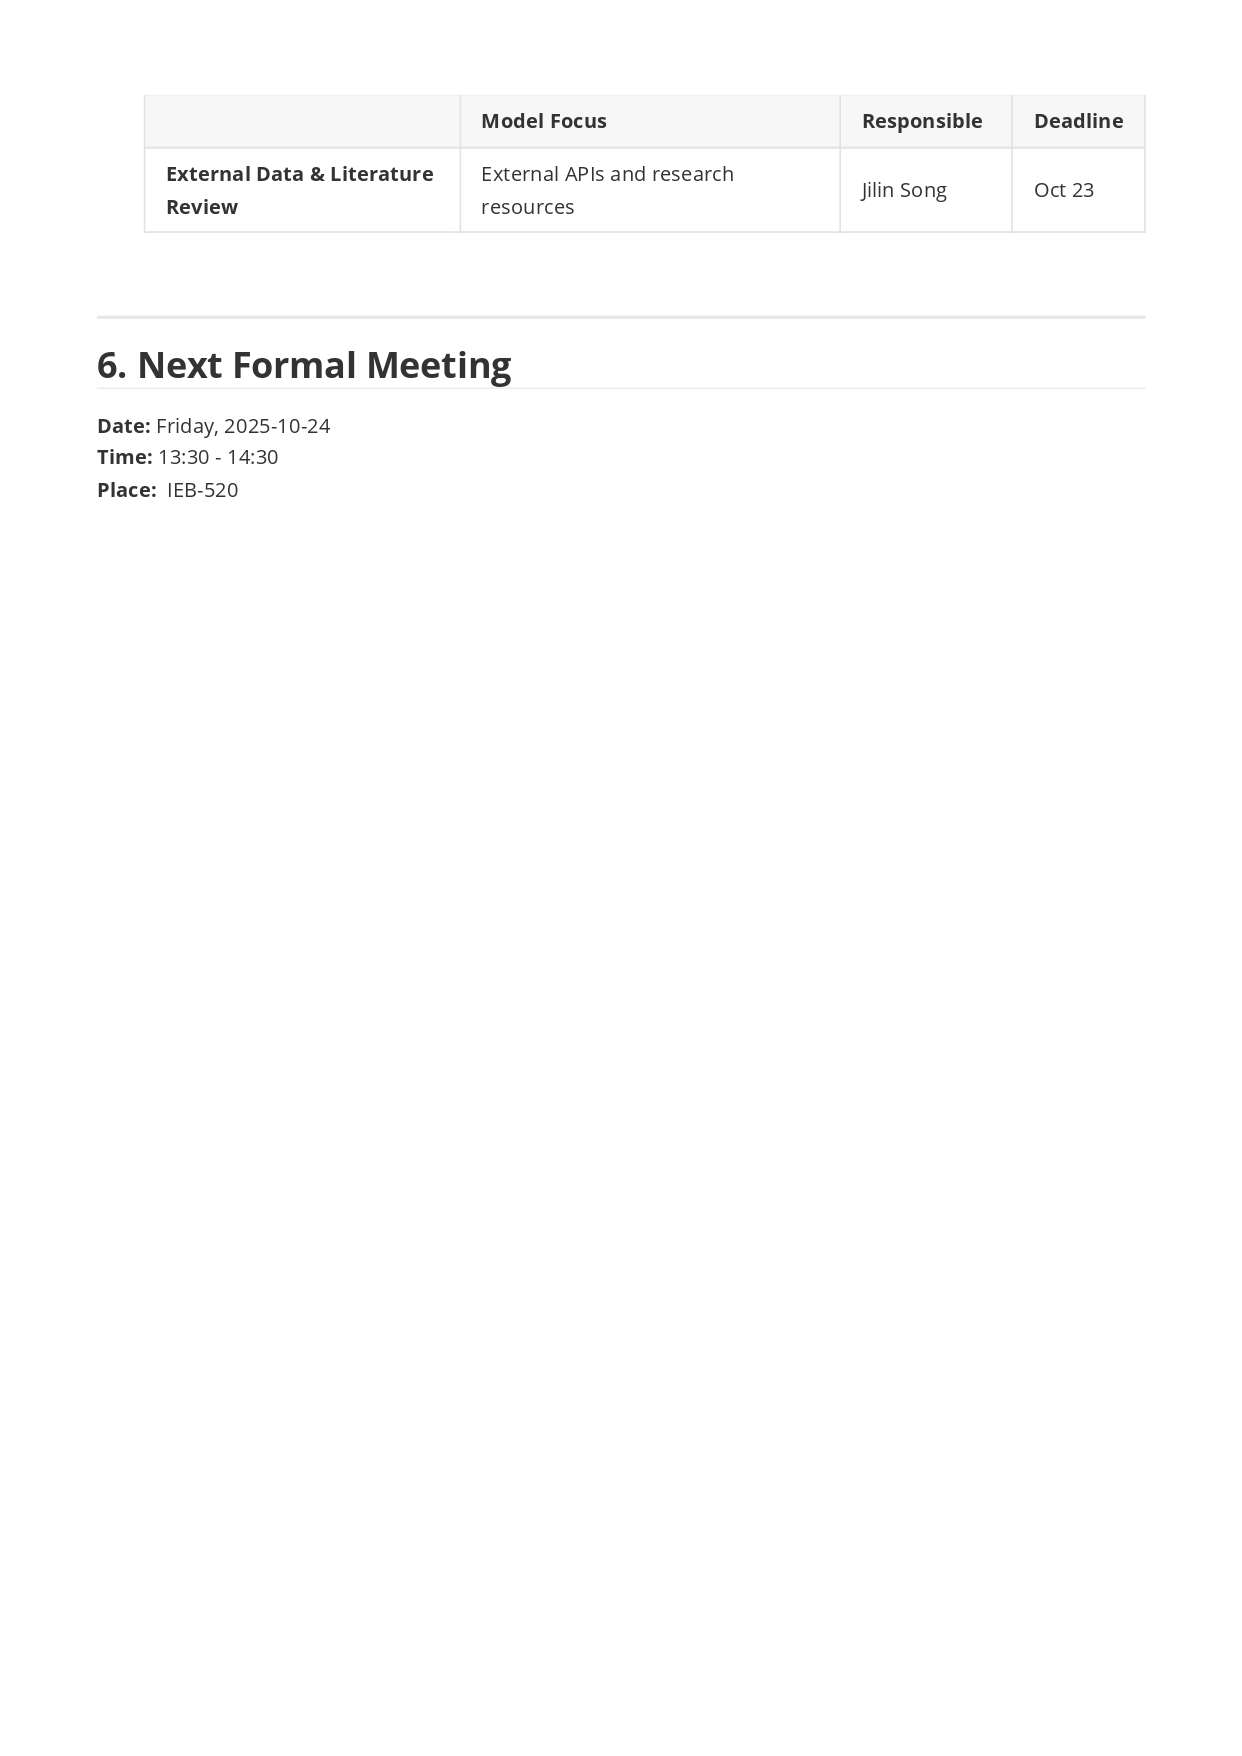
\includegraphics[width=1.0\textwidth]{images/appendix/1st_Formal_Meeting_Minutes_2025-10-17_page-0003.jpg}
\end{figure}


\section{1st Informal Meeting Minutes (2025-10-16)}
\begin{figure}[H]
    \centering
    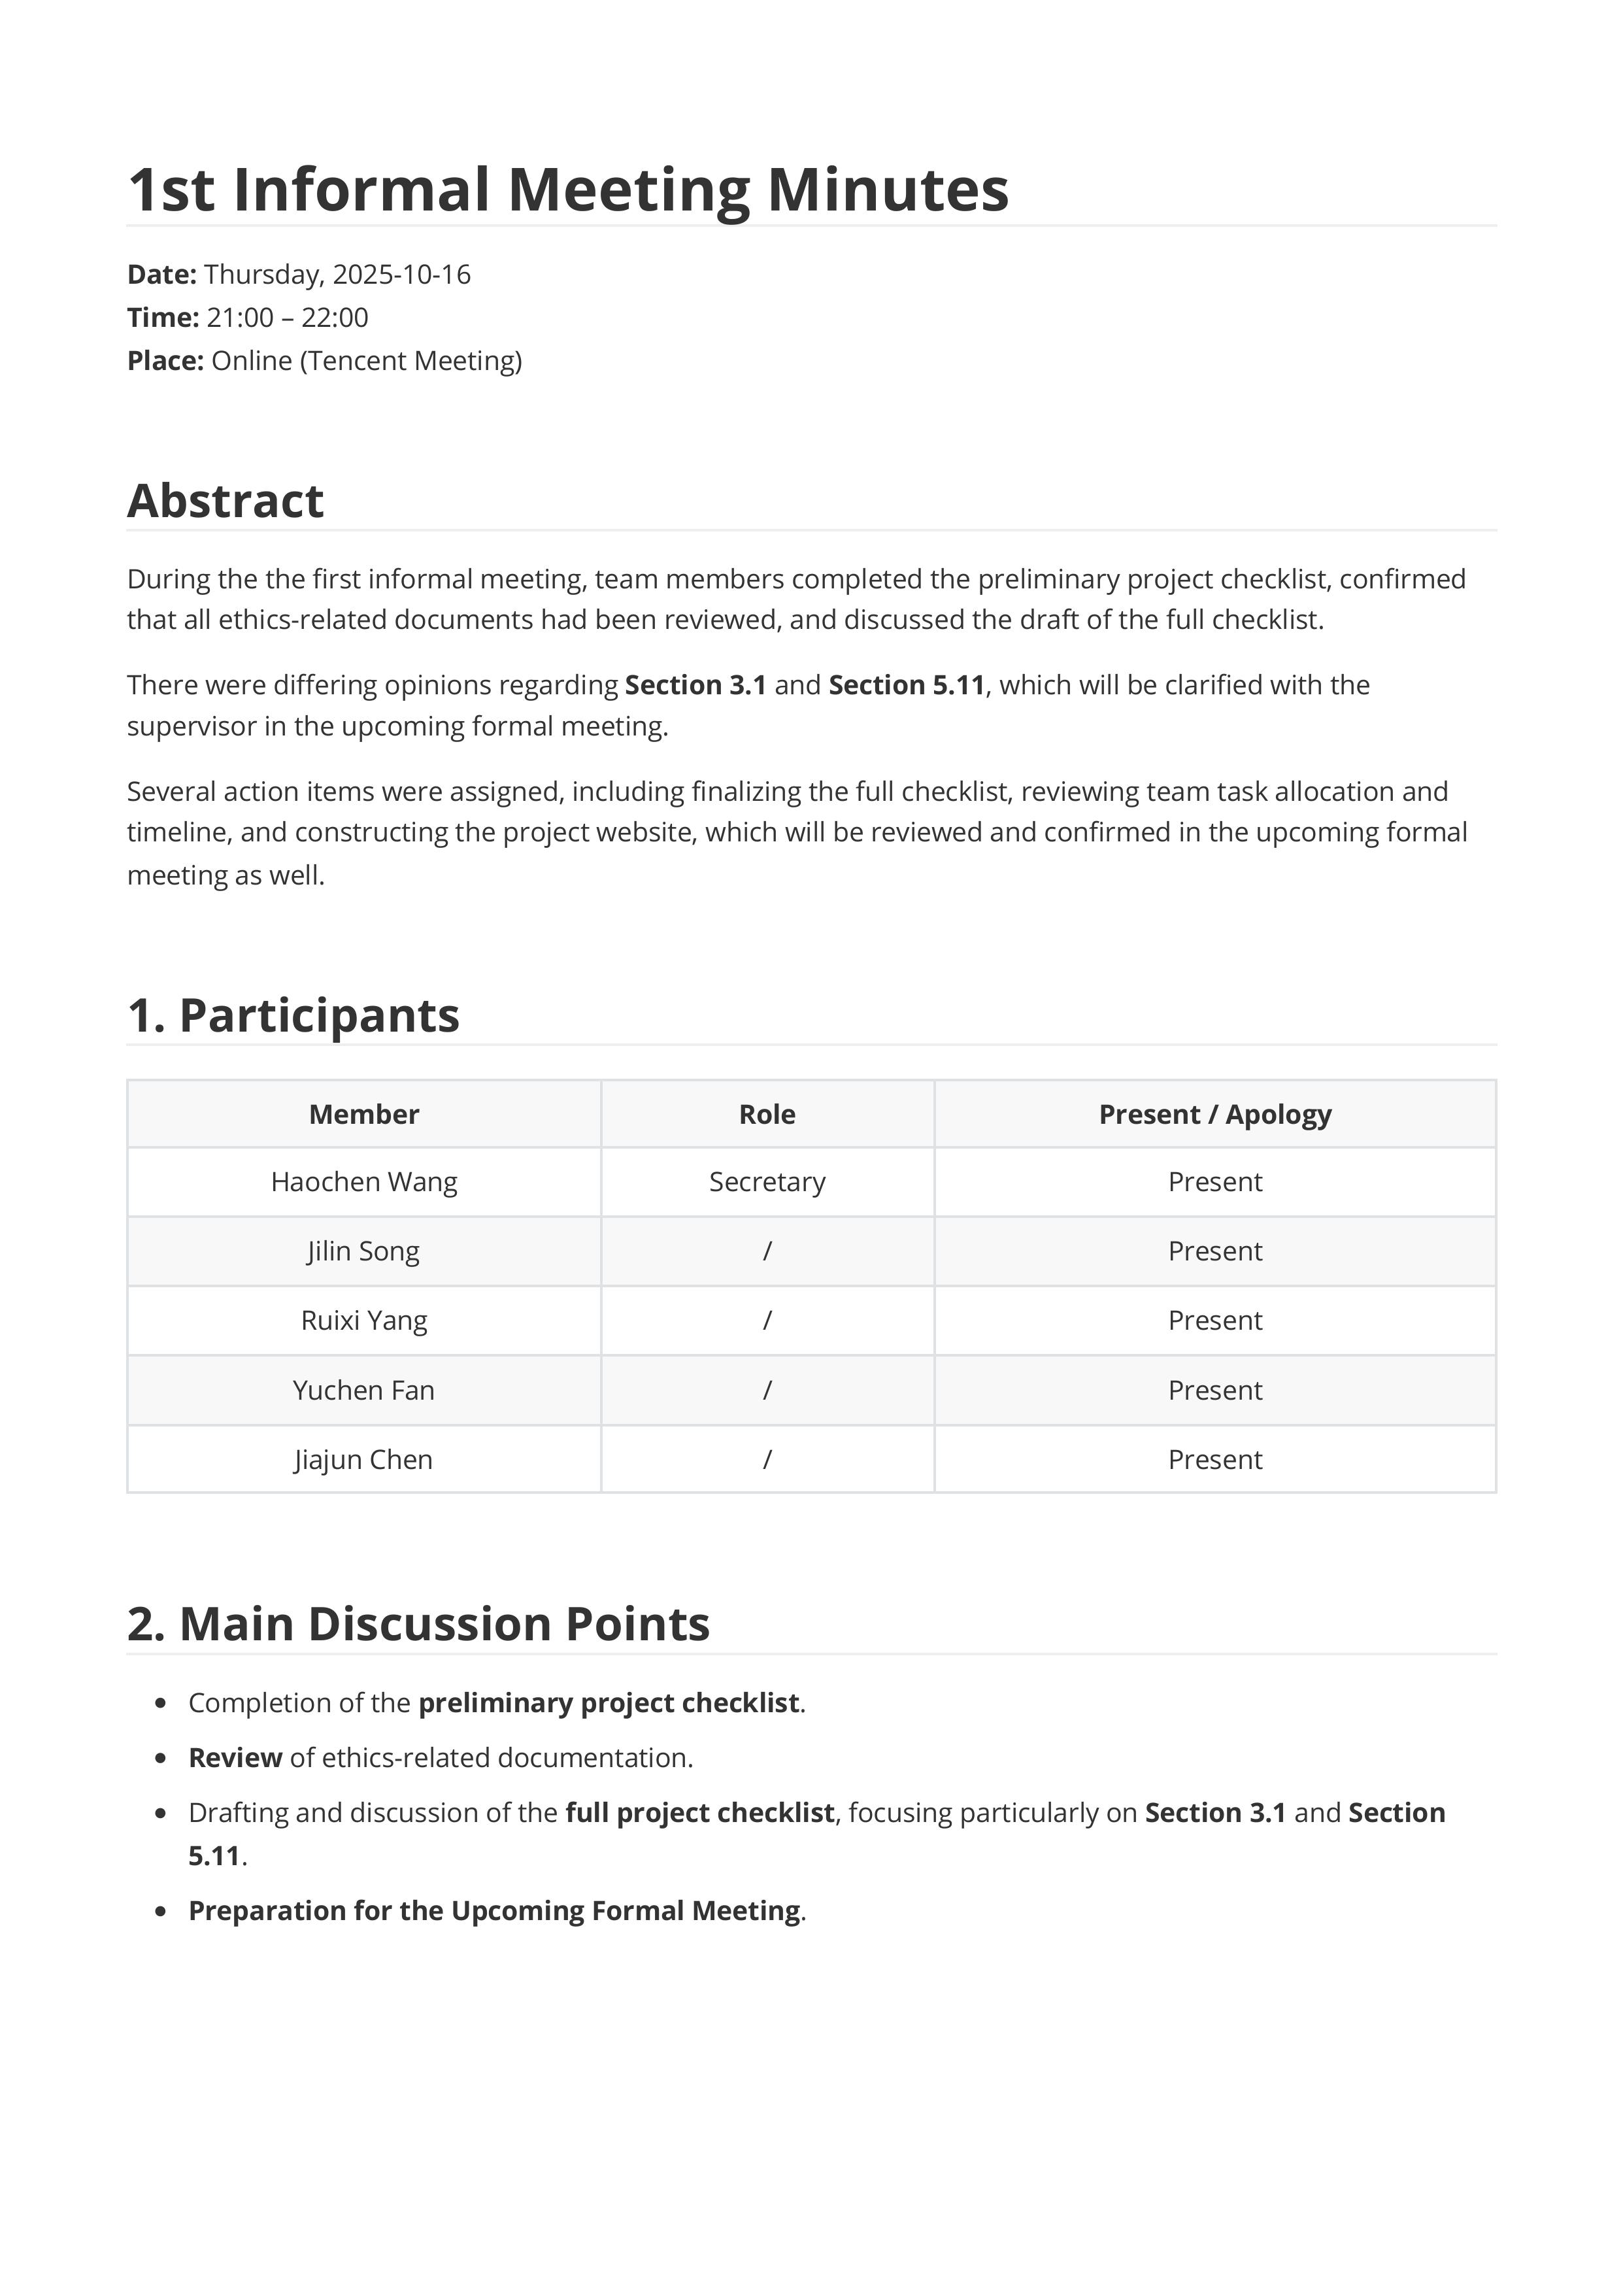
\includegraphics[width=1.0\textwidth]{images/appendix/1st_Informal_Meeting_Minutes_2025-10-16-page-0001.jpg}
\end{figure}
\begin{figure}[H]
    \centering
    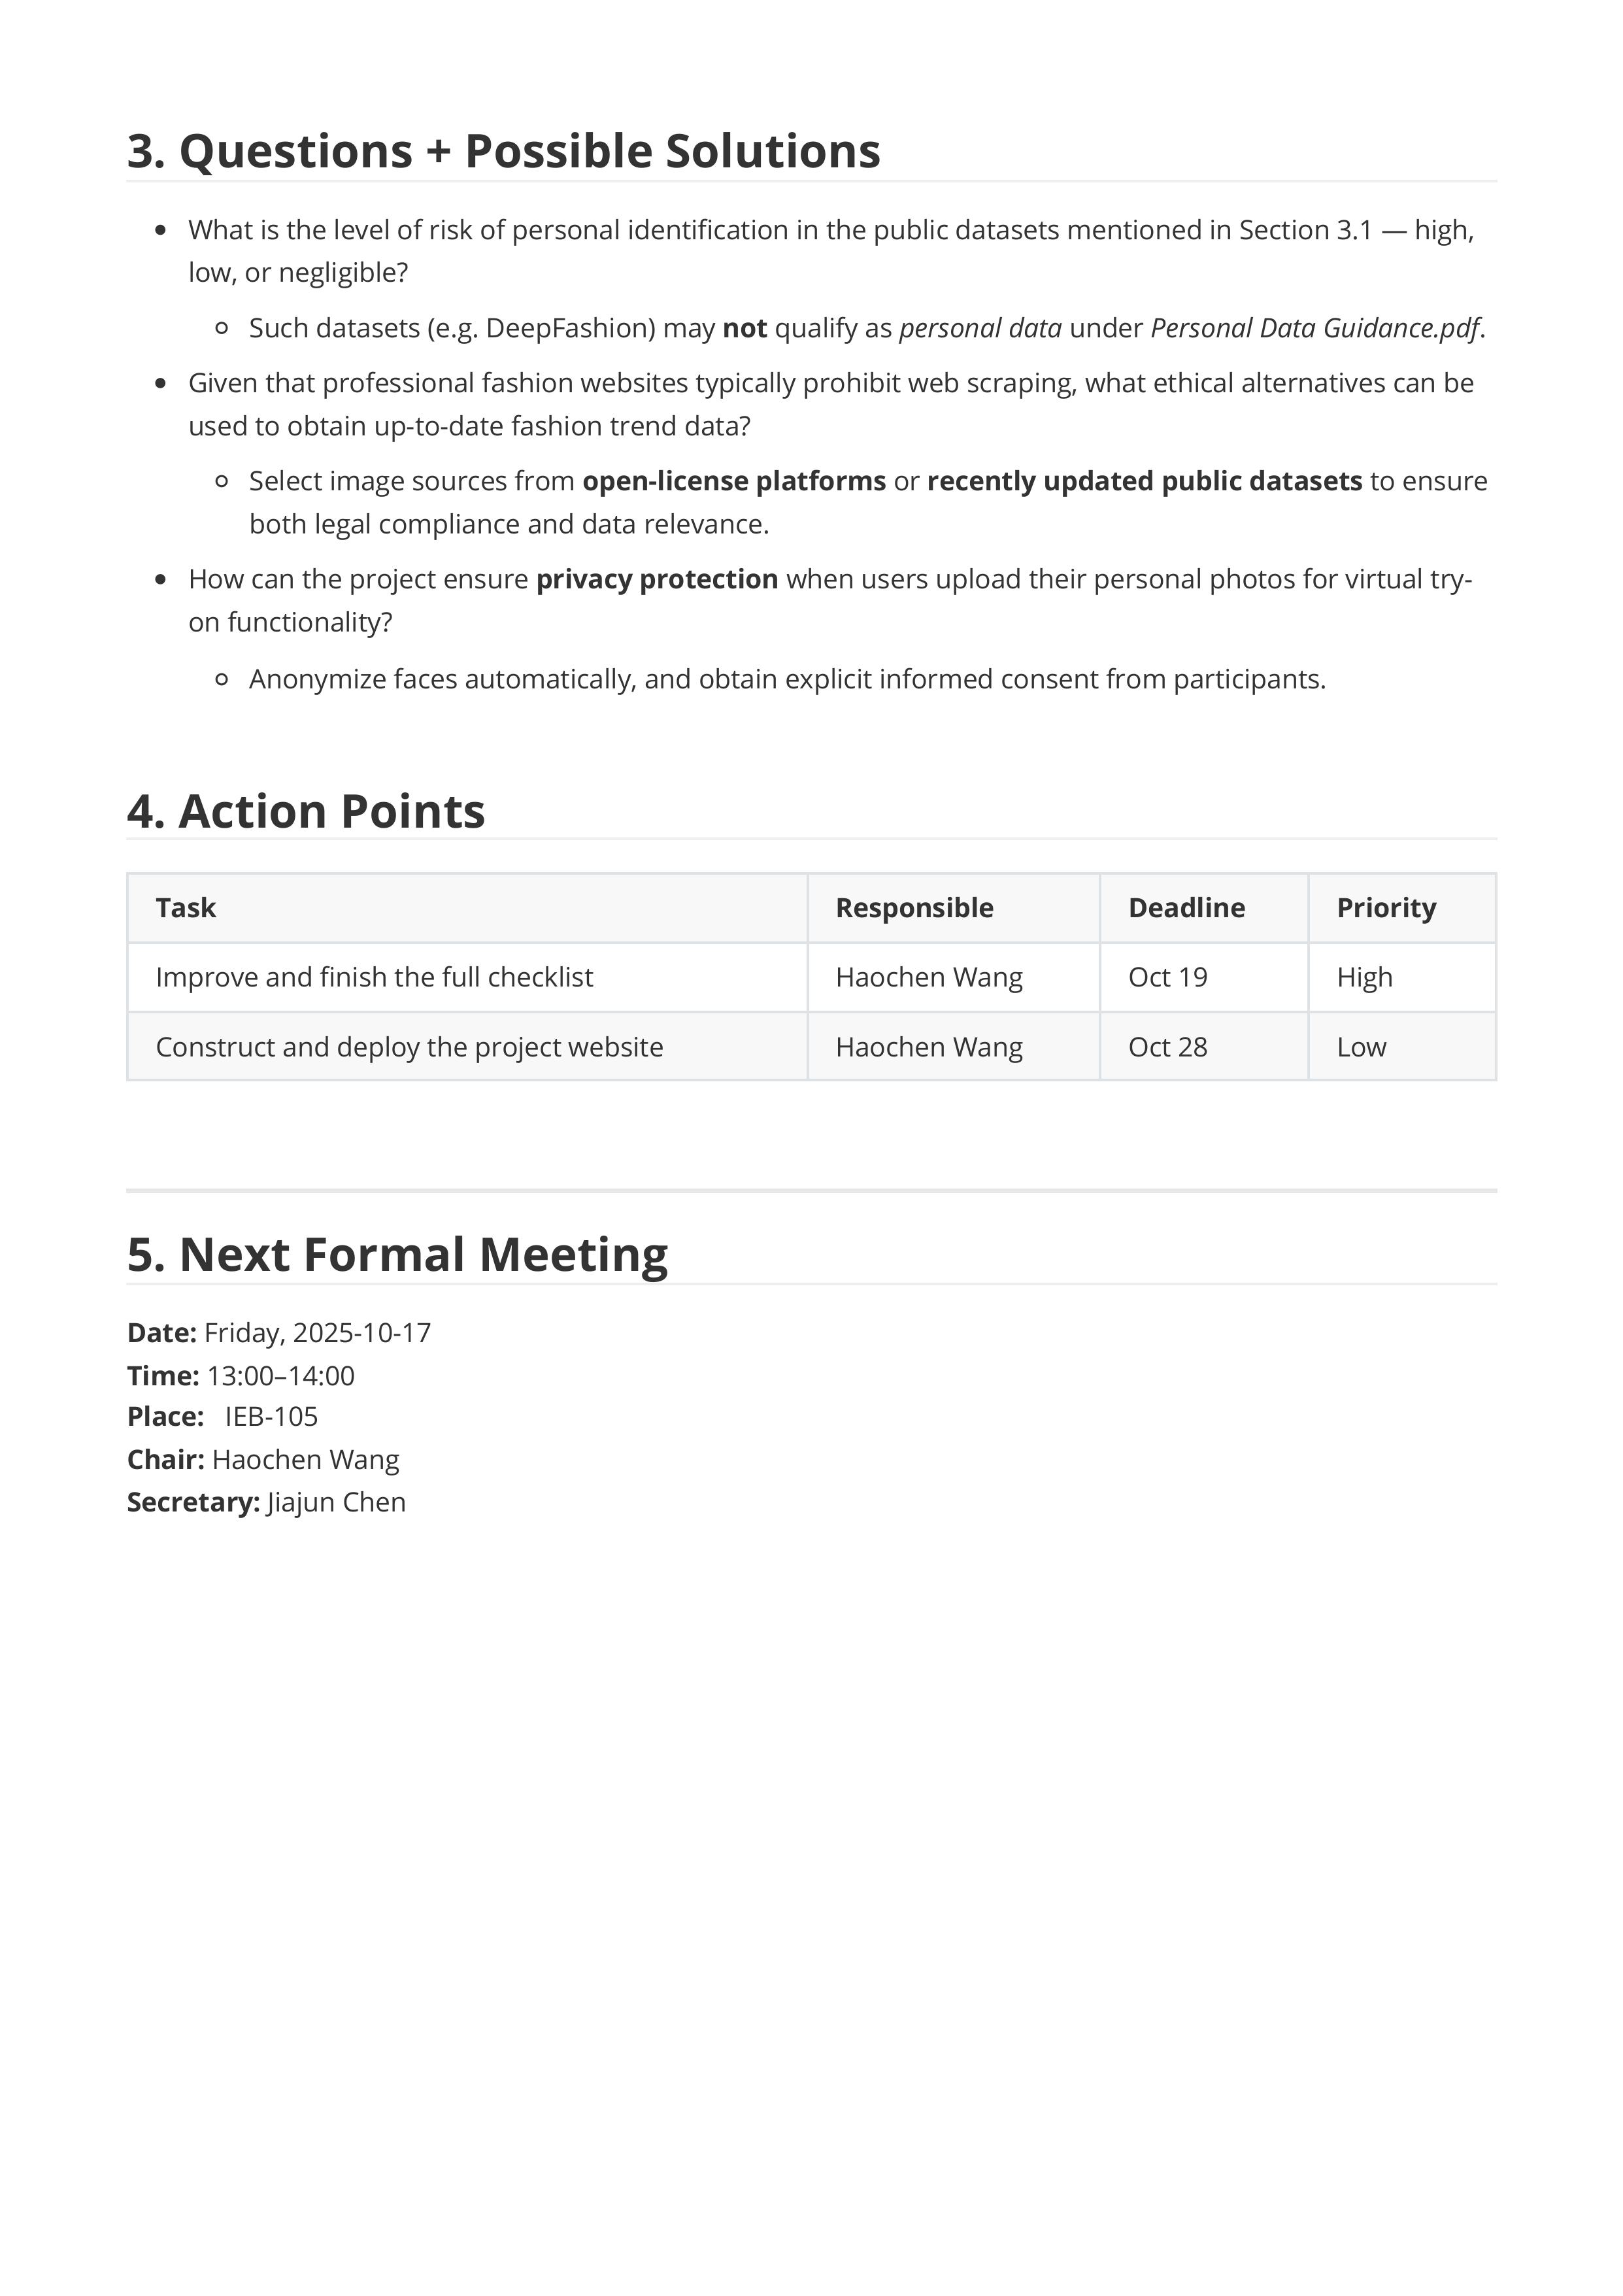
\includegraphics[width=1.0\textwidth]{images/appendix/1st_Informal_Meeting_Minutes_2025-10-16-page-0002.jpg}
\end{figure}


\section{2nd Formal Meeting Minutes (2025-10-24)}
\begin{figure}[H]
    \centering
    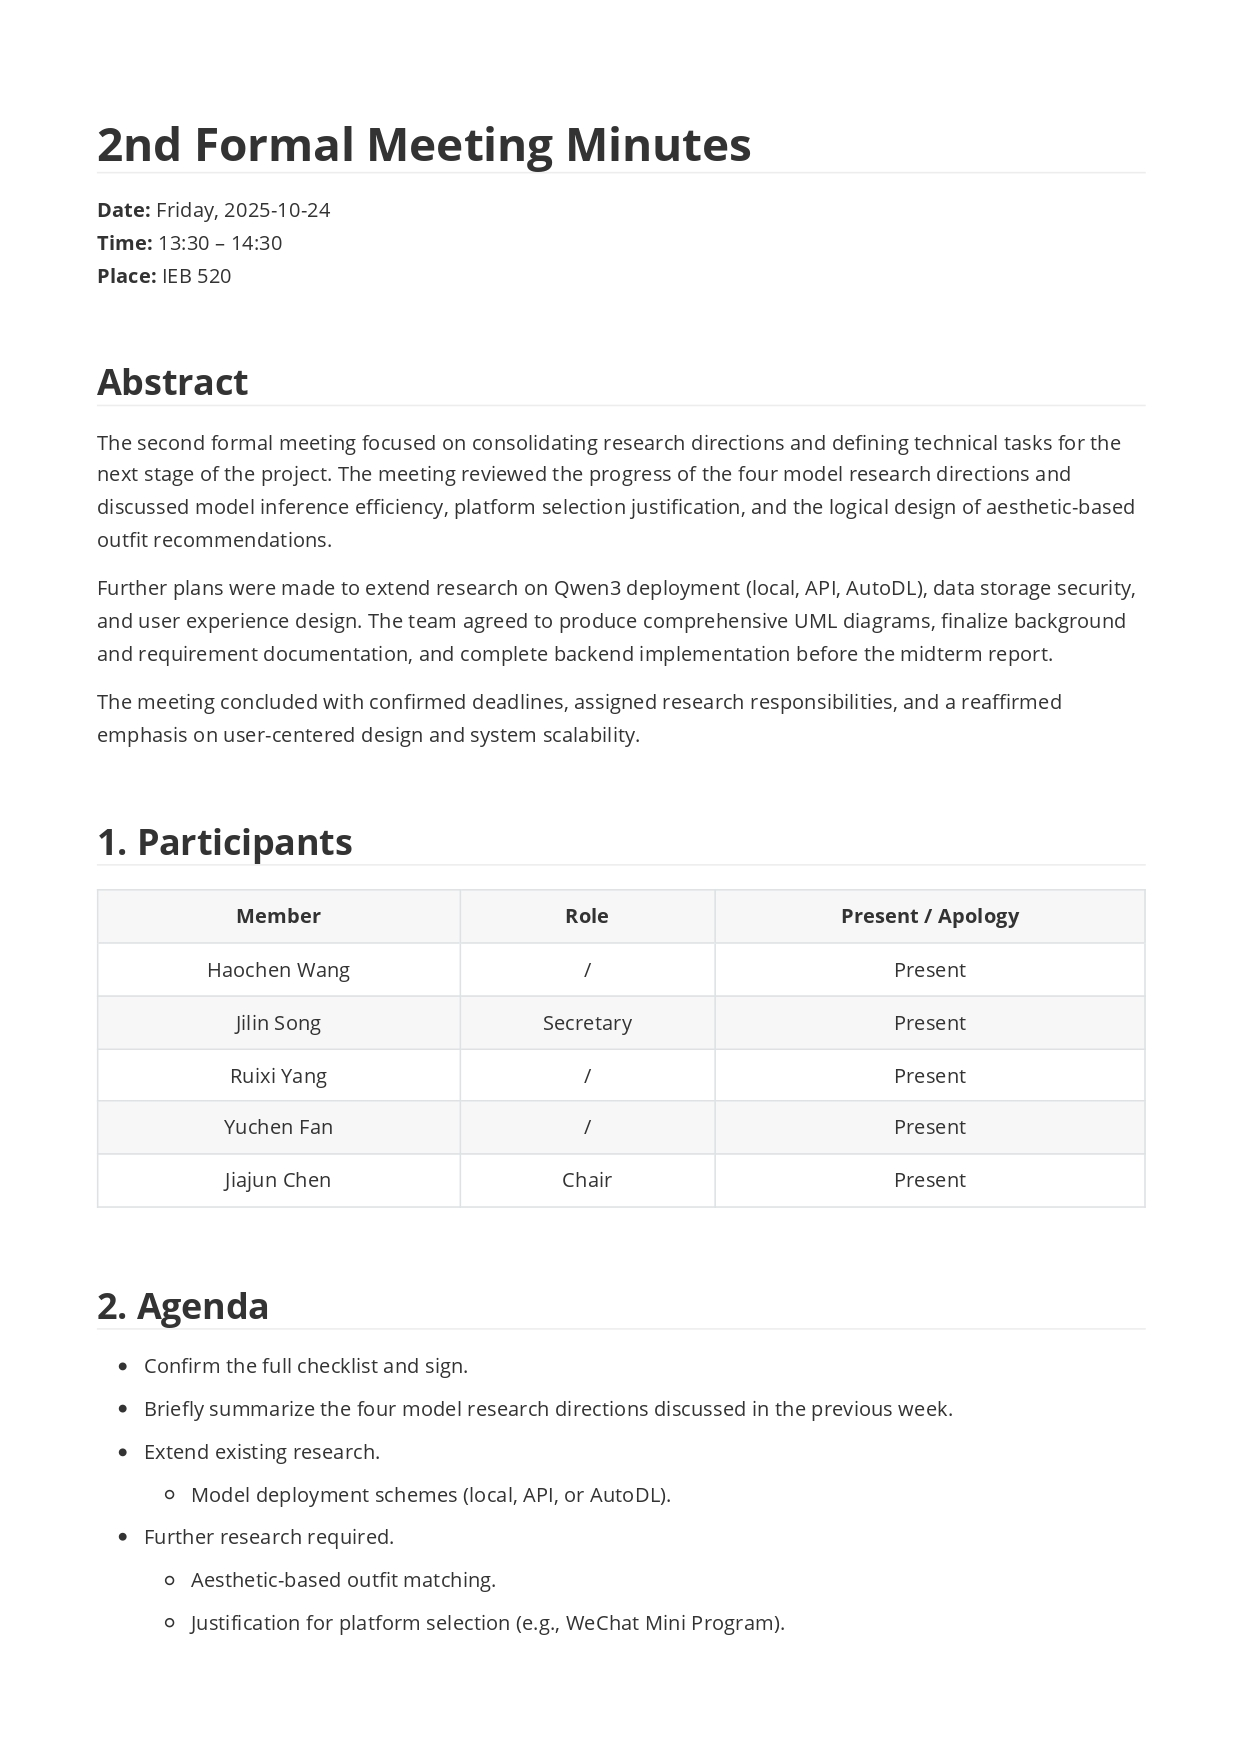
\includegraphics[width=1.0\textwidth]{images/appendix/2nd_Formal_Meeting_Minutes_2025-10-24_page-0001.jpg}
\end{figure}
\begin{figure}[H]
    \centering
    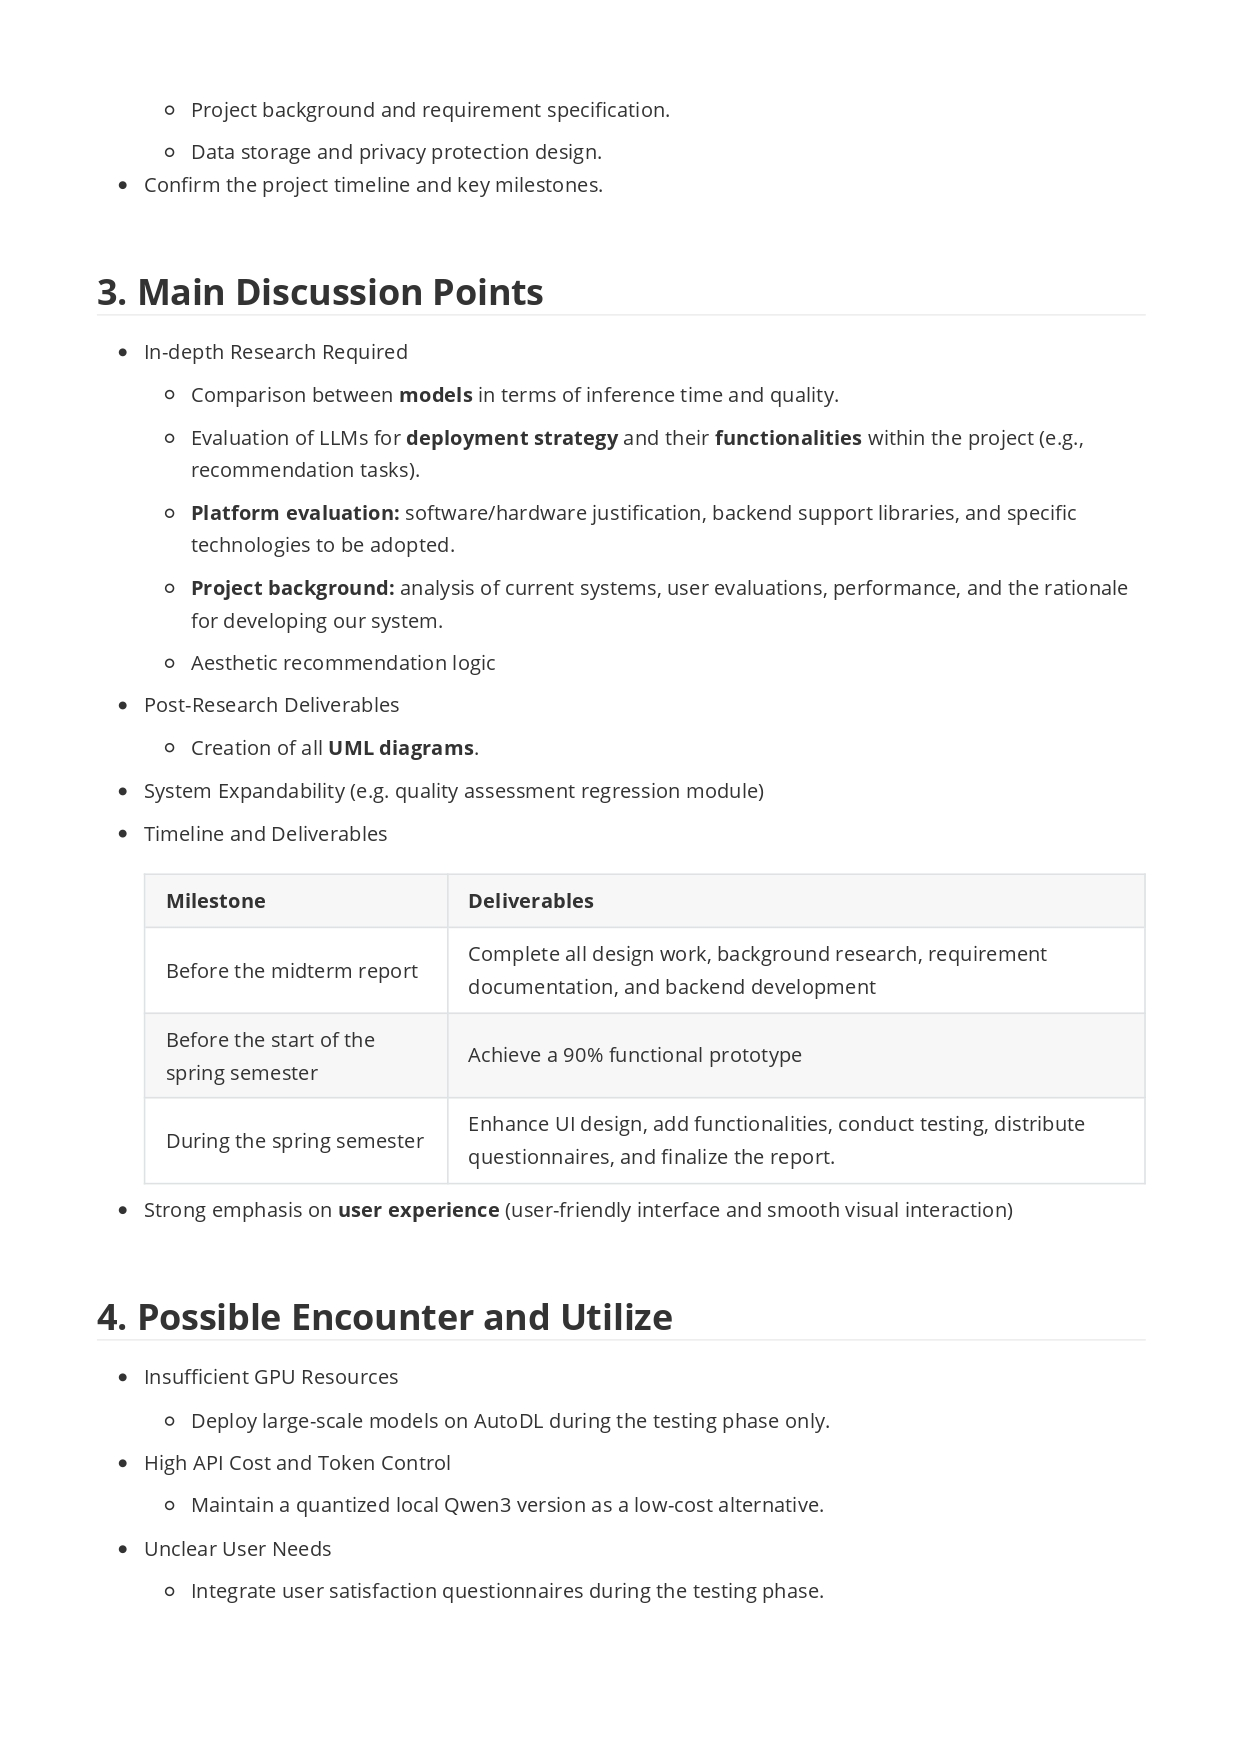
\includegraphics[width=1.0\textwidth]{images/appendix/2nd_Formal_Meeting_Minutes_2025-10-24_page-0002.jpg}
\end{figure}
\begin{figure}[H]
    \centering
    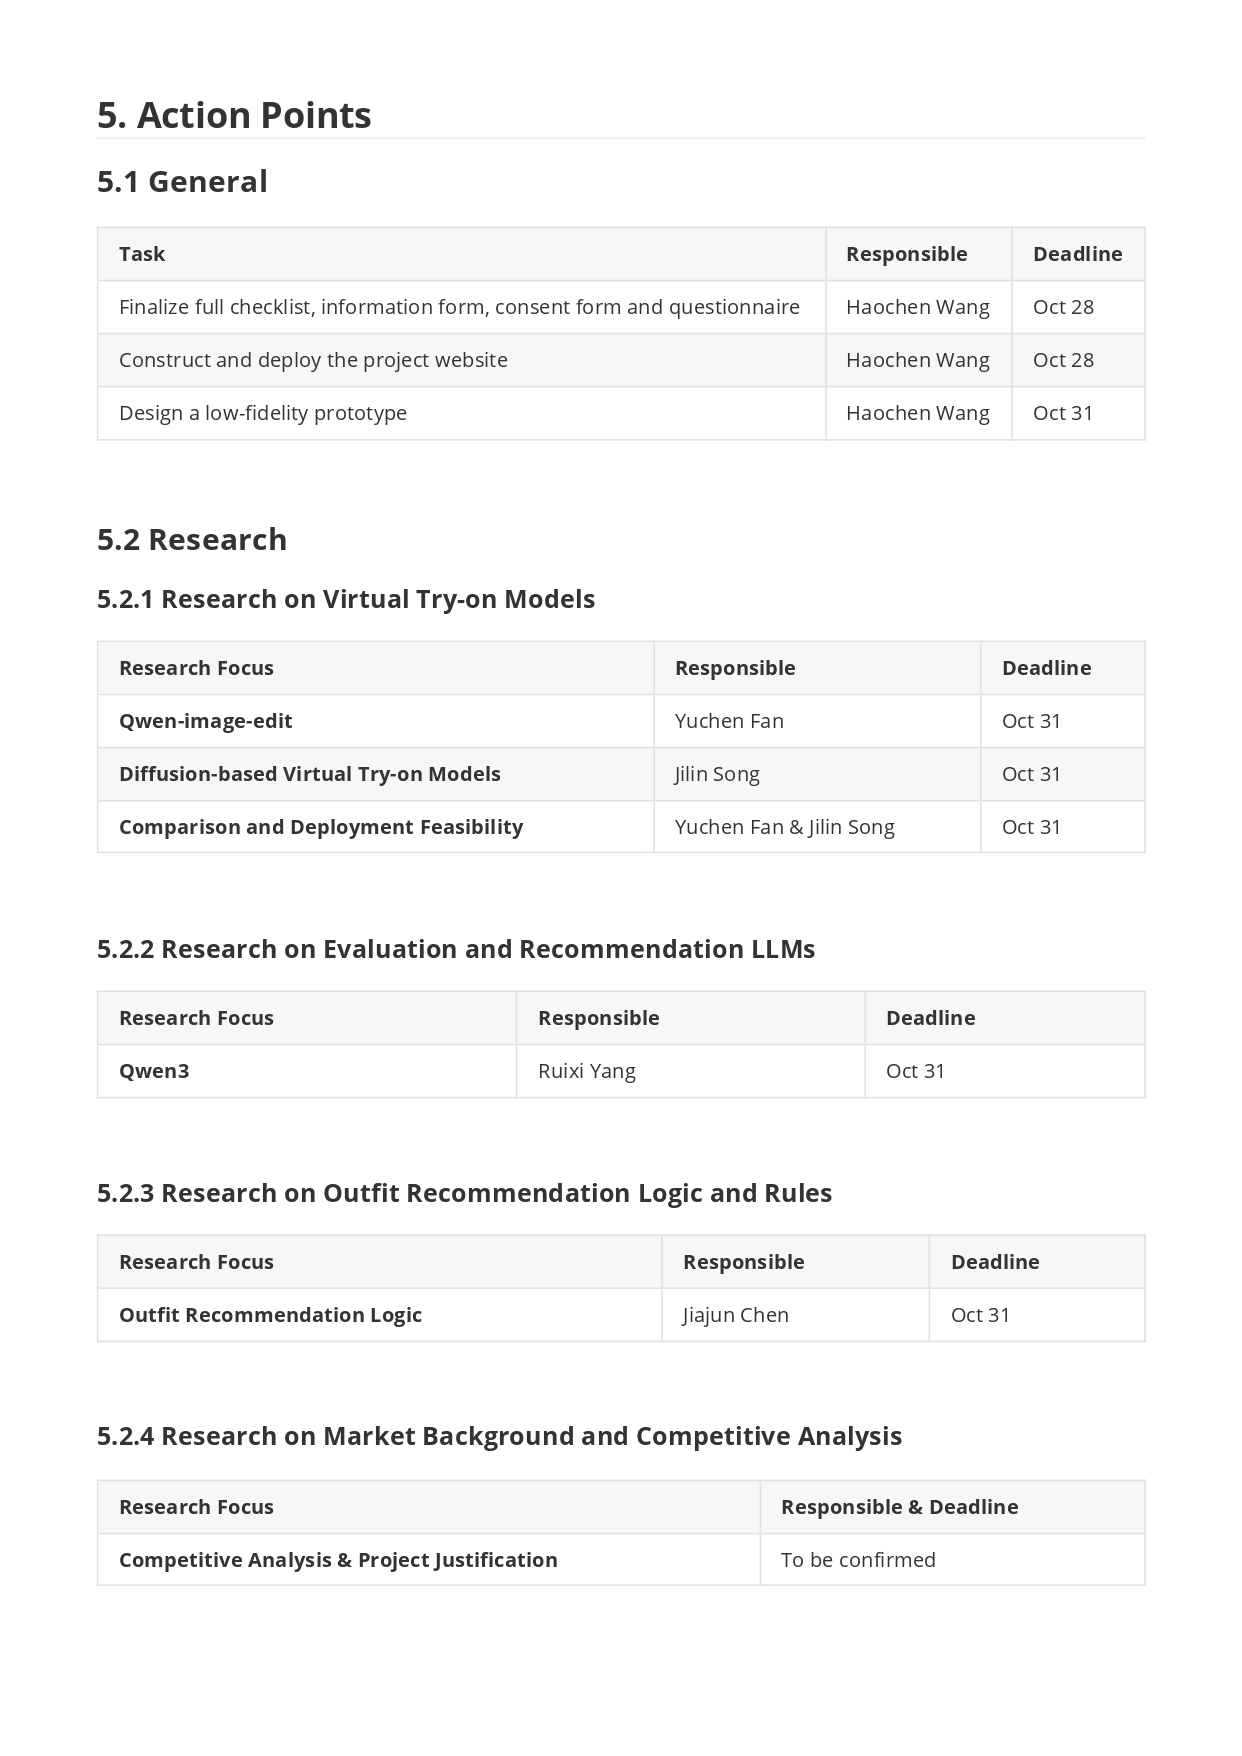
\includegraphics[width=1.0\textwidth]{images/appendix/2nd_Formal_Meeting_Minutes_2025-10-24_page-0003.jpg}
\end{figure}
\begin{figure}[H]
    \centering
    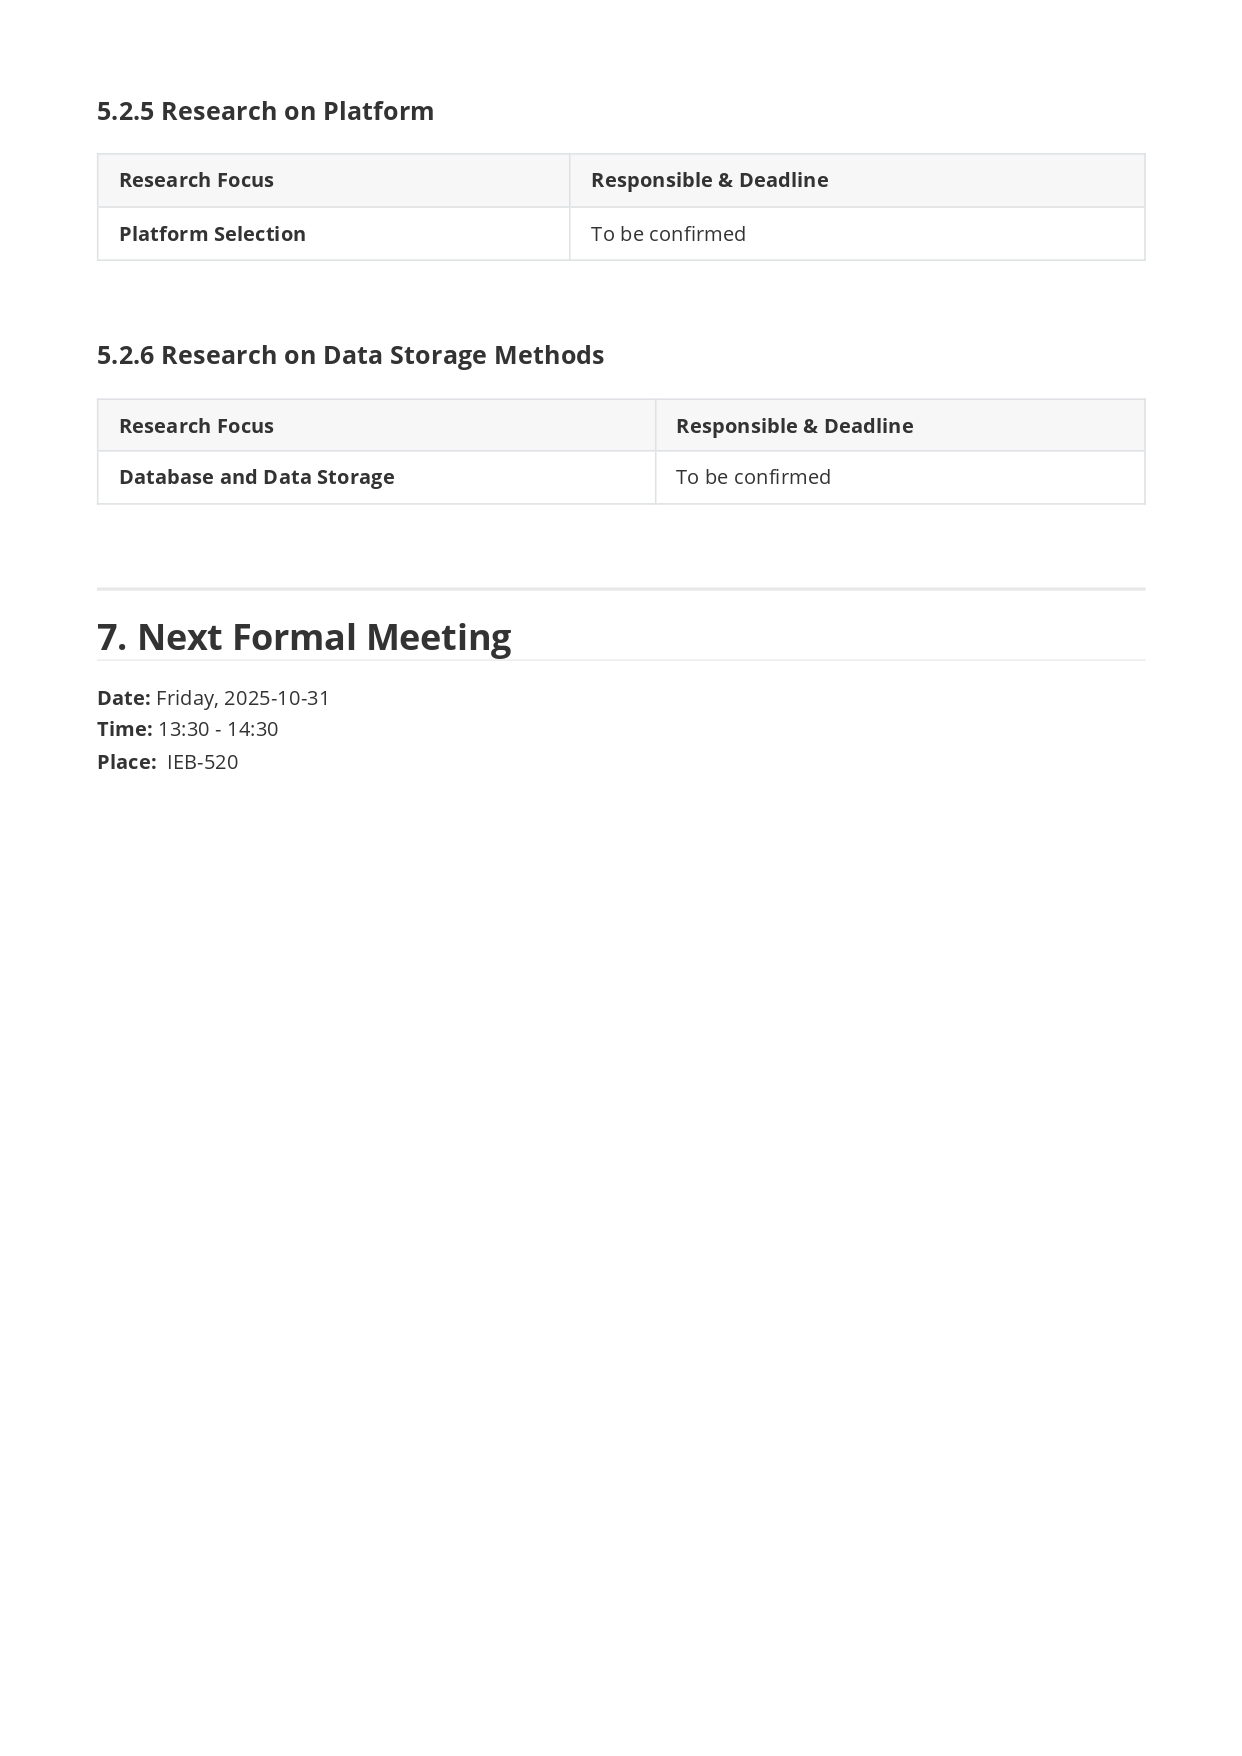
\includegraphics[width=1.0\textwidth]{images/appendix/2nd_Formal_Meeting_Minutes_2025-10-24_page-0004.jpg}
\end{figure}


\section{2nd Informal Meeting Minutes (2025-10-23)}
\begin{figure}[H]
    \centering
    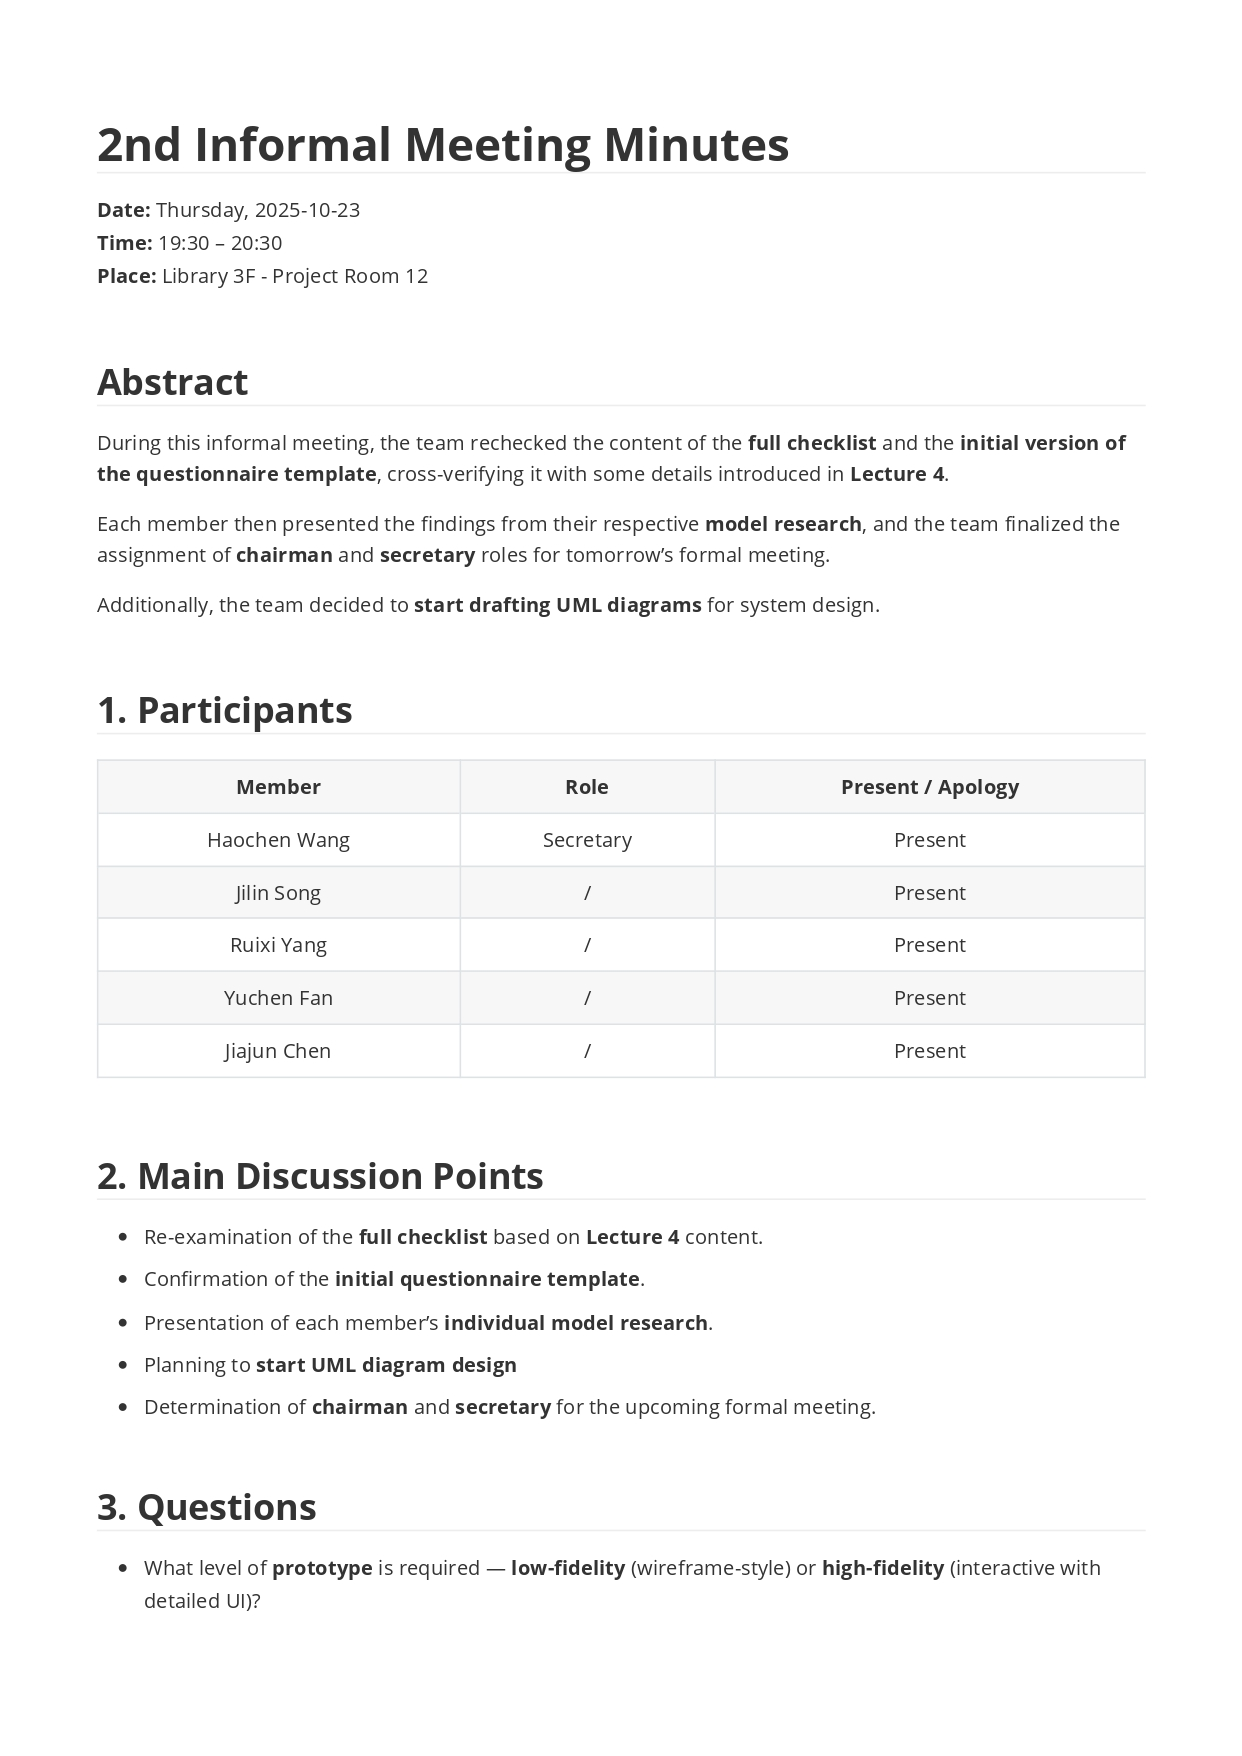
\includegraphics[width=1.0\textwidth]{images/appendix/2nd_Informal_Meeting_Minutes_2025-10-23_page-0001.jpg}
\end{figure}
\begin{figure}[H]
    \centering
    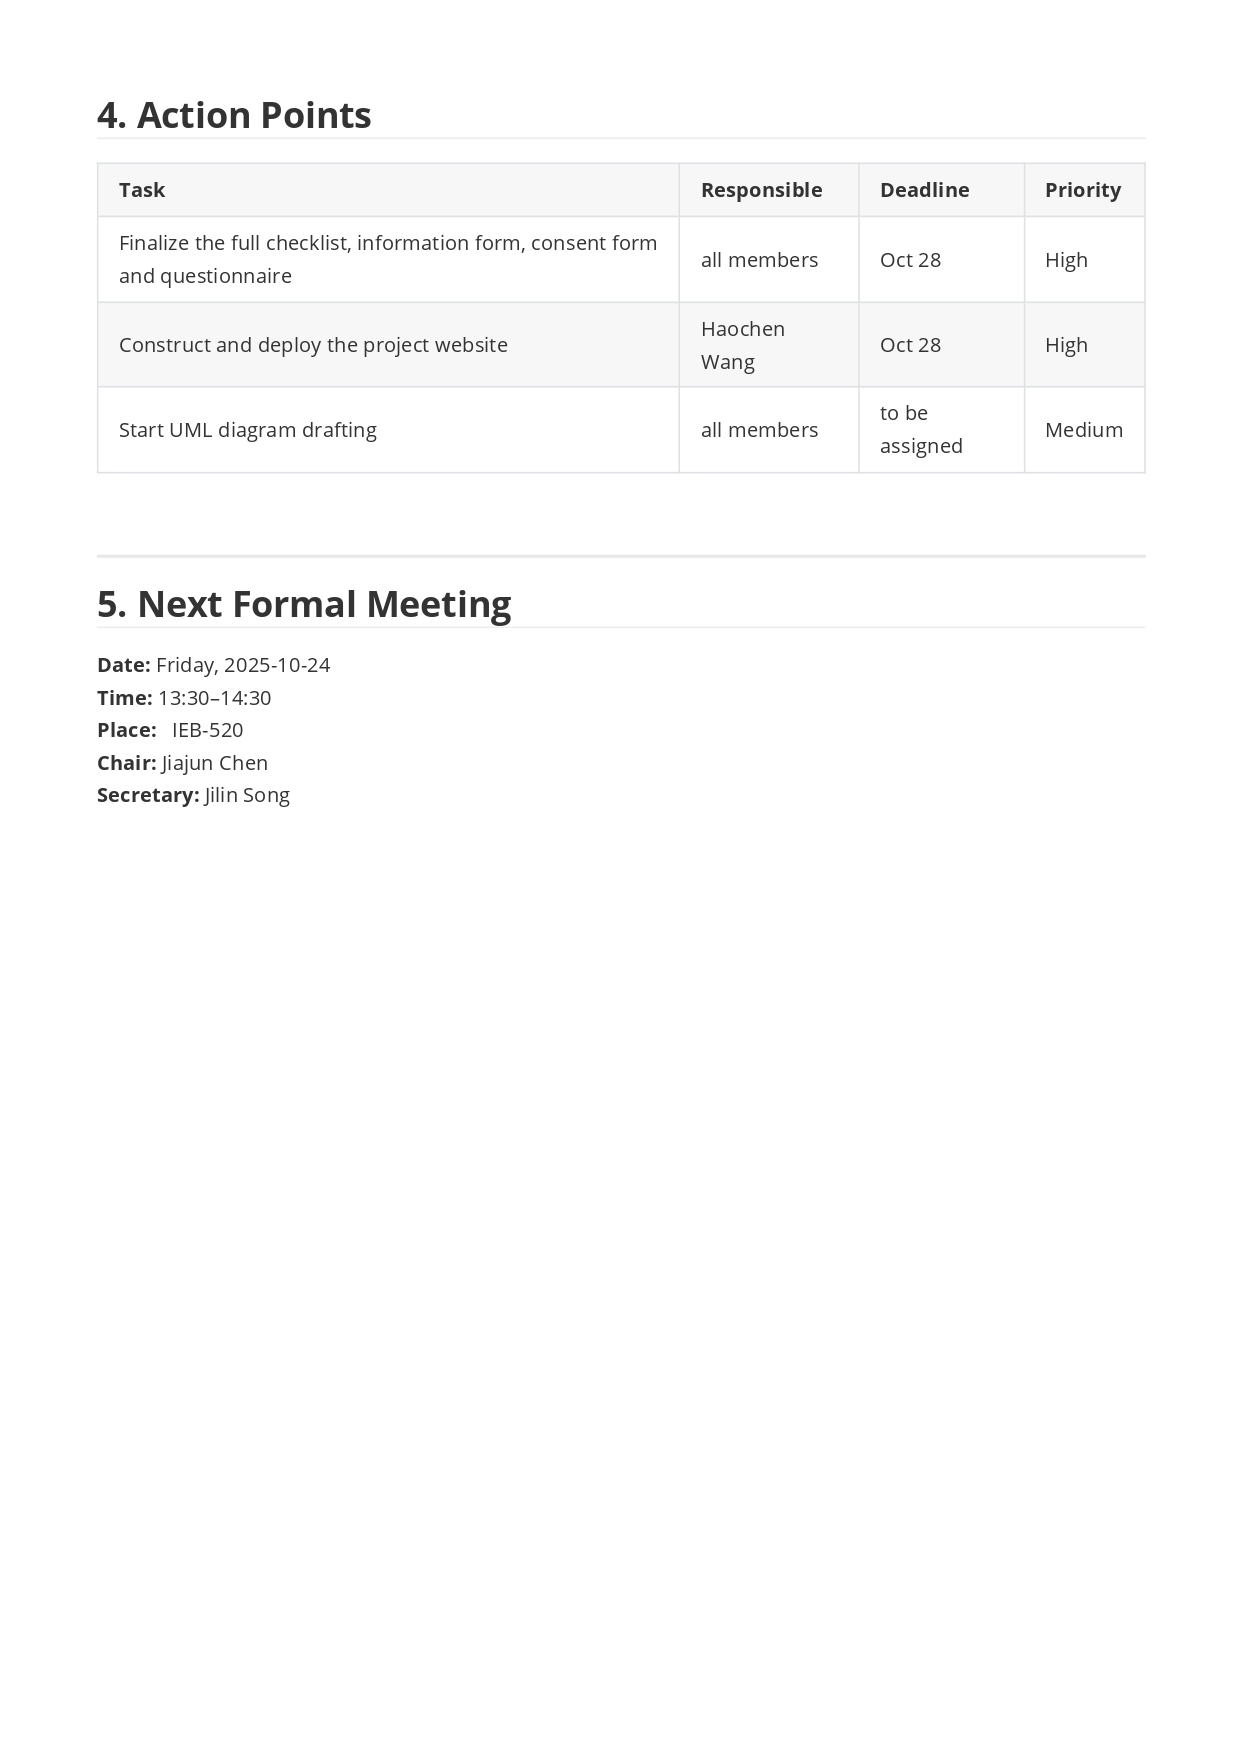
\includegraphics[width=1.0\textwidth]{images/appendix/2nd_Informal_Meeting_Minutes_2025-10-23_page-0002.jpg}
\end{figure}


\section{3rd Formal Meeting Minutes (2025-10-31)}
\begin{figure}[H]
    \centering
    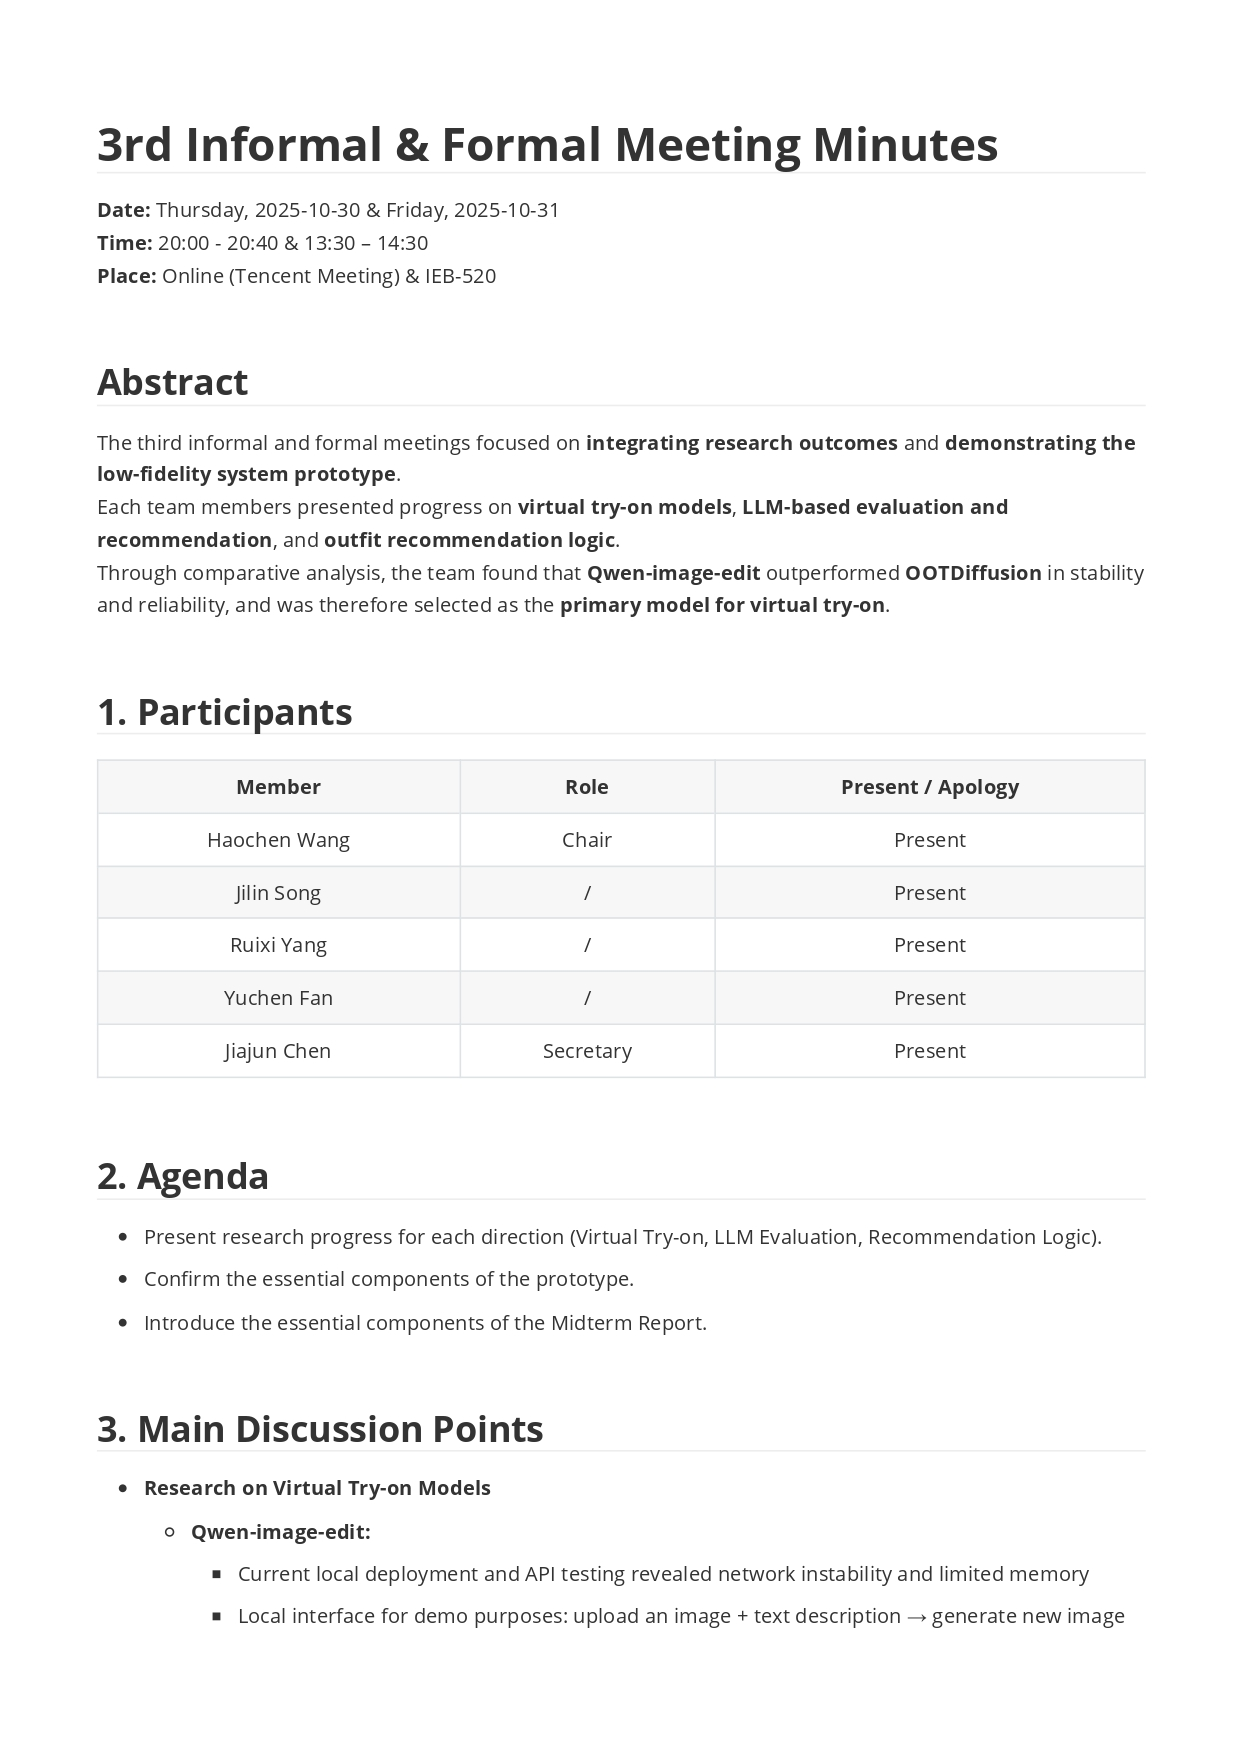
\includegraphics[width=1.0\textwidth]{images/appendix/3rd_Informal&Formal_Meeting_Minutes_2025-10-31_page-0001.jpg}
\end{figure}
\begin{figure}[H]
    \centering
    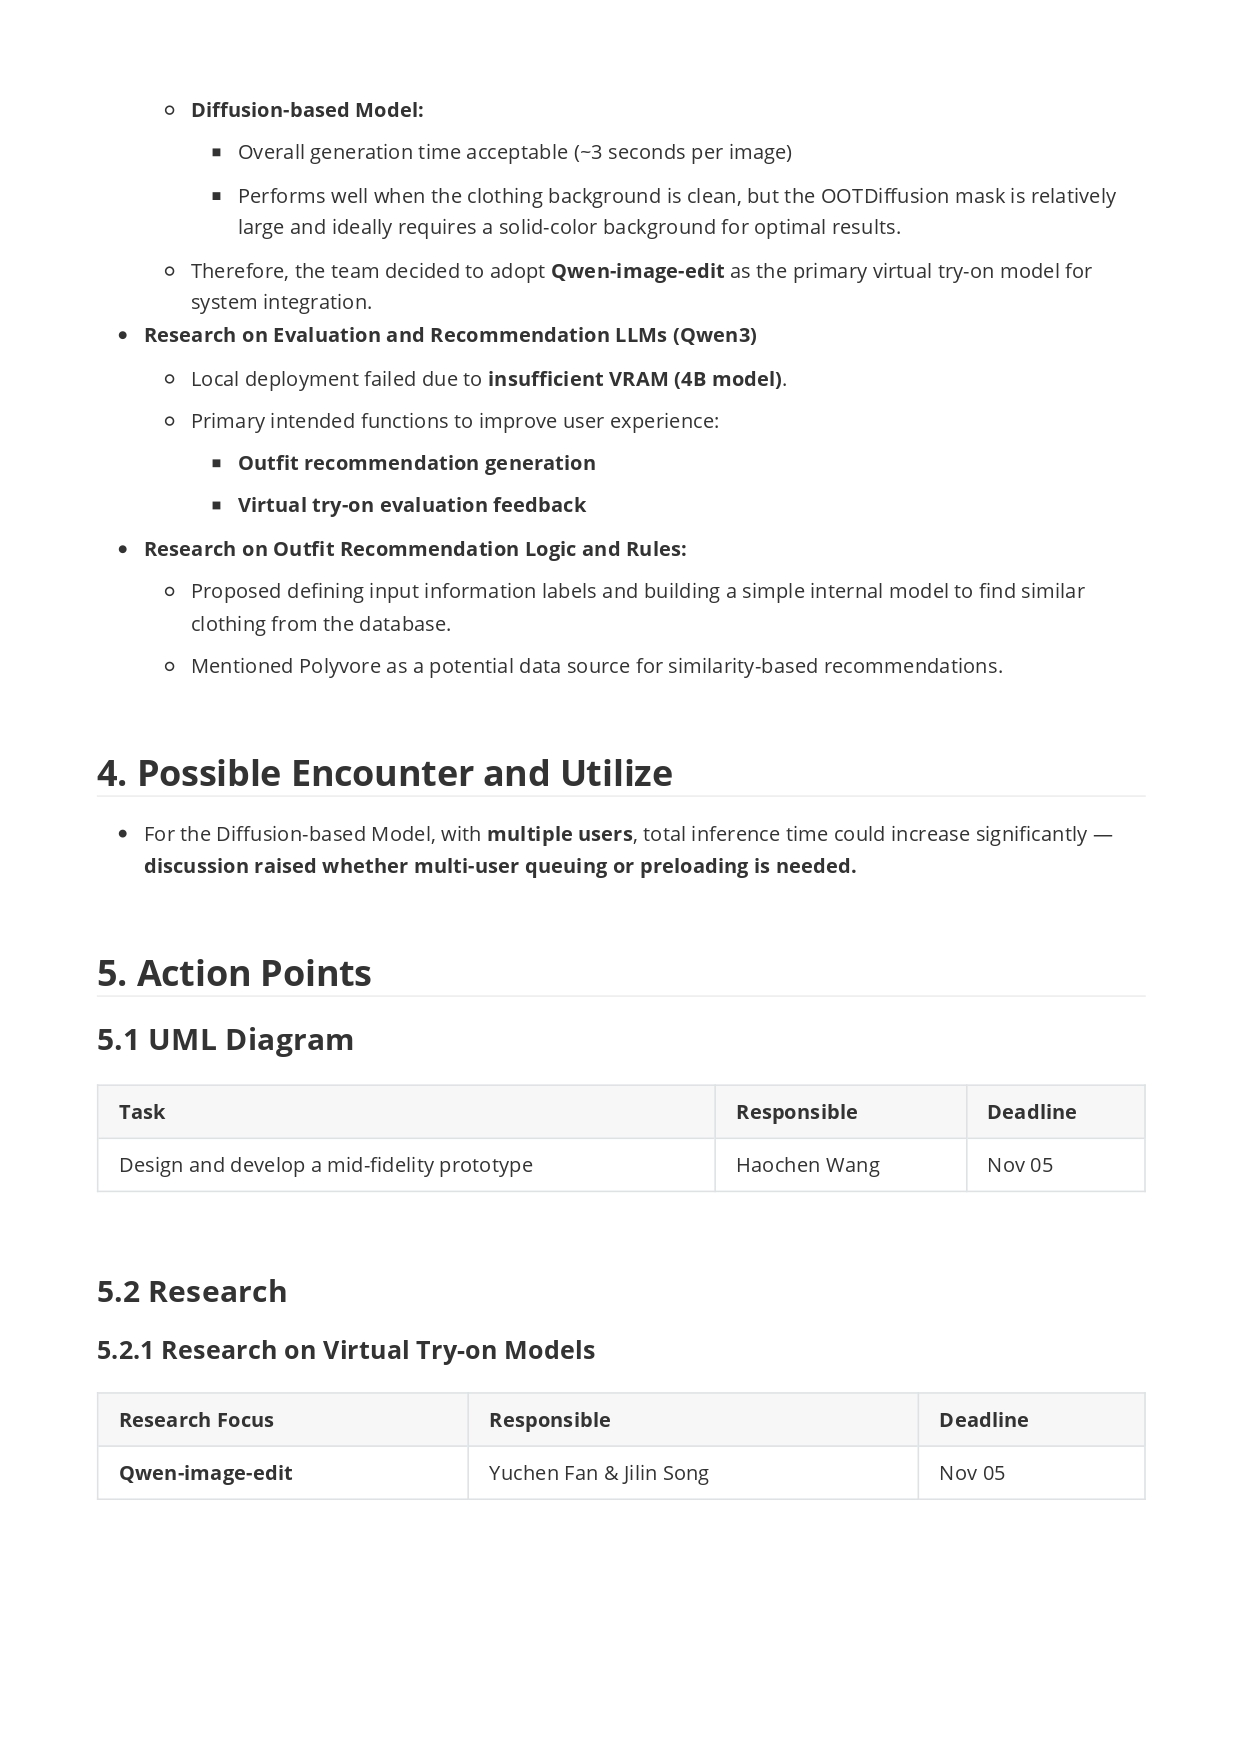
\includegraphics[width=1.0\textwidth]{images/appendix/3rd_Informal&Formal_Meeting_Minutes_2025-10-31_page-0002.jpg}
\end{figure}
\begin{figure}[H]
    \centering
    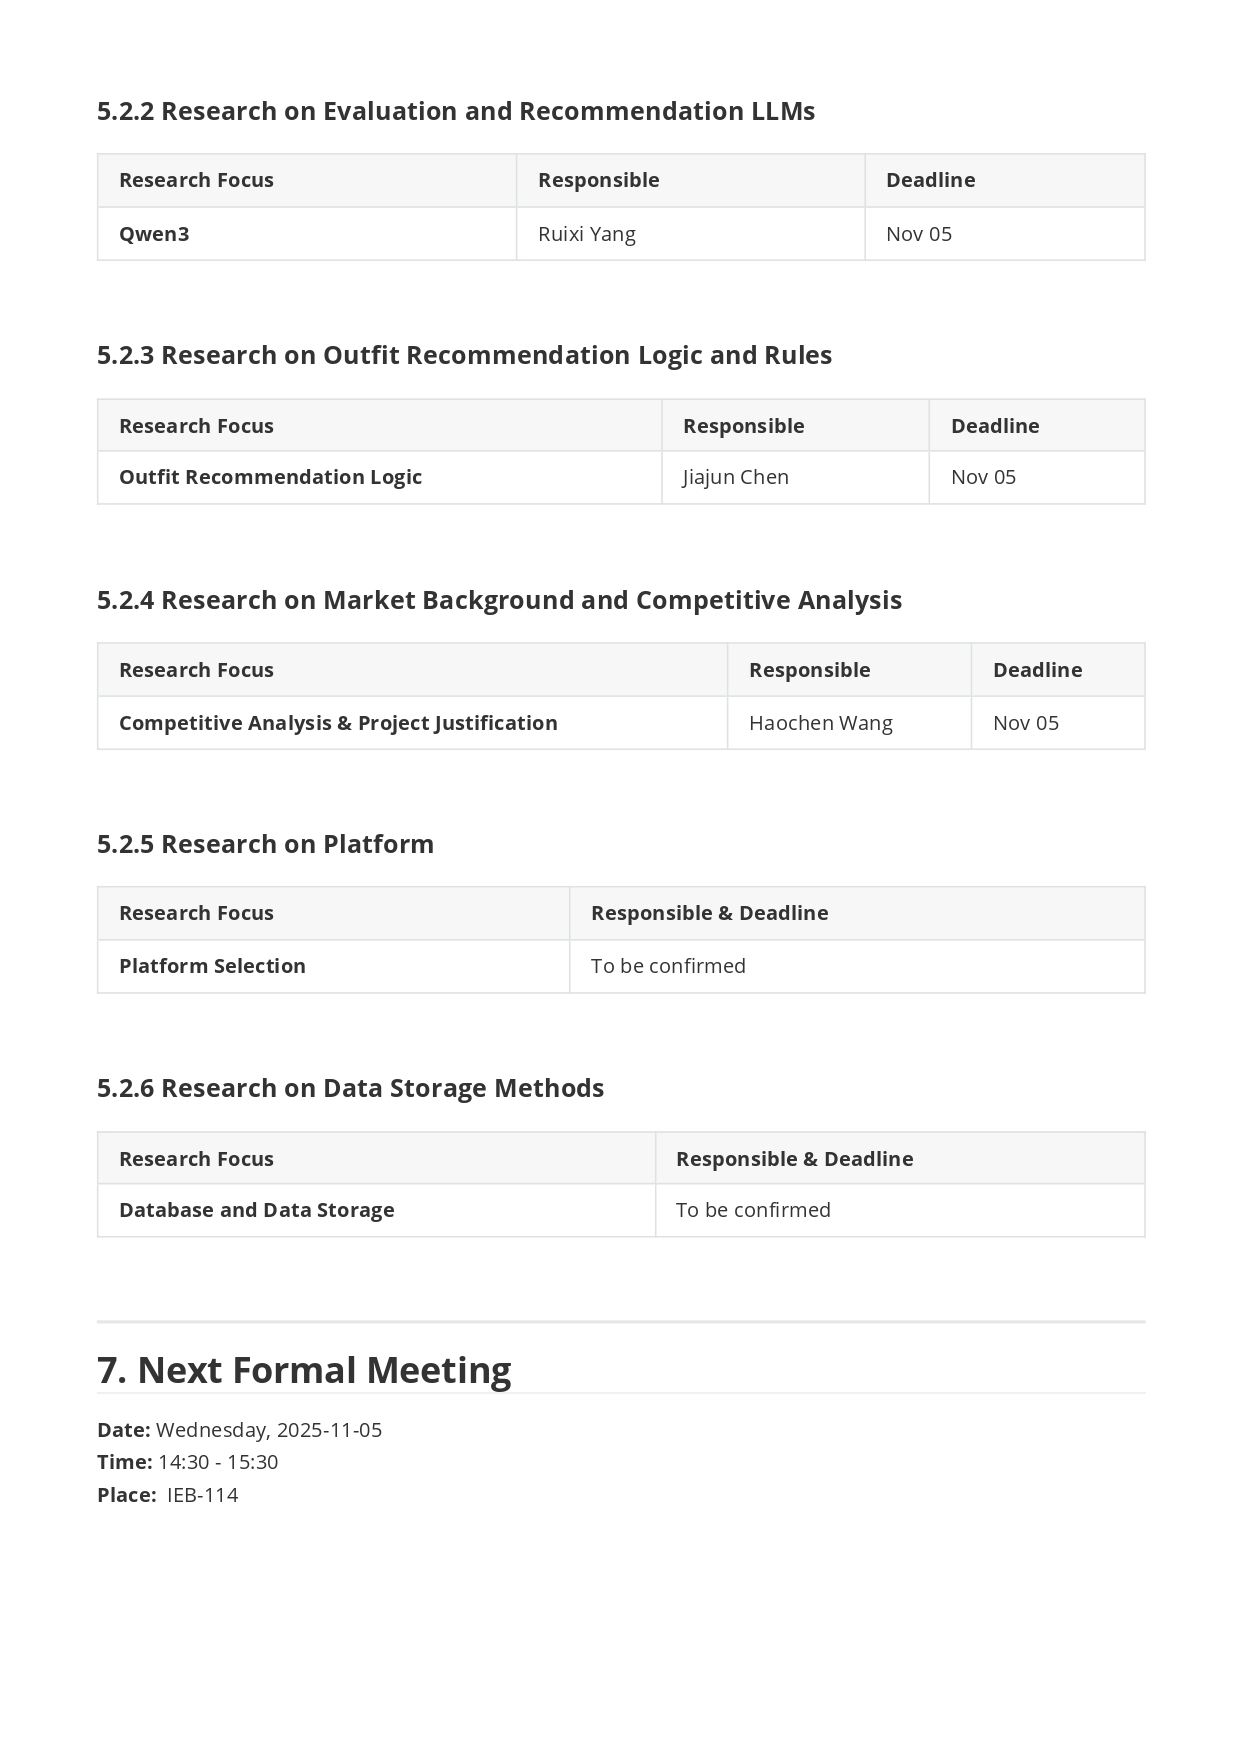
\includegraphics[width=1.0\textwidth]{images/appendix/3rd_Informal&Formal_Meeting_Minutes_2025-10-31_page-0003.jpg}
\end{figure}


\section{4th Formal Meeting Minutes (2025-11-05)}
\begin{figure}[H]
    \centering
    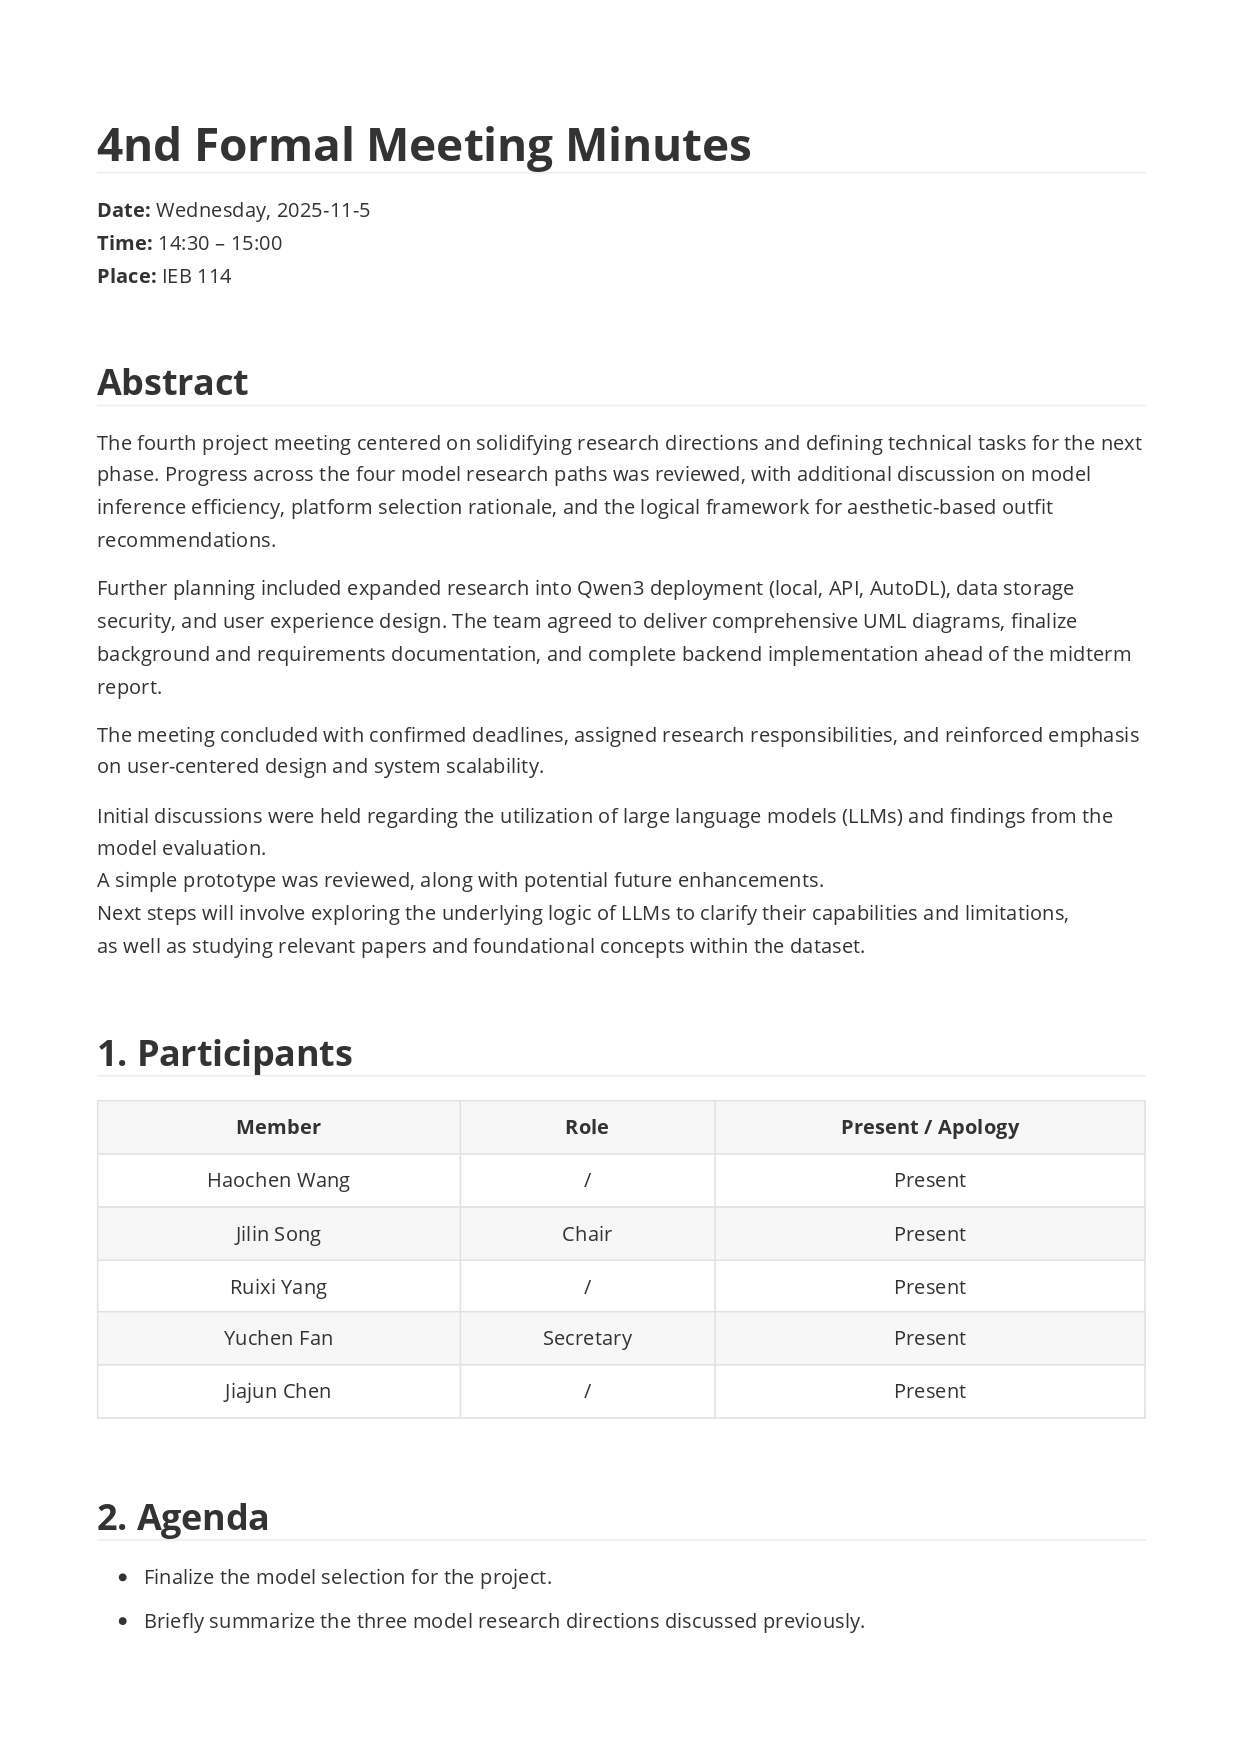
\includegraphics[width=1.0\textwidth]{images/appendix/4th_Formal_Meeting_Minutes_2025-11-05_page-0001.jpg}
\end{figure}
\begin{figure}[H]
    \centering
    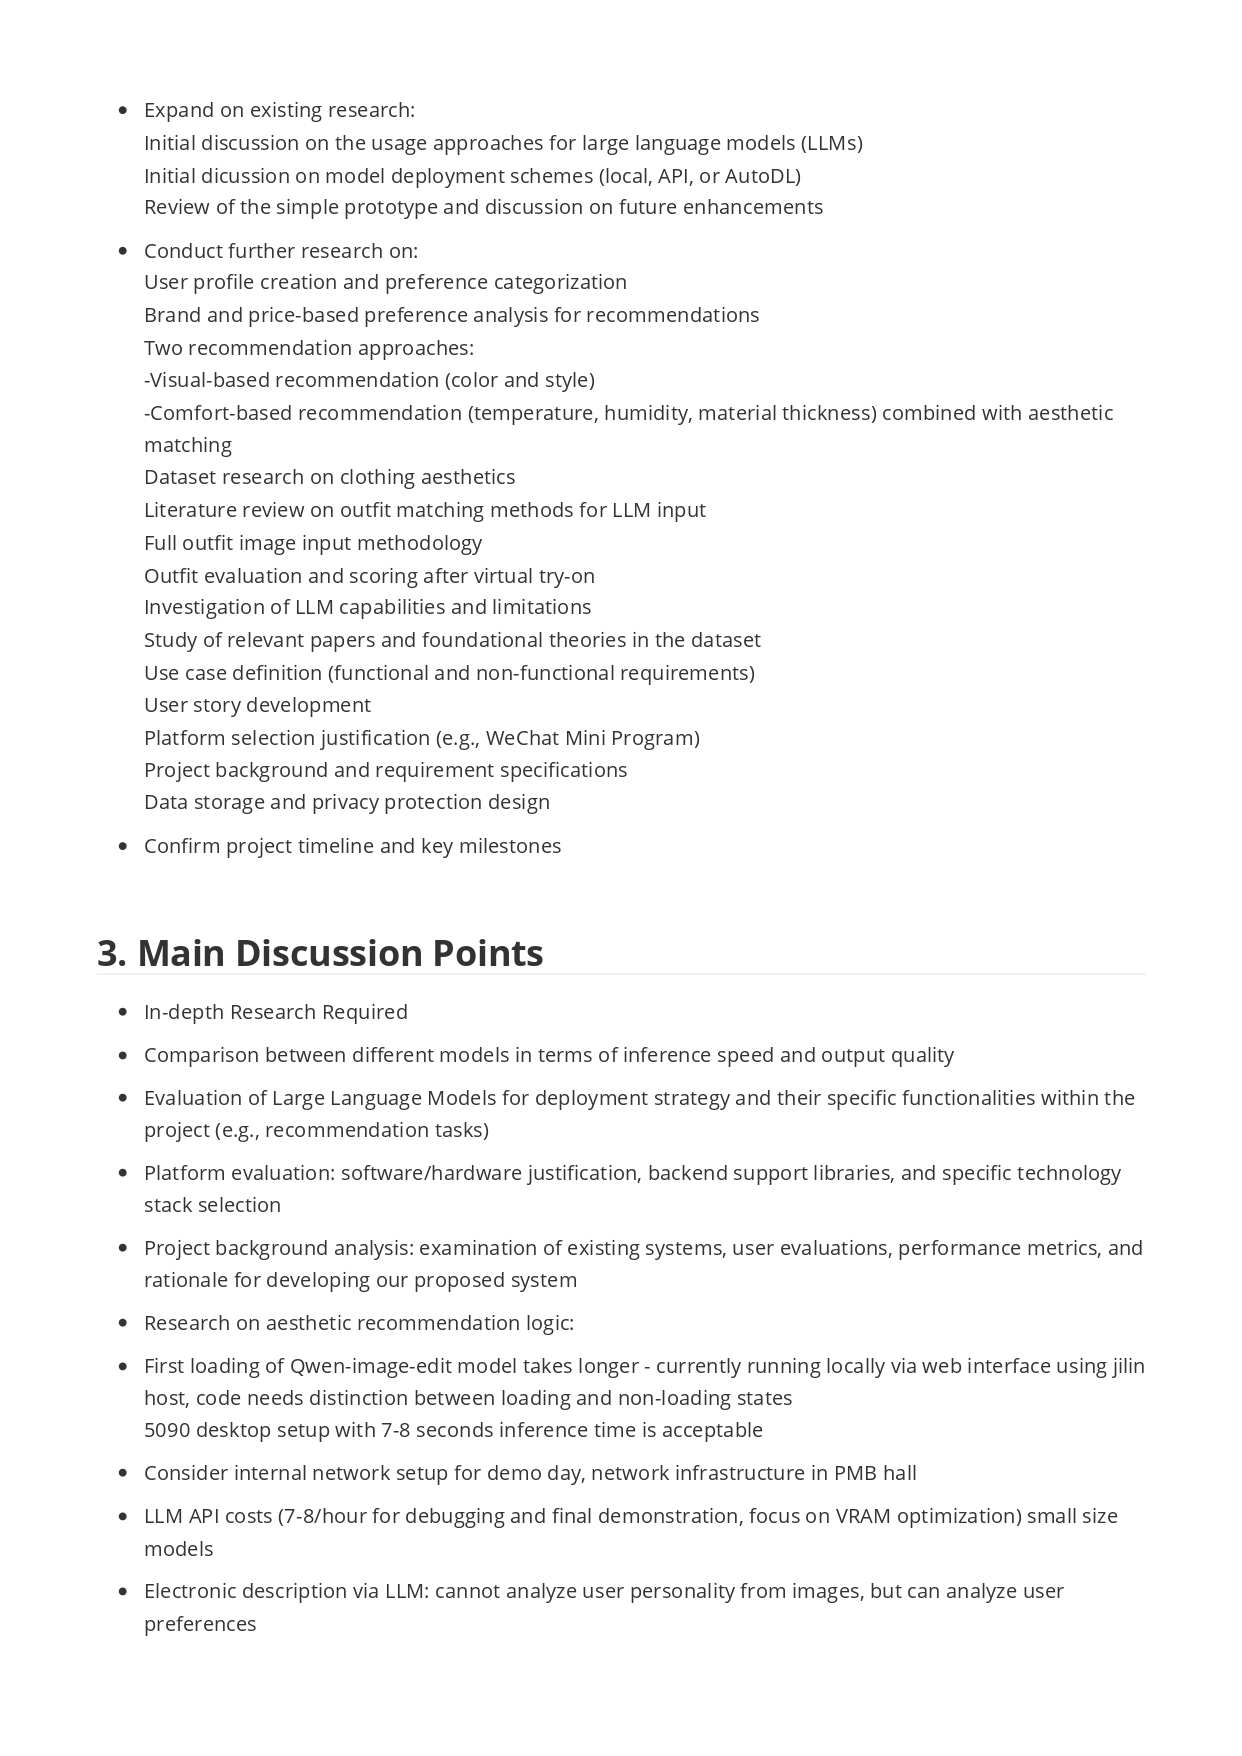
\includegraphics[width=1.0\textwidth]{images/appendix/4th_Formal_Meeting_Minutes_2025-11-05_page-0002.jpg}
\end{figure}
\begin{figure}[H]
    \centering
    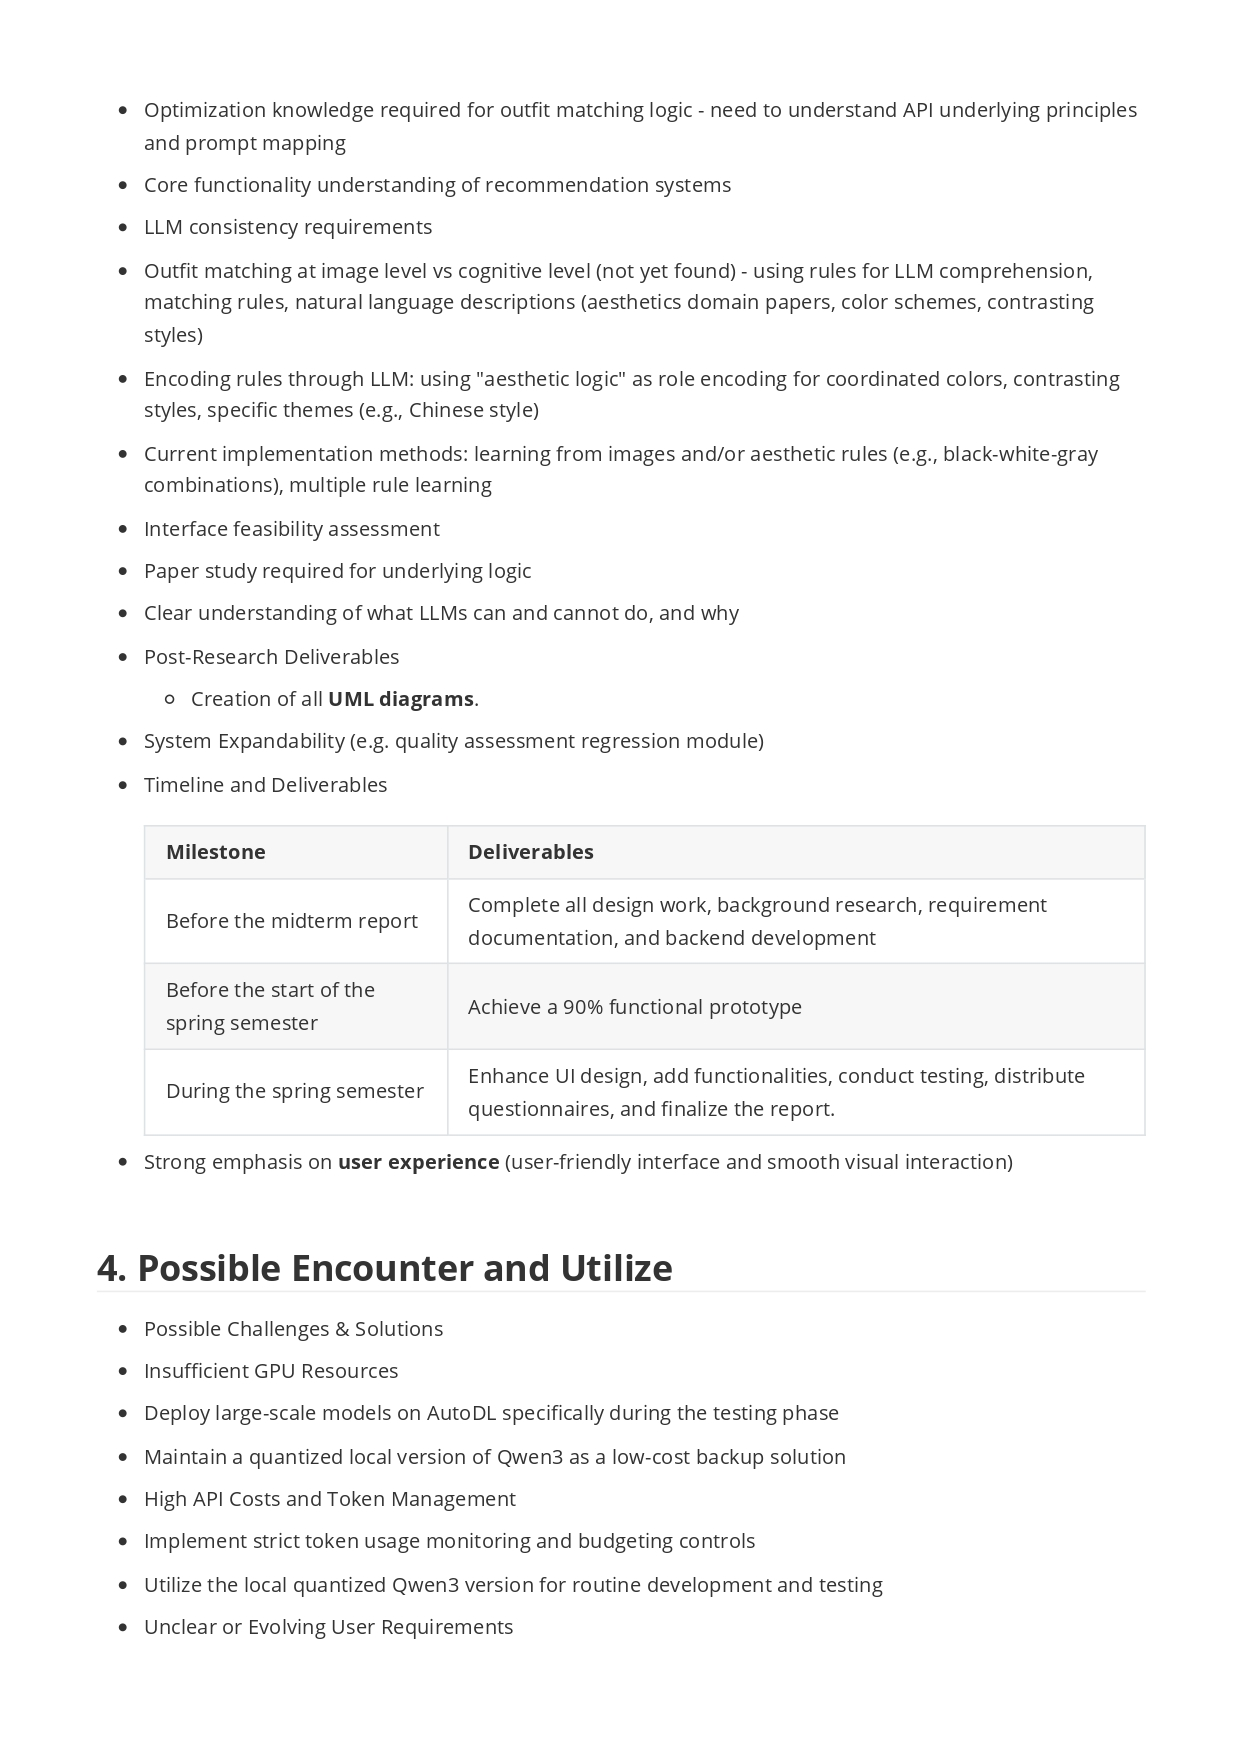
\includegraphics[width=1.0\textwidth]{images/appendix/4th_Formal_Meeting_Minutes_2025-11-05_page-0003.jpg}
\end{figure}
\begin{figure}[H]
    \centering
    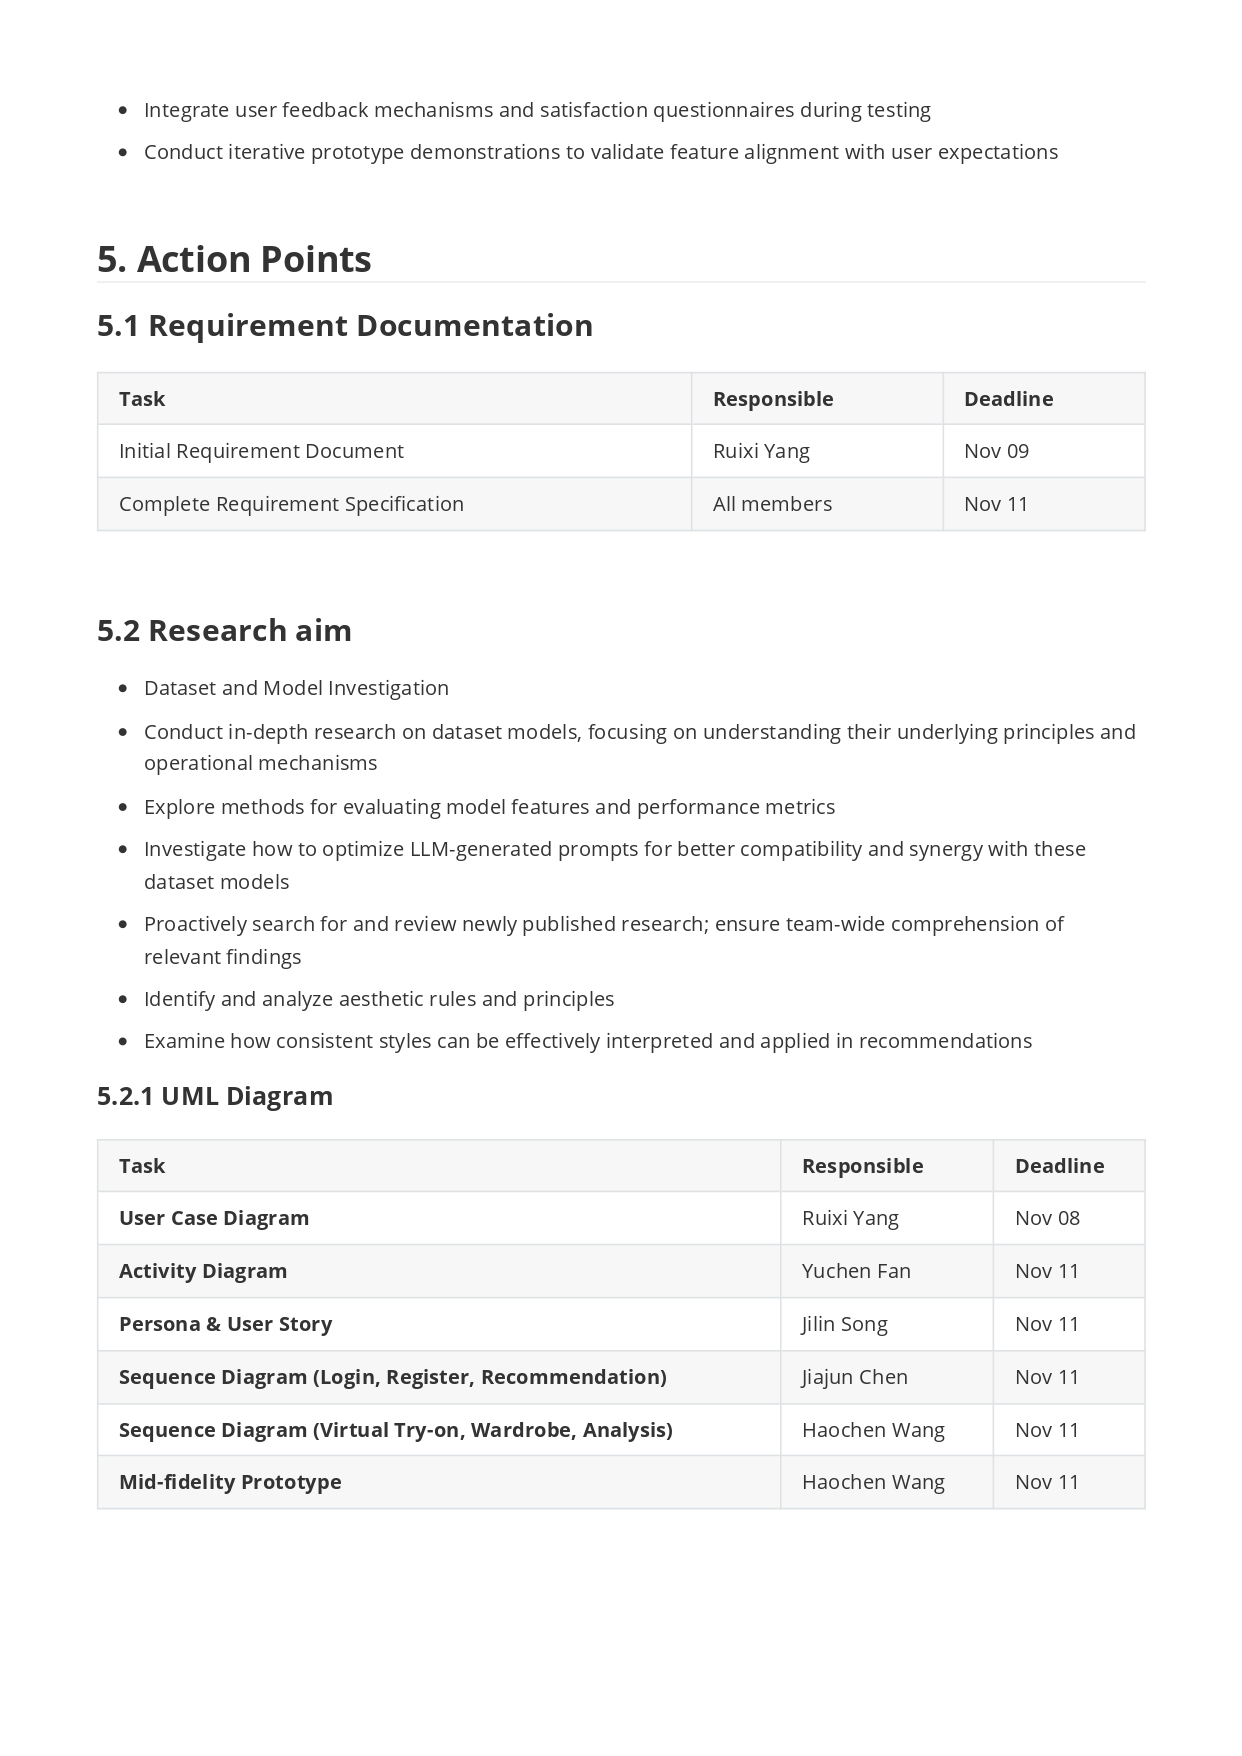
\includegraphics[width=1.0\textwidth]{images/appendix/4th_Formal_Meeting_Minutes_2025-11-05_page-0004.jpg}
\end{figure}
\begin{figure}[H]
    \centering
    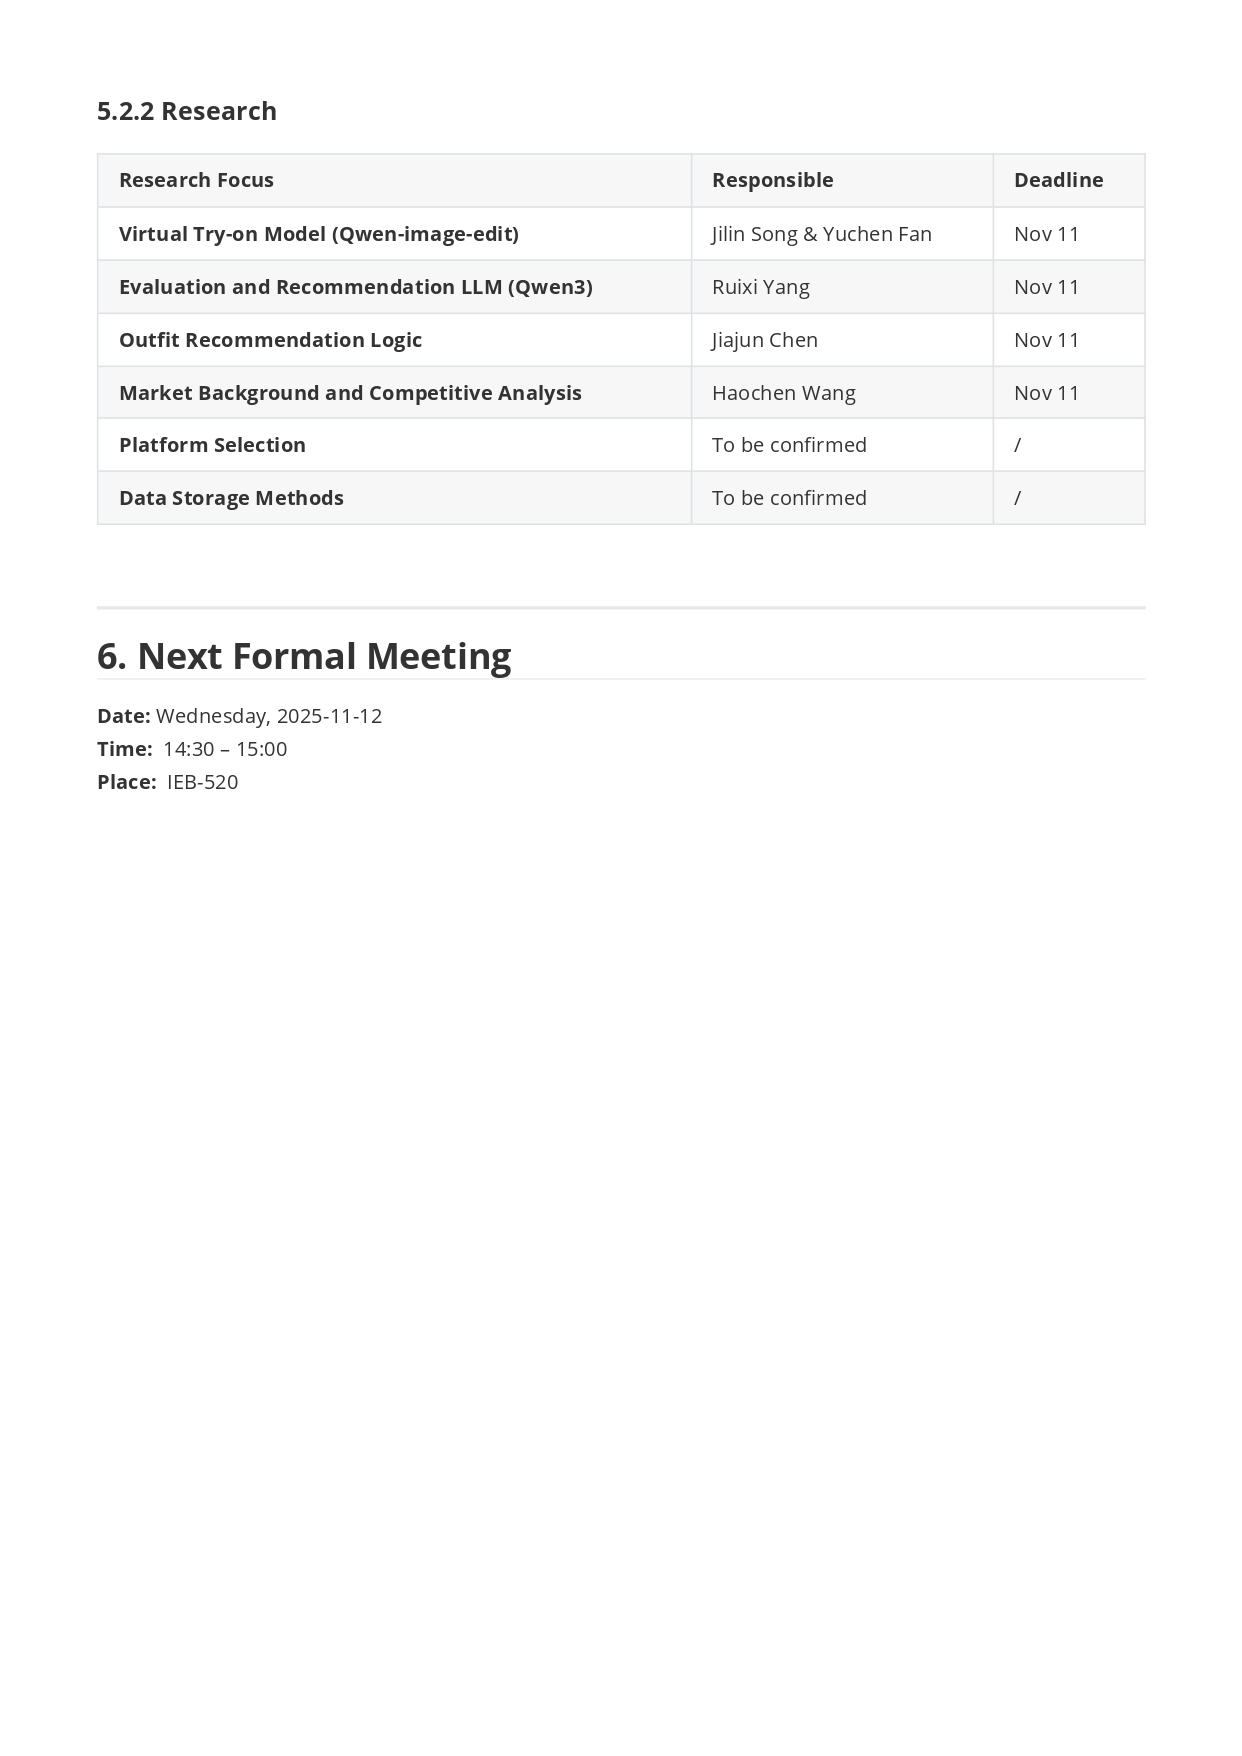
\includegraphics[width=1.0\textwidth]{images/appendix/4th_Formal_Meeting_Minutes_2025-11-05_page-0005.jpg}
\end{figure}


\section{4th Informal Meeting Minutes (2025-11-08)}
\begin{figure}[H]
    \centering
    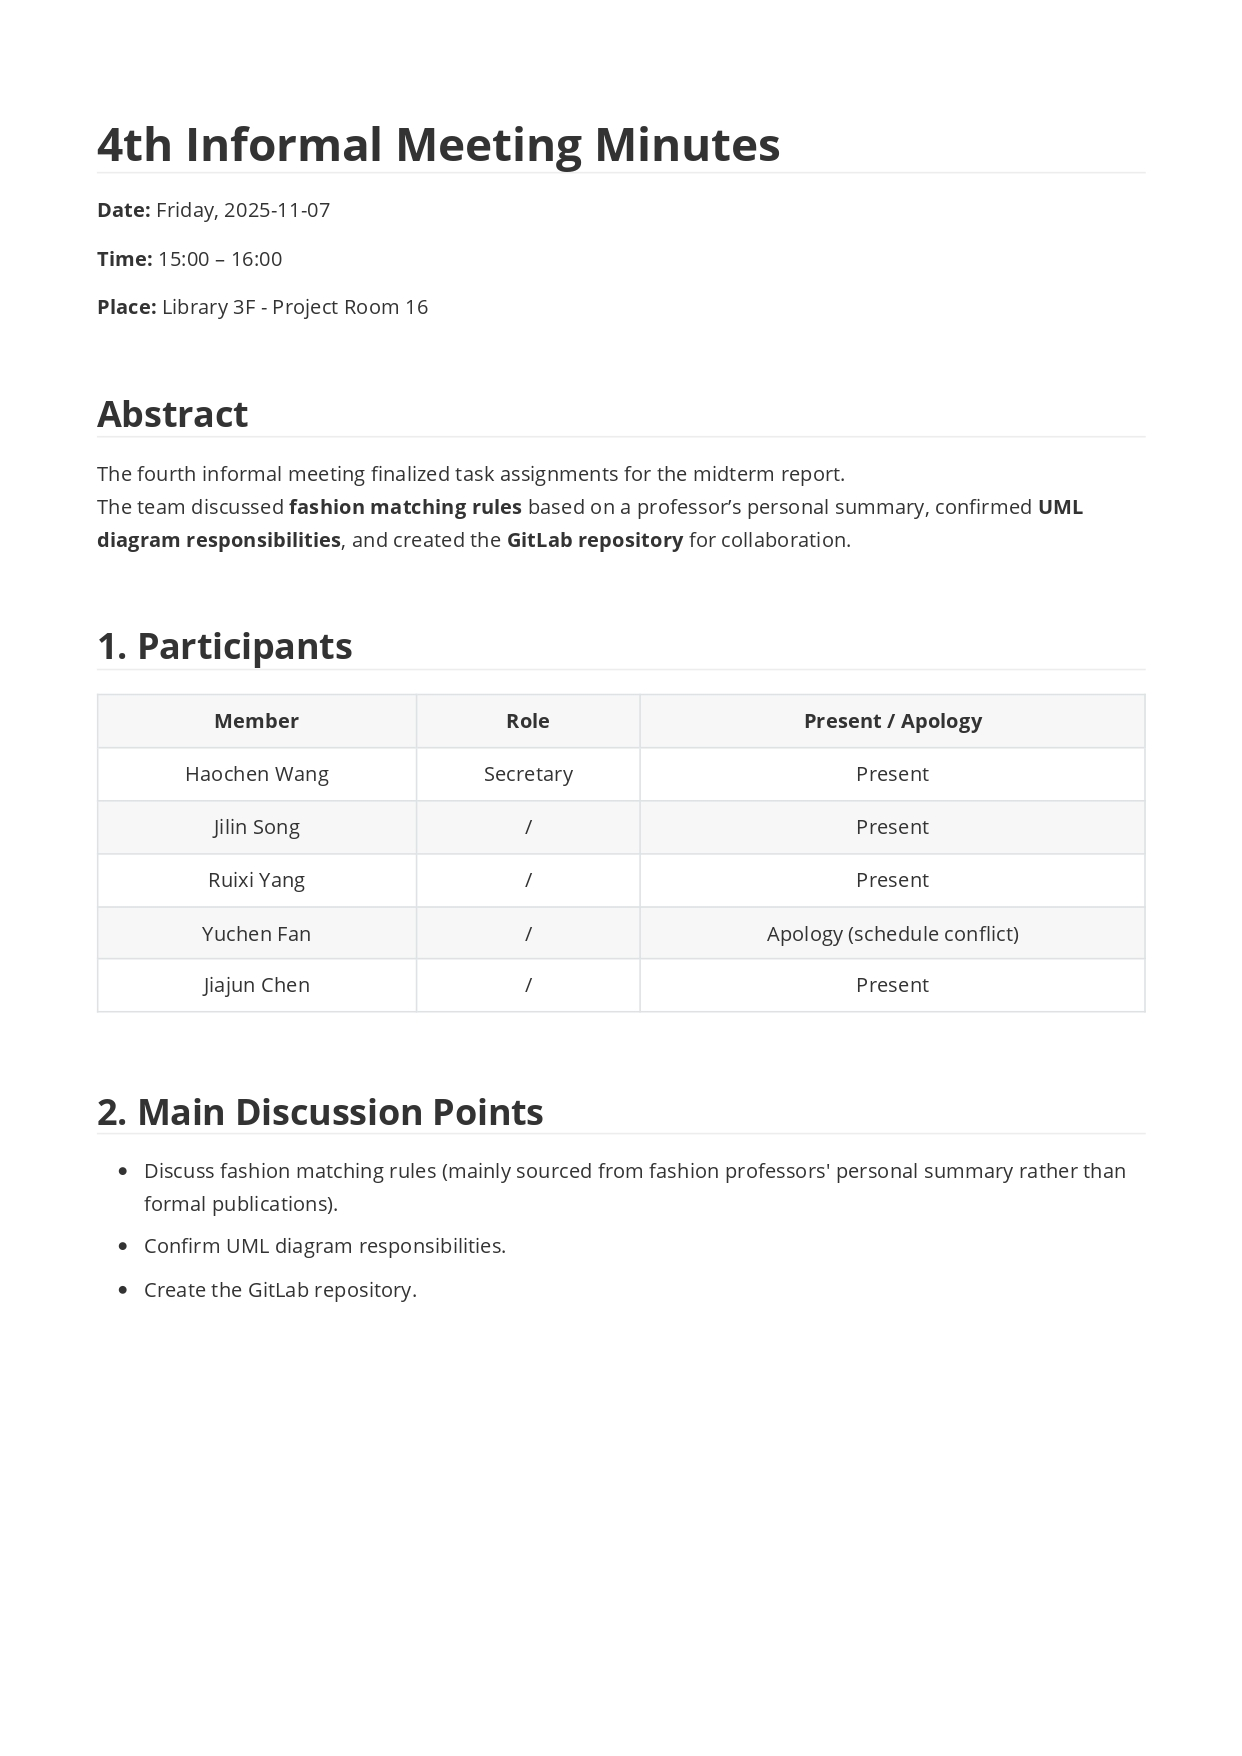
\includegraphics[width=1.0\textwidth]{images/appendix/4th_Informal_Meeting_Minutes_2025-11-08_page-0001.jpg}
\end{figure}
\begin{figure}[H]
    \centering
    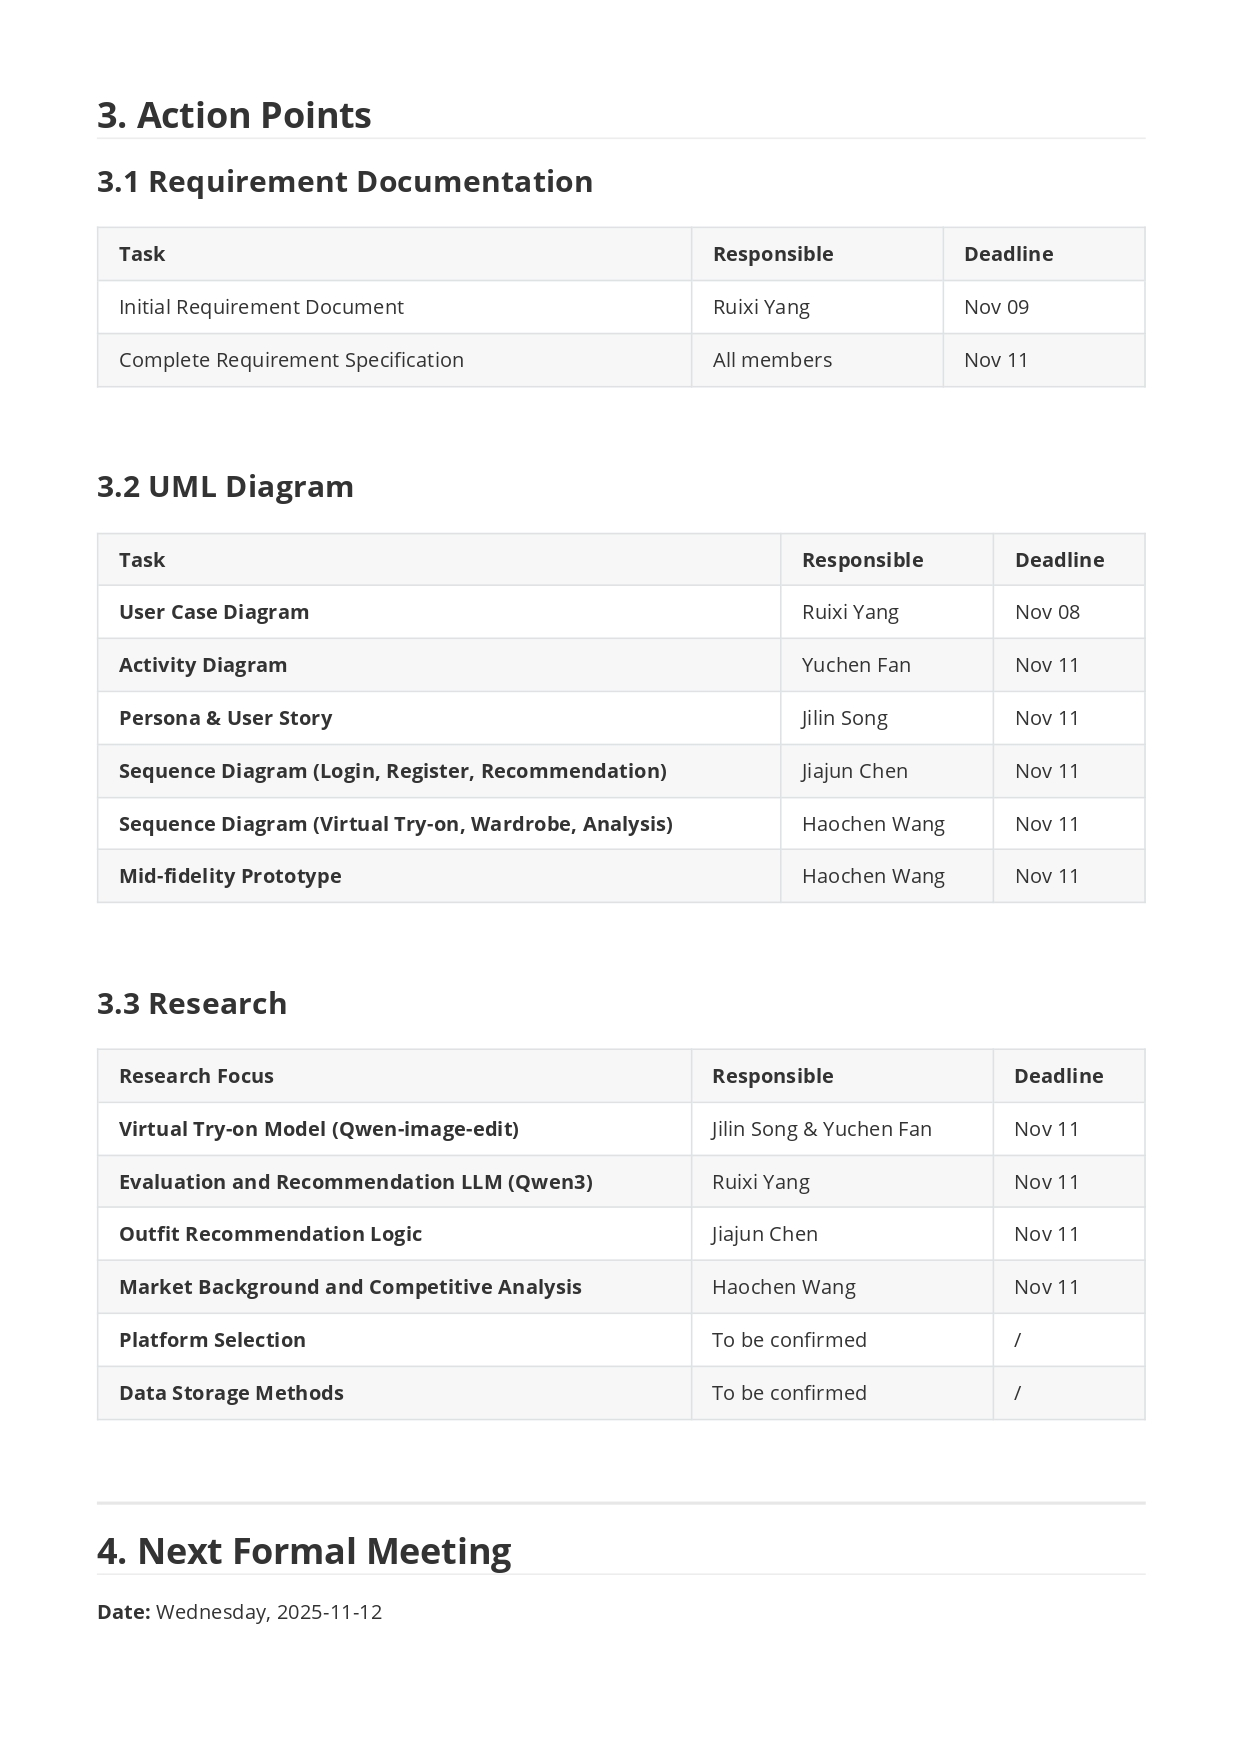
\includegraphics[width=1.0\textwidth]{images/appendix/4th_Informal_Meeting_Minutes_2025-11-08_page-0002.jpg}
\end{figure}


\section{5th Formal Meeting Minutes (2025-11-12)}
\begin{figure}[H]
    \centering
    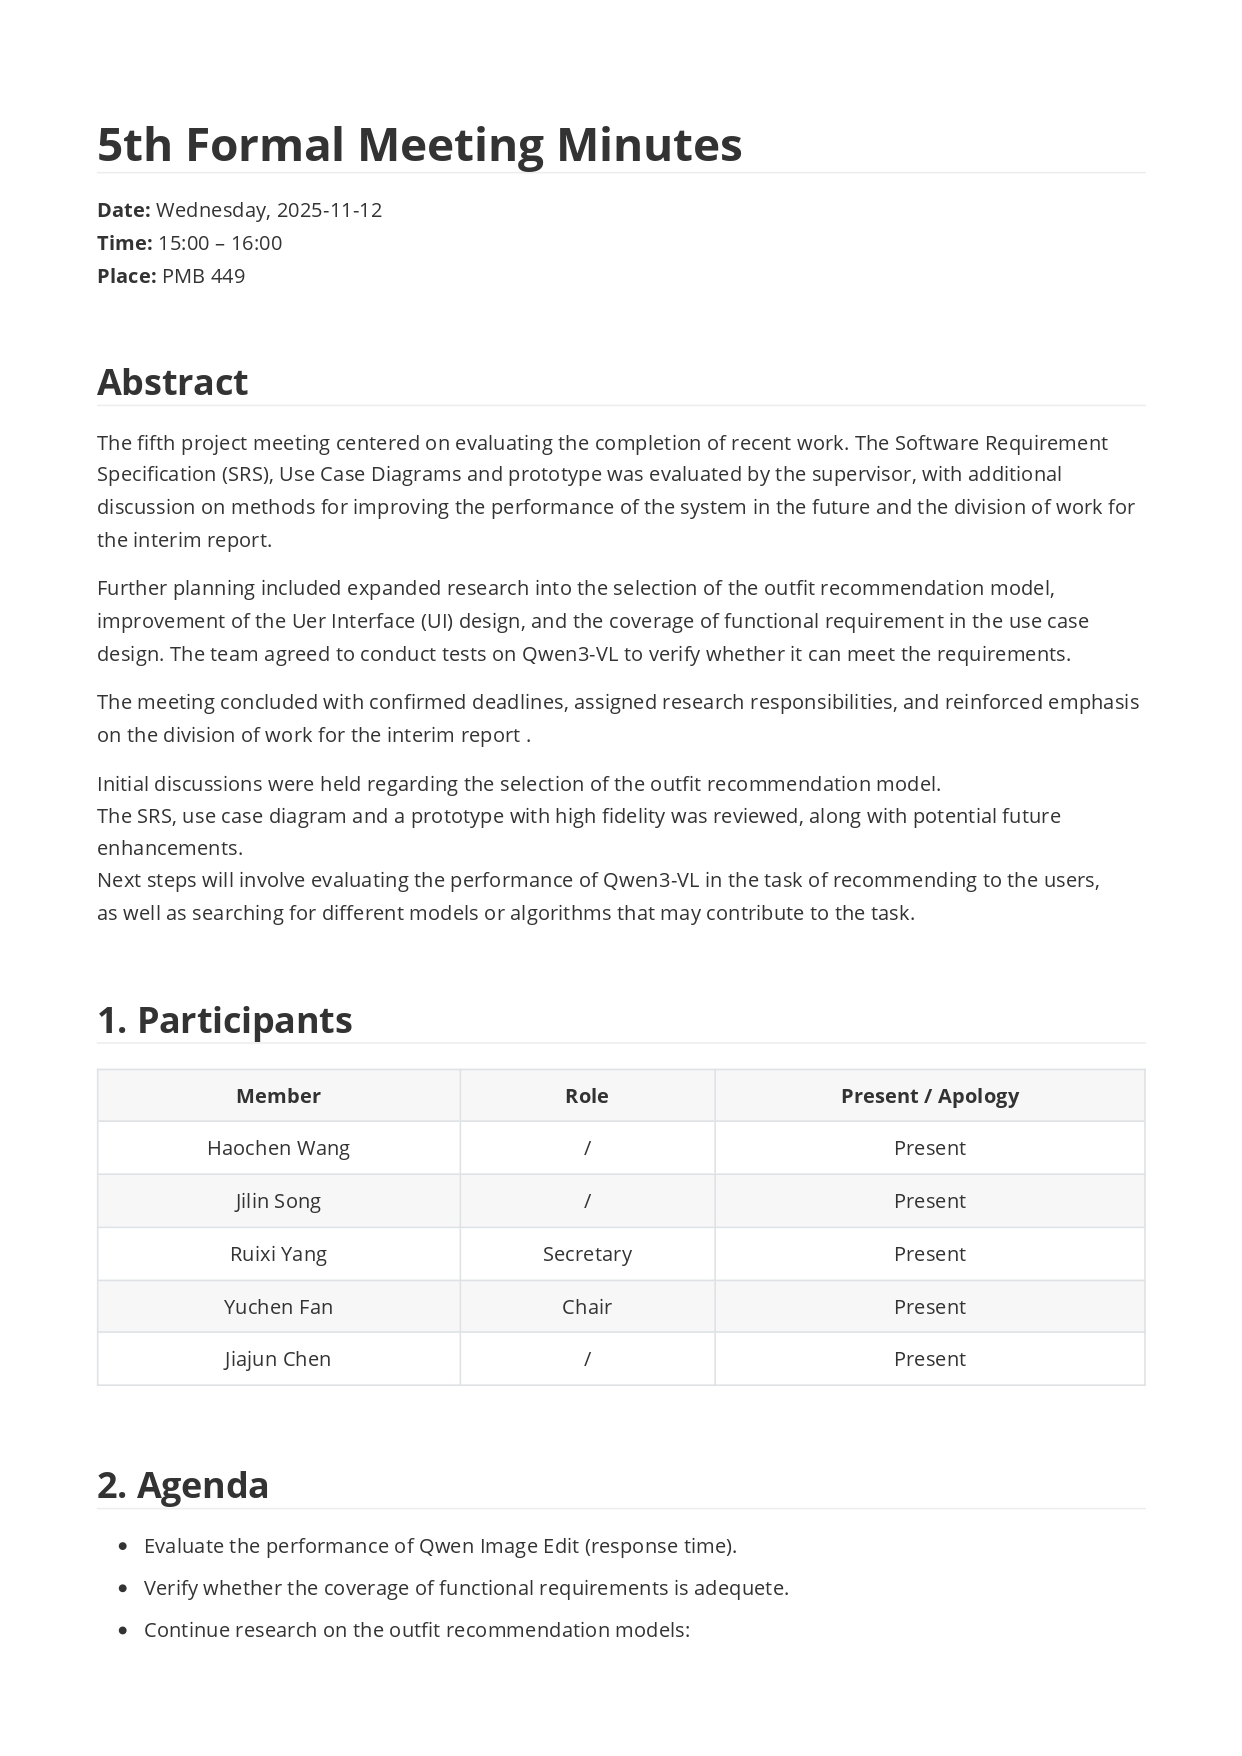
\includegraphics[width=1.0\textwidth]{images/appendix/5th_Formal_Meeting_Minutes_2025-11-12_page-0001.jpg}
\end{figure}
\begin{figure}[H]
    \centering
    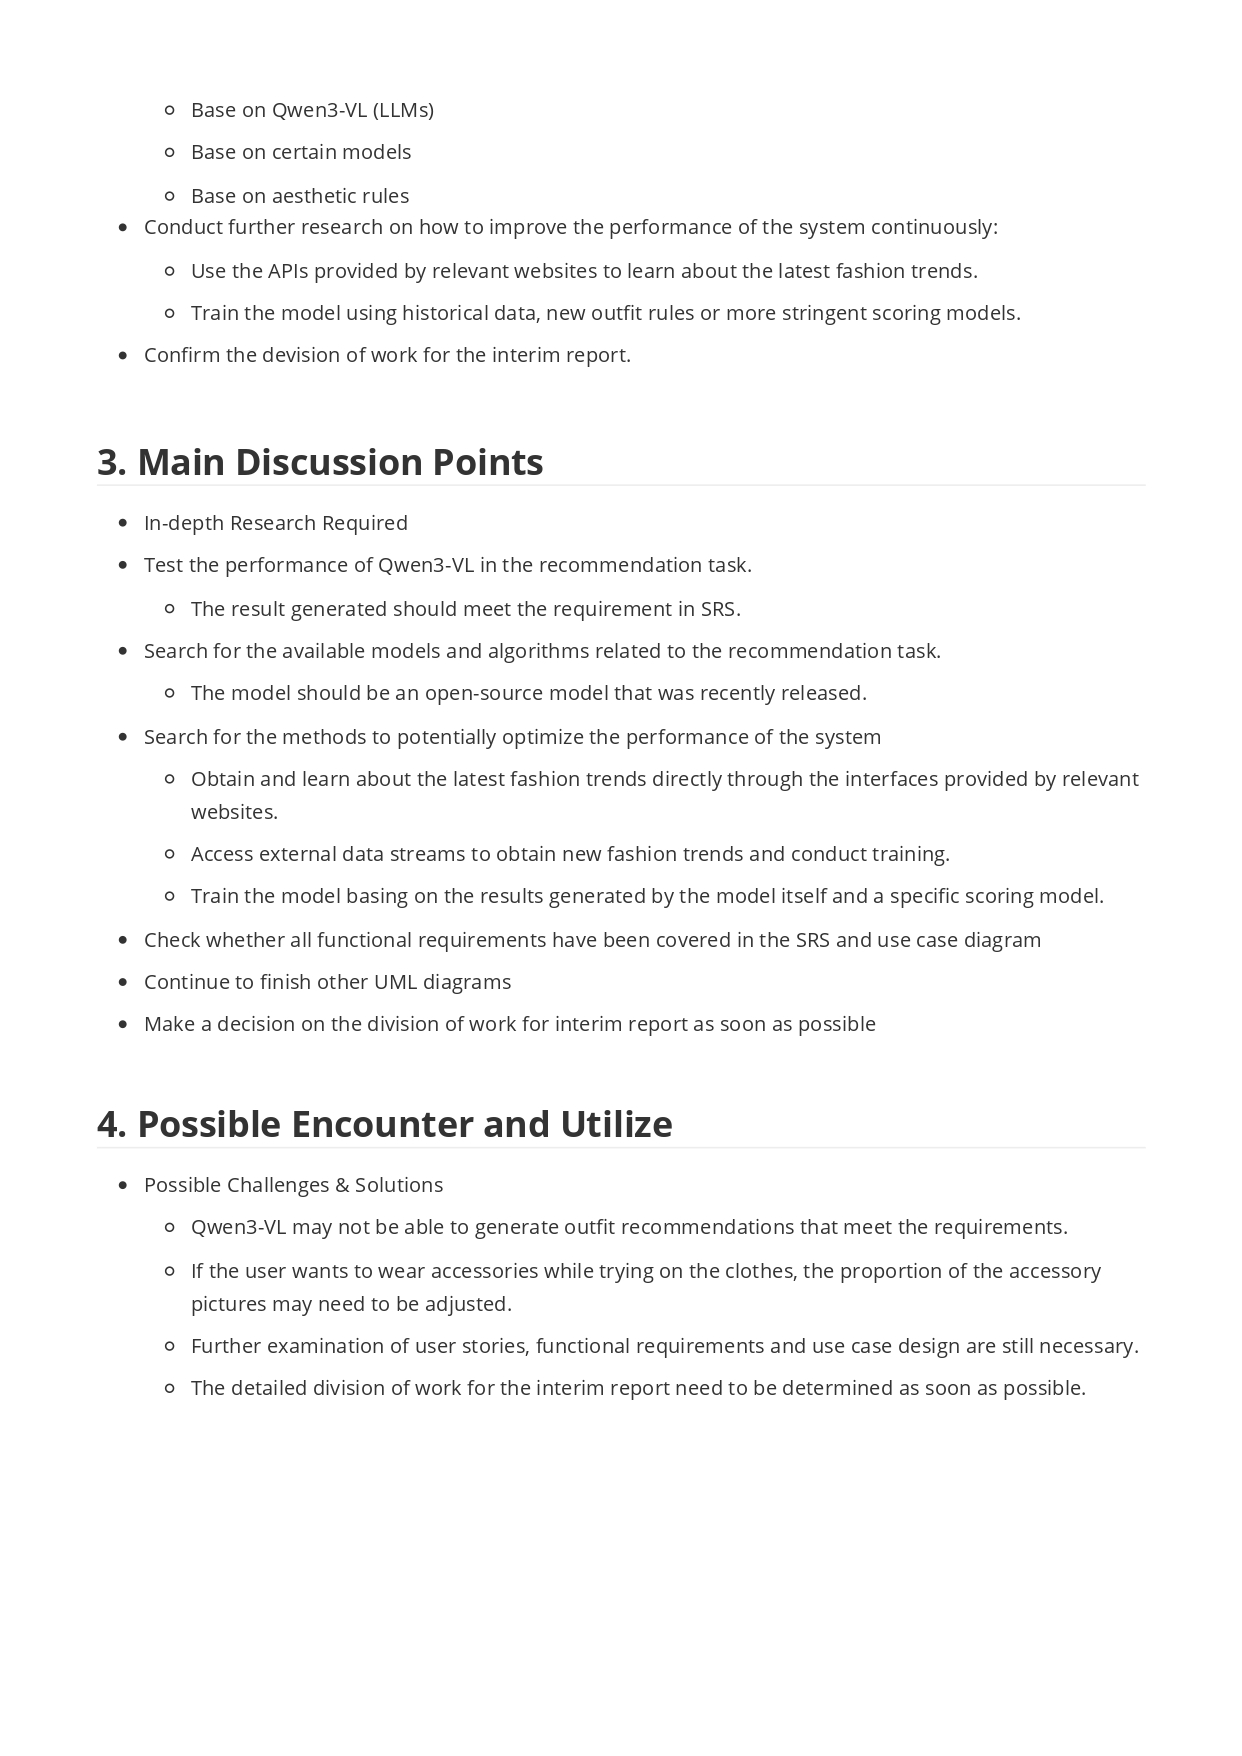
\includegraphics[width=1.0\textwidth]{images/appendix/5th_Formal_Meeting_Minutes_2025-11-12_page-0002.jpg}
\end{figure}
\begin{figure}[H]
    \centering
    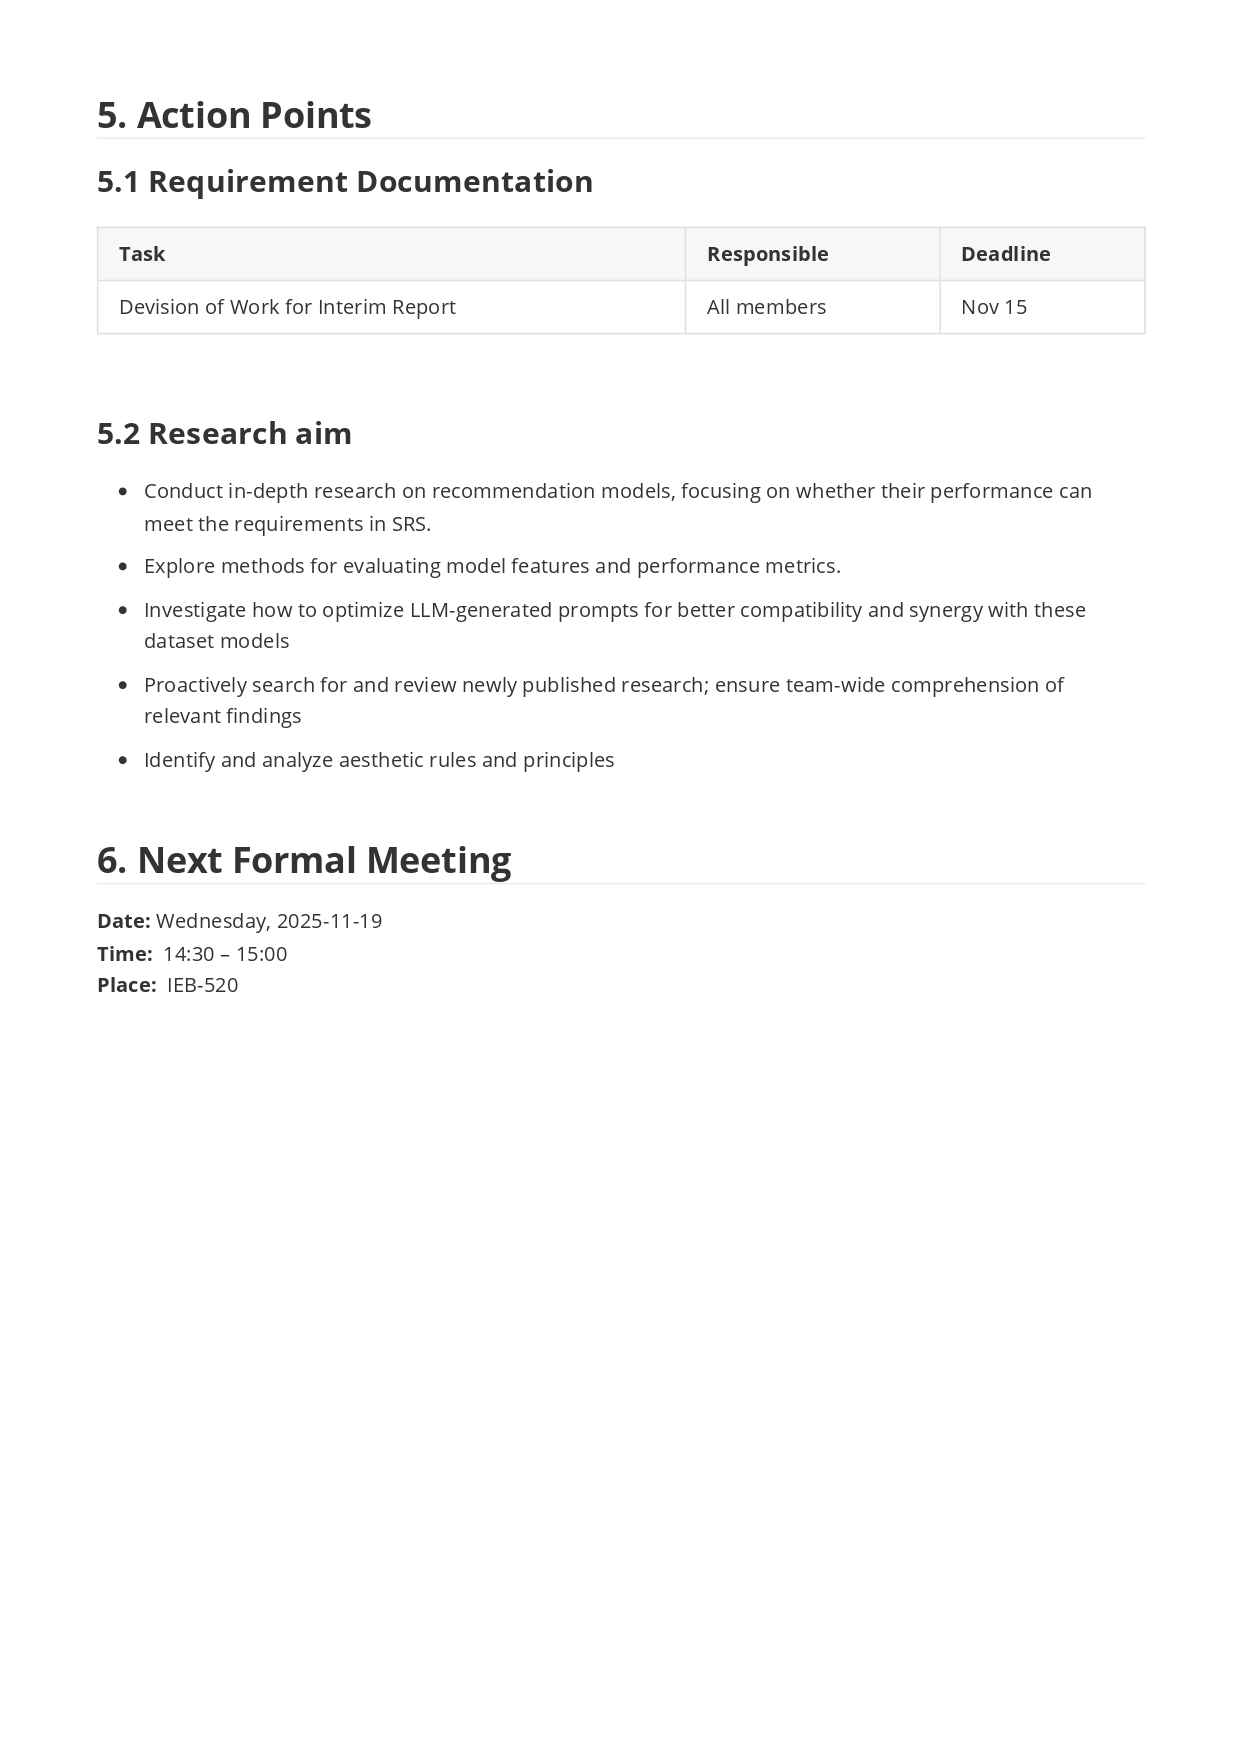
\includegraphics[width=1.0\textwidth]{images/appendix/5th_Formal_Meeting_Minutes_2025-11-12_page-0003.jpg}
\end{figure}


\section{6th Formal Meeting Minutes (2025-11-26)}
\begin{figure}[H]
    \centering
    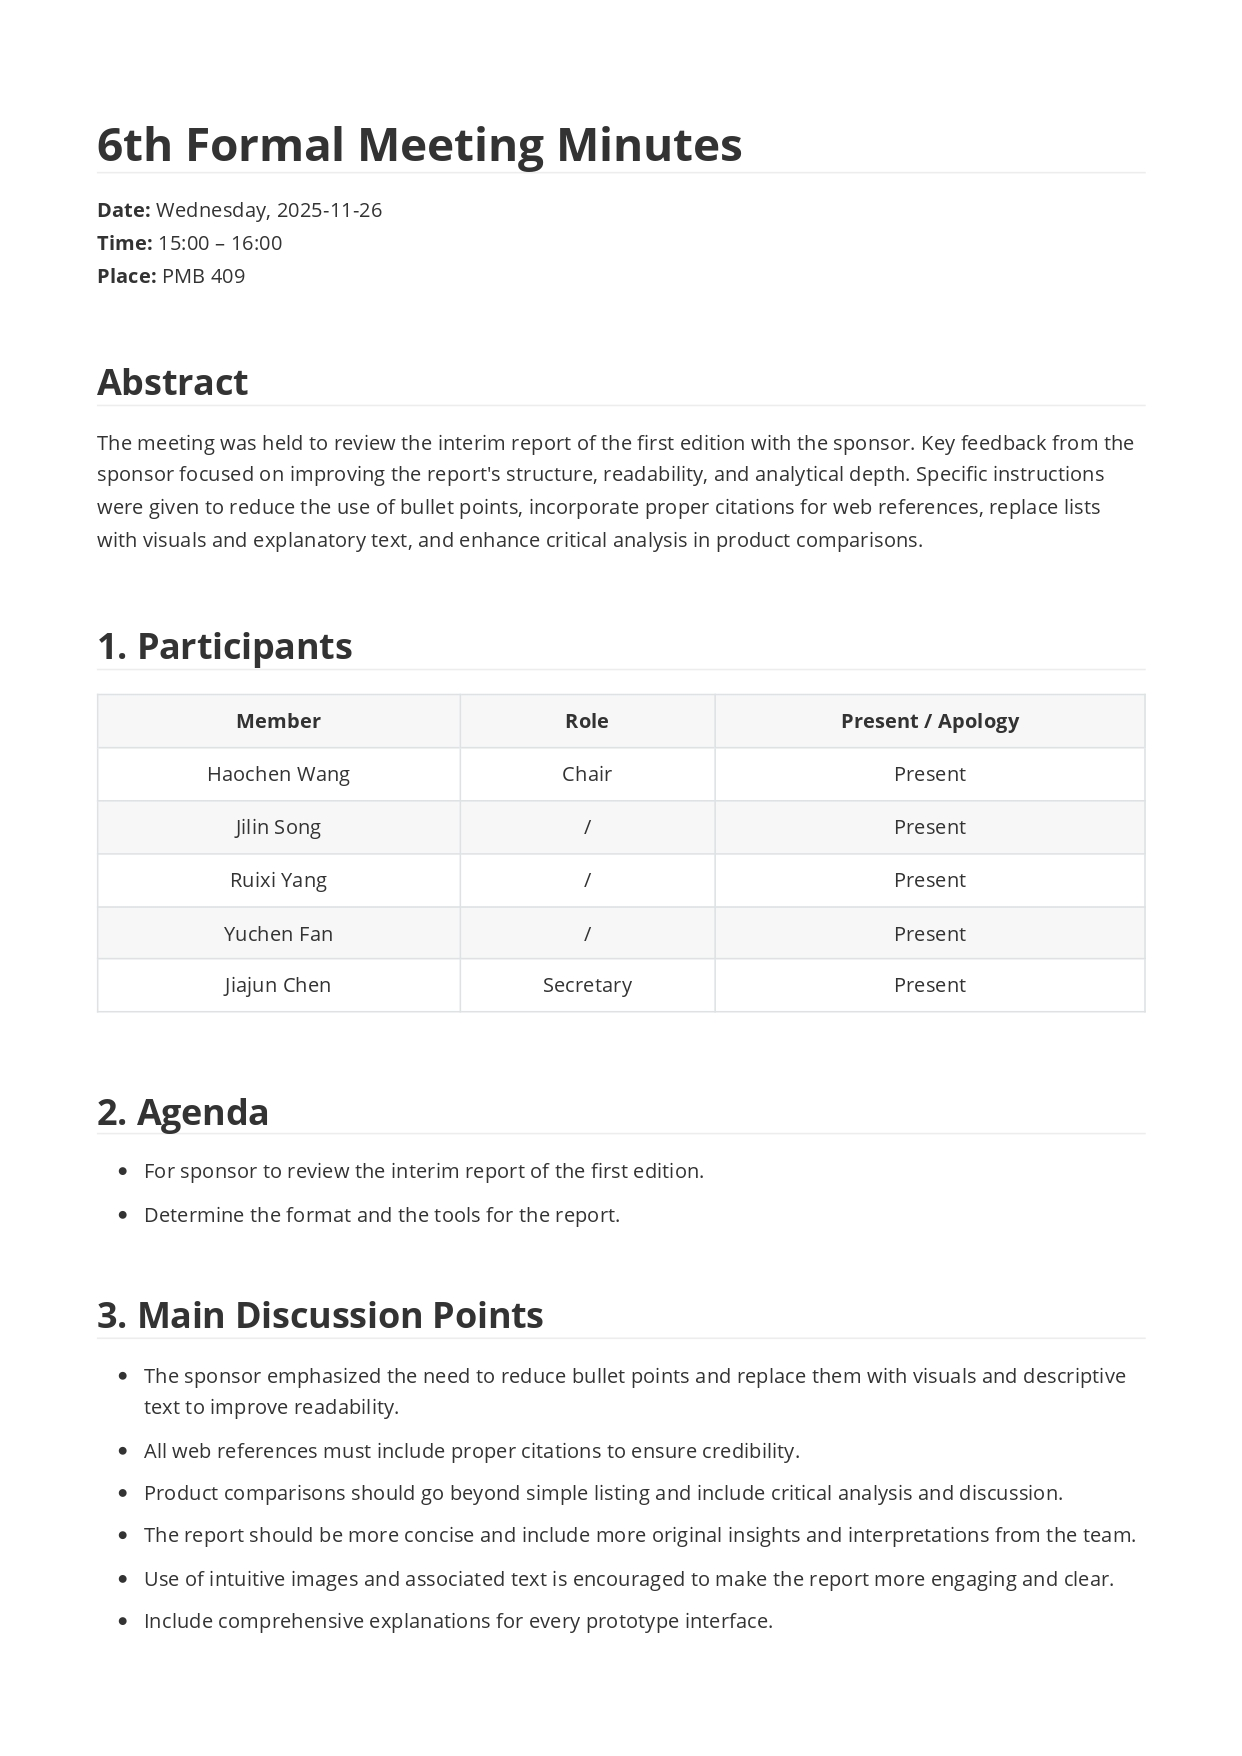
\includegraphics[width=1.0\textwidth]{images/appendix/6th_Formal_Meeting_Minutes_2025-11-26_page-0001.jpg}
\end{figure}
\begin{figure}[H]
    \centering
    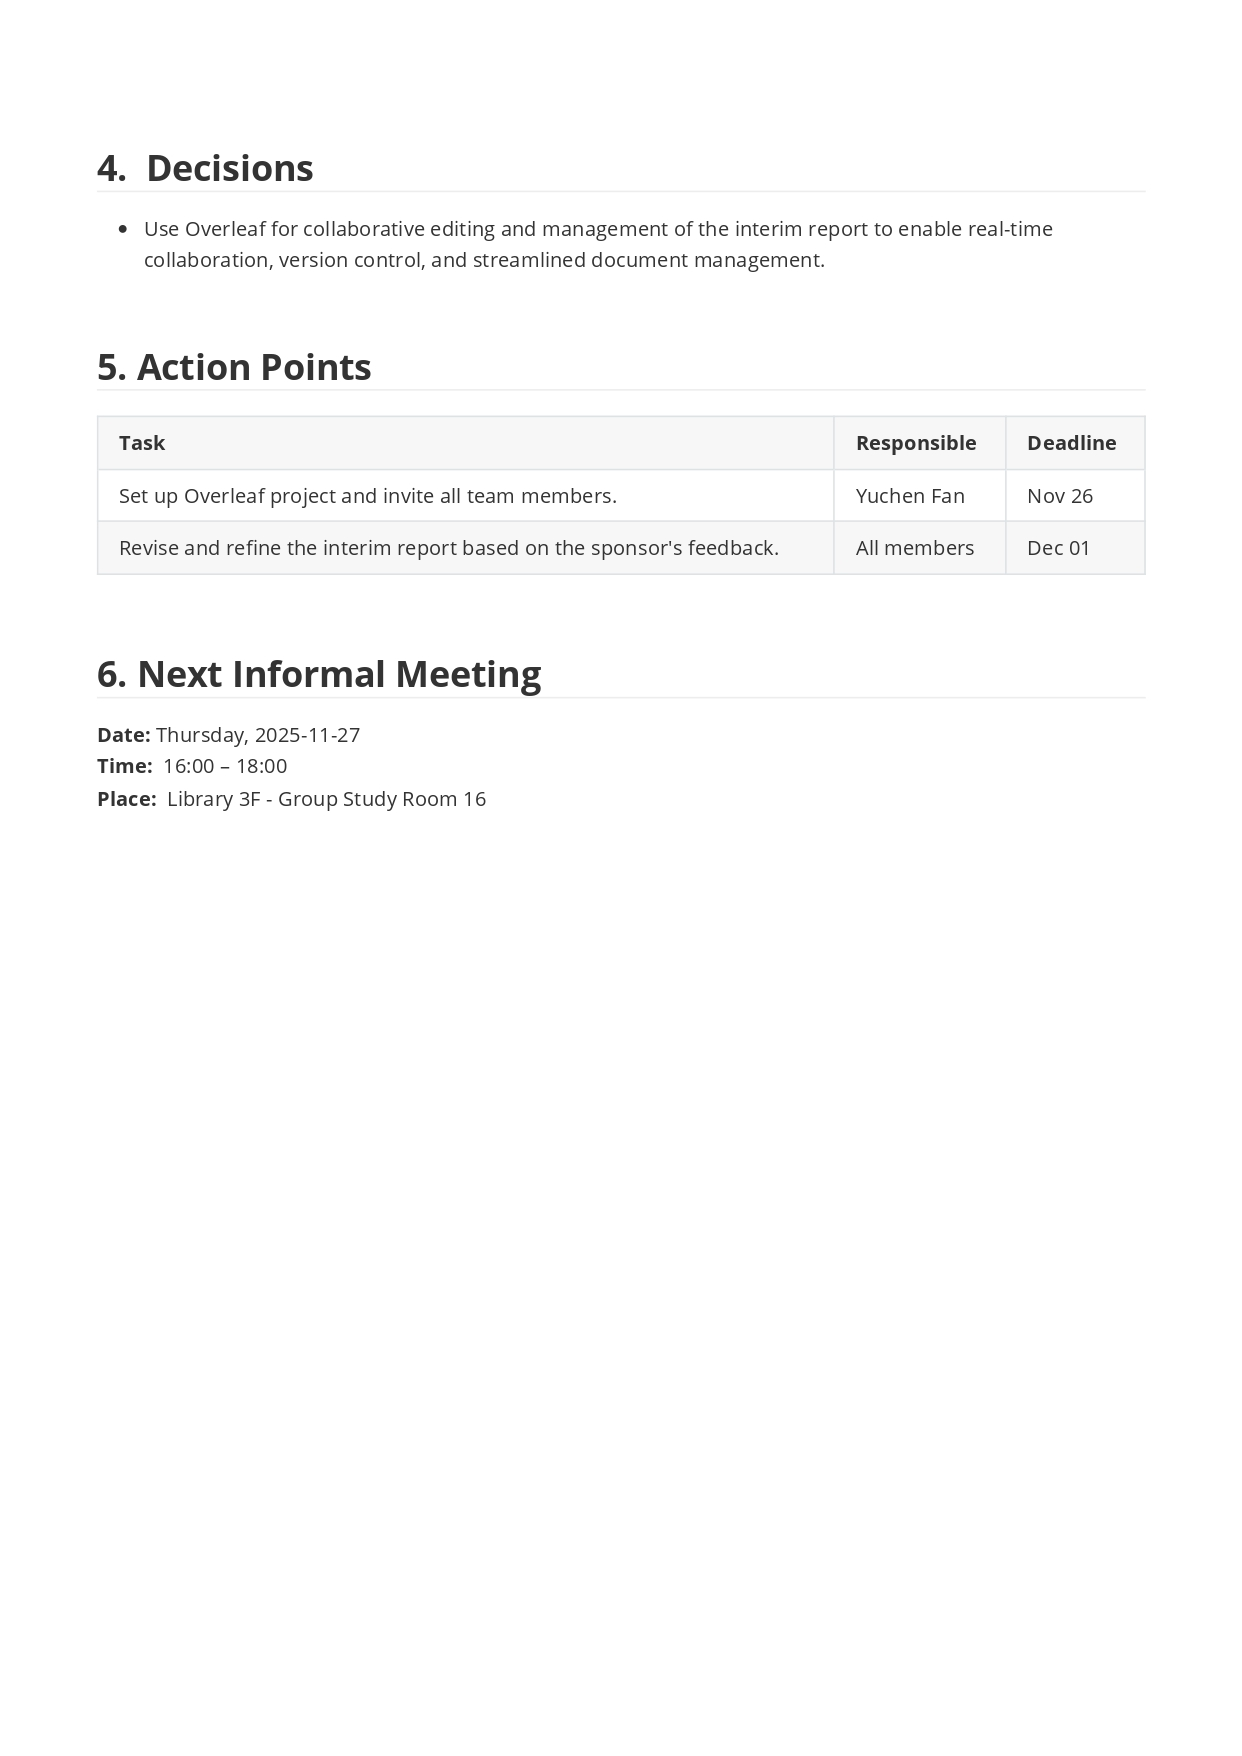
\includegraphics[width=1.0\textwidth]{images/appendix/6th_Formal_Meeting_Minutes_2025-11-26_page-0002.jpg}
\end{figure}


\section{7th Formal Meeting Minutes (2026-01-20)}
\begin{figure}[H]
    \centering
    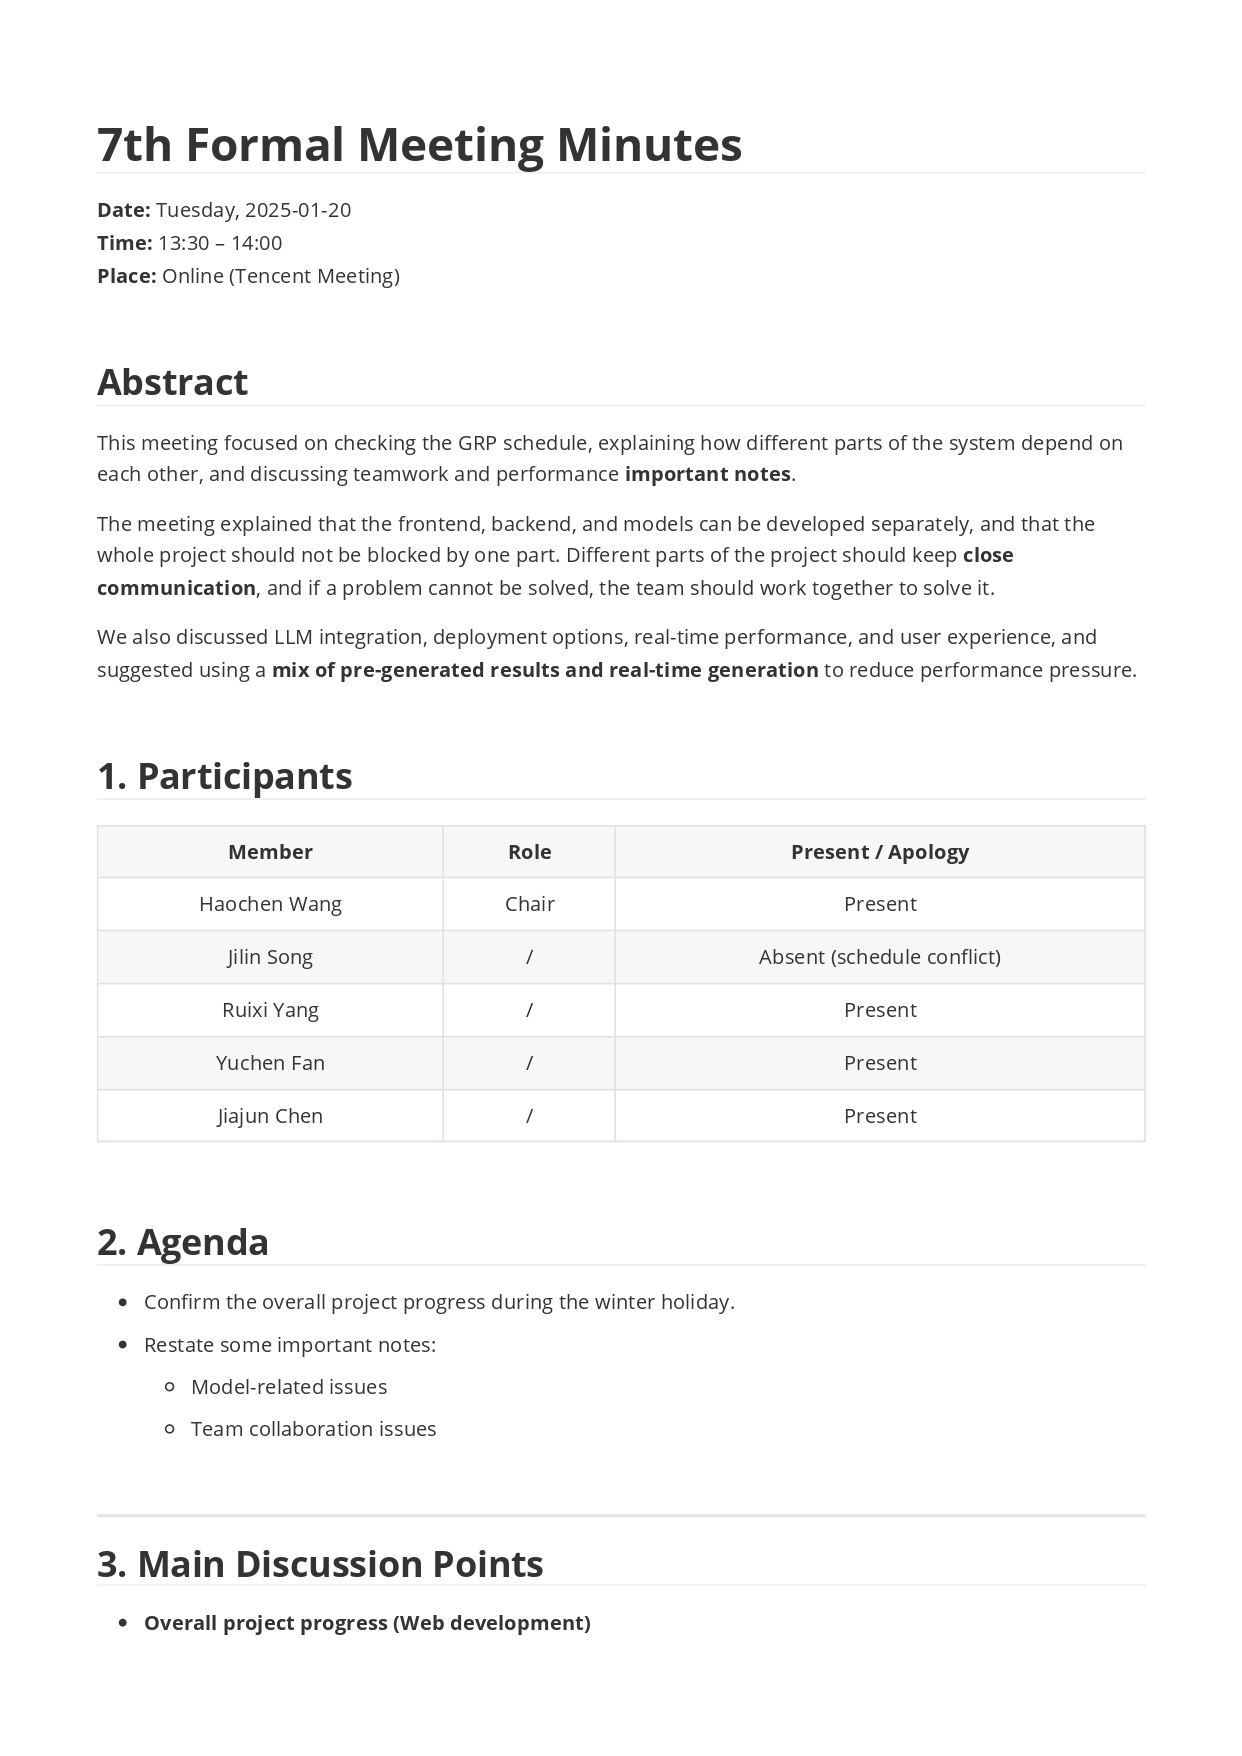
\includegraphics[width=1.0\textwidth]{images/appendix/7th_Formal_Meeting_Minutes_2026-01-20_page-0001.jpg}
\end{figure}
\begin{figure}[H]
    \centering
    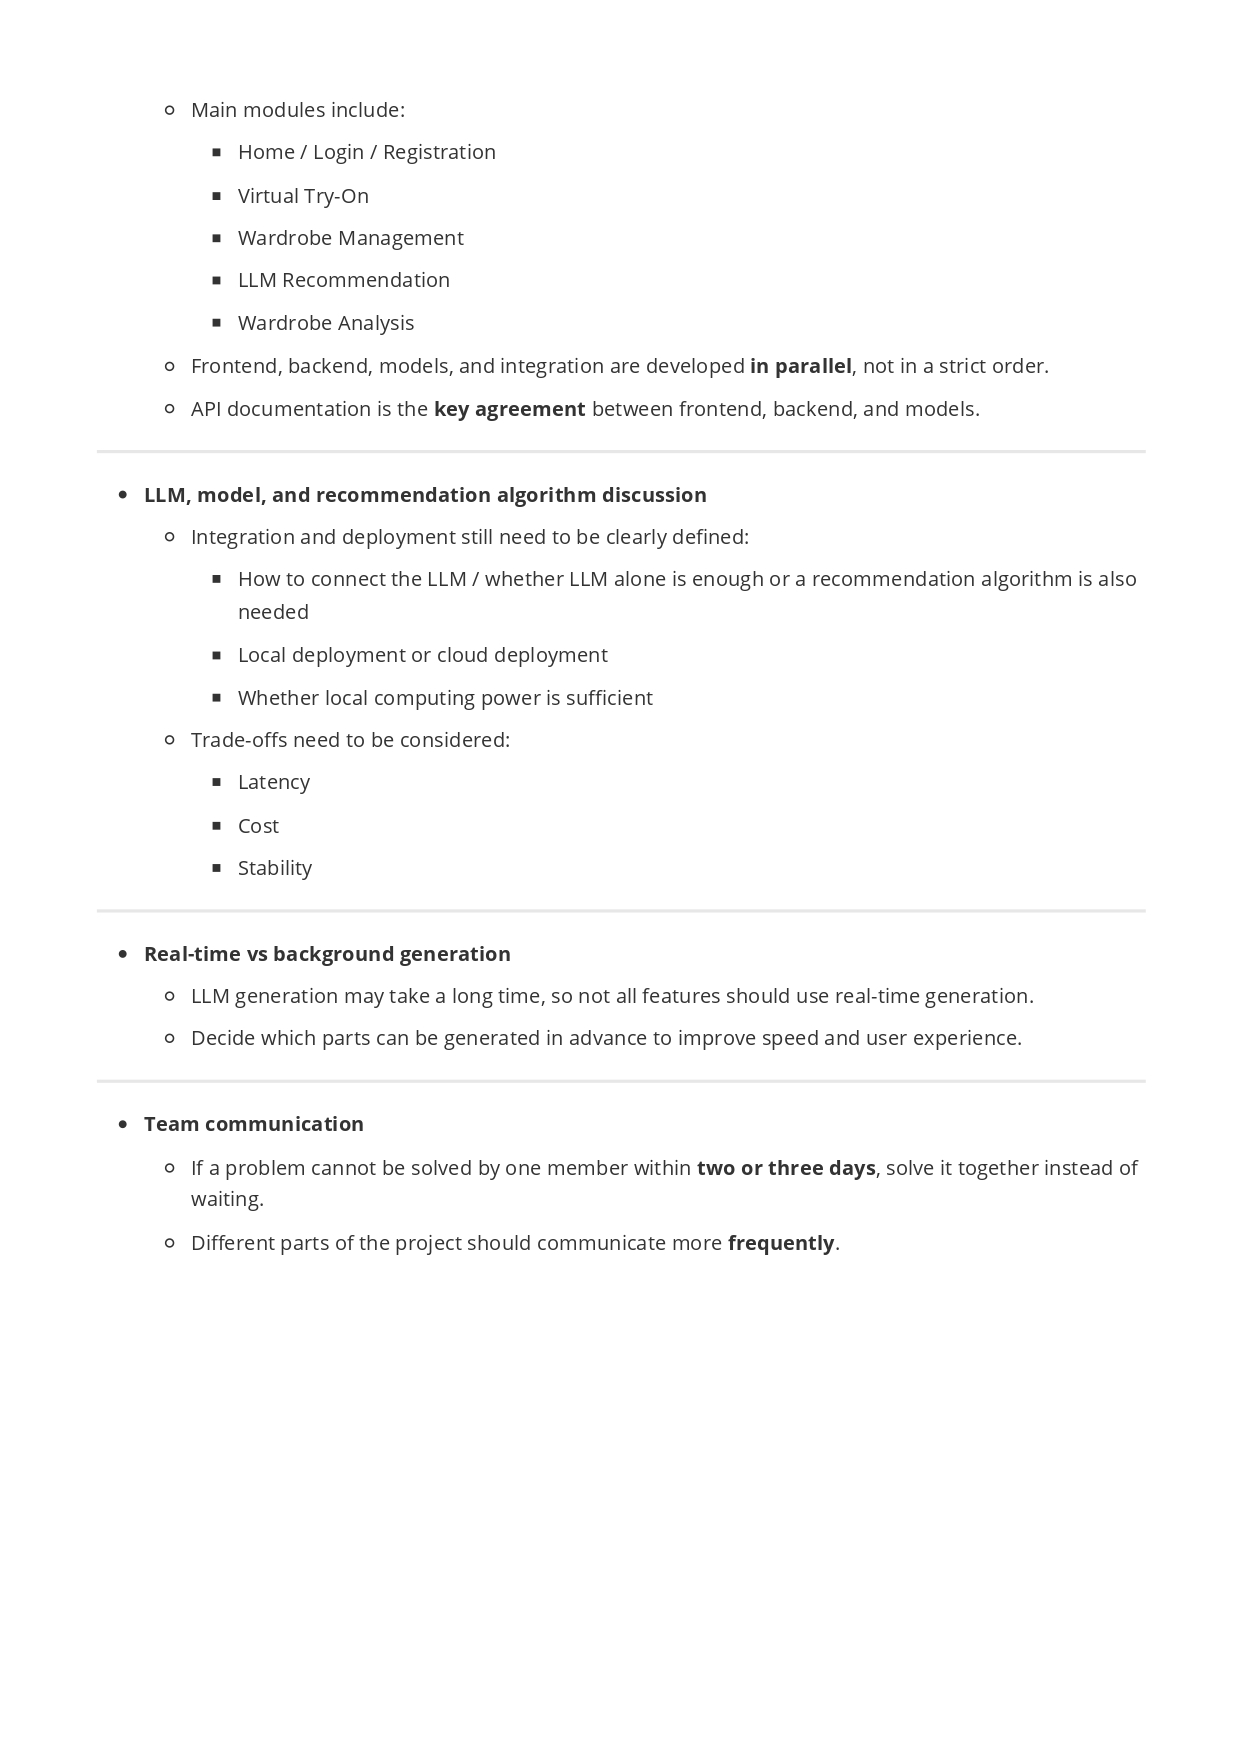
\includegraphics[width=1.0\textwidth]{images/appendix/7th_Formal_Meeting_Minutes_2026-01-20_page-0002.jpg}
\end{figure}
\begin{figure}[H]
    \centering
    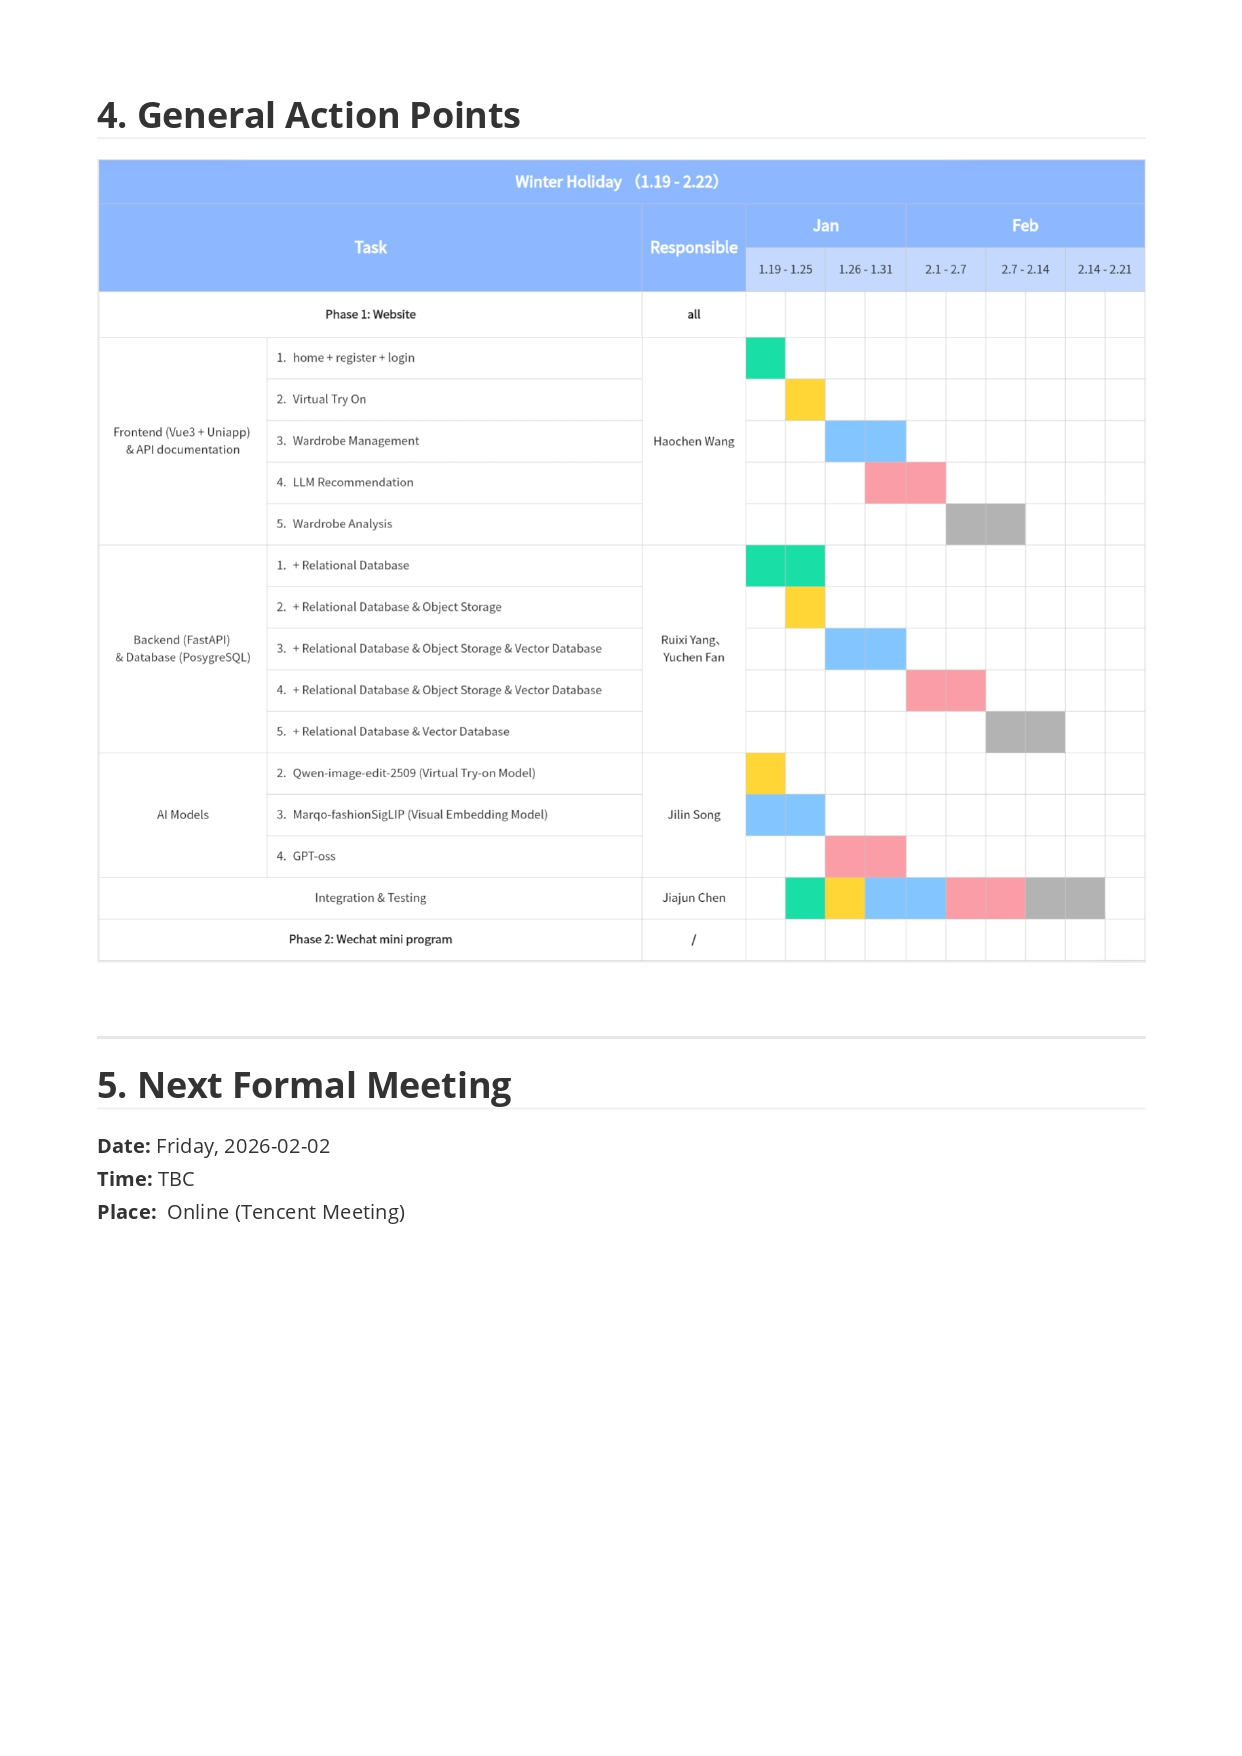
\includegraphics[width=1.0\textwidth]{images/appendix/7th_Formal_Meeting_Minutes_2026-01-20_page-0003.jpg}
\end{figure}


\section{8th Formal Meeting Minutes (2026-02-02)}
\begin{figure}[H]
    \centering
    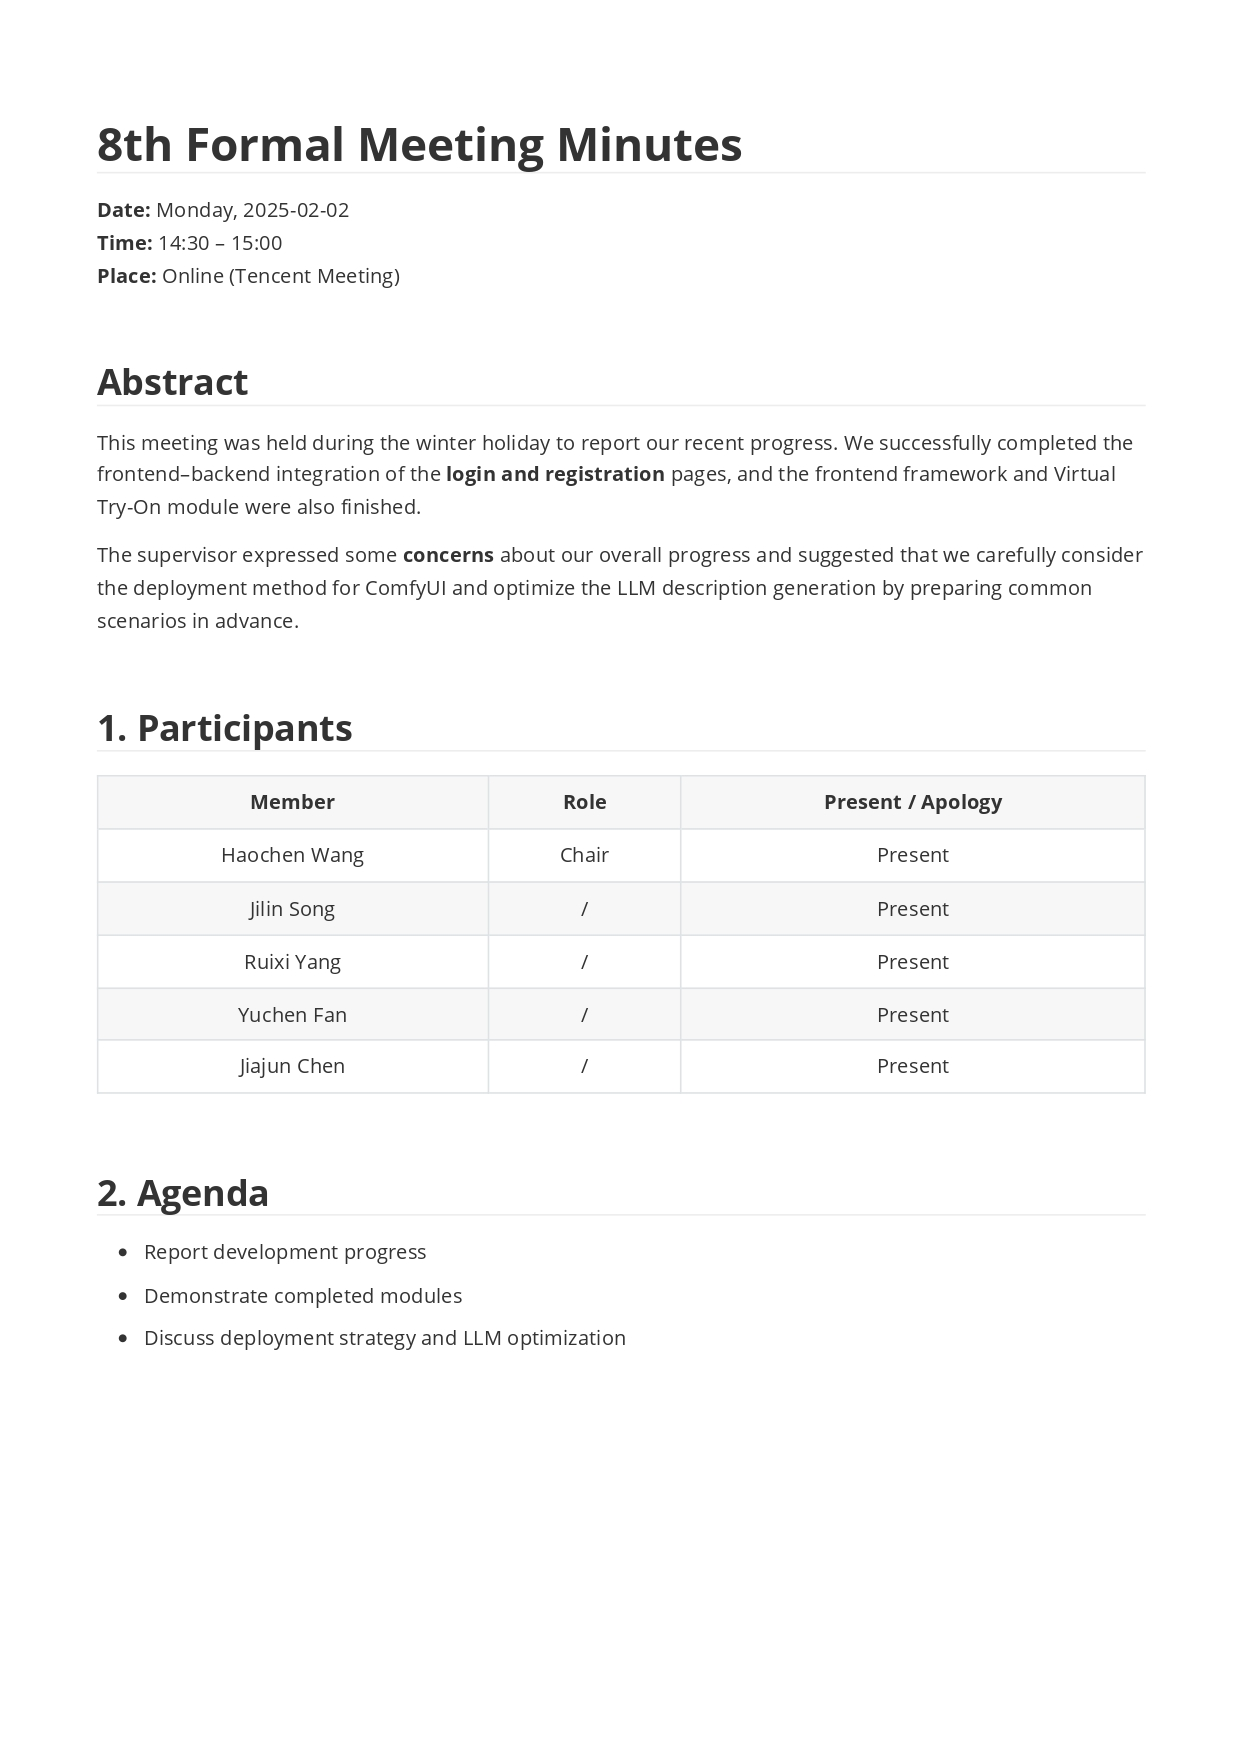
\includegraphics[width=1.0\textwidth]{images/appendix/8th_Formal_Meeting_Minutes_2026-02-02_page-0001.jpg}
\end{figure}
\begin{figure}[H]
    \centering
    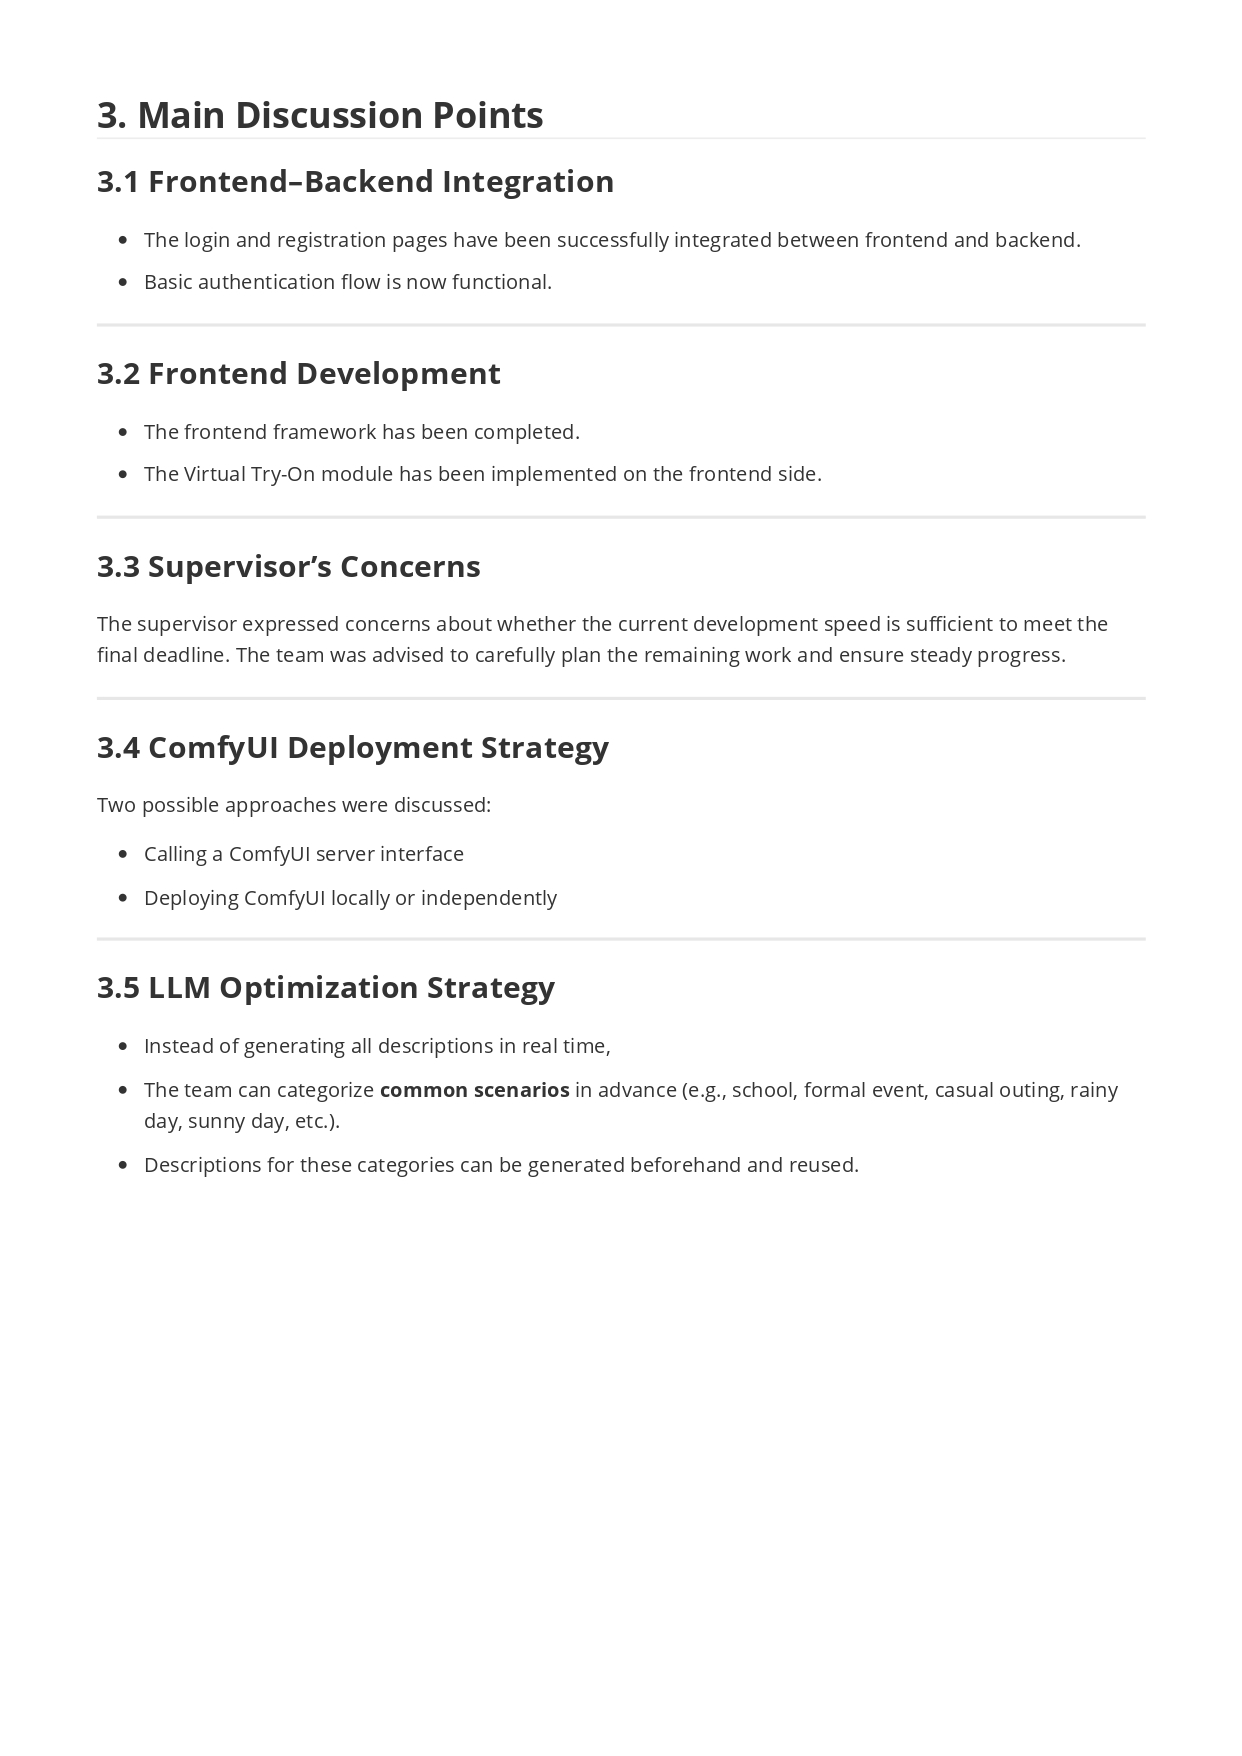
\includegraphics[width=1.0\textwidth]{images/appendix/8th_Formal_Meeting_Minutes_2026-02-02_page-0002.jpg}
\end{figure}
\begin{figure}[H]
    \centering
    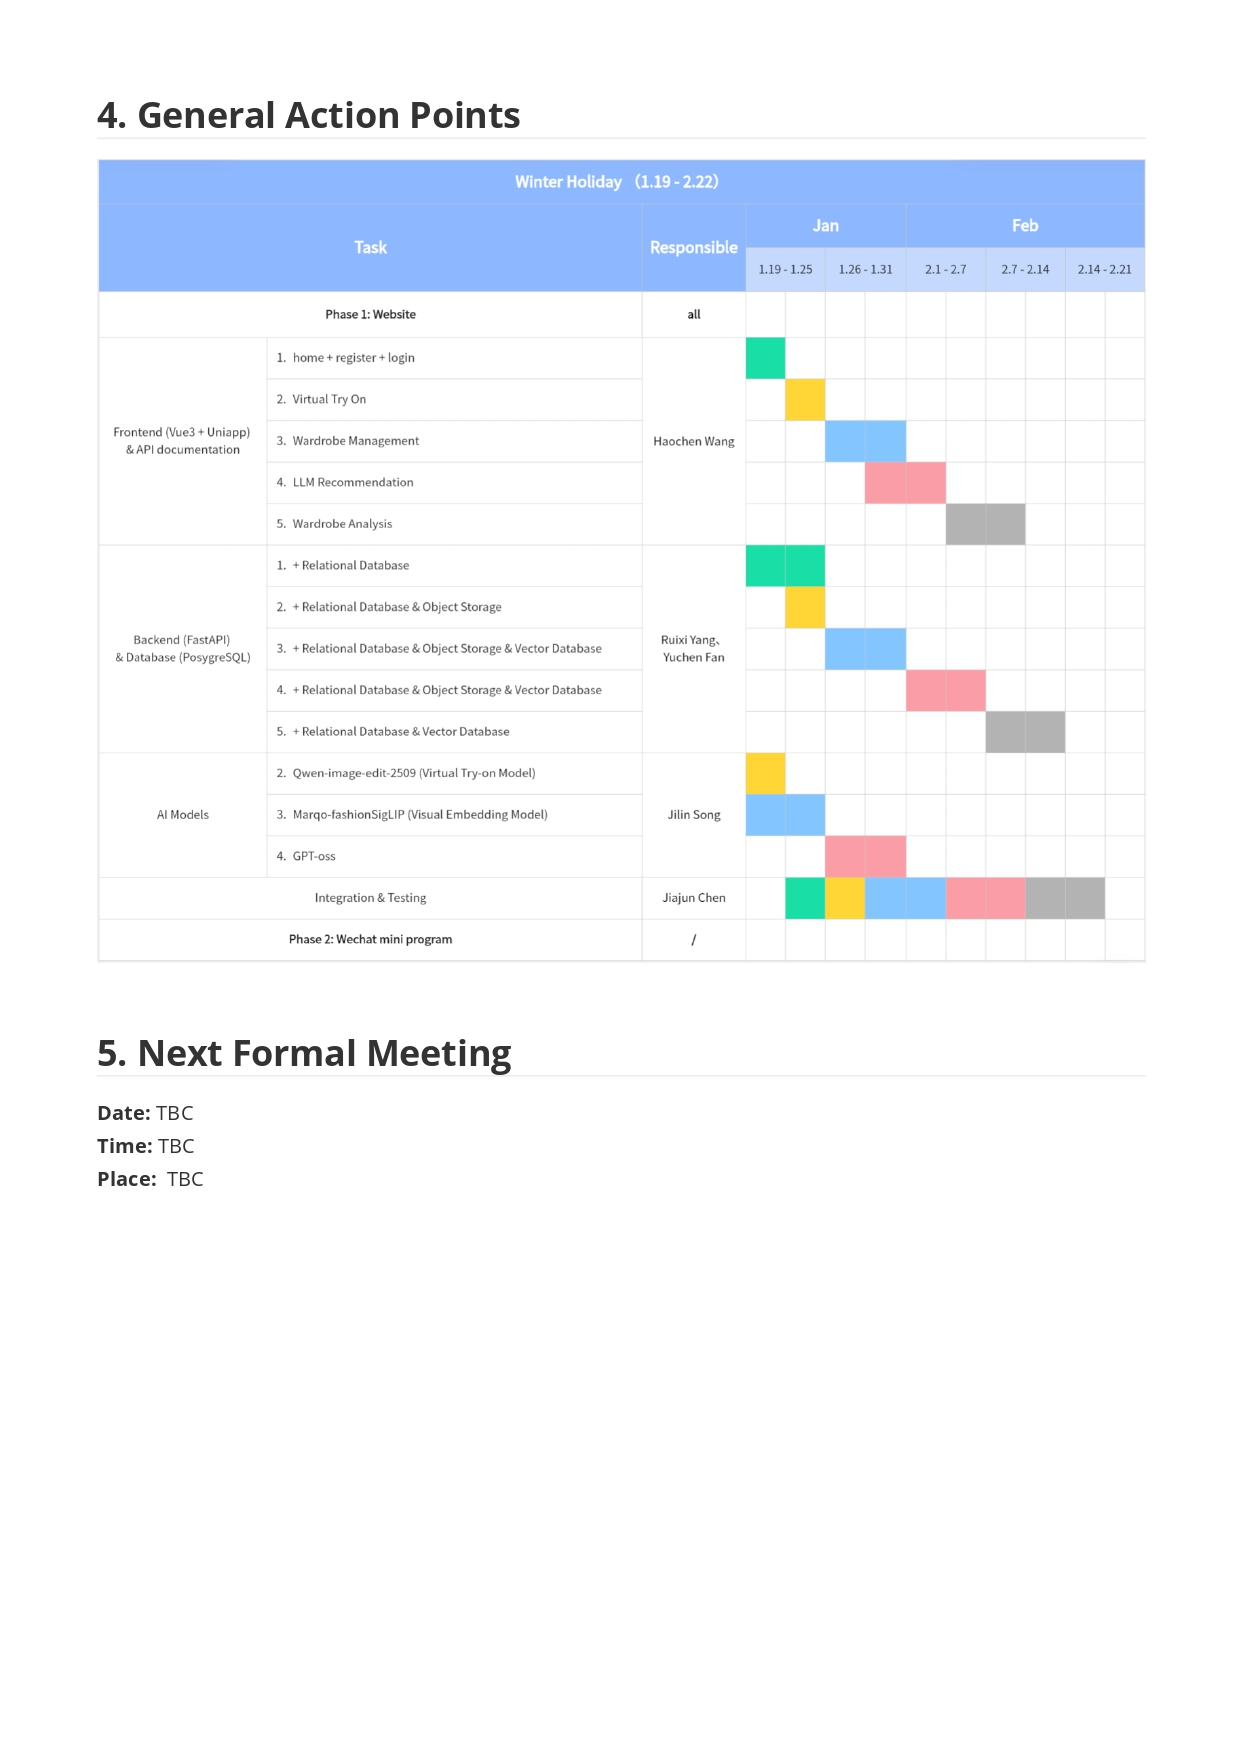
\includegraphics[width=1.0\textwidth]{images/appendix/8th_Formal_Meeting_Minutes_2026-02-02_page-0003.jpg}
\end{figure}


\section{9th Formal Meeting Minutes (2026-02-27)}
\begin{figure}[H]
    \centering
    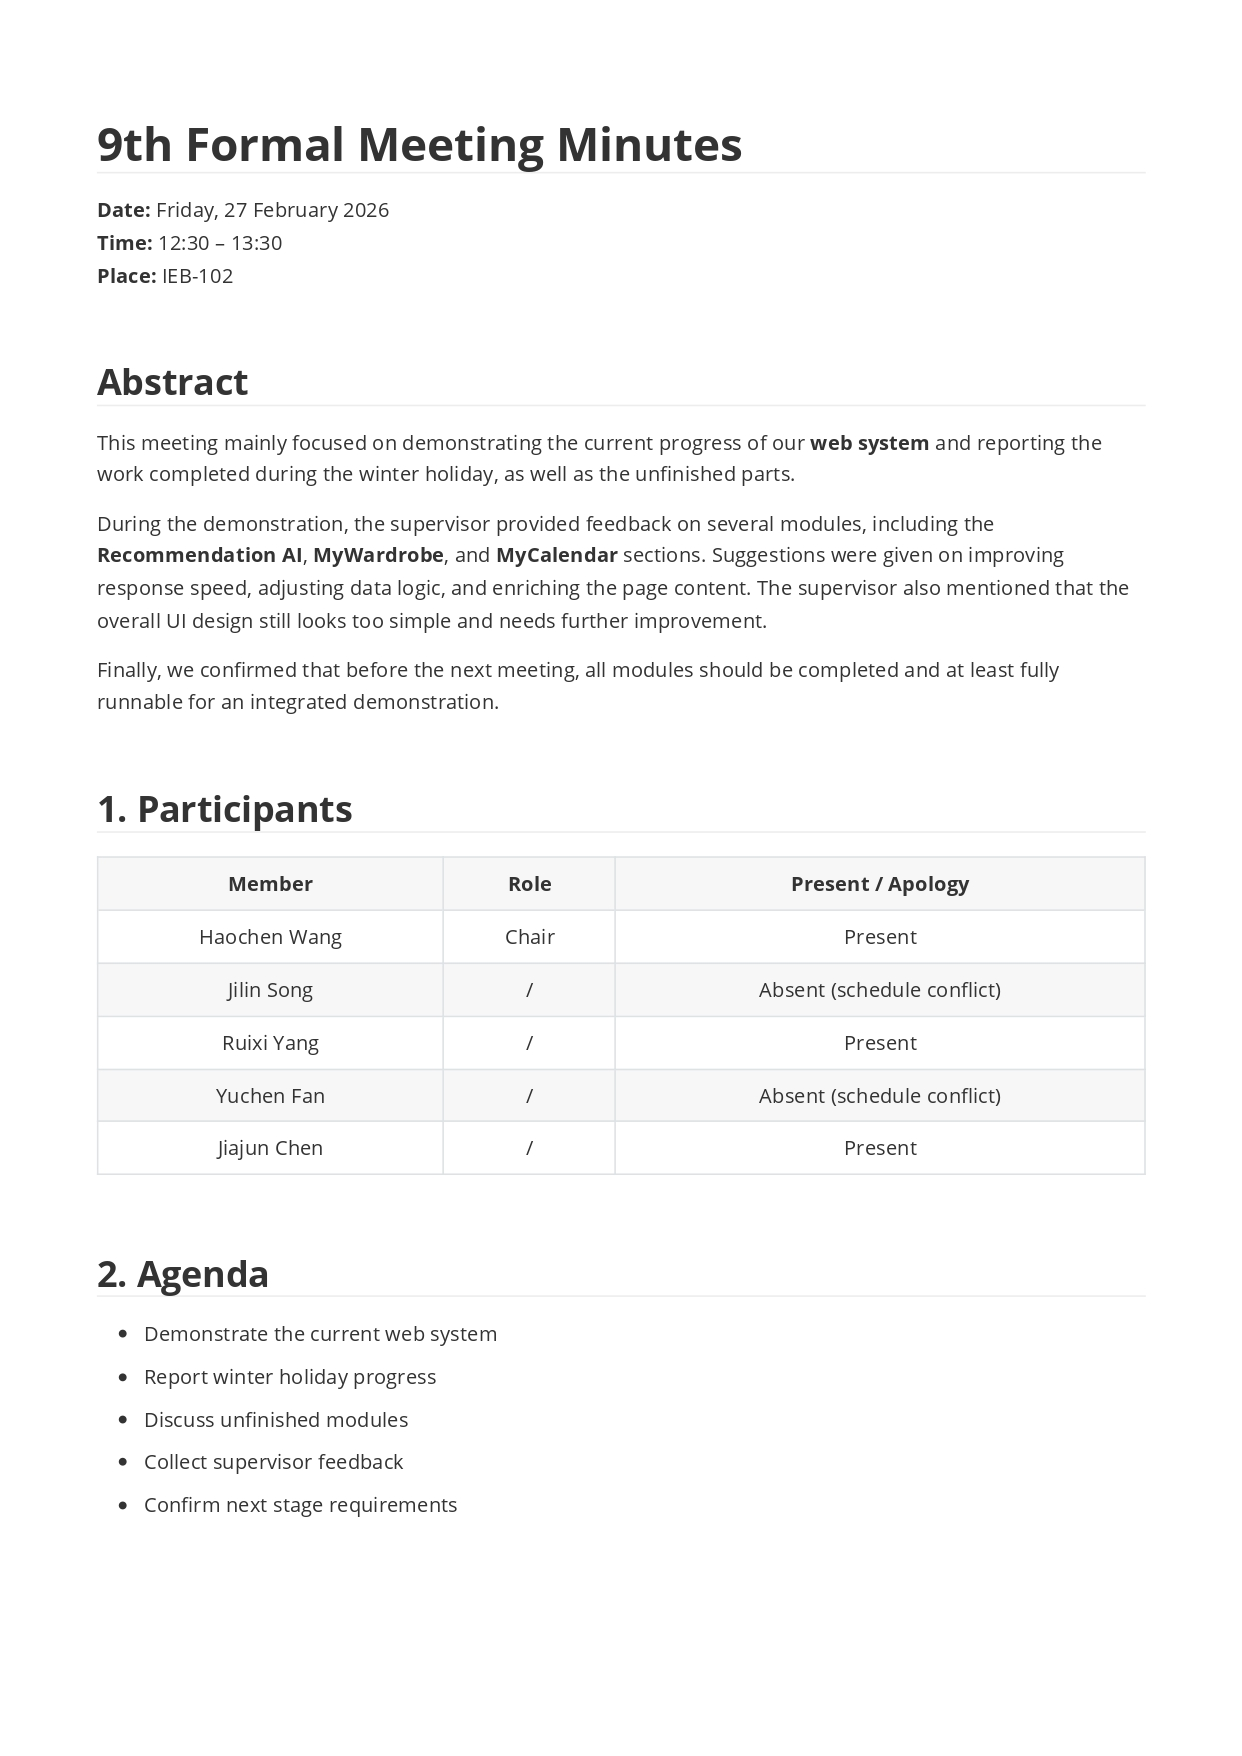
\includegraphics[width=1.0\textwidth]{images/appendix/9th_Formal_Meeting_Minutes_2026-02-27_page-0001.jpg}
\end{figure}
\begin{figure}[H]
    \centering
    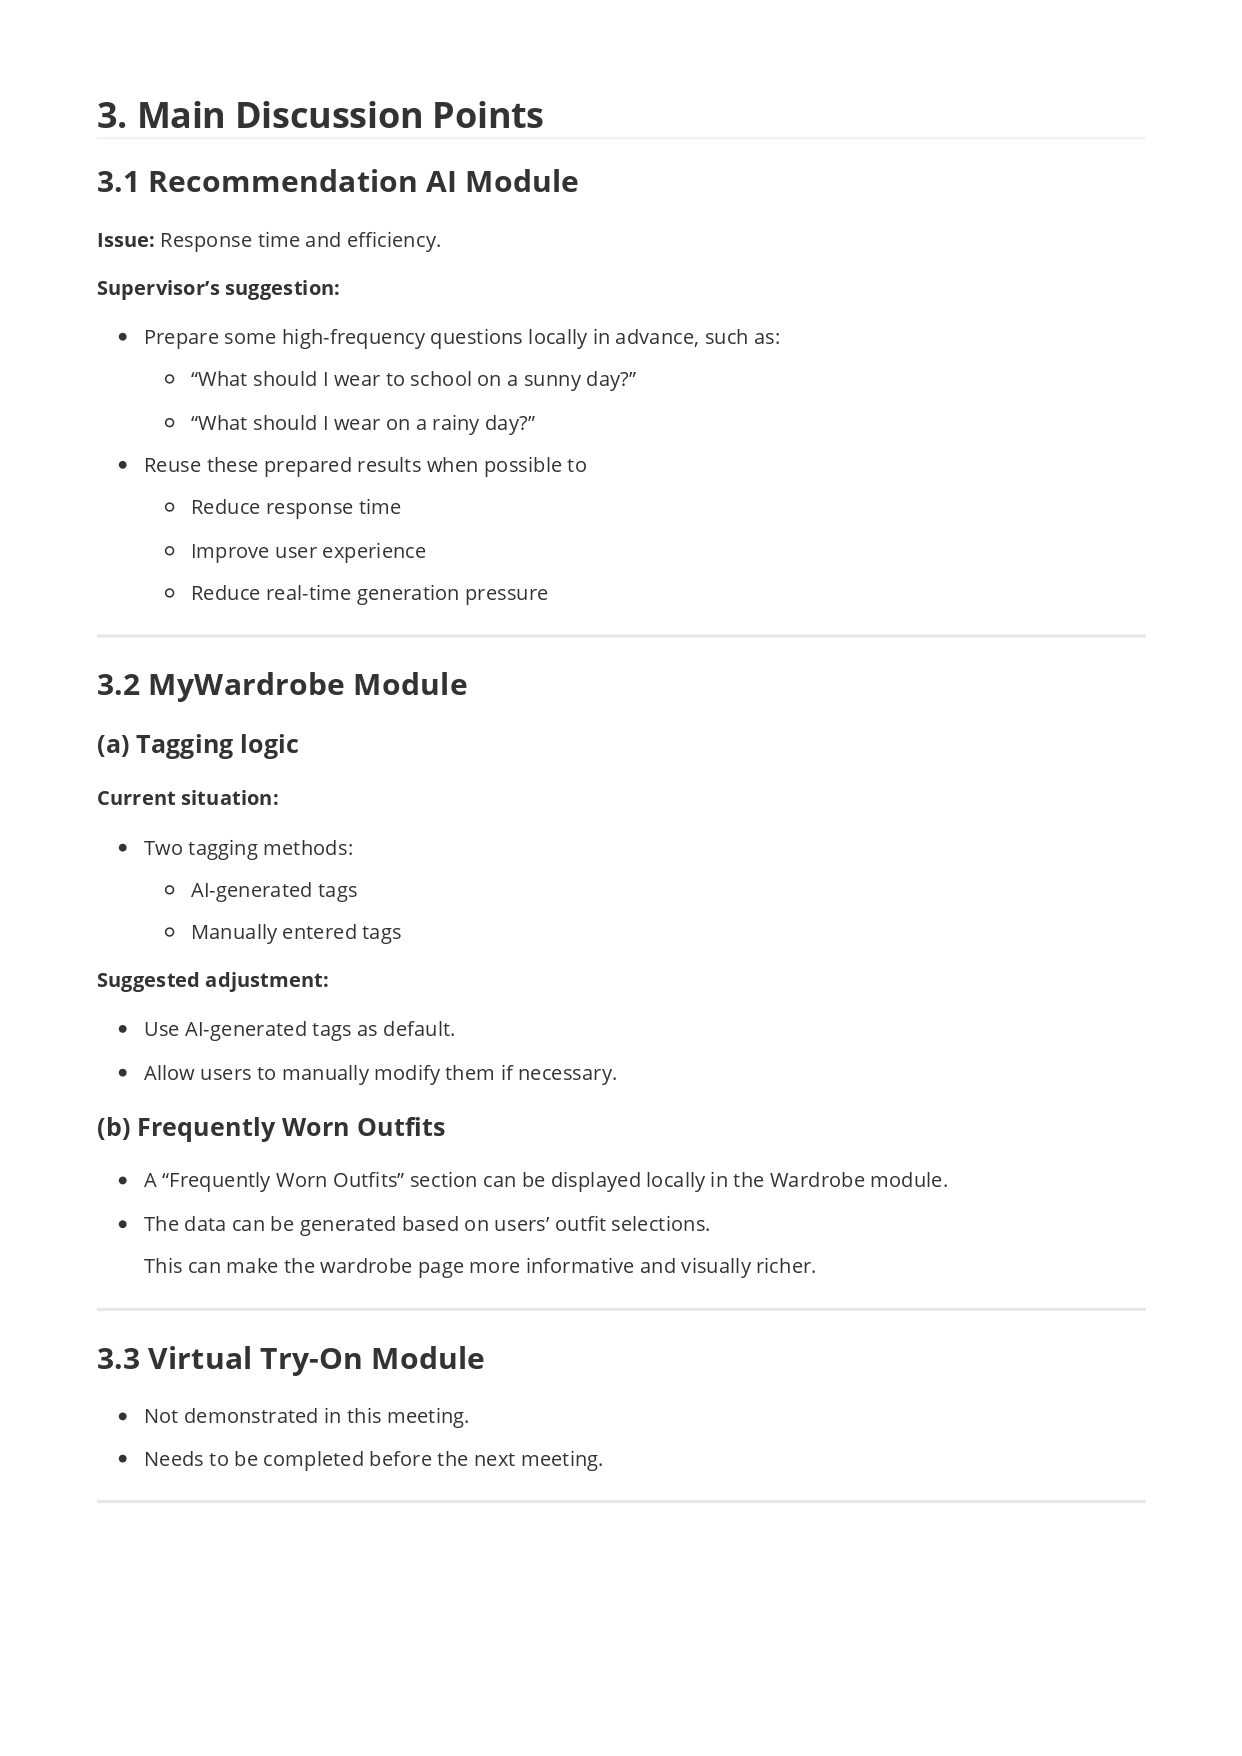
\includegraphics[width=1.0\textwidth]{images/appendix/9th_Formal_Meeting_Minutes_2026-02-27_page-0002.jpg}
\end{figure}
\begin{figure}[H]
    \centering
    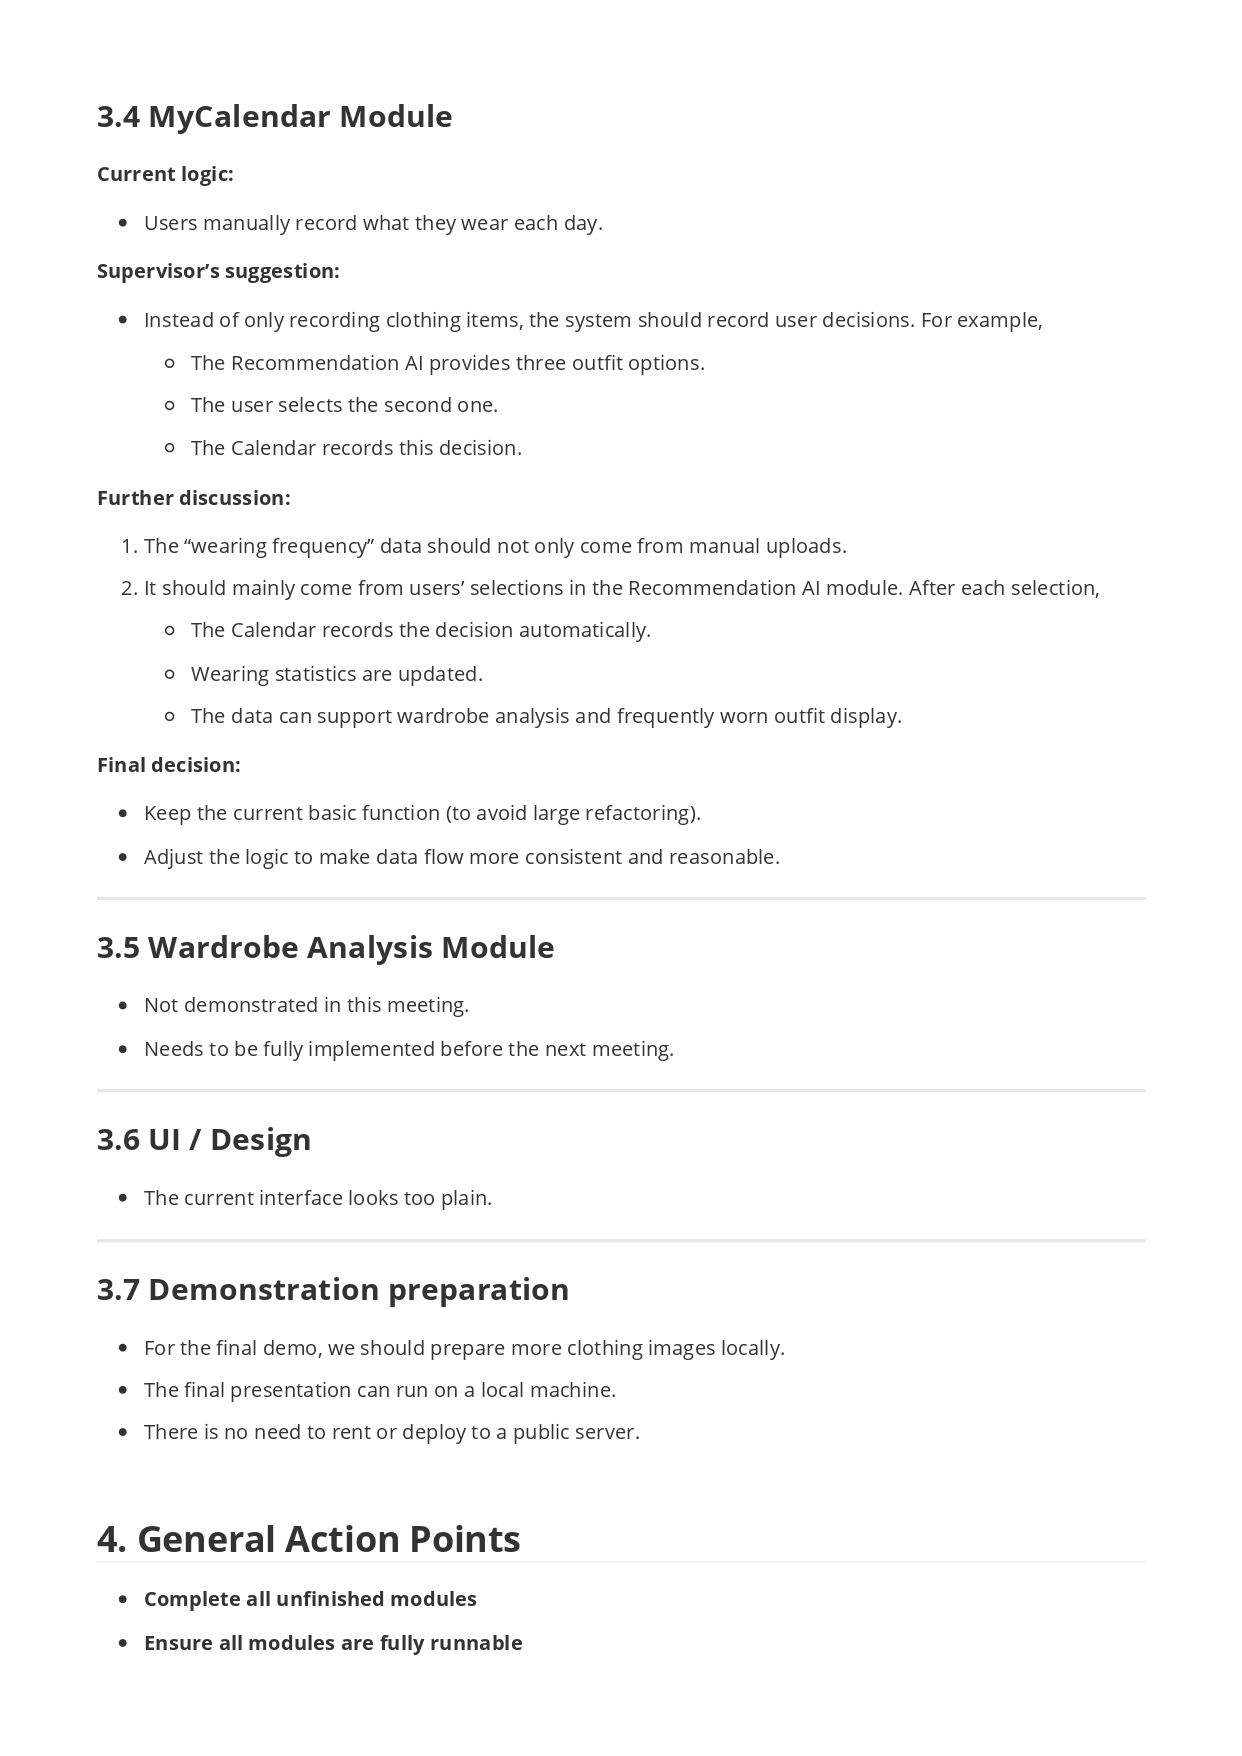
\includegraphics[width=1.0\textwidth]{images/appendix/9th_Formal_Meeting_Minutes_2026-02-27_page-0003.jpg}
\end{figure}
\begin{figure}[H]
    \centering
    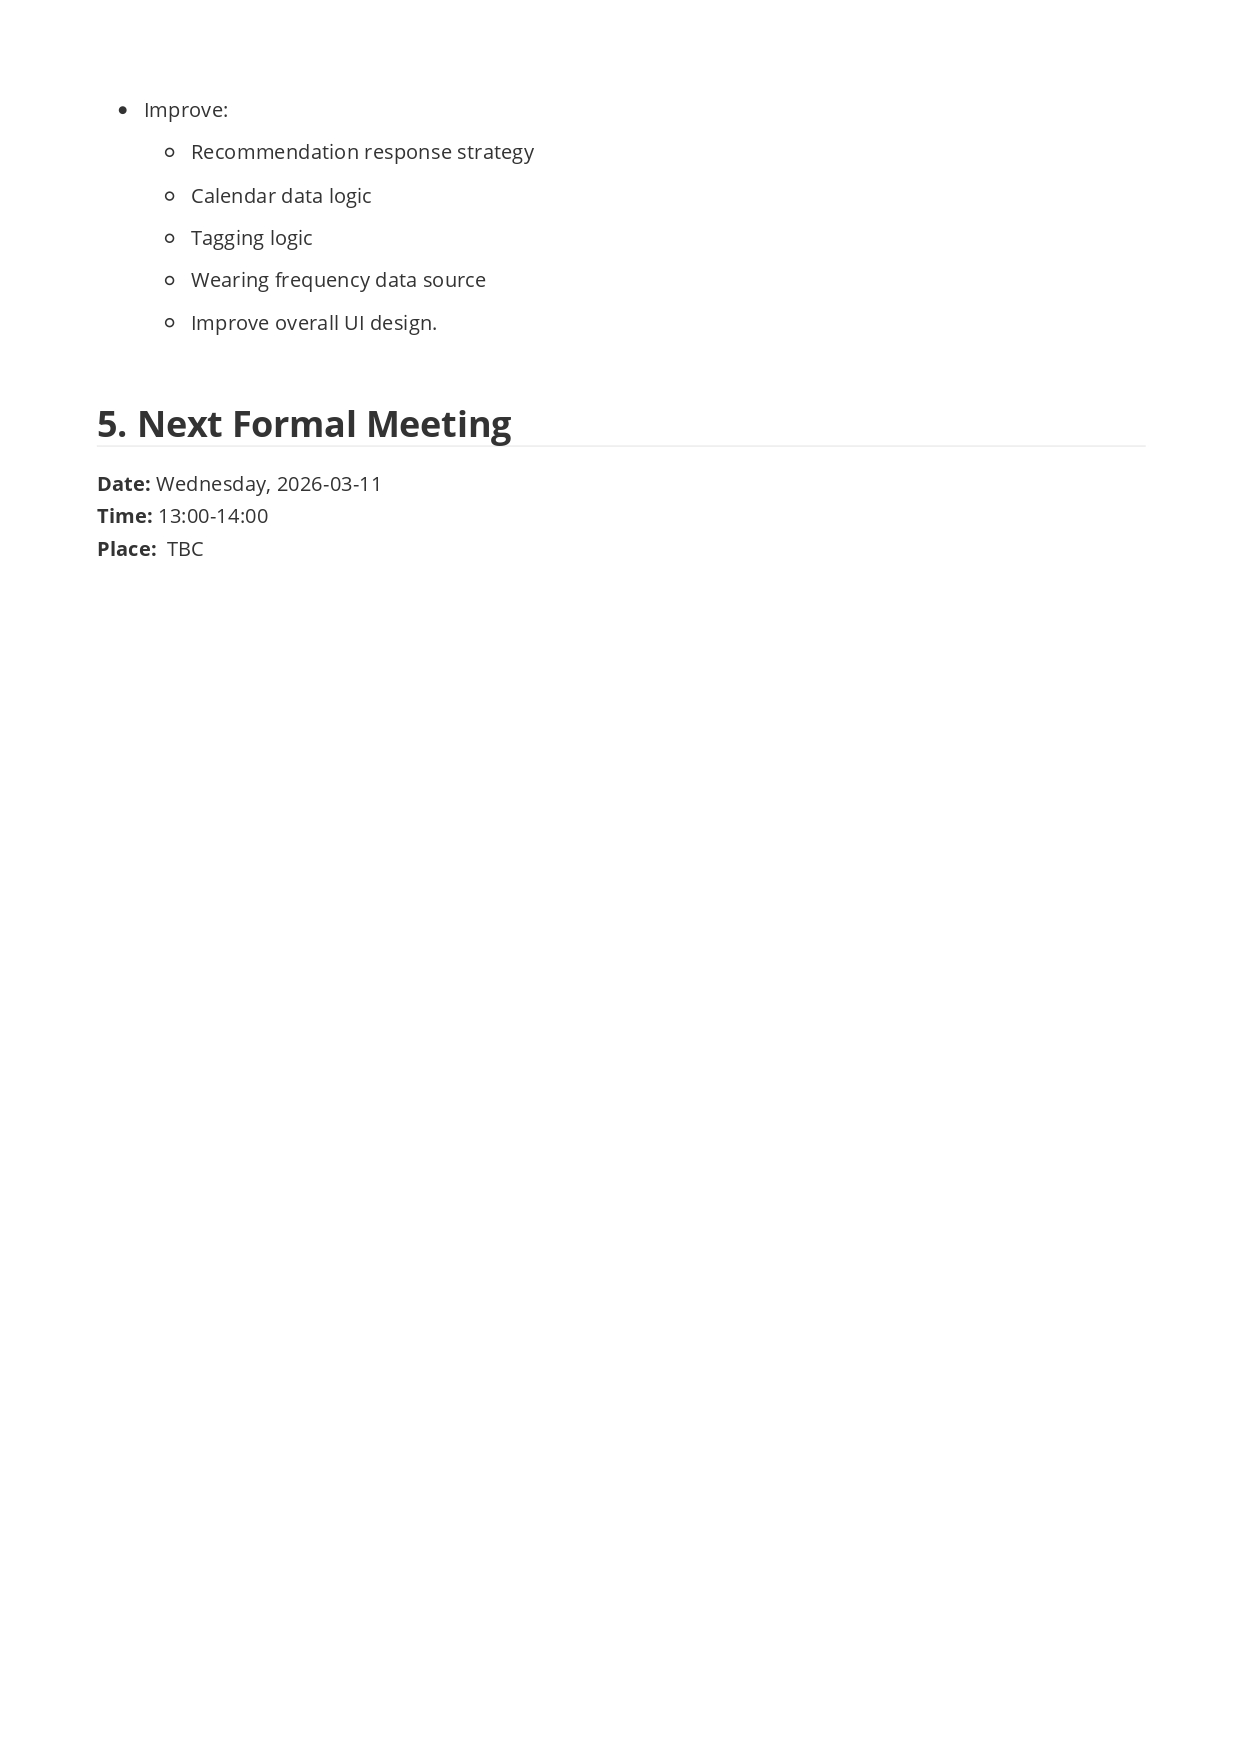
\includegraphics[width=1.0\textwidth]{images/appendix/9th_Formal_Meeting_Minutes_2026-02-27_page-0004.jpg}
\end{figure}


\section{9th Informal Meeting Minutes (2026-02-25)}
\begin{figure}[H]
    \centering
    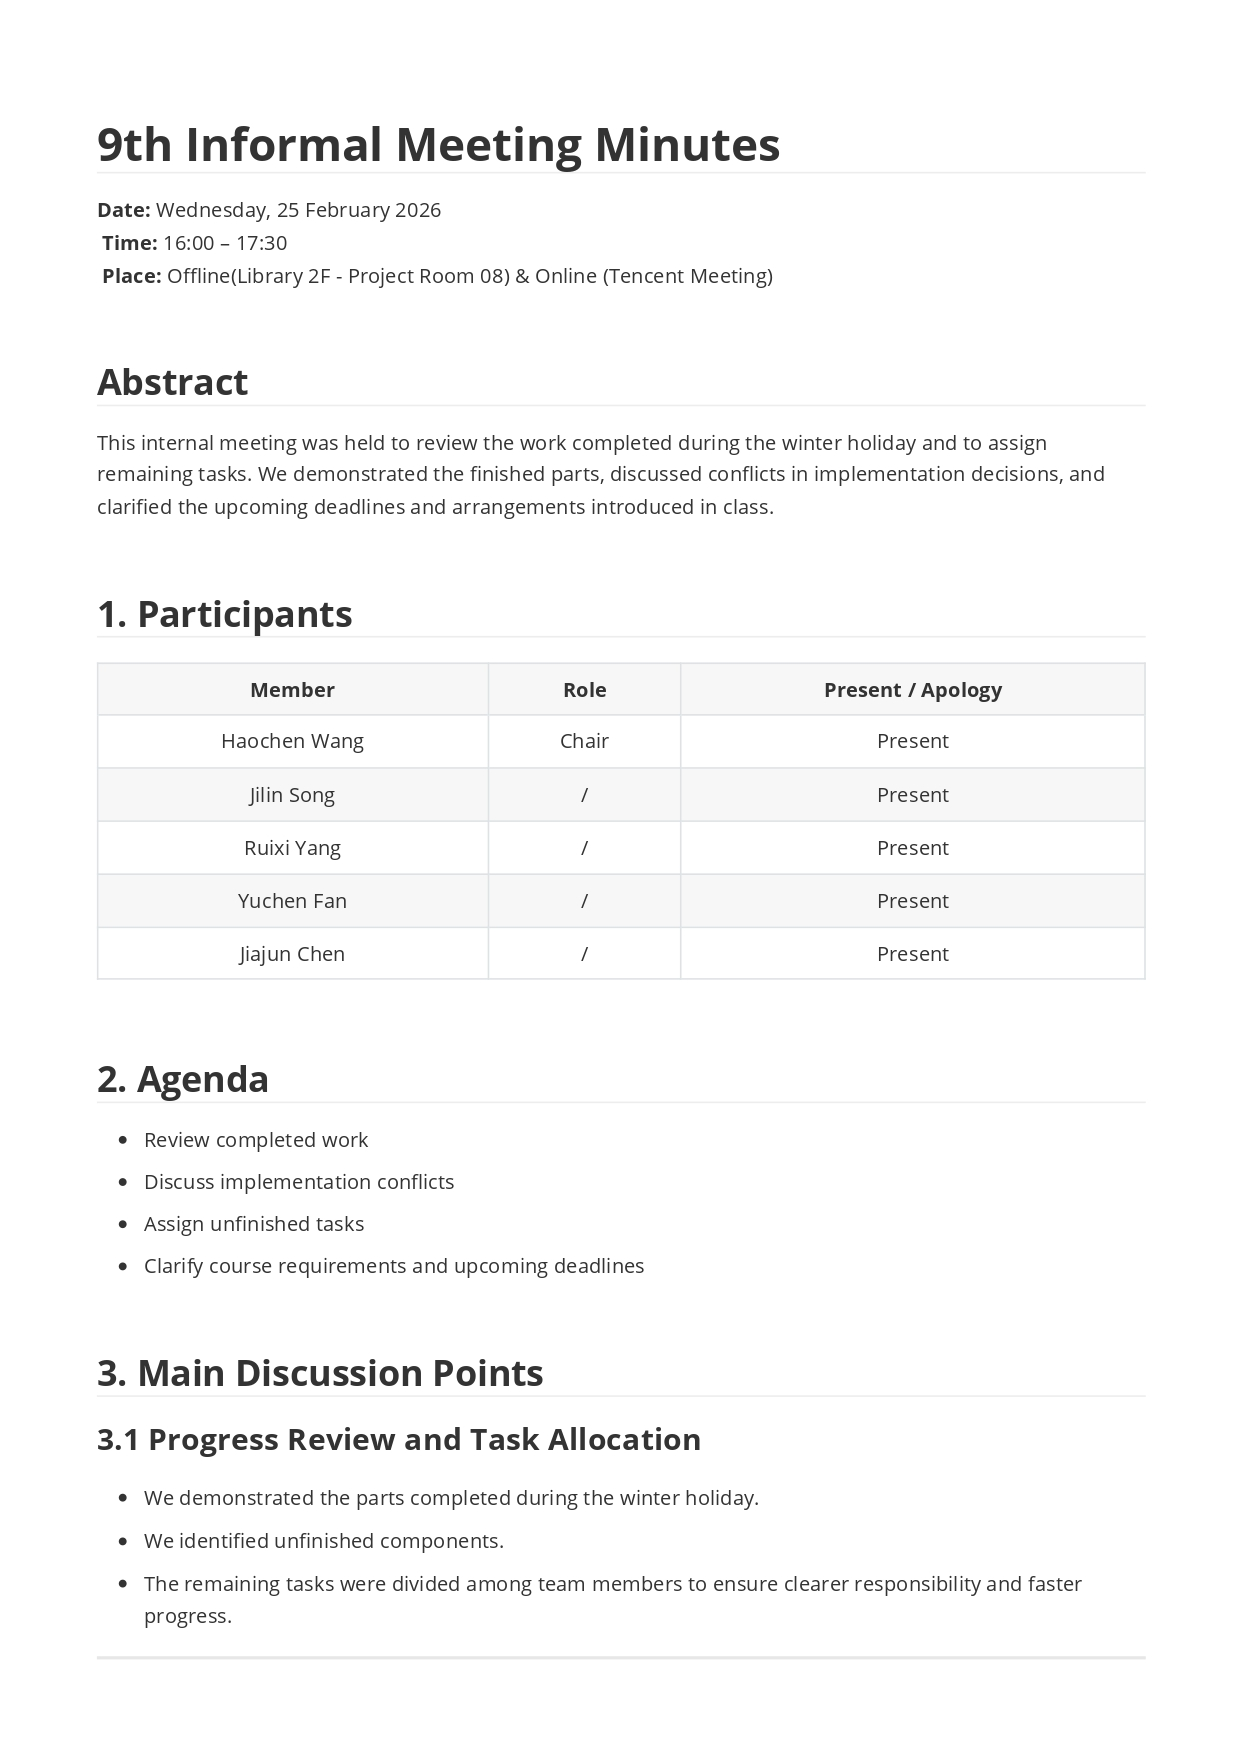
\includegraphics[width=1.0\textwidth]{images/appendix/9th_Informal_Meeting_Minutes_2026-02-25_page-0001.jpg}
\end{figure}
\begin{figure}[H]
    \centering
    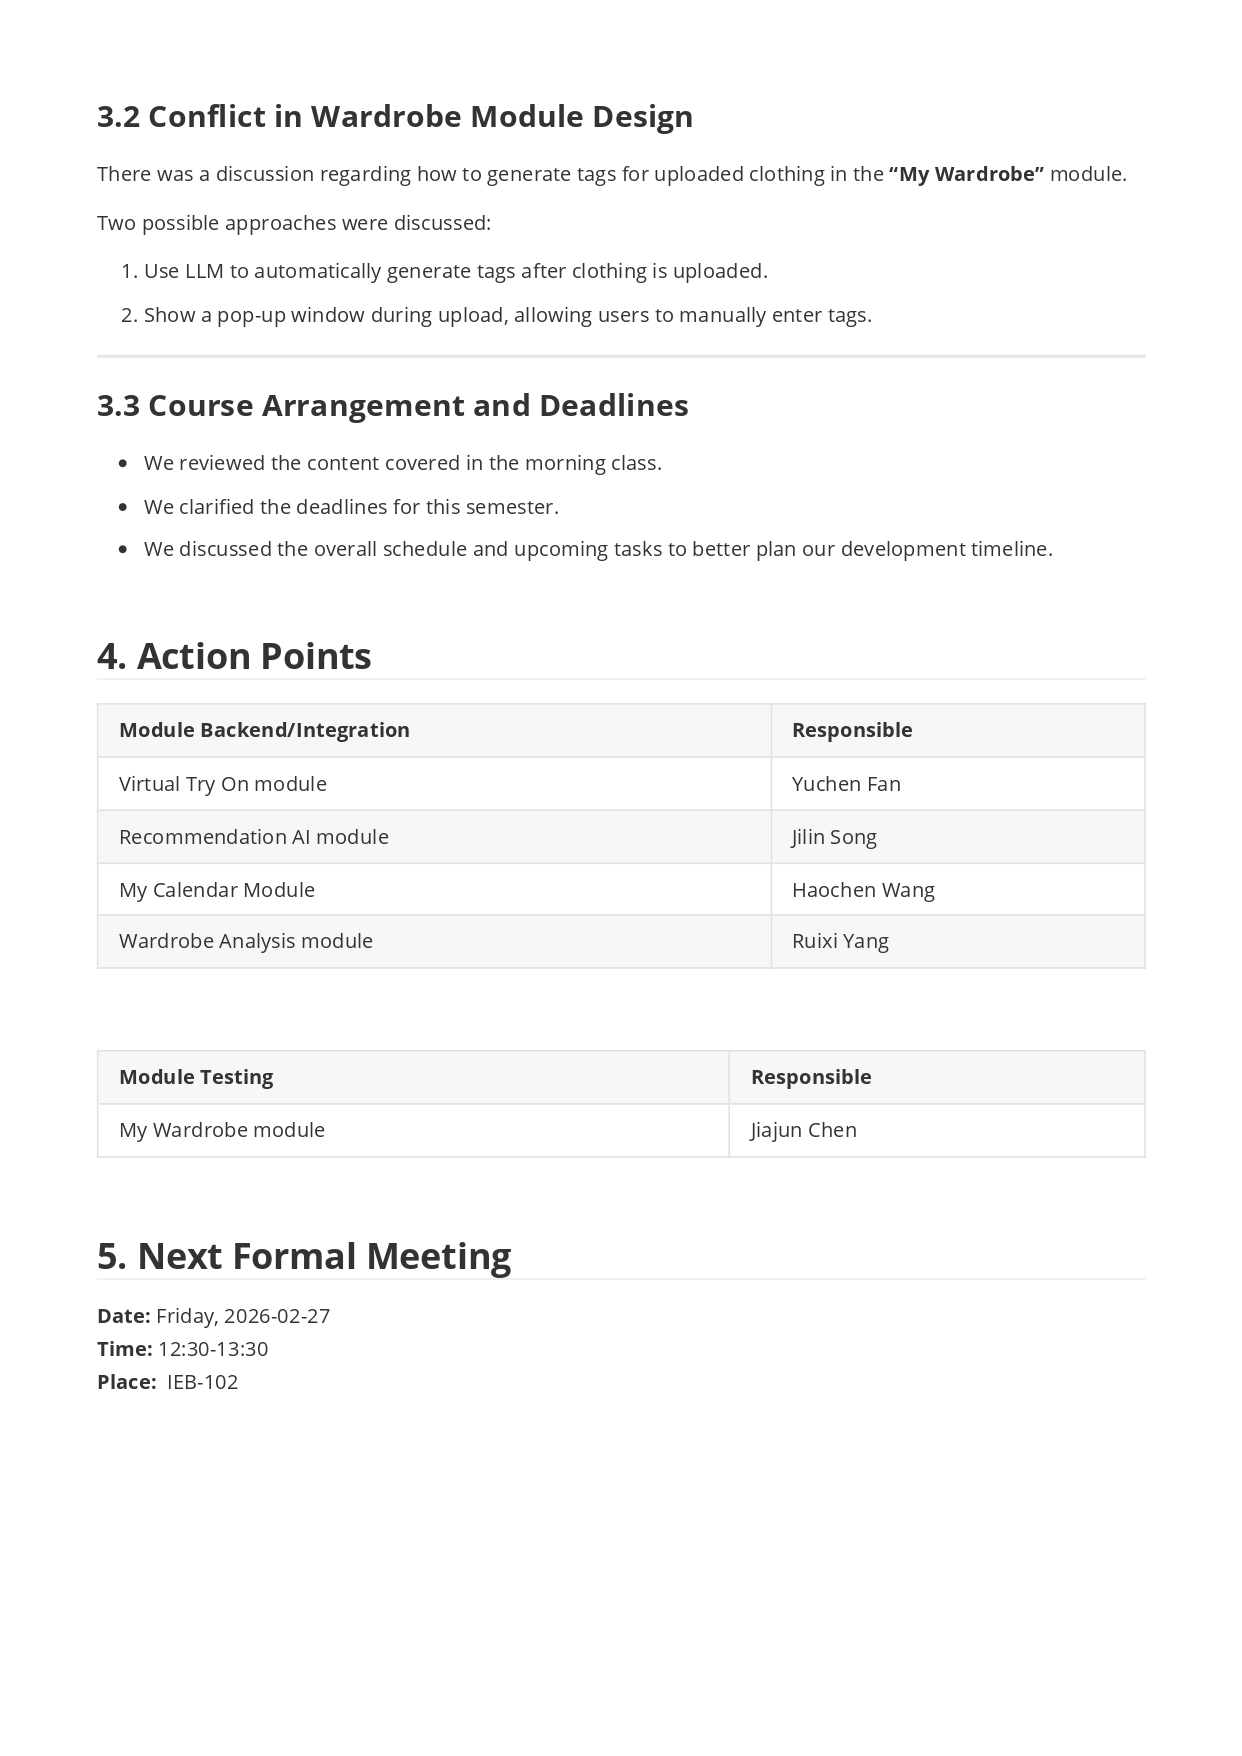
\includegraphics[width=1.0\textwidth]{images/appendix/9th_Informal_Meeting_Minutes_2026-02-25_page-0002.jpg}
\end{figure}


\section{10th Formal Meeting Minutes (2026-03-18)}
\begin{figure}[H]
    \centering
    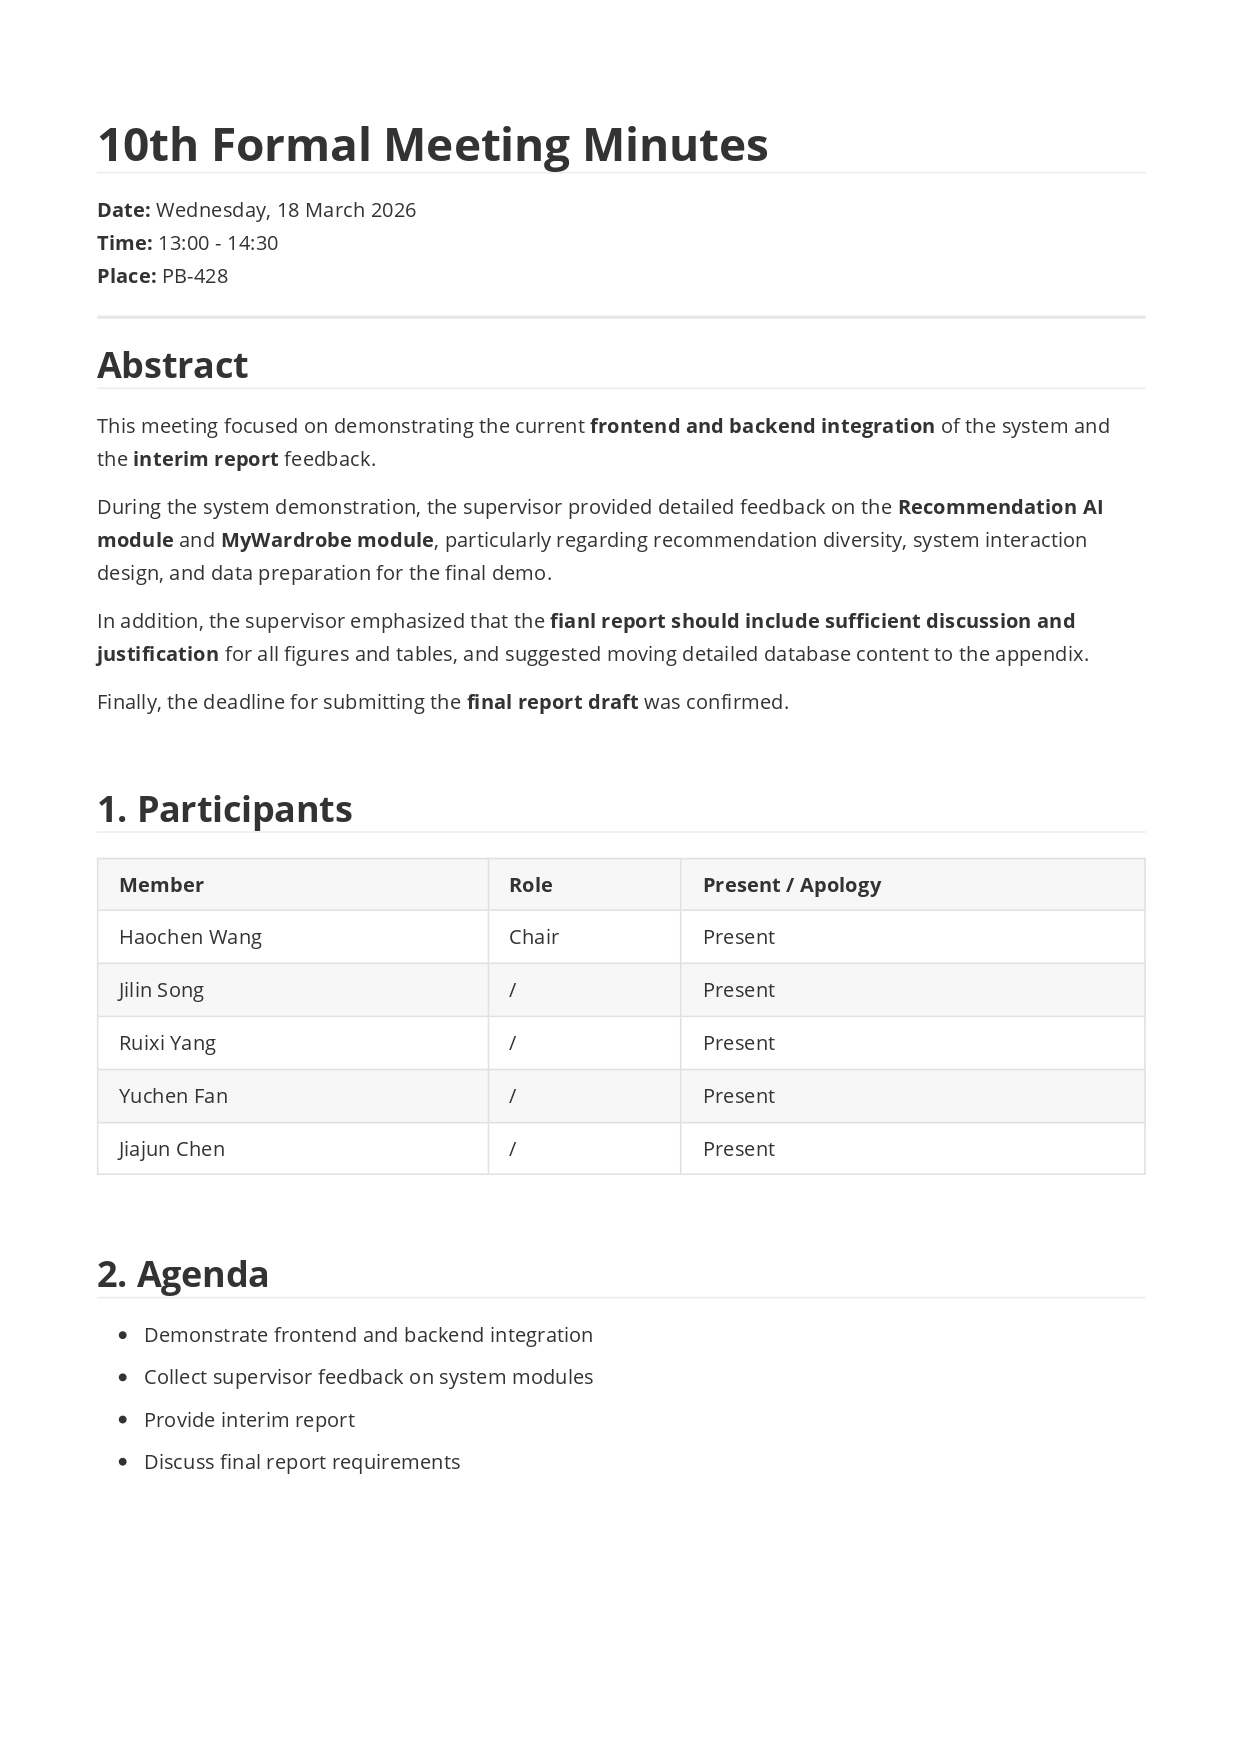
\includegraphics[width=1.0\textwidth]{images/appendix/10th_Formal_Meeting_Minutes_2026-03-18_page-0001.jpg}
\end{figure}
\begin{figure}[H]
    \centering
    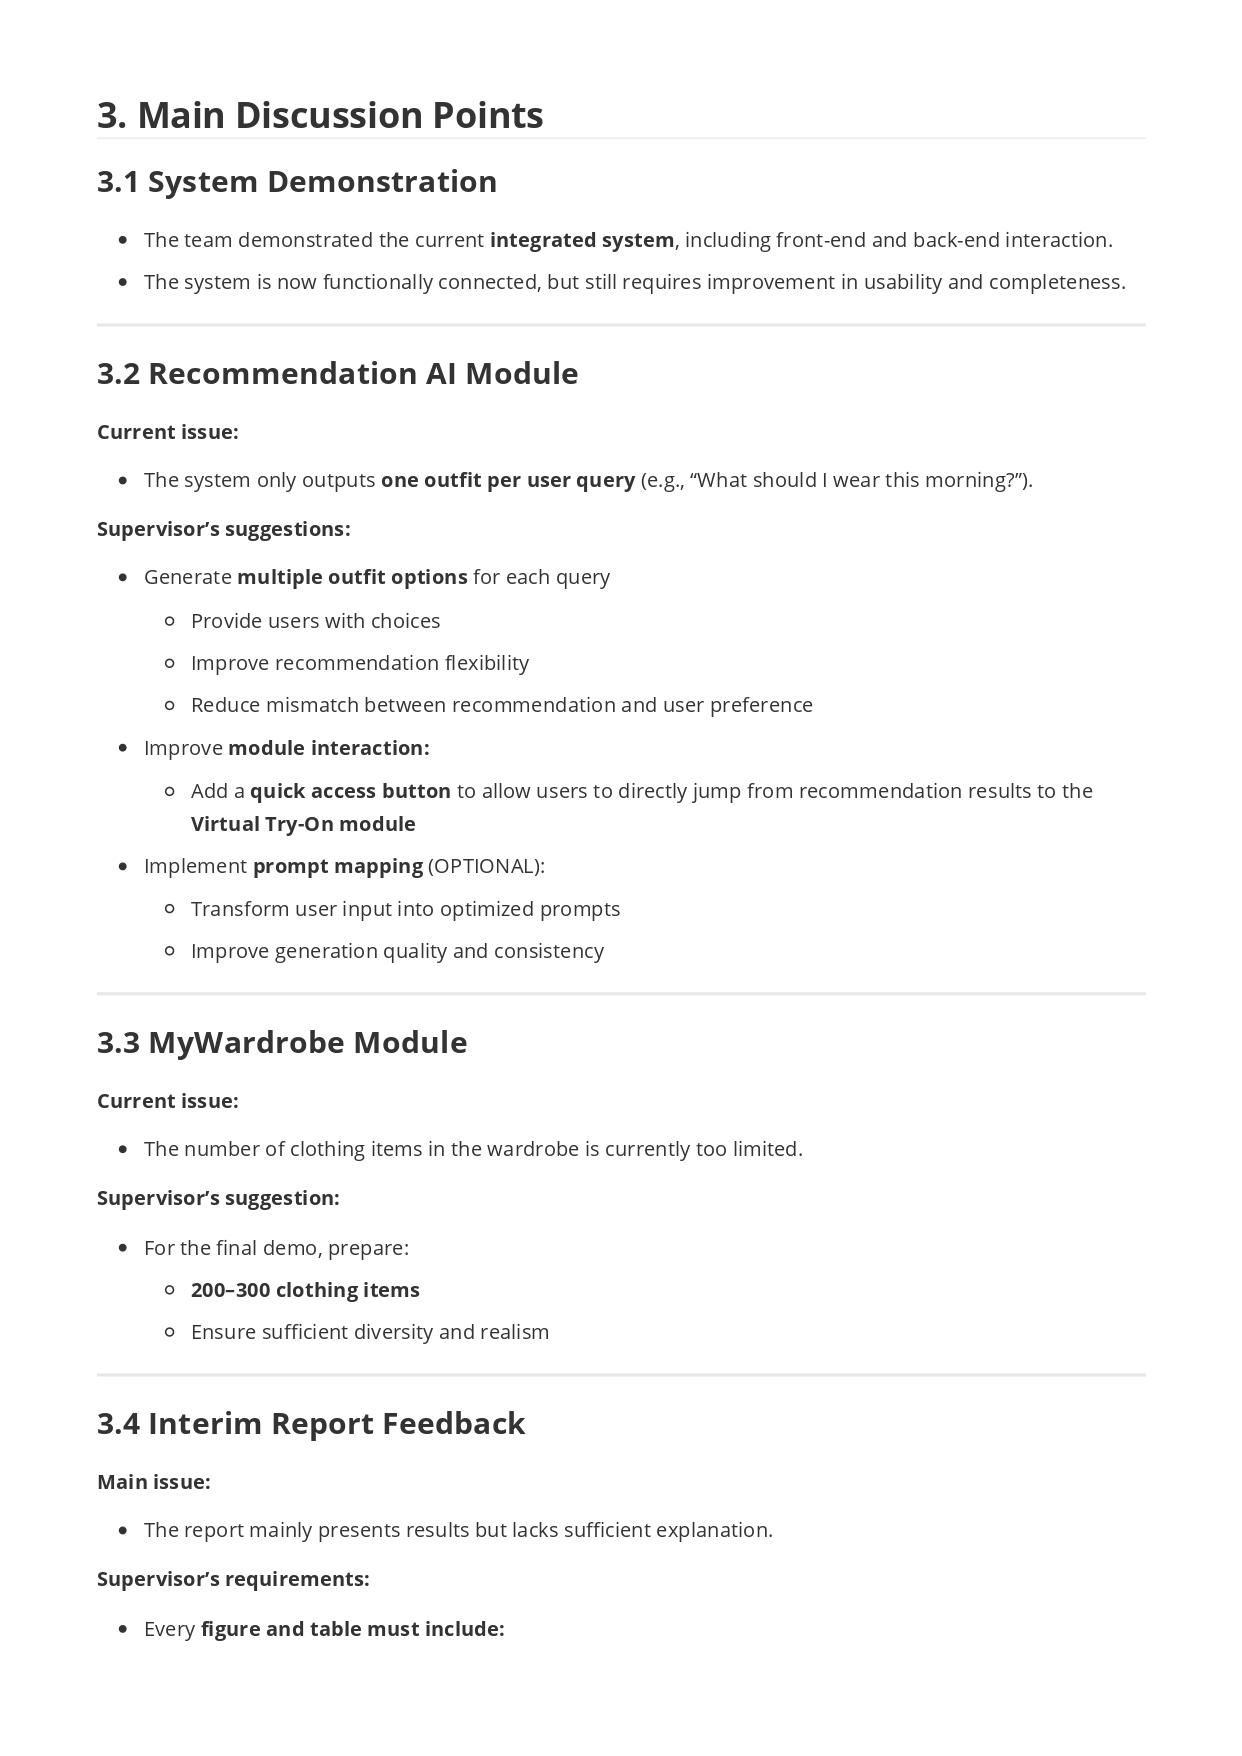
\includegraphics[width=1.0\textwidth]{images/appendix/10th_Formal_Meeting_Minutes_2026-03-18_page-0002.jpg}
\end{figure}
\begin{figure}[H]
    \centering
    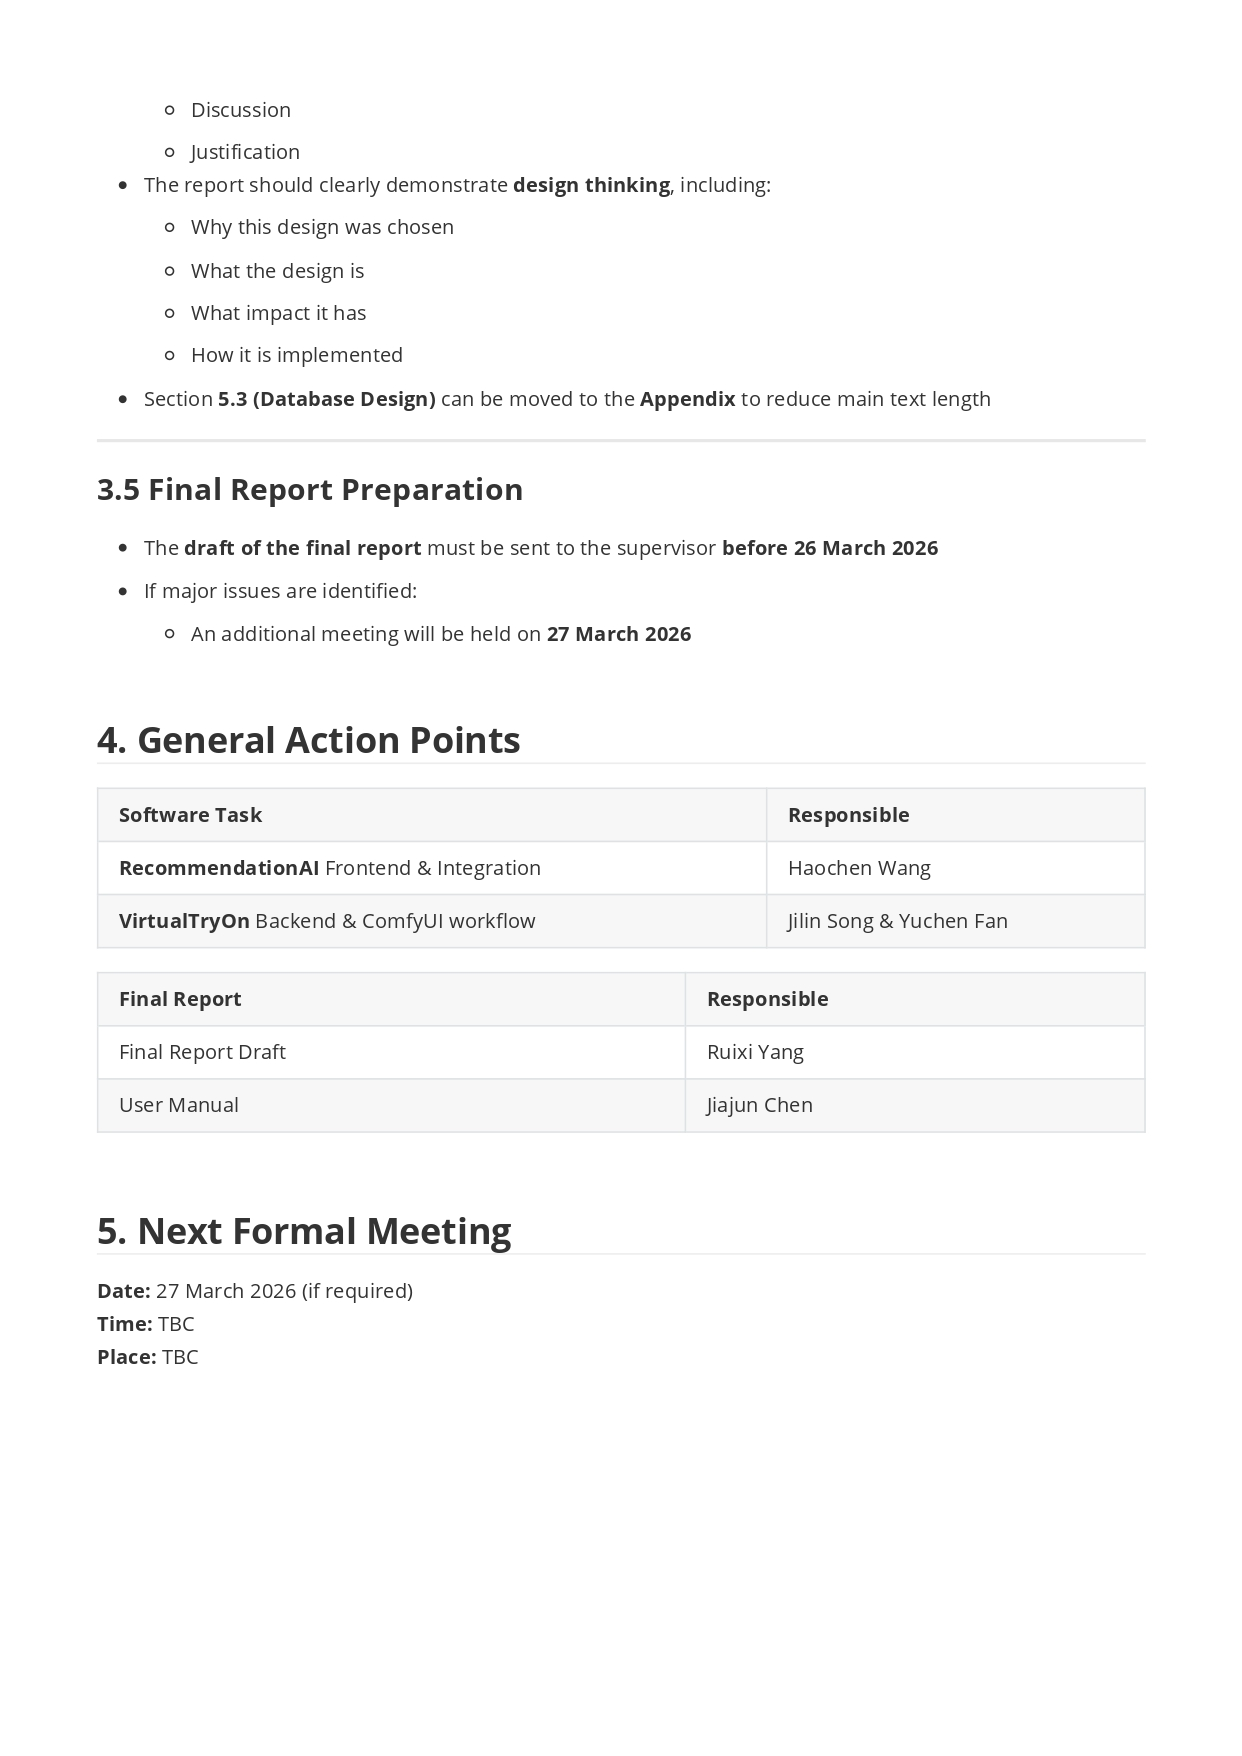
\includegraphics[width=1.0\textwidth]{images/appendix/10th_Formal_Meeting_Minutes_2026-03-18_page-0003.jpg}
\end{figure}



\section{10th Informal Meeting Minutes (2026-03-14)}
\begin{figure}[H]
    \centering
    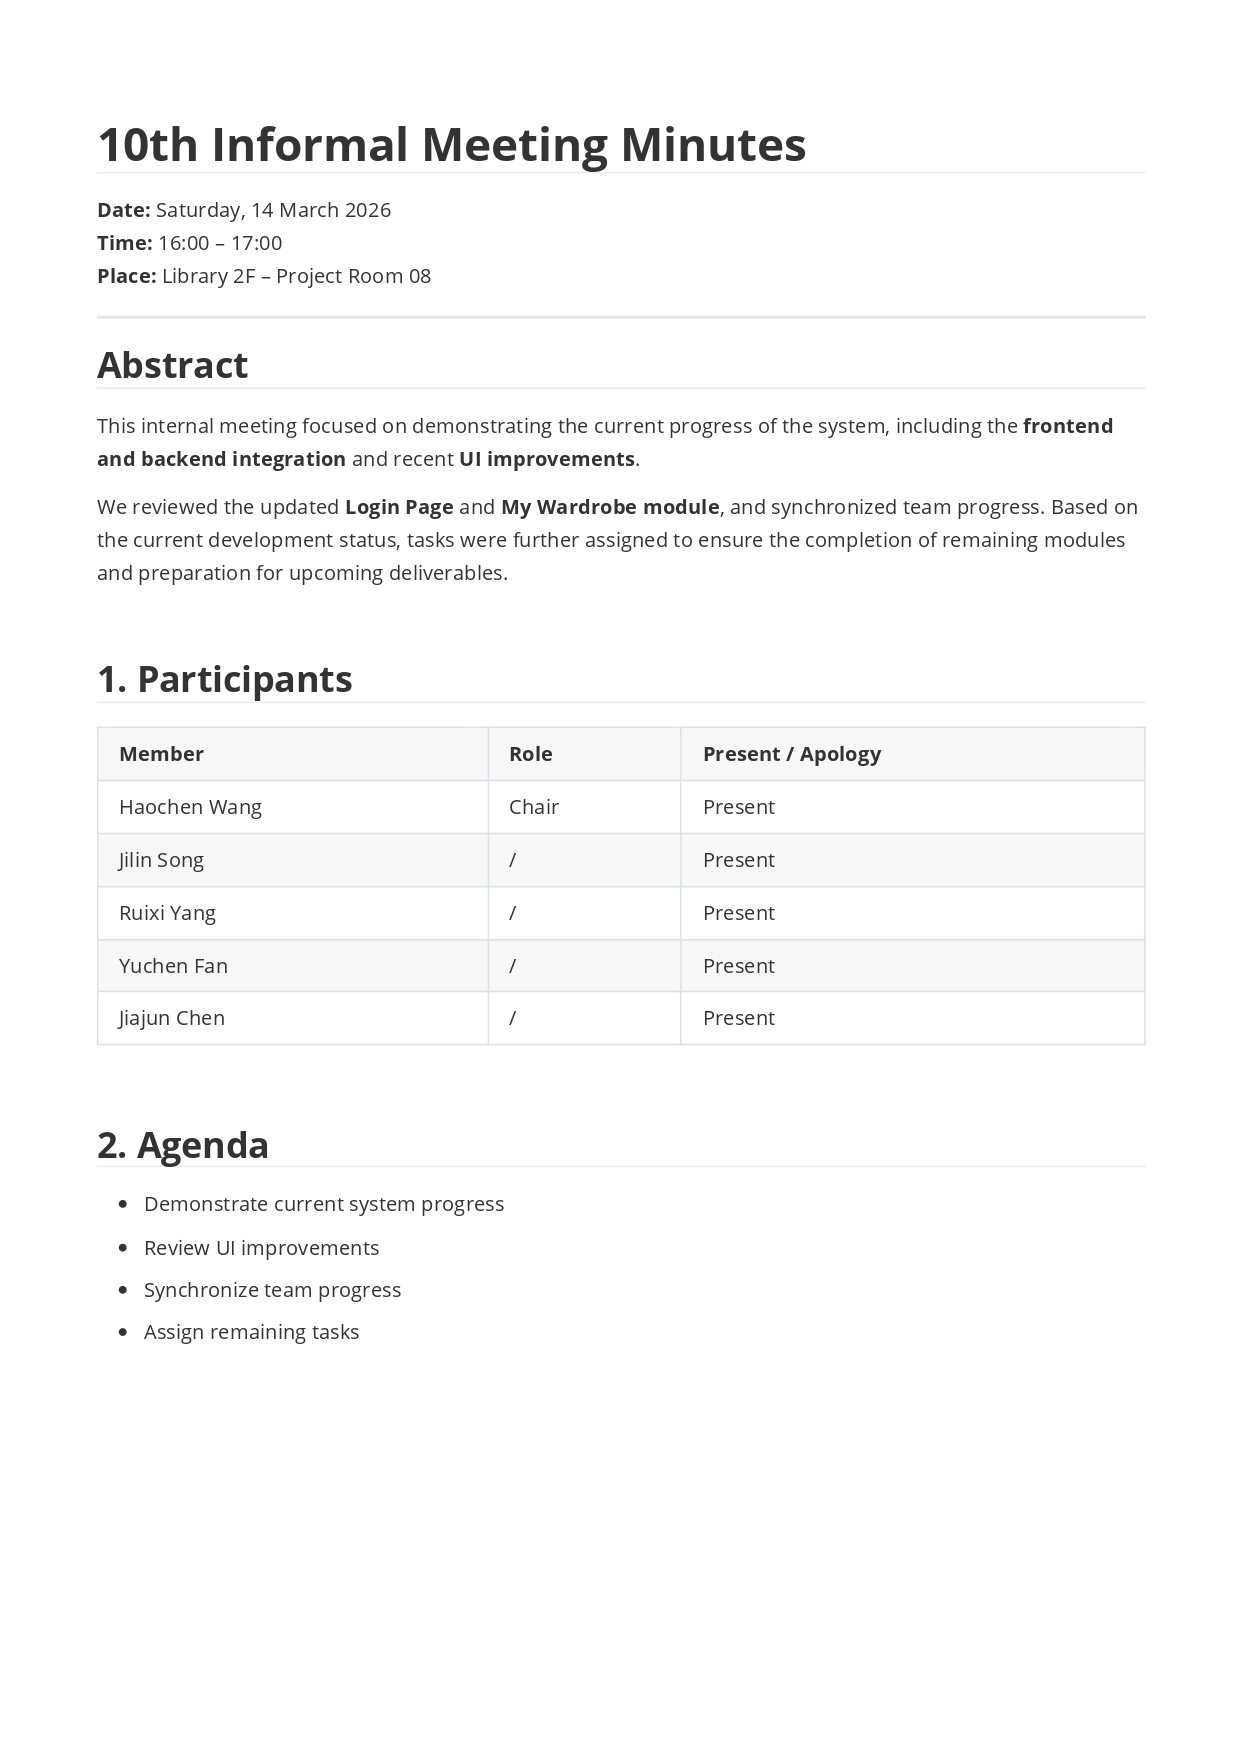
\includegraphics[width=1.0\textwidth]{images/appendix/10th_Informal_Meeting_Minutes_2026-03-14_page-0001.jpg}
\end{figure}
\begin{figure}[H]
    \centering
    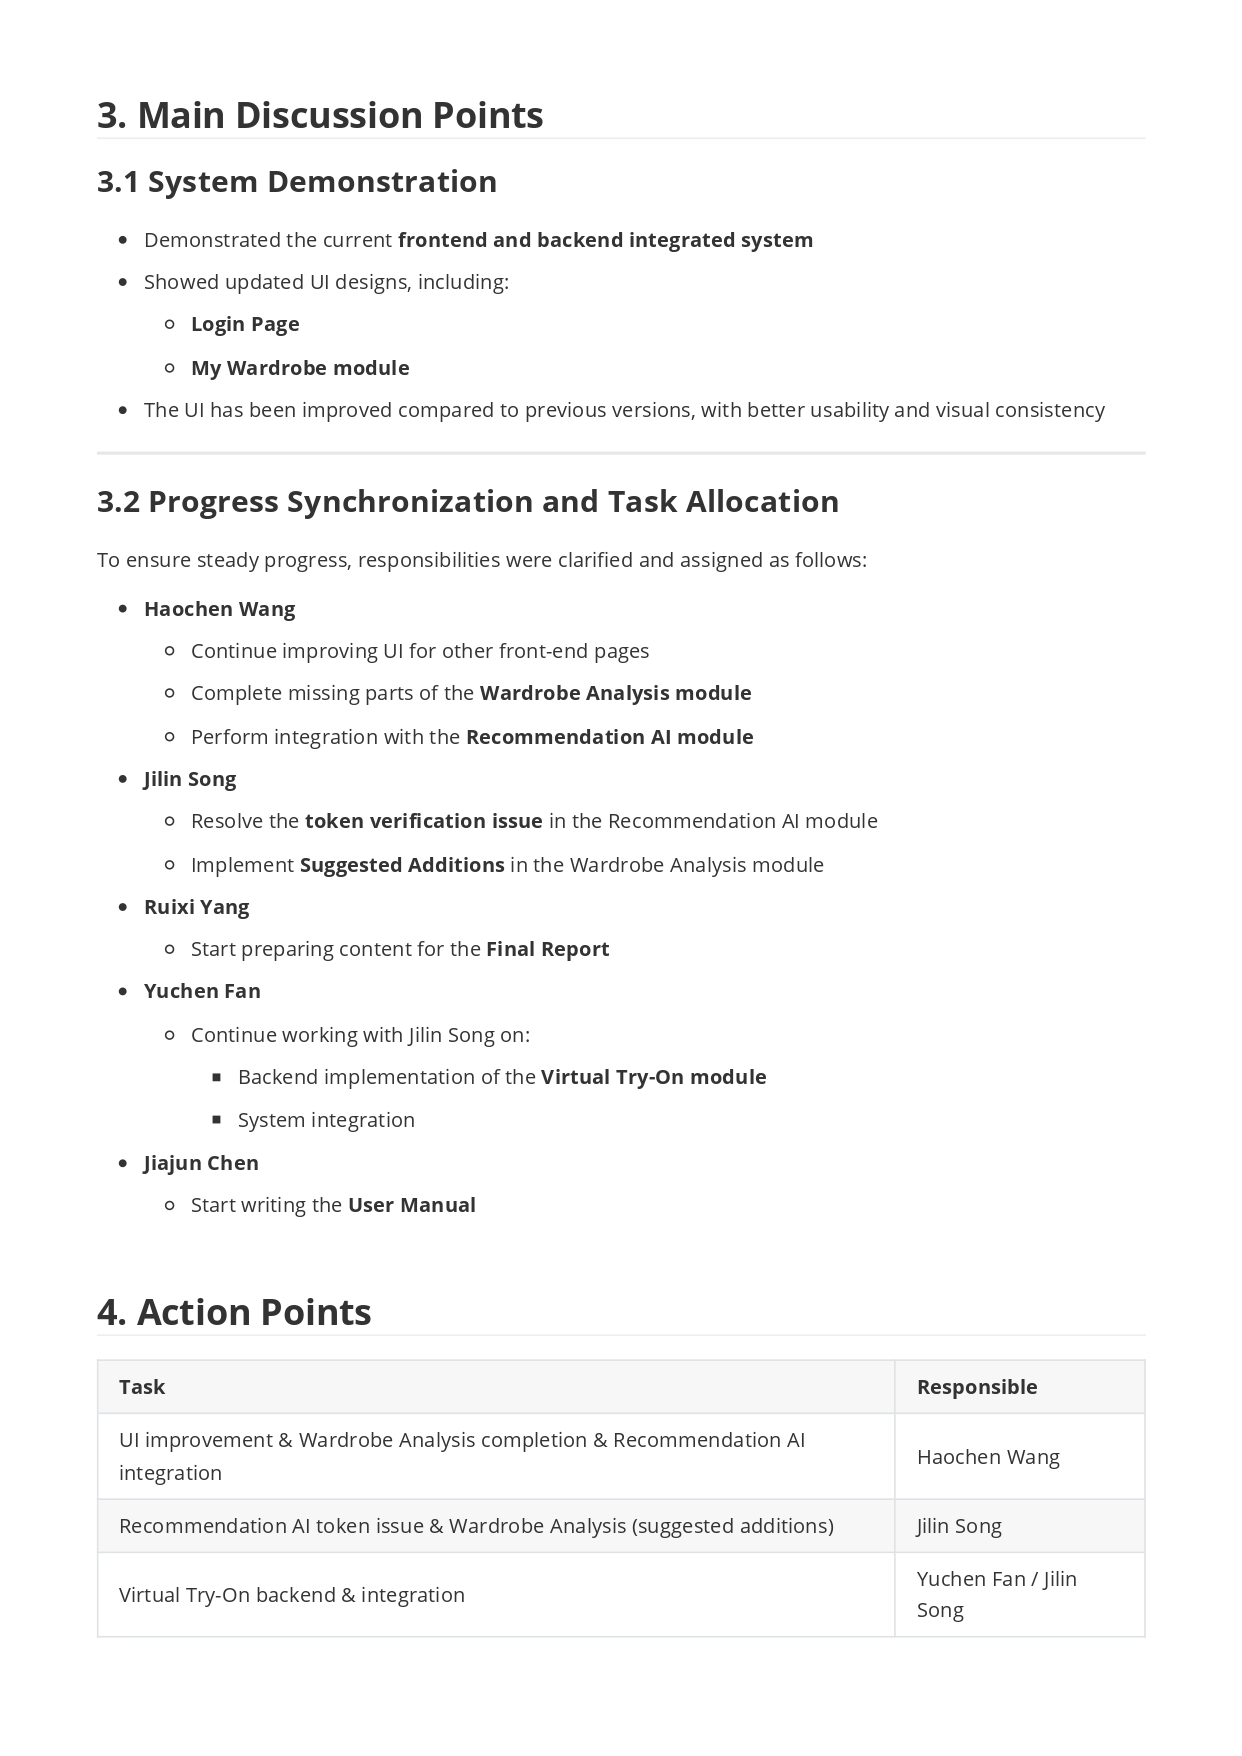
\includegraphics[width=1.0\textwidth]{images/appendix/10th_Informal_Meeting_Minutes_2026-03-14_page-0002.jpg}
\end{figure}
\begin{figure}[H]
    \centering
    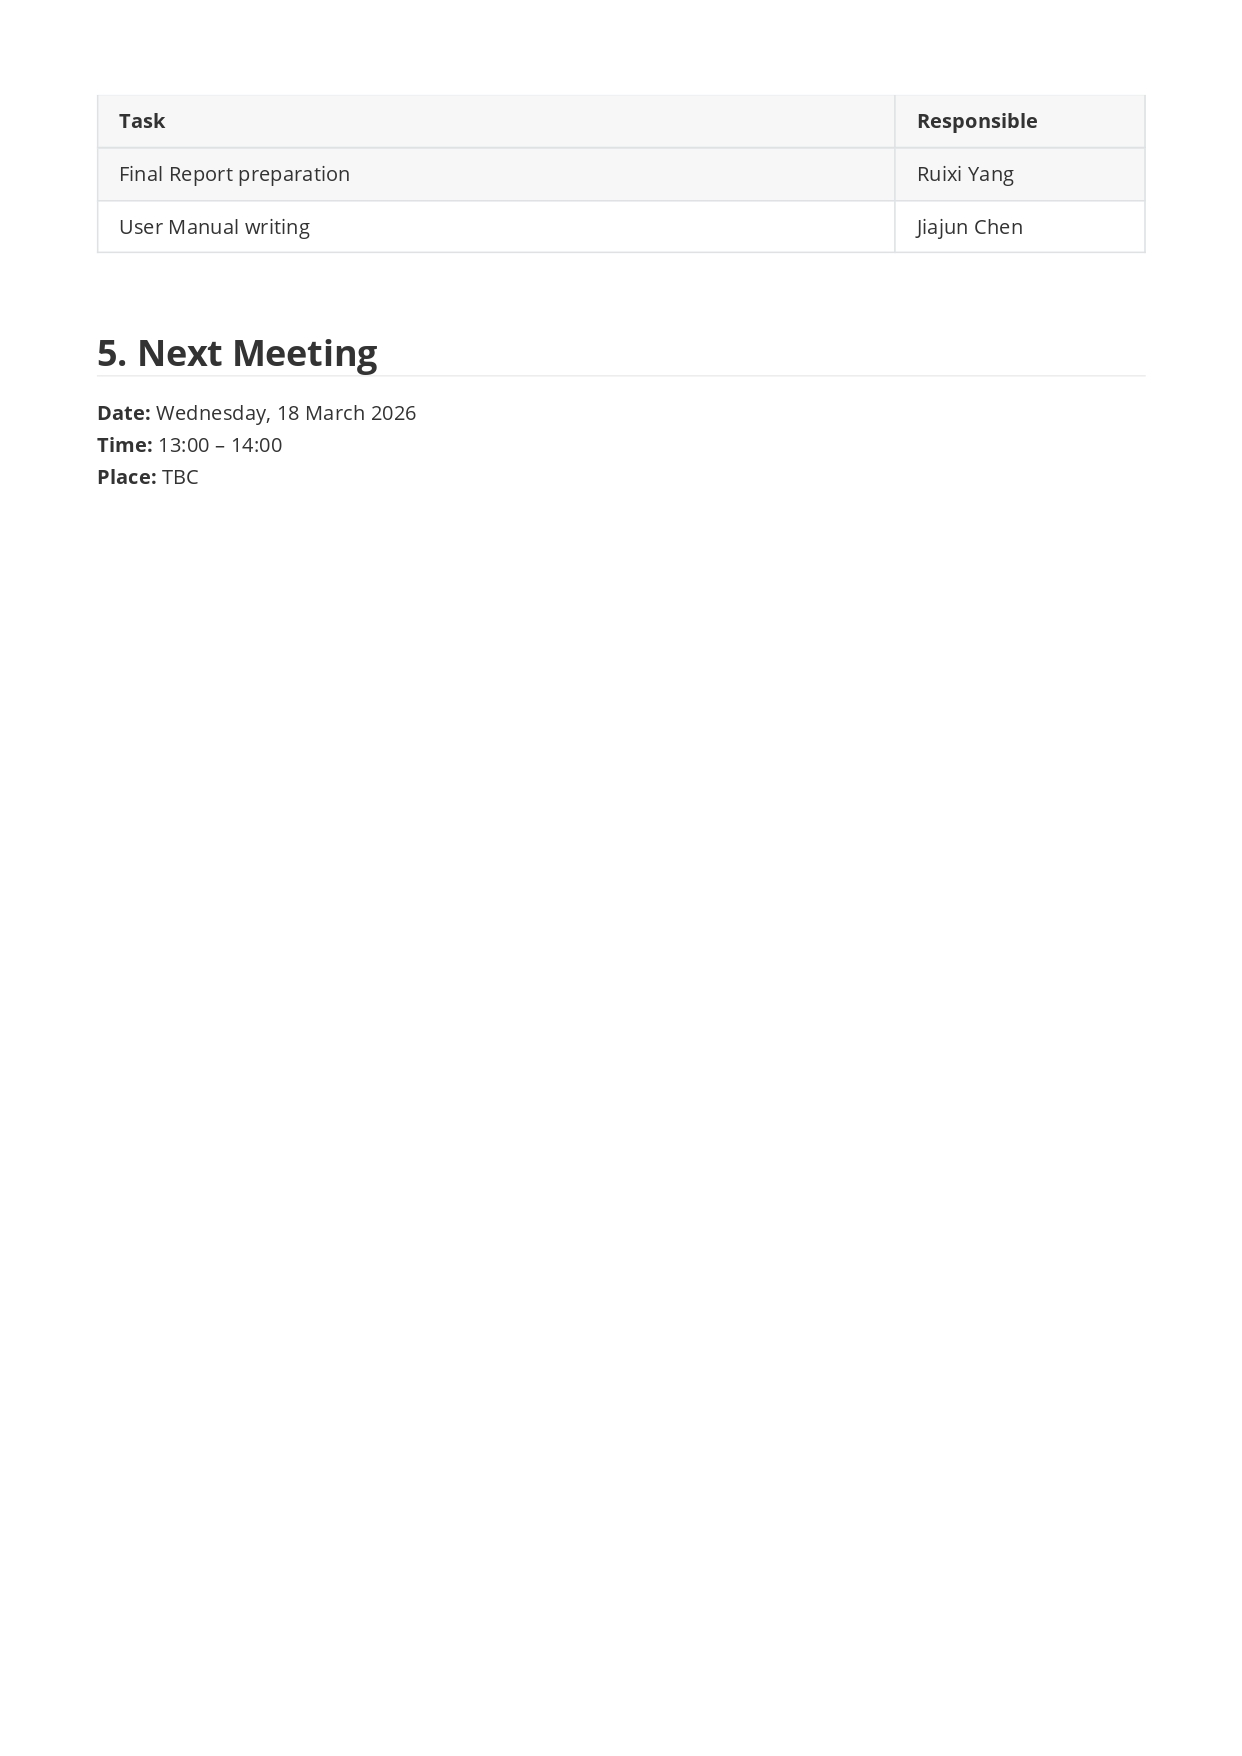
\includegraphics[width=1.0\textwidth]{images/appendix/10th_Informal_Meeting_Minutes_2026-03-14_page-0003.jpg}
\end{figure}




\chapter{Test Cases}
\label{appendix:testing}


\section{Unit Test Cases}
\label{appendix:unit_testing}
The following tables summarize representative unit tests grouped by module. The Actual Result and Status shown below reflect the default outcome when the unit test suite runs successfully.

{\small
\renewcommand{\arraystretch}{1.2}
\setlength{\tabcolsep}{4pt}

\subsection*{Authentication Tests}
\begin{longtable}{|p{1.2cm}|p{3.0cm}|p{2.8cm}|p{3.2cm}|p{2.2cm}|p{1.1cm}|}
\hline
\textbf{ID} & \textbf{Description} & \textbf{Pre-condition} & \textbf{Expected Result} & \textbf{Actual Result} & \textbf{Status} \\
\hline
\endfirsthead
\hline
\textbf{ID} & \textbf{Description} & \textbf{Pre-condition} & \textbf{Expected Result} & \textbf{Actual Result} & \textbf{Status} \\
\hline
\endhead
\hline
\endfoot

JWT-01 &
JWT creation and successful verification &
pytest environment; conftest.py sets fixed SECRET\_KEY &
Decoded payload contains correct sub, user\_id, and exp &
As expected &
Pass \\
\hline

JWT-02 &
Reject malformed JWT input &
Same pre-condition as JWT-01 &
verify\_access\_token returns None &
As expected &
Pass \\
\hline

JWT-03 &
Reject tampered JWT signature &
Valid token generated then last segment altered &
Verification returns None &
As expected &
Pass \\
\hline

JWT-04 &
Reject expired JWT &
Token created with already-expired exp &
verify\_access\_token returns None &
As expected &
Pass \\
\hline

JWT-05 &
Password reset token creation and verification &
Fixed SECRET\_KEY via conftest &
verify\_password\_reset\_token returns the original email &
As expected &
Pass \\
\hline

JWT-06 &
Reject access token as password-reset token &
Valid access token from create\_access\_token &
verify\_password\_reset\_token returns None (wrong type) &
As expected &
Pass \\
\hline

JWT-07 &
Reject expired password-reset token &
Manually encoded JWT with past exp and type reset &
verify\_password\_reset\_token returns None &
As expected &
Pass \\
\hline

PWD-01 &
Password hashing and verification &
None &
Correct password verifies; incorrect password rejected &
As expected &
Pass \\
\hline

DB-01 &
authenticate\_user success with mocked session &
Mock DB returns user; hash matches password &
Returns user and no error string &
As expected &
Pass \\
\hline

DB-02 &
authenticate\_user wrong password &
Mock user with known hash &
Returns None and incorrect-credentials message &
As expected &
Pass \\
\hline

DB-03 &
authenticate\_user unknown user &
Mock session returns no user row &
Returns None and error message &
As expected &
Pass \\
\hline

DEP-01 &
get\_current\_user returns active user &
crud.verify\_access and get\_user\_by\_id patched &
Same user object as mocked DB row &
As expected &
Pass \\
\hline

DEP-02 &
get\_current\_user rejects invalid token &
verify\_access\_token returns None &
HTTP Exception 401 &
As expected &
Pass \\
\hline

DEP-03 &
get\_current\_user rejects payload without user\_id &
Payload missing user\_id &
HTTP Exception 401 &
As expected &
Pass \\
\hline

DEP-04 &
get\_current\_user when user row missing &
get\_user\_by\_id returns None &
HTTP Exception 404 &
As expected &
Pass \\
\hline

DEP-05 &
get\_current\_user rejects inactive account &
User.is\_active is False &
HTTP Exception 403 &
As expected &
Pass \\
\hline

\end{longtable}

\subsection*{Schema Validation Tests}
\begin{longtable}{|p{1.2cm}|p{3.0cm}|p{2.8cm}|p{3.2cm}|p{2.2cm}|p{1.1cm}|}
\hline
\textbf{ID} & \textbf{Description} & \textbf{Pre-condition} & \textbf{Expected Result} & \textbf{Actual Result} & \textbf{Status} \\
\hline
\endfirsthead
\hline
\textbf{ID} & \textbf{Description} & \textbf{Pre-condition} & \textbf{Expected Result} & \textbf{Actual Result} & \textbf{Status} \\
\hline
\endhead
\hline
\endfoot

REG-01 &
UserCreate rejects mismatched passwords &
Pydantic models available &
Validation Error raised &
As expected &
Pass \\
\hline

REG-02 &
UserCreate rejects invalid username characters &
None &
Validation Error raised &
As expected &
Pass \\
\hline

LOGIN-01 &
UserLogin rejects empty username &
None &
Validation Error raised &
As expected &
Pass \\
\hline

RST-01 &
PasswordReset rejects non-matching confirm password &
None &
Validation Error raised &
As expected &
Pass \\
\hline

RST-02 &
PasswordReset trims username &
None &
Username stripped to non-empty token &
As expected &
Pass \\
\hline

WX-01 &
WeatherLatLon coerces string coordinates &
None &
lat/lon parsed as floats &
As expected &
Pass \\
\hline

CHAT-01 &
ChatReq default and non-empty history &
None &
Default empty history; optional history accepted &
As expected &
Pass \\
\hline

\end{longtable}

\subsection*{API Response and Error Types}
\begin{longtable}{|p{1.2cm}|p{3.0cm}|p{2.8cm}|p{3.2cm}|p{2.2cm}|p{1.1cm}|}
\hline
\textbf{ID} & \textbf{Description} & \textbf{Pre-condition} & \textbf{Expected Result} & \textbf{Actual Result} & \textbf{Status} \\
\hline
\endfirsthead
\hline
\textbf{ID} & \textbf{Description} & \textbf{Pre-condition} & \textbf{Expected Result} & \textbf{Actual Result} & \textbf{Status} \\
\hline
\endhead
\hline
\endfoot

API-01 &
success\_body minimal shape &
None &
success true; message ok; status\_code 200; no data key unless set &
As expected &
Pass \\
\hline

API-02 &
success\_body with data and extra fields &
None &
data and extra keys merged into response dict &
As expected &
Pass \\
\hline

API-03 &
error\_body shape &
None &
success false; message and status\_code set &
As expected &
Pass \\
\hline

ERR-01 &
App Error carries message and HTTP status &
None &
exception.message and exception.status\_code match constructor &
As expected &
Pass \\
\hline

\end{longtable}

\subsection*{Wardrobe Module Tests}
\begin{longtable}{|p{1.2cm}|p{3.0cm}|p{2.8cm}|p{3.2cm}|p{2.2cm}|p{1.1cm}|}
\hline
\textbf{ID} & \textbf{Description} & \textbf{Pre-condition} & \textbf{Expected Result} & \textbf{Actual Result} & \textbf{Status} \\
\hline
\endfirsthead
\hline
\textbf{ID} & \textbf{Description} & \textbf{Pre-condition} & \textbf{Expected Result} & \textbf{Actual Result} & \textbf{Status} \\
\hline
\endhead
\hline
\endfoot

NORM-01 &
Normalize clothing category from form input &
conftest stubs heavy AI imports for clothing\_service &
Invalid or blank input is mapped to other; valid category remains unchanged &
As expected &
Pass \\
\hline

SEAS-01 &
Parse and validate season JSON from forms &
None &
Array parsed; empty input mapped to None; invalid JSON raises an error &
As expected &
Pass \\
\hline

CRUD-01 &
Clothing create path rolls back on commit failure &
Mock DB; commit raises Runtime Error &
None item returned, error message generated, and rollback invoked &
As expected &
Pass \\
\hline

GET-01 &
get\_clothing\_item returns matching row &
Mock query returns one ClothingItem &
Same object returned &
As expected &
Pass \\
\hline

GET-02 &
get\_clothing\_item returns None when missing &
Mock query returns None &
None returned &
As expected &
Pass \\
\hline

OUT-01 &
create\_outfit rolls back when clothing not owned &
Mock refresh assigns outfit id; clothing query returns None &
None outfit, error string, rollback called &
As expected &
Pass \\
\hline

\end{longtable}

\subsection*{Context Builder Tests}
\begin{longtable}{|p{1.2cm}|p{3.0cm}|p{2.8cm}|p{3.2cm}|p{2.2cm}|p{1.1cm}|}
\hline
\textbf{ID} & \textbf{Description} & \textbf{Pre-condition} & \textbf{Expected Result} & \textbf{Actual Result} & \textbf{Status} \\
\hline
\endfirsthead
\hline
\textbf{ID} & \textbf{Description} & \textbf{Pre-condition} & \textbf{Expected Result} & \textbf{Actual Result} & \textbf{Status} \\
\hline
\endhead
\hline
\endfoot

CTX-01 &
build\_agent\_context aggregated structure &
DB reader functions patched &
Payload includes user, closet, summary, pagination, and constraints &
As expected &
Pass \\
\hline

CTX-02 &
build\_agent\_context rejects non-positive user\_id &
None &
Value Error raised &
As expected &
Pass \\
\hline

CTX-03 &
build\_agent\_context when user row missing &
\_fetch\_all returns empty list &
Value Error raised for missing user &
As expected &
Pass \\
\hline

CTX-04 &
Retriever serialization and summary helpers &
None &
Enum and decimal fields serialized correctly; counts and recent wear order are correct &
As expected &
Pass \\
\hline

\end{longtable}

\subsection*{Language Policy Tests}
\begin{longtable}{|p{1.2cm}|p{3.0cm}|p{2.8cm}|p{3.2cm}|p{2.2cm}|p{1.1cm}|}
\hline
\textbf{ID} & \textbf{Description} & \textbf{Pre-condition} & \textbf{Expected Result} & \textbf{Actual Result} & \textbf{Status} \\
\hline
\endfirsthead
\hline
\textbf{ID} & \textbf{Description} & \textbf{Pre-condition} & \textbf{Expected Result} & \textbf{Actual Result} & \textbf{Status} \\
\hline
\endhead
\hline
\endfoot

LANG-01 &
Detect Chinese- vs English-dominant text &
None &
zh or en detection matches the input language dominance &
As expected &
Pass \\
\hline

LANG-02 &
Short English acknowledgement follows Chinese context &
History includes Chinese user turn &
decide\_reply\_language returns zh &
As expected &
Pass \\
\hline

LANG-03 &
Explicit Chinese query selects zh &
None &
Returns zh &
As expected &
Pass \\
\hline

\end{longtable}

\subsection*{LLM Message Processing Tests}
\begin{longtable}{|p{1.2cm}|p{3.0cm}|p{2.8cm}|p{3.2cm}|p{2.2cm}|p{1.1cm}|}
\hline
\textbf{ID} & \textbf{Description} & \textbf{Pre-condition} & \textbf{Expected Result} & \textbf{Actual Result} & \textbf{Status} \\
\hline
\endfirsthead
\hline
\textbf{ID} & \textbf{Description} & \textbf{Pre-condition} & \textbf{Expected Result} & \textbf{Actual Result} & \textbf{Status} \\
\hline
\endhead
\hline
\endfoot

LLM-01 &
Plain-text assistant message (no JSON) &
None &
renderType is text &
As expected &
Pass \\
\hline

LLM-02 &
Invalid JSON string fallback &
None &
renderType is text &
As expected &
Pass \\
\hline

LLM-03 &
Normalize LLM recommendation JSON &
Valid JSON with mixed item types and empty names &
Types normalized, empty names skipped, and locale set to zh &
As expected &
Pass \\
\hline

LLM-04 &
Plan payload preferred when both plan and recommendations exist &
JSON includes plan.days and recommendations &
renderType is plan &
As expected &
Pass \\
\hline

LLM-05 &
Whitespace-only recommendation title skipped &
JSON with blank title &
Falls back to text mode &
As expected &
Pass \\
\hline

LLM-06 &
Unsupported locale defaults to English &
JSON with unknown locale &
Output locale is en &
As expected &
Pass \\
\hline

\end{longtable}

\subsection*{Weather and Wind Scale Tests}
\begin{longtable}{|p{1.2cm}|p{3.0cm}|p{2.8cm}|p{3.2cm}|p{2.2cm}|p{1.1cm}|}
\hline
\textbf{ID} & \textbf{Description} & \textbf{Pre-condition} & \textbf{Expected Result} & \textbf{Actual Result} & \textbf{Status} \\
\hline
\endfirsthead
\hline
\textbf{ID} & \textbf{Description} & \textbf{Pre-condition} & \textbf{Expected Result} & \textbf{Actual Result} & \textbf{Status} \\
\hline
\endhead
\hline
\endfoot

WXF-01 &
Weather observation freshness within 30 minutes &
Test uses fixed reference time consistent with the production rule &
Returns True for fresh obsTime &
As expected &
Pass \\
\hline

WXF-02 &
Stale observation marked not fresh &
Fixed reference time; old obsTime &
Returns False &
As expected &
Pass \\
\hline

WXF-03 &
Missing observation time not fresh &
Payload without now.obsTime &
Returns False &
As expected &
Pass \\
\hline

WND-01 &
Wind scale description mapping (breeze bands) &
weather\_service module loaded &
Scale 0--2 maps to Light Breeze; mid values to Moderate/Strong Breeze &
As expected &
Pass \\
\hline

WND-02 &
Wind scale description mapping (gale and storm) &
None &
High scales map to Gale or Storm &
As expected &
Pass \\
\hline

WND-03 &
Wind scale invalid input &
Non-integer scale string &
Returns em dash placeholder &
As expected &
Pass \\
\hline

\end{longtable}

\subsection*{Virtual Try-on Workflow Tests}
\begin{longtable}{|p{1.2cm}|p{3.0cm}|p{2.8cm}|p{3.2cm}|p{2.2cm}|p{1.1cm}|}
\hline
\textbf{ID} & \textbf{Description} & \textbf{Pre-condition} & \textbf{Expected Result} & \textbf{Actual Result} & \textbf{Status} \\
\hline
\endfirsthead
\hline
\textbf{ID} & \textbf{Description} & \textbf{Pre-condition} & \textbf{Expected Result} & \textbf{Actual Result} & \textbf{Status} \\
\hline
\endhead
\hline
\endfoot

VTO-01 &
Map images into ComfyUI workflow template &
Template qwen\_edit\_v1.json present under app/resources &
Person, clothing, and accessory filenames are mapped to the expected nodes &
As expected &
Pass \\
\hline

VTO-02 &
clean\_token strips quotes and whitespace &
None &
None input yields empty string; wrapped tokens normalized &
As expected &
Pass \\
\hline

\end{longtable}
}



\section{Integration Test Cases}
\label{appendix:integration_testing}

{\small
\renewcommand{\arraystretch}{1.2}
\setlength{\tabcolsep}{4pt}

\subsection*{Authentication API (HTTP)}
\begin{longtable}{|p{1.2cm}|p{3.0cm}|p{3.0cm}|p{3.2cm}|p{2.2cm}|p{1.1cm}|}
\hline
\textbf{ID} & \textbf{Description} & \textbf{Pre-condition} & \textbf{Expected Result} & \textbf{Actual Result} & \textbf{Status} \\
\hline
\endfirsthead
\hline
\textbf{ID} & \textbf{Description} & \textbf{Pre-condition} & \textbf{Expected Result} & \textbf{Actual Result} & \textbf{Status} \\
\hline
\endhead
\hline
\endfoot

AUT-01 &
POST /api/auth/register returns user payload &
auth\_app; crud.create\_user patched to succeed &
HTTP 200; success true; data contains username and id &
As expected &
Pass \\
\hline

AUT-02 &
POST /api/auth/register conflict returns 409 &
create\_user returns error tuple (username taken) &
HTTP 409; success false &
As expected &
Pass \\
\hline

AUT-03 &
POST /api/auth/login returns access token &
authenticate\_user and create\_access\_token patched &
HTTP 200; success true; access\_token and user\_id present &
As expected &
Pass \\
\hline

AUT-04 &
POST /api/auth/login invalid credentials envelope &
authenticate\_user returns None with error message &
HTTP 200; success false; status\_code 401 in JSON body &
As expected &
Pass \\
\hline

AUT-05 &
GET /api/auth/verify accepts valid token &
verify\_access\_token and get\_user\_by\_id patched &
HTTP 200; valid true; username matches mock user &
As expected &
Pass \\
\hline

AUT-06 &
GET /api/auth/verify rejects invalid token &
verify\_access\_token returns None &
HTTP 401 &
As expected &
Pass \\
\hline

\end{longtable}

\subsection*{Password Reset by Identity API (HTTP)}
\begin{longtable}{|p{1.2cm}|p{3.0cm}|p{3.0cm}|p{3.2cm}|p{2.2cm}|p{1.1cm}|}
\hline
\textbf{ID} & \textbf{Description} & \textbf{Pre-condition} & \textbf{Expected Result} & \textbf{Actual Result} & \textbf{Status} \\
\hline
\endfirsthead
\hline
\textbf{ID} & \textbf{Description} & \textbf{Pre-condition} & \textbf{Expected Result} & \textbf{Actual Result} & \textbf{Status} \\
\hline
\endhead
\hline
\endfoot

RST-01 &
POST /api/auth/reset-password-by-identity success &
get\_user\_by\_username and update\_user\_password patched; email matches user &
HTTP 200; success true &
As expected &
Pass \\
\hline

RST-02 &
POST /api/auth/reset-password-by-identity email mismatch &
User row email differs from request body &
HTTP 400 &
As expected &
Pass \\
\hline

\end{longtable}

\subsection*{User Profile API (HTTP)}
\begin{longtable}{|p{1.2cm}|p{3.0cm}|p{3.0cm}|p{3.2cm}|p{2.2cm}|p{1.1cm}|}
\hline
\textbf{ID} & \textbf{Description} & \textbf{Pre-condition} & \textbf{Expected Result} & \textbf{Actual Result} & \textbf{Status} \\
\hline
\endfirsthead
\hline
\textbf{ID} & \textbf{Description} & \textbf{Pre-condition} & \textbf{Expected Result} & \textbf{Actual Result} & \textbf{Status} \\
\hline
\endhead
\hline
\endfoot

USR-01 &
GET /api/users/me returns profile &
users\_app; verify\_access\_token and get\_user\_by\_id patched &
HTTP 200; username and id match mock user &
As expected &
Pass \\
\hline

USR-02 &
PATCH /api/users/me updates via crud &
get\_current\_user and crud.update\_user patched &
HTTP 200; body reflects updated user fields &
As expected &
Pass \\
\hline

\end{longtable}

\subsection*{Recommendation AI Conversations API (HTTP)}
\begin{longtable}{|p{1.2cm}|p{3.0cm}|p{3.0cm}|p{3.2cm}|p{2.2cm}|p{1.1cm}|}
\hline
\textbf{ID} & \textbf{Description} & \textbf{Pre-condition} & \textbf{Expected Result} & \textbf{Actual Result} & \textbf{Status} \\
\hline
\endfirsthead
\hline
\textbf{ID} & \textbf{Description} & \textbf{Pre-condition} & \textbf{Expected Result} & \textbf{Actual Result} & \textbf{Status} \\
\hline
\endhead
\hline
\endfoot

AIC-01 &
GET /api/ai/conversations lists conversations &
ai\_chat\_app; get\_current\_user and list\_by\_user patched &
HTTP 200; success true; data array and total consistent &
As expected &
Pass \\
\hline

AIC-02 &
POST /api/ai/conversations creates conversation &
create patched to return new conversation row &
HTTP 200; success true; data.id matches mock &
As expected &
Pass \\
\hline

AIC-03 &
DELETE /api/ai/conversations/\{id\} succeeds &
delete patched to return success &
HTTP 200; success true &
As expected &
Pass \\
\hline

\end{longtable}

\subsection*{Recommendation AI Chat Stream API (HTTP)}
\begin{longtable}{|p{1.2cm}|p{3.0cm}|p{3.0cm}|p{3.2cm}|p{2.2cm}|p{1.1cm}|}
\hline
\textbf{ID} & \textbf{Description} & \textbf{Pre-condition} & \textbf{Expected Result} & \textbf{Actual Result} & \textbf{Status} \\
\hline
\endfirsthead
\hline
\textbf{ID} & \textbf{Description} & \textbf{Pre-condition} & \textbf{Expected Result} & \textbf{Actual Result} & \textbf{Status} \\
\hline
\endhead
\hline
\endfoot

STR-01 &
POST /api/ai/chat/stream rejects blank query (SSE) &
Stream request with whitespace-only query &
HTTP 200; SSE body contains error type and empty-message wording &
As expected &
Pass \\
\hline

STR-02 &
POST /api/ai/chat/stream yields delta, final, done &
ReactAgent.execute patched to yield text chunk &
SSE contains delta, final, and done events &
As expected &
Pass \\
\hline

\end{longtable}

\subsection*{Clothing List API (HTTP)}
\begin{longtable}{|p{1.2cm}|p{3.0cm}|p{3.0cm}|p{3.2cm}|p{2.2cm}|p{1.1cm}|}
\hline
\textbf{ID} & \textbf{Description} & \textbf{Pre-condition} & \textbf{Expected Result} & \textbf{Actual Result} & \textbf{Status} \\
\hline
\endfirsthead
\hline
\textbf{ID} & \textbf{Description} & \textbf{Pre-condition} & \textbf{Expected Result} & \textbf{Actual Result} & \textbf{Status} \\
\hline
\endhead
\hline
\endfoot

CLO-01 &
GET /api/clothing empty list and pagination &
get\_current\_user and get\_clothing\_items return empty &
HTTP 200; success true; items empty; total 0 &
As expected &
Pass \\
\hline

CLO-02 &
GET /api/clothing passes search and filters to CRUD &
Same mocks; request includes search, category, season &
get\_clothing\_items called with matching keyword arguments &
As expected &
Pass \\
\hline
\end{longtable}

\subsection*{Calendar and Analysis API (HTTP)}
\begin{longtable}{|p{1.2cm}|p{3.0cm}|p{3.0cm}|p{3.2cm}|p{2.2cm}|p{1.1cm}|}
\hline
\textbf{ID} & \textbf{Description} & \textbf{Pre-condition} & \textbf{Expected Result} & \textbf{Actual Result} & \textbf{Status} \\
\hline
\endfirsthead
\hline
\textbf{ID} & \textbf{Description} & \textbf{Pre-condition} & \textbf{Expected Result} & \textbf{Actual Result} & \textbf{Status} \\
\hline
\endhead
\hline
\endfoot

CAL-01 &
GET /api/calendar/outfits empty month &
calendar\_app; get\_current\_user and DB query chain return no rows &
HTTP 200; success true; outfits empty; monthStats zeros &
As expected &
Pass \\
\hline

ANA-01 &
GET /api/analysis/total-items/summary &
analysis\_app; get\_current\_user and run\_total\_items\_summary patched &
HTTP 200; JSON equals mocked summary payload &
As expected &
Pass \\
\hline

\end{longtable}

\subsection*{Model Photos API (HTTP)}
\begin{longtable}{|p{1.2cm}|p{3.0cm}|p{3.0cm}|p{3.2cm}|p{2.2cm}|p{1.1cm}|}
\hline
\textbf{ID} & \textbf{Description} & \textbf{Pre-condition} & \textbf{Expected Result} & \textbf{Actual Result} & \textbf{Status} \\
\hline
\endfirsthead
\hline
\textbf{ID} & \textbf{Description} & \textbf{Pre-condition} & \textbf{Expected Result} & \textbf{Actual Result} & \textbf{Status} \\
\hline
\endhead
\hline
\endfoot

MOD-01 &
POST /api/model-photos/upload success &
model\_photos\_app; get\_current\_user, save\_upload\_file, create\_model\_photo patched &
HTTP 200; success true; data.id present &
As expected &
Pass \\
\hline

\end{longtable}

\subsection*{Weather API (HTTP)}
\begin{longtable}{|p{1.2cm}|p{3.0cm}|p{3.0cm}|p{3.2cm}|p{2.2cm}|p{1.1cm}|}
\hline
\textbf{ID} & \textbf{Description} & \textbf{Pre-condition} & \textbf{Expected Result} & \textbf{Actual Result} & \textbf{Status} \\
\hline
\endfirsthead
\hline
\textbf{ID} & \textbf{Description} & \textbf{Pre-condition} & \textbf{Expected Result} & \textbf{Actual Result} & \textbf{Status} \\
\hline
\endhead
\hline
\endfoot

WEA-01 &
GET /api/weather/now delegates to service &
weather\_app; fetch\_weather\_now patched &
HTTP 200; JSON contains mocked temp; service called once &
As expected &
Pass \\
\hline

\end{longtable}

\subsection*{Virtual Try-on API (HTTP)}
\begin{longtable}{|p{1.2cm}|p{3.0cm}|p{3.0cm}|p{3.2cm}|p{2.2cm}|p{1.1cm}|}
\hline
\textbf{ID} & \textbf{Description} & \textbf{Pre-condition} & \textbf{Expected Result} & \textbf{Actual Result} & \textbf{Status} \\
\hline
\endfirsthead
\hline
\textbf{ID} & \textbf{Description} & \textbf{Pre-condition} & \textbf{Expected Result} & \textbf{Actual Result} & \textbf{Status} \\
\hline
\endhead
\hline
\endfoot

VTO-01 &
POST /api/virtual-try-on/generate returns PNG &
virtual\_tryon\_app; run\_generate returns PngBytesResult &
HTTP 200; Content-Type image/png &
As expected &
Pass \\
\hline

VTO-02 &
POST /api/virtual-try-on/generate error returns JSON envelope &
Service returns JsonEnvelope with 400 &
HTTP 400; success false in body &
As expected &
Pass \\
\hline

VTO-03 &
POST /api/virtual-try-on/upload-image returns envelope &
run\_upload\_image patched (async) &
HTTP 200; success true in JSON &
As expected &
Pass \\
\hline

\end{longtable}
}


\section{System Test Cases}
\label{appendix:system_testing}


\begin{landscape}
\subsection*{Authentication}

\begin{longtable}{|p{0.6cm}|p{2.8cm}|p{2.5cm}|p{6cm}|p{5cm}|p{1.2cm}|p{1.8cm}|}
\hline
\textbf{ID} & \textbf{Test Focus} & \textbf{Precondition} & \textbf{Test Steps} & \textbf{Expected Result} & \textbf{Prio} & \textbf{Type} \\
\hline

01 & Valid login & User registered & Open login page; enter test01 and 123456; click login & Login successful, redirect to homepage & P0 & Functional \\
\hline
02 & Wrong password & User registered & Enter test01 and wrong; click login & Error message shown & P1 & Functional \\
\hline
03 & Empty username & - & Leave username empty; click login & Prompt to enter username & P2 & UI \\
\hline
04 & Empty password & - & Leave password empty; click login & Prompt to enter password & P2 & UI \\
\hline
05 & Password toggle & User registered & Enter password; click eye icon & Password becomes visible & P2 & UI \\
\hline
06 & Successful registration & Username unused & Enter newuser / 123456; submit & Registration success & P0 & Functional \\
\hline
07 & Duplicate account & Username exists & Use existing account & Error shown & P1 & Functional \\
\hline
08 & Password mismatch & - & Enter different passwords & Error shown & P1 & Functional \\
\hline
09 & Invalid email & - & Enter invalid email & Prompt shown & P1 & Functional \\
\hline
10 & Empty form & - & Submit empty form & Prompt required fields & P2 & UI \\
\hline

\end{longtable}
\end{landscape}


\begin{landscape}
\subsection*{Wardrobe Management}

\begin{longtable}{|p{0.8cm}|p{2.8cm}|p{3.5cm}|p{5cm}|p{5cm}|p{1.2cm}|p{1.8cm}|}
\hline
\textbf{ID} & \textbf{Test Focus} & \textbf{Precondition} & \textbf{Test Steps} & \textbf{Expected Result} & \textbf{Prio} & \textbf{Type} \\
\hline

01 & Upload single image & User logged in & Go to wardrobe page; click upload; select image: white\_shirt.jpg; select category: shirt; add description: white shirt & Image uploaded successfully, shows at top of the list & P0 & Functional \\
\hline
02 & Upload non-image file & User logged in & Click upload; select PDF file: test.pdf & Error message "Please select an image file (jpg/png/jpeg)" & P2 & Exception \\
\hline
03 & Upload oversized image & User logged in & Click upload; select image larger than 20MB: large.jpg & Error message "File size cannot exceed 10MB" & P2 & Performance \\
\hline
04 & Cancel upload & User logged in & Click upload; select image; click cancel during upload & Upload canceled, wardrobe list unchanged & P2 & Functional \\
\hline
05 & Delete single item & Item exists in wardrobe  & Click on item in wardrobe list; click delete; confirm deletion & Item removed from list, count reduced by 1 & P0 & Functional \\
\hline
06 & Cancel delete operation & Item exists in wardrobe & Click delete on item; click cancel in confirmation window & Item remains in the list, count unchanged & P2 & Functional \\
\hline
07 & Filter by category & Wardrobe contains shirts, t-shirts, pants (2 each) & Click on category filter; select "T-shirt" & Only t-shirts shown (2 items) & P1 & Functional \\
\hline
08 & Multi-condition filter & Wardrobe contains various items & Select category: shirt; select color: white; click filter & Only white shirts shown & P1 & Functional \\
\hline
09 & Edit item information & Item exists in wardrobe & Change category to "jacket"; change description to "black jacket" & Item info updated successfully, new category and description shown & P1 & Functional \\
\hline
\end{longtable}
\end{landscape}

\begin{landscape}
\subsection*{Recommendation System}

\begin{longtable}{|p{0.8cm}|p{2.8cm}|p{2.5cm}|p{6cm}|p{5cm}|p{1.2cm}|p{1.8cm}|}
\hline
\textbf{ID} & \textbf{Test Focus} & \textbf{Precondition} & \textbf{Test Steps} & \textbf{Expected Result} & \textbf{Prio} & \textbf{Type} \\
\hline

01 & Recommend outfit for new user & User has no wardrobe data & Request outfit recommendation & Complete outfit recommendation returned (online sources) & P1 & Functional \\
\hline
02 & Recommend outfit from wardrobe data & User has wardrobe data & Request outfit recommendation & Complete outfit recommendation (mix of online images and user wardrobe items) & P0 & Functional \\
\hline
03 & Recommend for business occasion & - & Request business attire recommendation & Business-style outfit recommended & P1 & AI \\
\hline
04 & Recommend for weather conditions & - & Request outfit recommendation for rainy weather & Outfit includes umbrella or waterproof clothing & P1 & AI \\
\hline
05 & Recommend for season & - & Request winter outfit recommendation & Outfit includes warm clothing (e.g., jacket, sweater) & P1 & AI \\
\hline
\end{longtable}
\end{landscape}

\begin{landscape}
\subsection*{Virtual Try-On}

\begin{longtable}{|p{0.8cm}|p{2.8cm}|p{2.5cm}|p{6cm}|p{5cm}|p{1.2cm}|p{1.8cm}|}
\hline
\textbf{ID} & \textbf{Test Focus} & \textbf{Precondition} & \textbf{Test Steps} & \textbf{Expected Result} & \textbf{Prio} & \textbf{Type} \\
\hline

01 & Generate try-on for user & User logged in; wardrobe has clothing & Go to virtual try-on page; select model image (model.jpg); select shirt from wardrobe (shirt\_001); click generate & Display generated try-on image, clear and natural output & P0 & AI \\
\hline
02 & Generate try-on without clothing selection & User logged in & Upload model image (model.jpg); leave clothing unselected; click generate & Error message "Please select a clothing item" & P2 & Functional \\
\hline
03 & Evaluate try-on quality & - & Generate try-on image; evaluate visual quality & Clothing edges natural, good color blending, no distortion & P2 & AI \\
\hline
04 & Adapt try-on for different body types & - & Upload images of different body types (thin/fat/tall/short); use the same clothing item for try-on & Clothing adapts well to different body types & P2 & AI \\
\hline
05 & Performance of try-on generation & - & Upload image; select clothing; click generate & Generation time $\leq$ 10 seconds & P2 & Performance \\
\hline
\end{longtable}
\end{landscape}

\begin{landscape}
\subsection*{Weather Integration}

\begin{longtable}{|p{0.8cm}|p{2.8cm}|p{2.5cm}|p{6cm}|p{5cm}|p{1.2cm}|p{1.8cm}|}
\hline
\textbf{ID} & \textbf{Test Focus} & \textbf{Precondition} & \textbf{Test Steps} & \textbf{Expected Result} & \textbf{Prio} & \textbf{Type} \\
\hline

01 & Display current weather & Location permission granted & Go to chat page; check top weather display & Display current city, temperature, weather status, humidity & P1 & Functional \\
\hline
02 & Handle invalid city name & Location permission denied & Go to chat page; check weather display & Error message "City not found" & P2 & Exception \\
\hline
03 & Auto-refresh weather & Weather data fetched & Stay on page for 30 minutes; observe weather info update & Weather info auto-updates & P2 & Functional \\
\hline
04 & Chat integration with weather & Rainy weather fetched & Enter "What should I wear today?" in chat; send message & Response includes "It's rainy, bring an umbrella" & P1 & AI \\
\hline
\end{longtable}
\end{landscape}

\begin{landscape}
\subsection*{Wardrobe Analysis}

\begin{longtable}{|p{0.8cm}|p{2.8cm}|p{3cm}|p{5.5cm}|p{5cm}|p{1.2cm}|p{1.8cm}|}
\hline
\textbf{ID} & \textbf{Test Focus} & \textbf{Precondition} & \textbf{Test Steps} & \textbf{Expected Result} & \textbf{Prio} & \textbf{Type} \\
\hline

01 & Wardrobe category statistics & Wardrobe contains 10 items & Go to analysis page; view category stats & Show number and percentage for each category (pie/bar chart) & P1 & Functional \\
\hline
02 & Update after upload & Wardrobe empty initially & Upload t-shirt; return to analysis page; refresh & T-shirt count shows 1, total count shows 1 & P0 & Functional \\
\hline
03 & Update after delete & Wardrobe contains 3 items & Delete 1 shirt; return to analysis page; refresh & T-shirt count reduced by 1, total count reduced by 1 & P1 & Functional \\
\hline
04 & Color distribution statistics & Wardrobe contains white (3), black (2), blue (1) & Go to analysis page; view color distribution & Show counts for each color (3 white, 2 black, 1 blue) & P2 & AI \\
\hline
05 & Automatic color recognition & Upload red coat & Go to analysis page; view color stats & Red color count increased by 1 & P2 & AI \\
\hline
\end{longtable}
\end{landscape}

\chapter{Ethics Checklist}
\begin{figure}[H]
    \centering
    
\includegraphics[width=1.0\textwidth]{images/appendix/ethics/Team.202513.FullChecklist_page-0001.jpg}
\end{figure}
\begin{figure}[H]
    \centering
    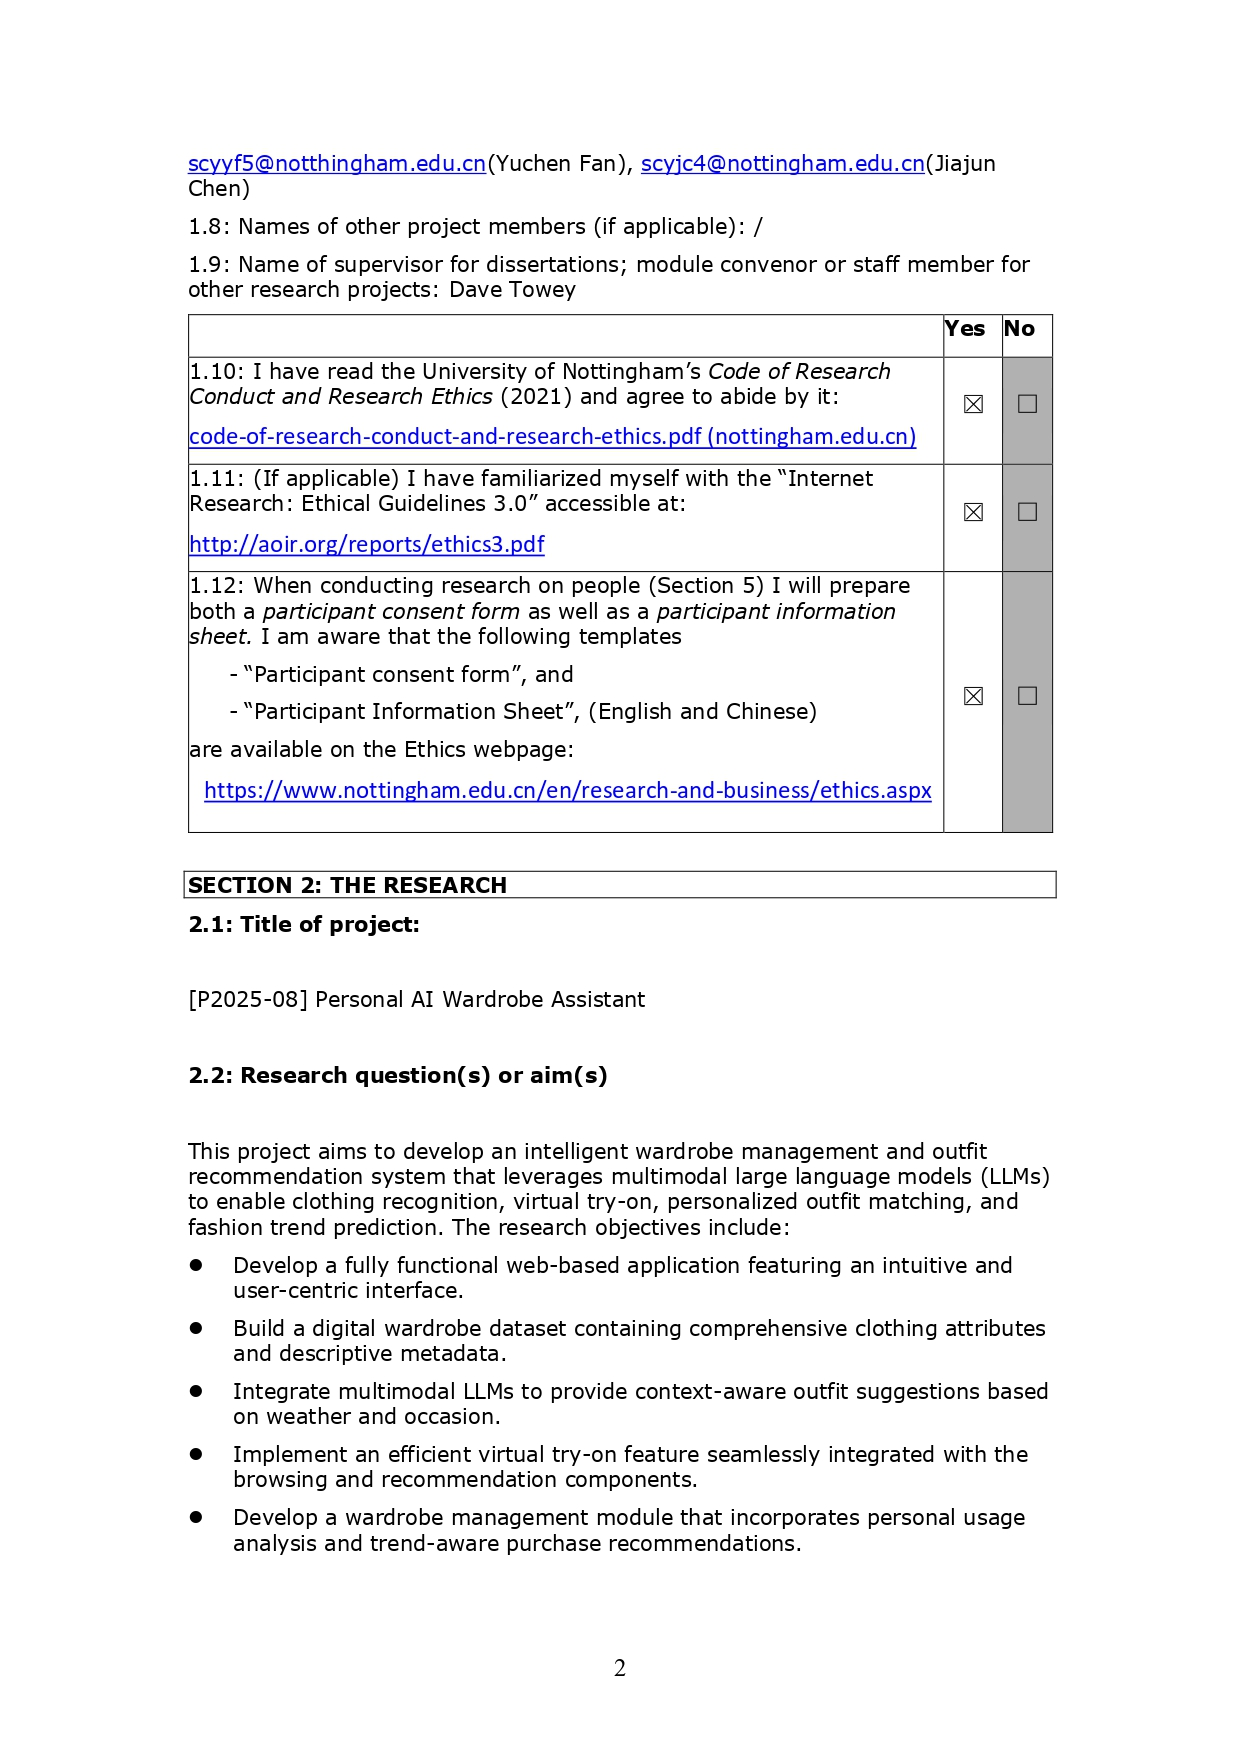
\includegraphics[width=1.0\textwidth]{images/appendix/ethics/Team.202513.FullChecklist_page-0002.jpg}
\end{figure}
\begin{figure}[H]
    \centering
    
\includegraphics[width=1.0\textwidth]{images/appendix/ethics/Team.202513.FullChecklist_page-0003.jpg}
\end{figure}
\begin{figure}[H]
    \centering
    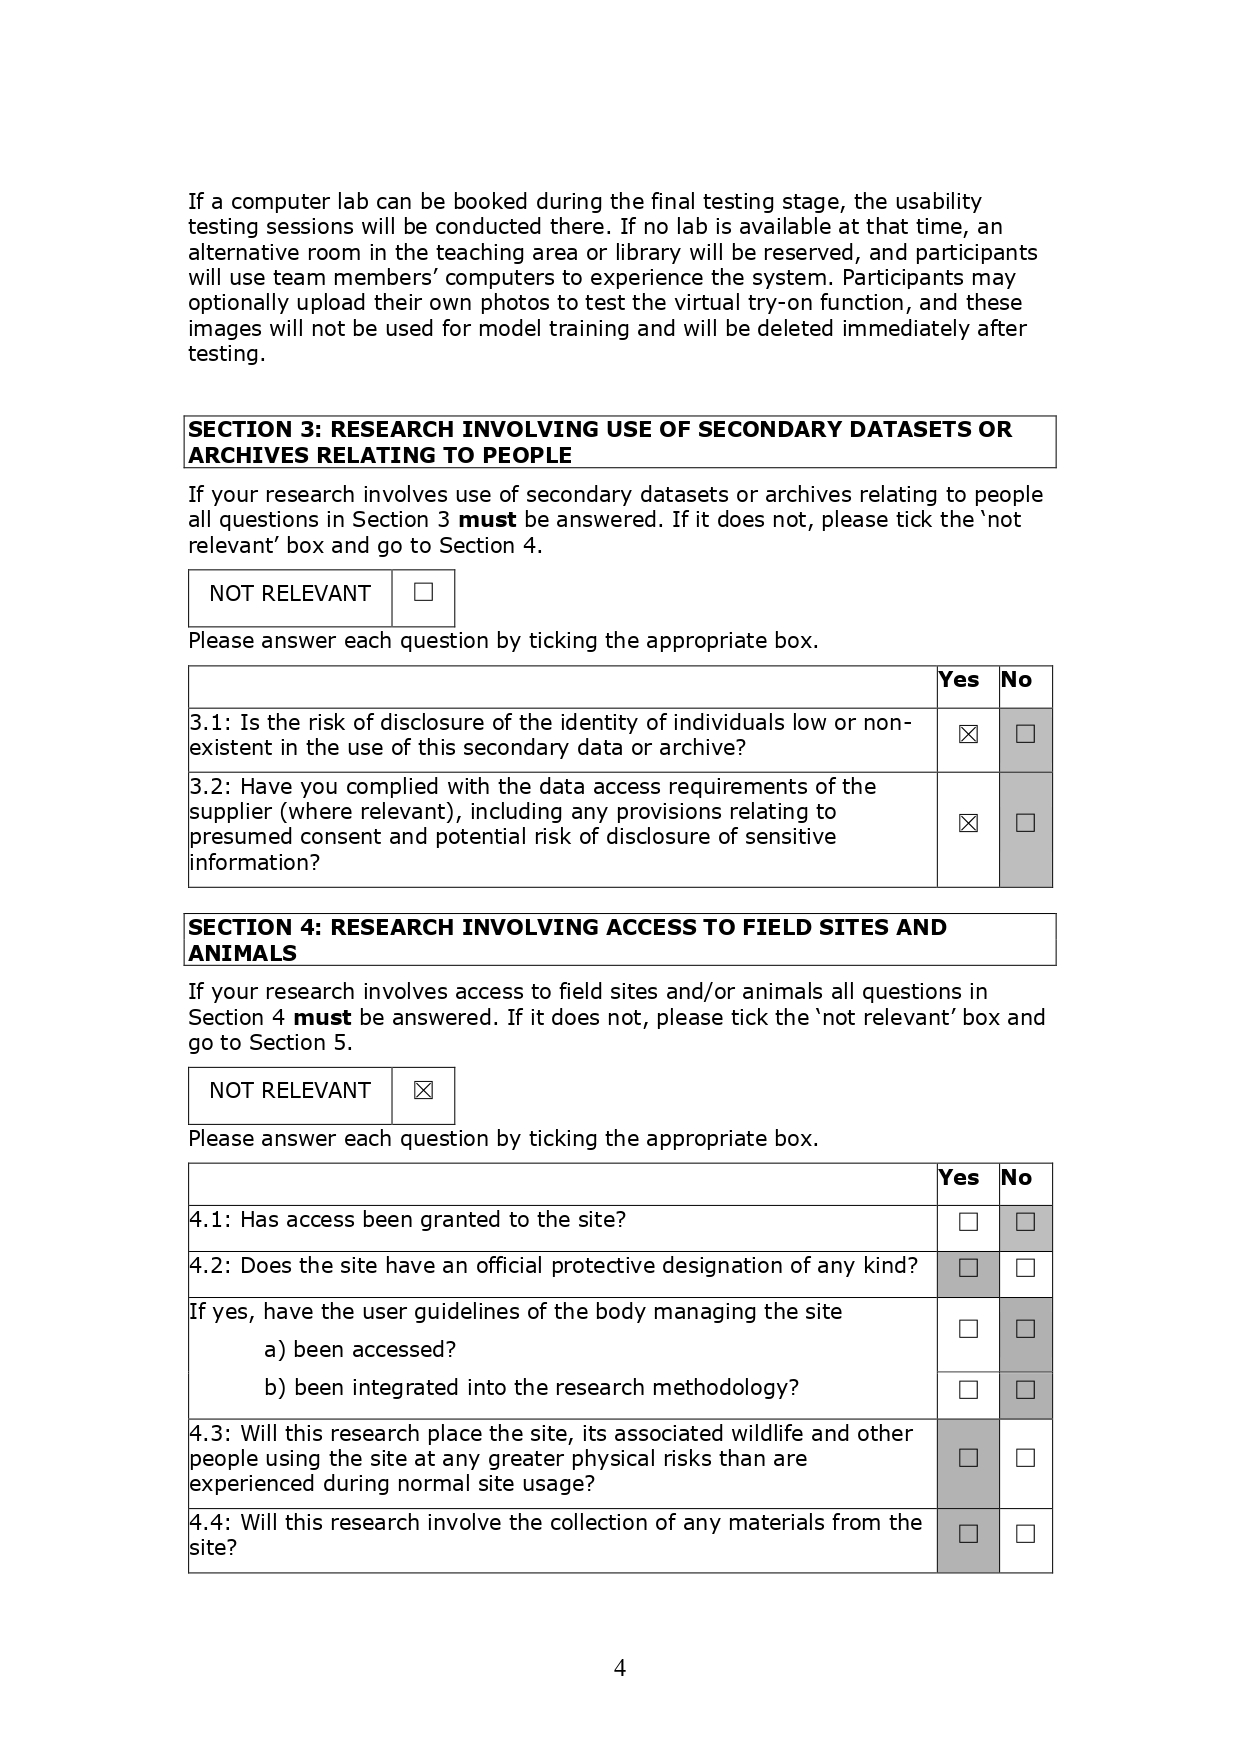
\includegraphics[width=1.0\textwidth]{images/appendix/ethics/Team.202513.FullChecklist_page-0004.jpg}
\end{figure}
\begin{figure}[H]
    \centering
    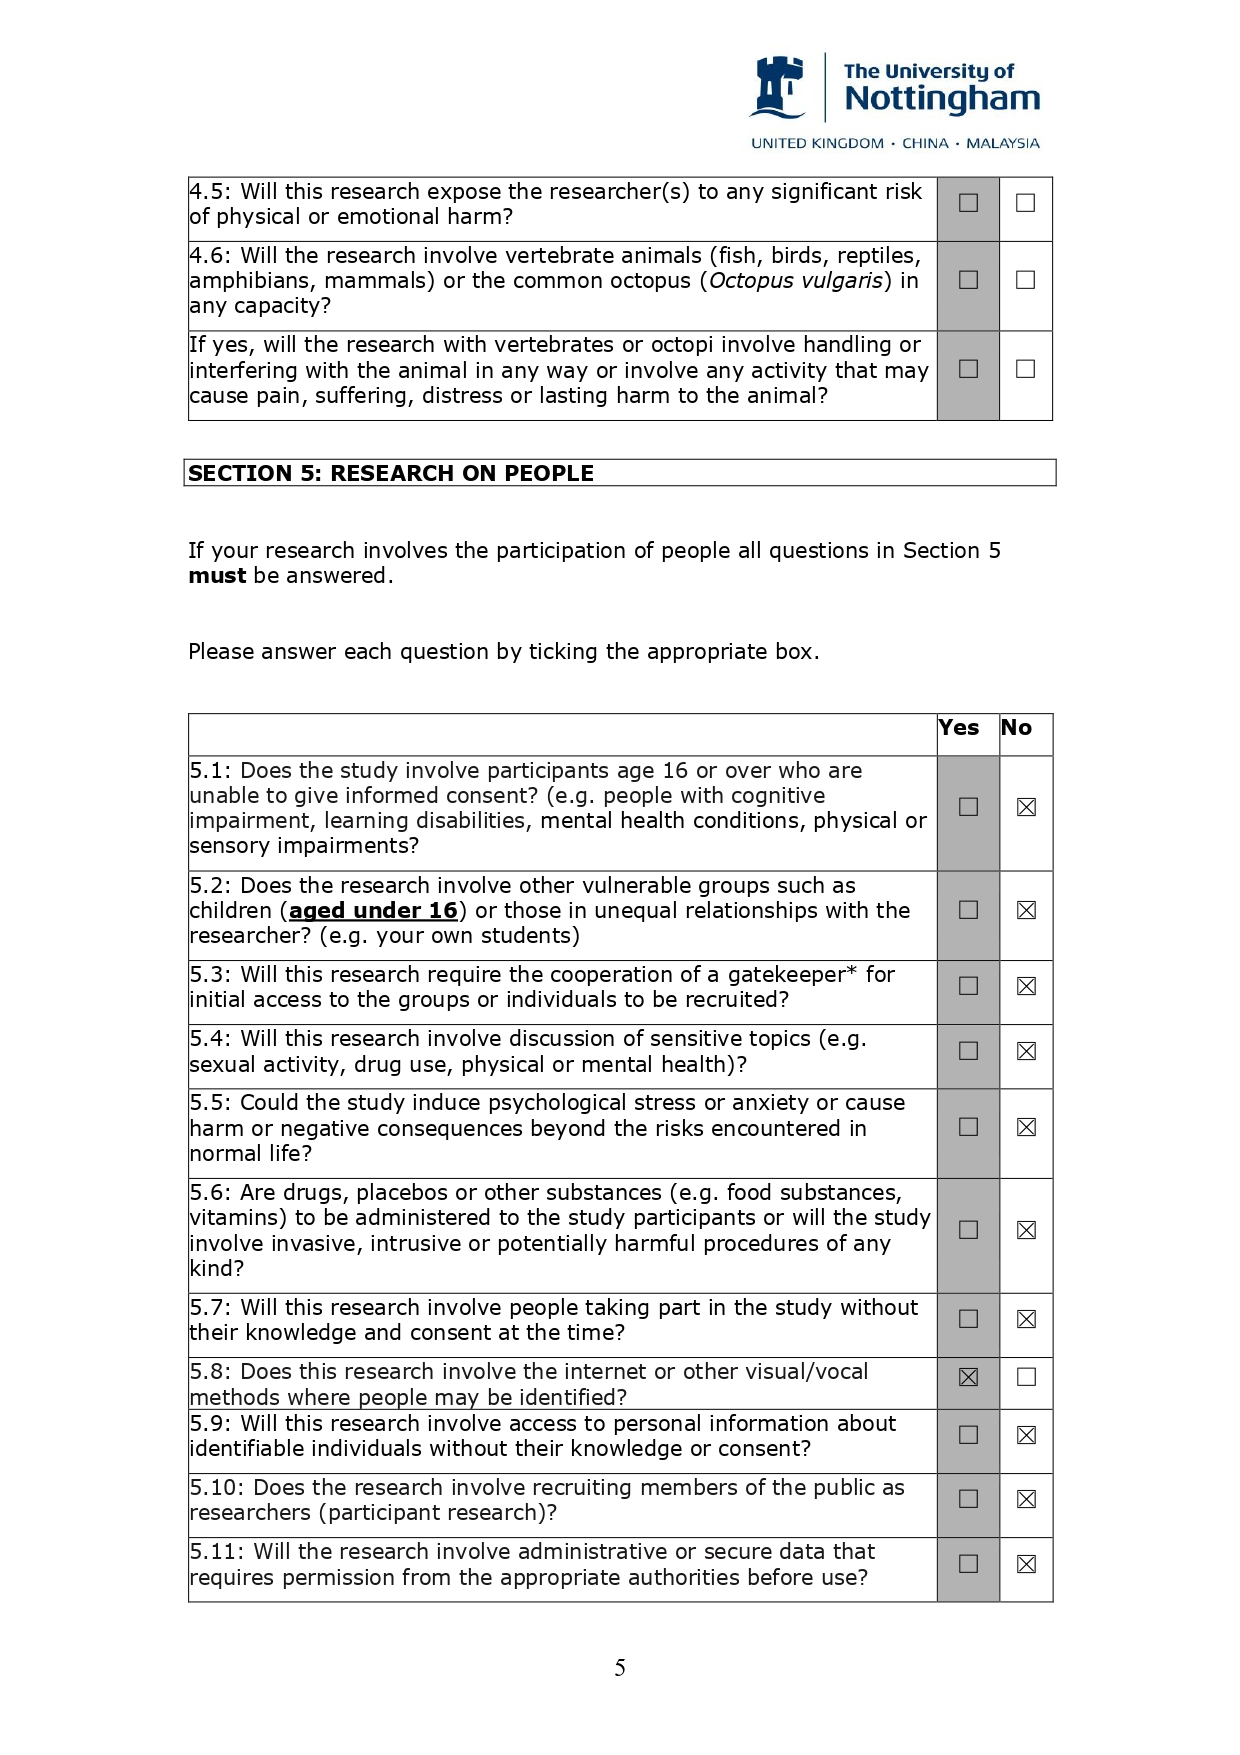
\includegraphics[width=1.0\textwidth]{images/appendix/ethics/Team.202513.FullChecklist_page-0005.jpg}
\end{figure}
\begin{figure}[H]
    \centering
    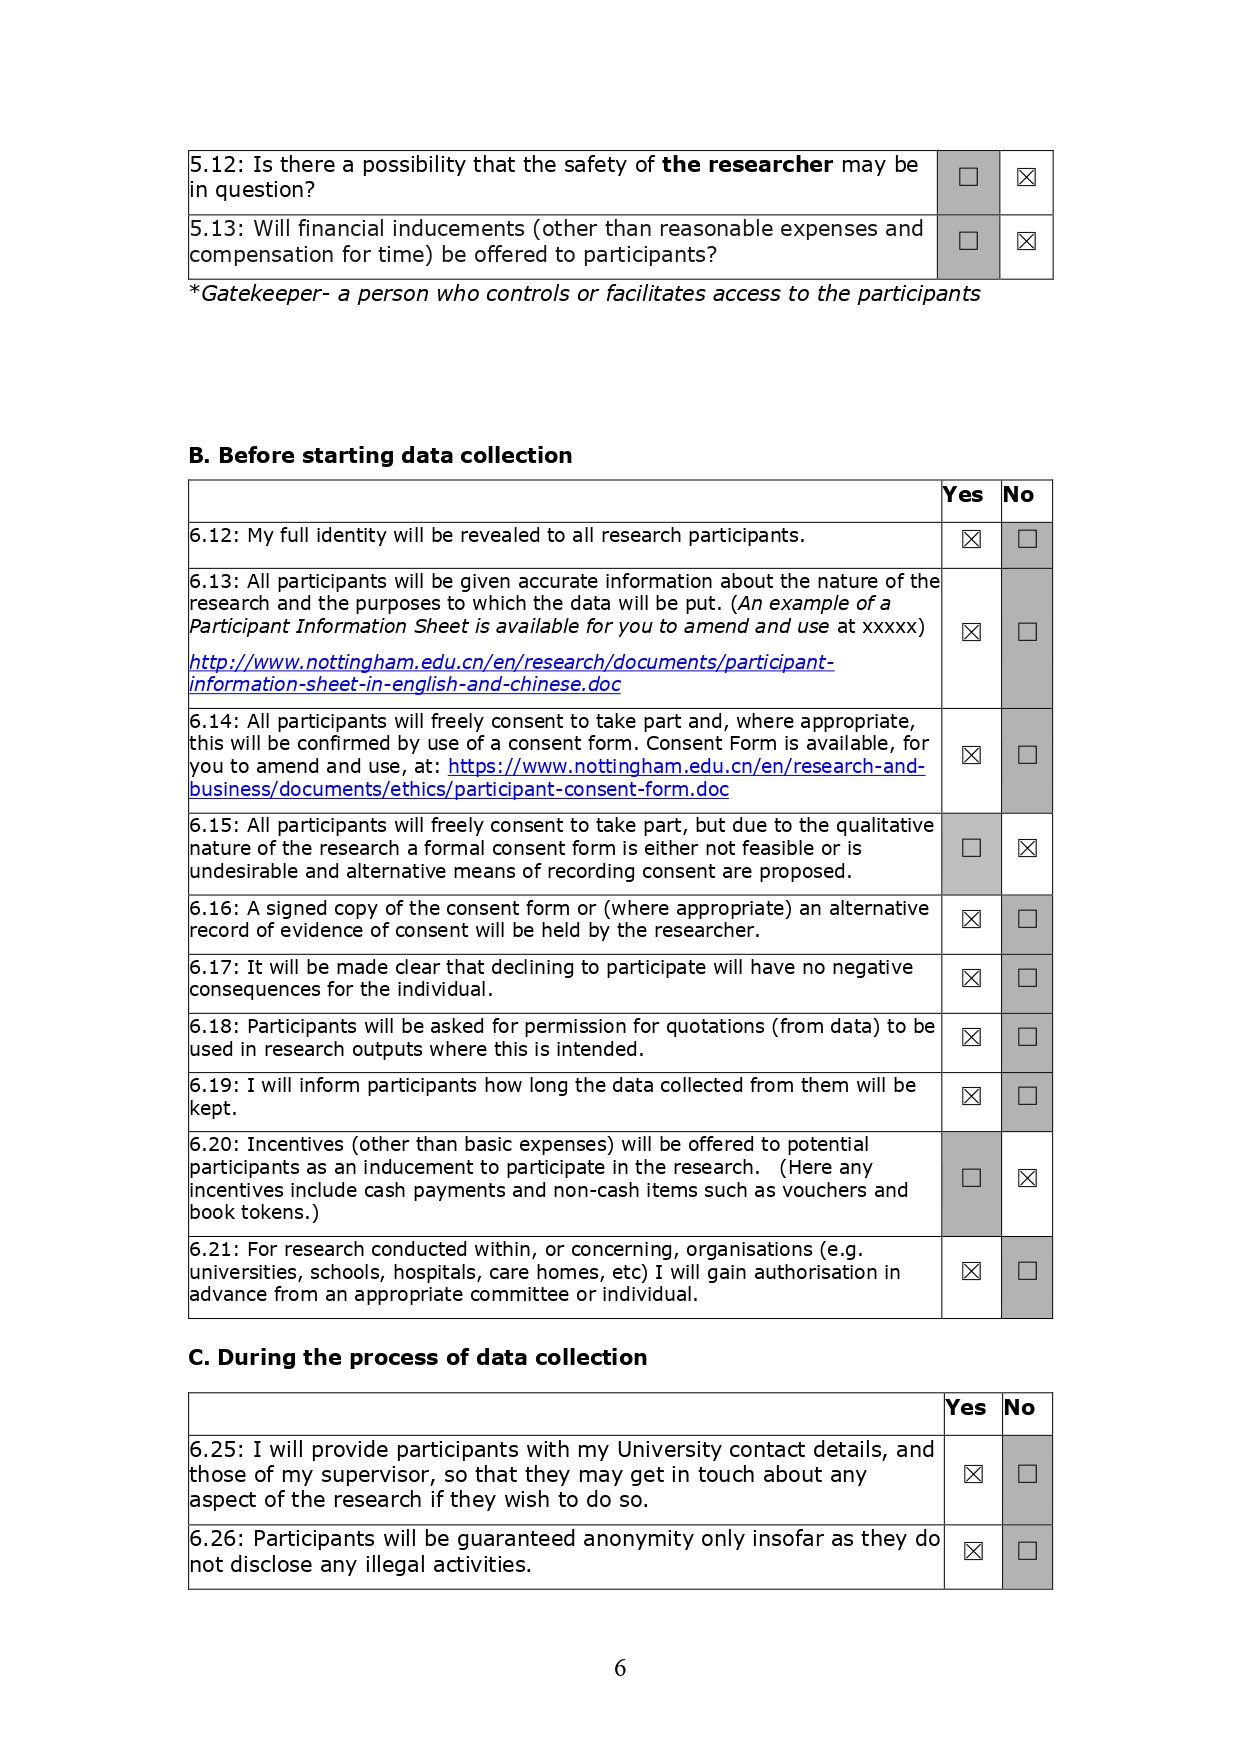
\includegraphics[width=1.0\textwidth]{images/appendix/ethics/Team.202513.FullChecklist_page-0006.jpg}
\end{figure}
\begin{figure}[H]
    \centering
    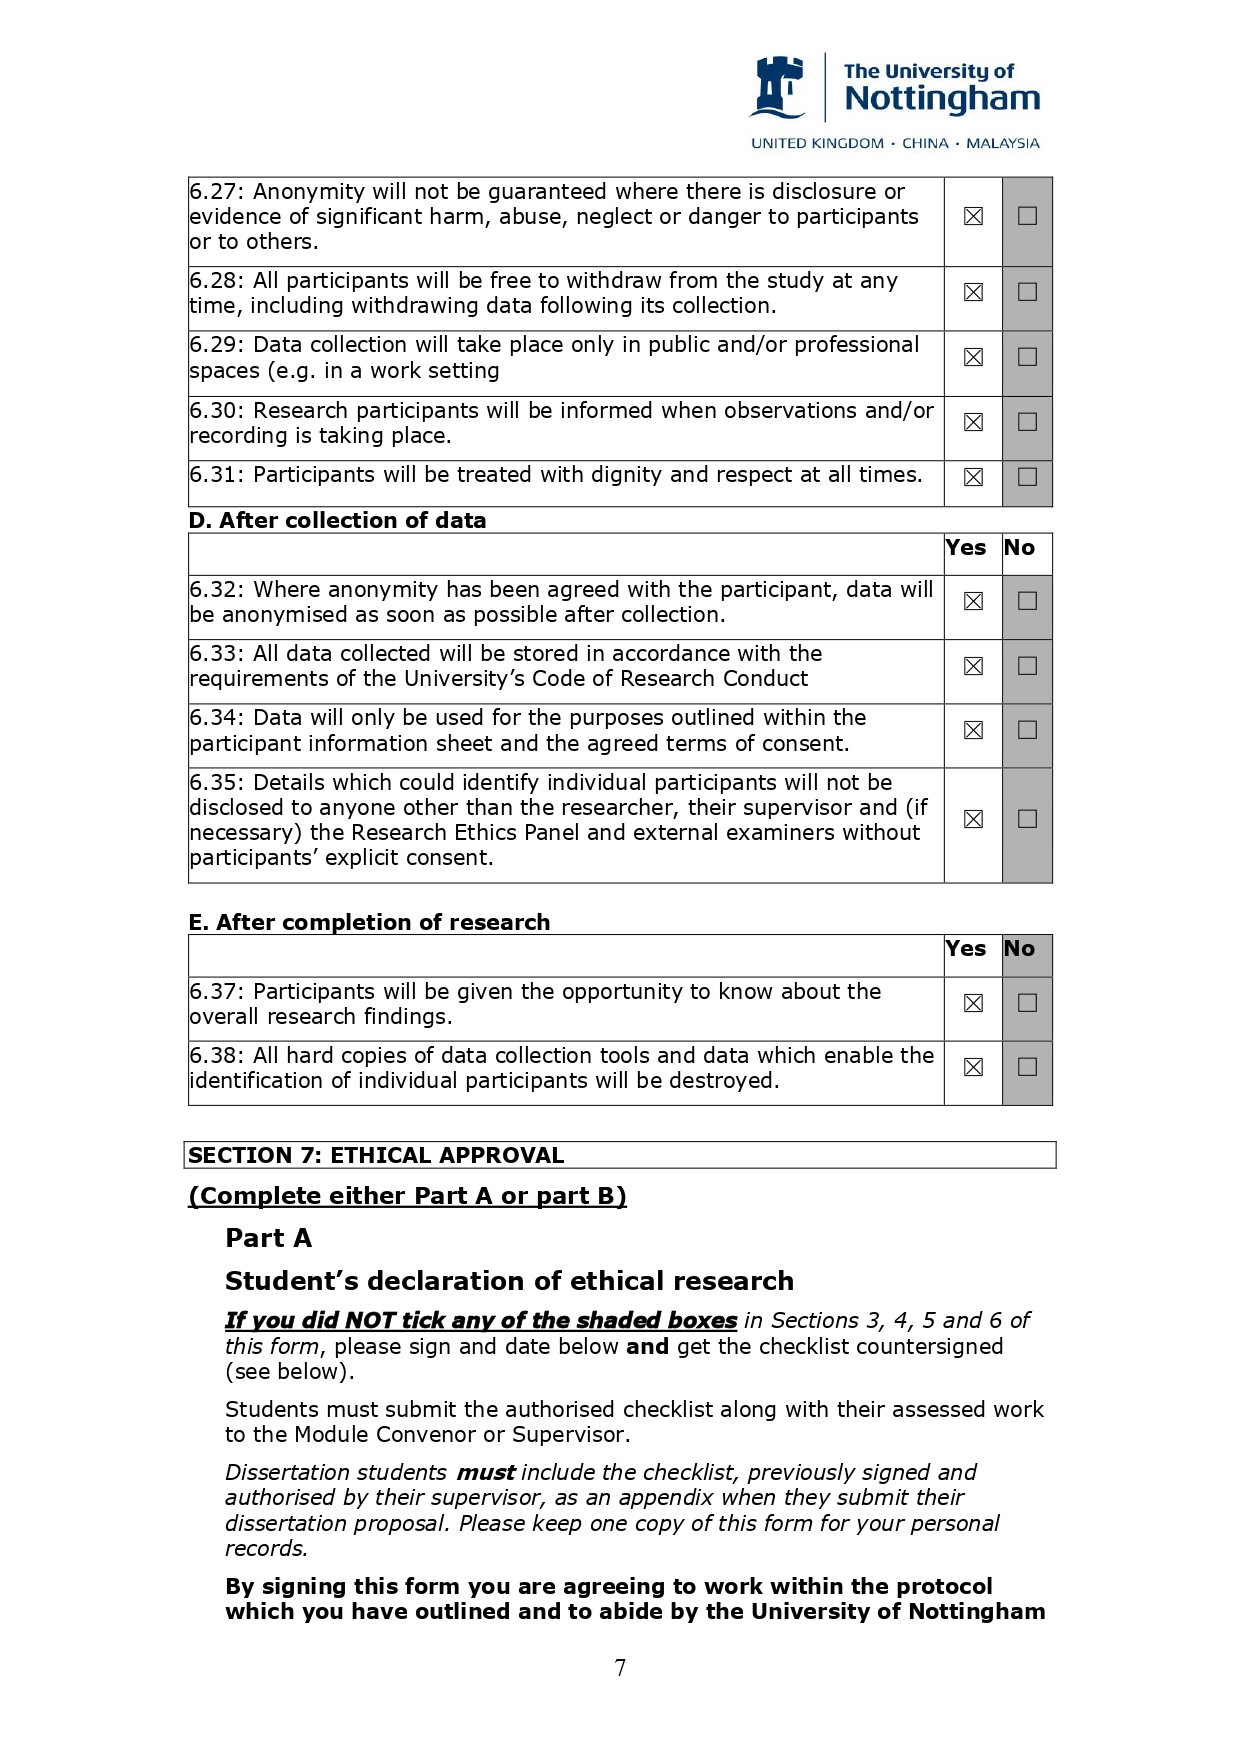
\includegraphics[width=1.0\textwidth]{images/appendix/ethics/Team.202513.FullChecklist_page-0007.jpg}
\end{figure}
\begin{figure}[H]
    \centering
    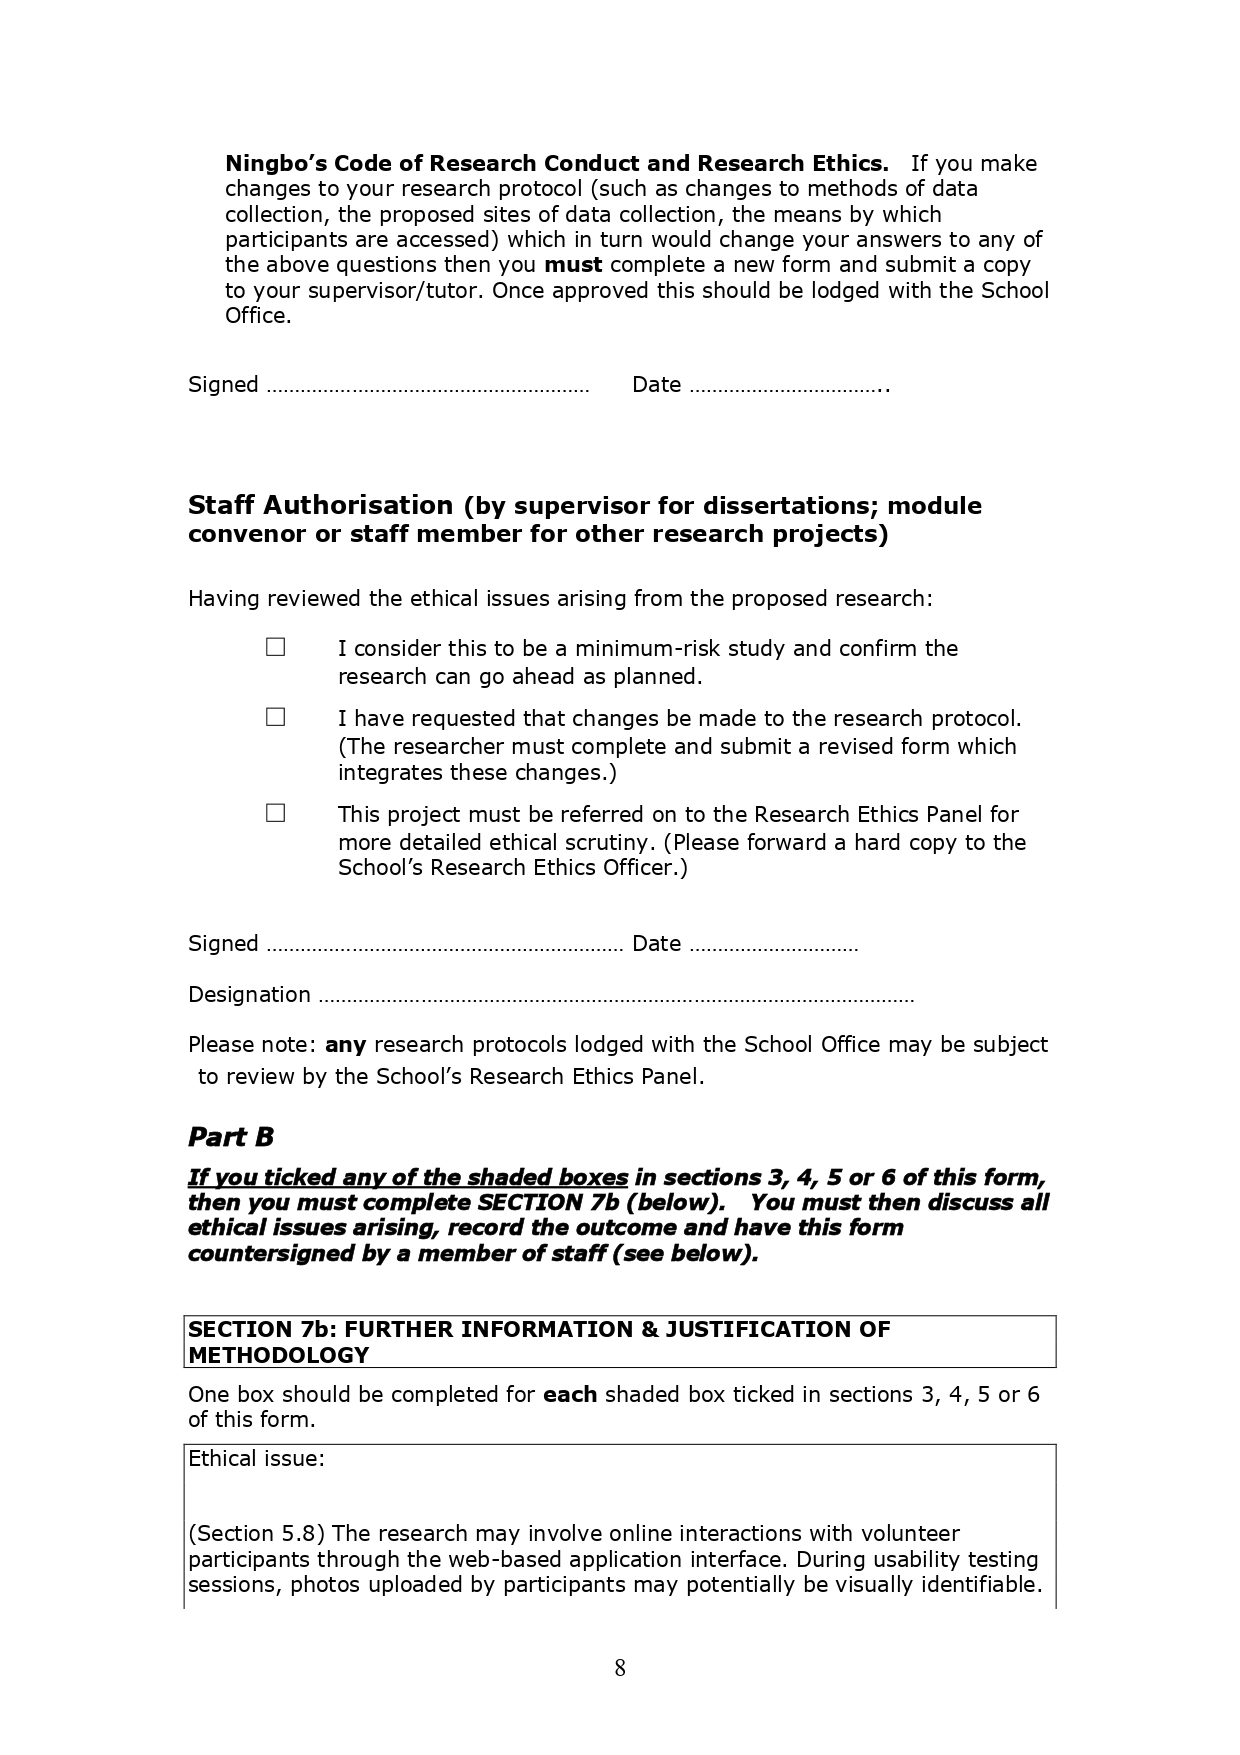
\includegraphics[width=1.0\textwidth]{images/appendix/ethics/Team.202513.FullChecklist_page-0008.jpg}
\end{figure}
\begin{figure}[H]
    \centering
    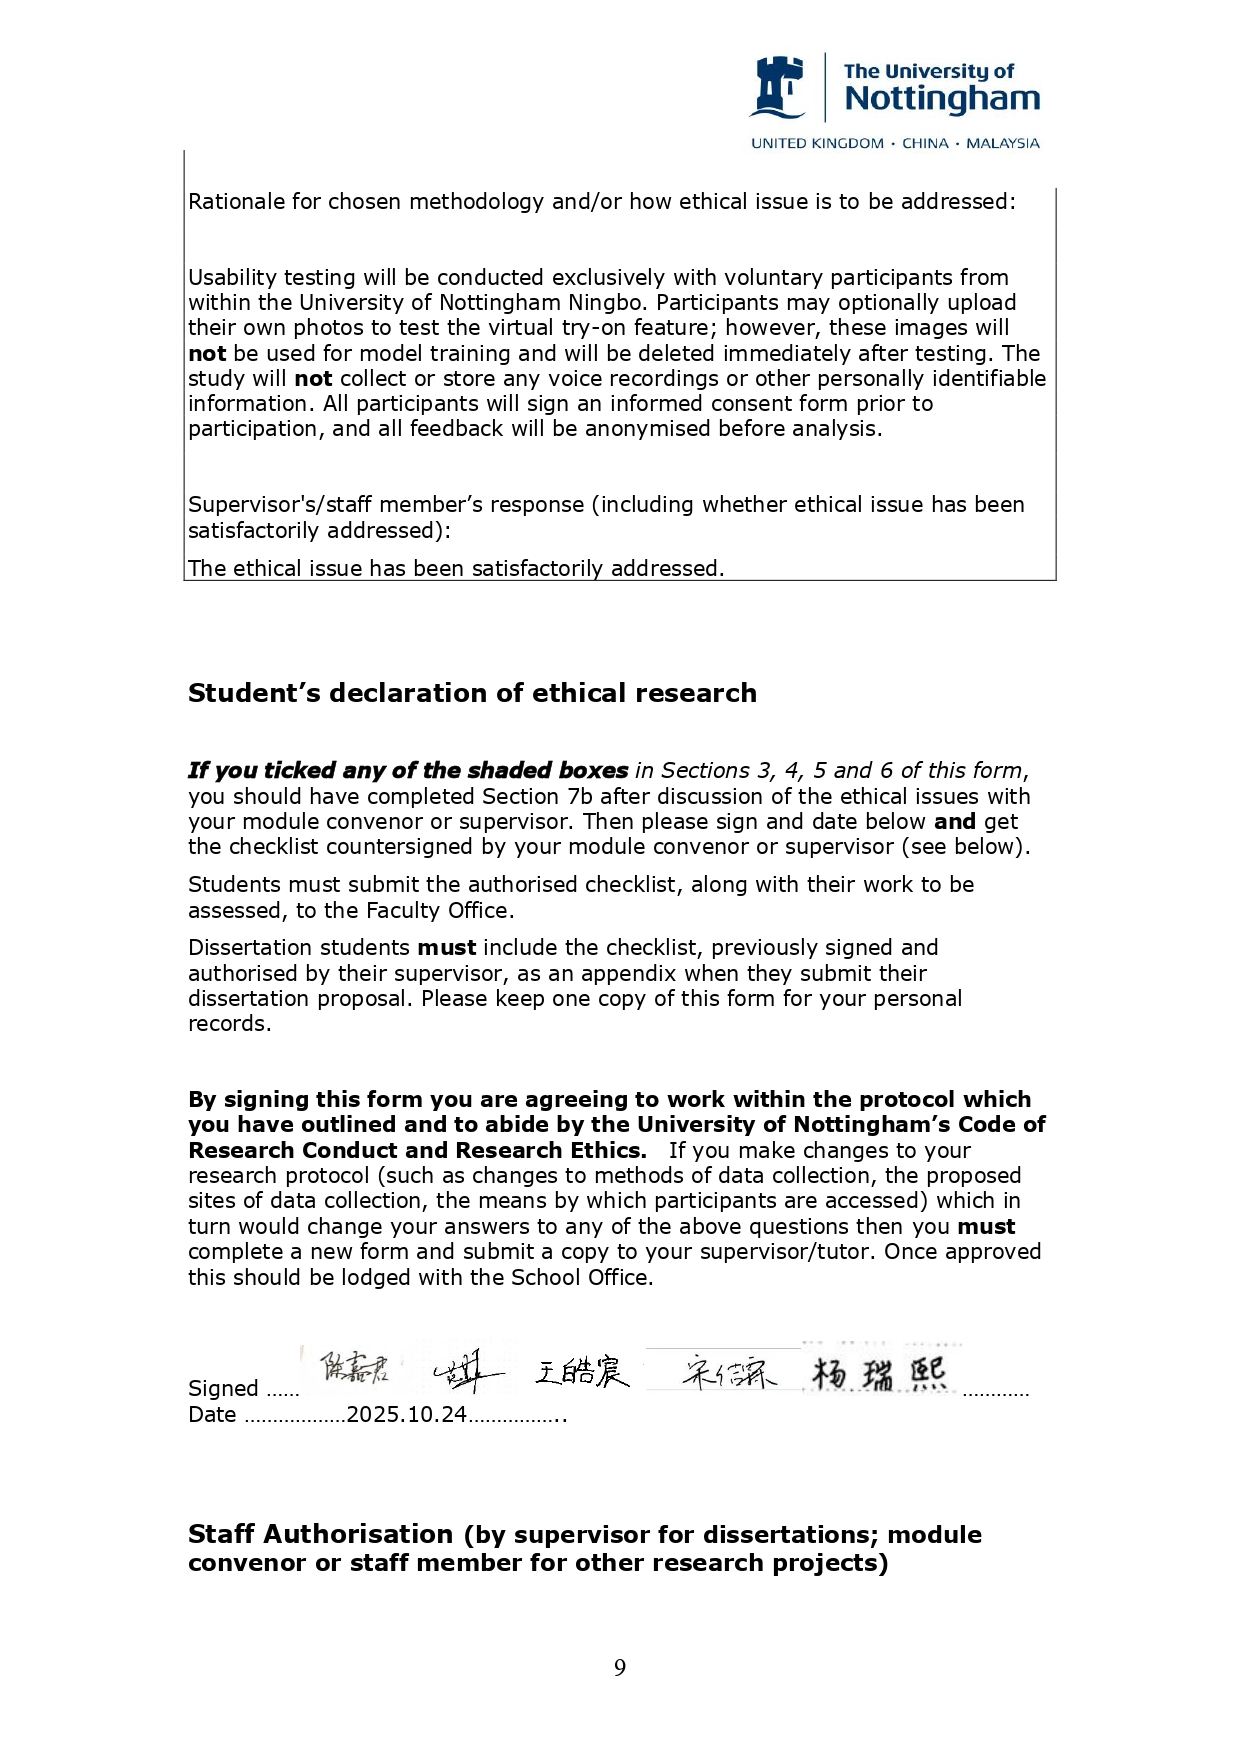
\includegraphics[width=1.0\textwidth]{images/appendix/ethics/Team.202513.FullChecklist_page-0009.jpg}
\end{figure}
\begin{figure}[H]
    \centering
    
\includegraphics[width=1.0\textwidth]{images/appendix/ethics/Team.202513.FullChecklist_page-0010.jpg}
\end{figure}



\chapter{Consent Form and Questionnaire}
\section{Participant Consent Form}
\begin{figure}[H]
    \centering
    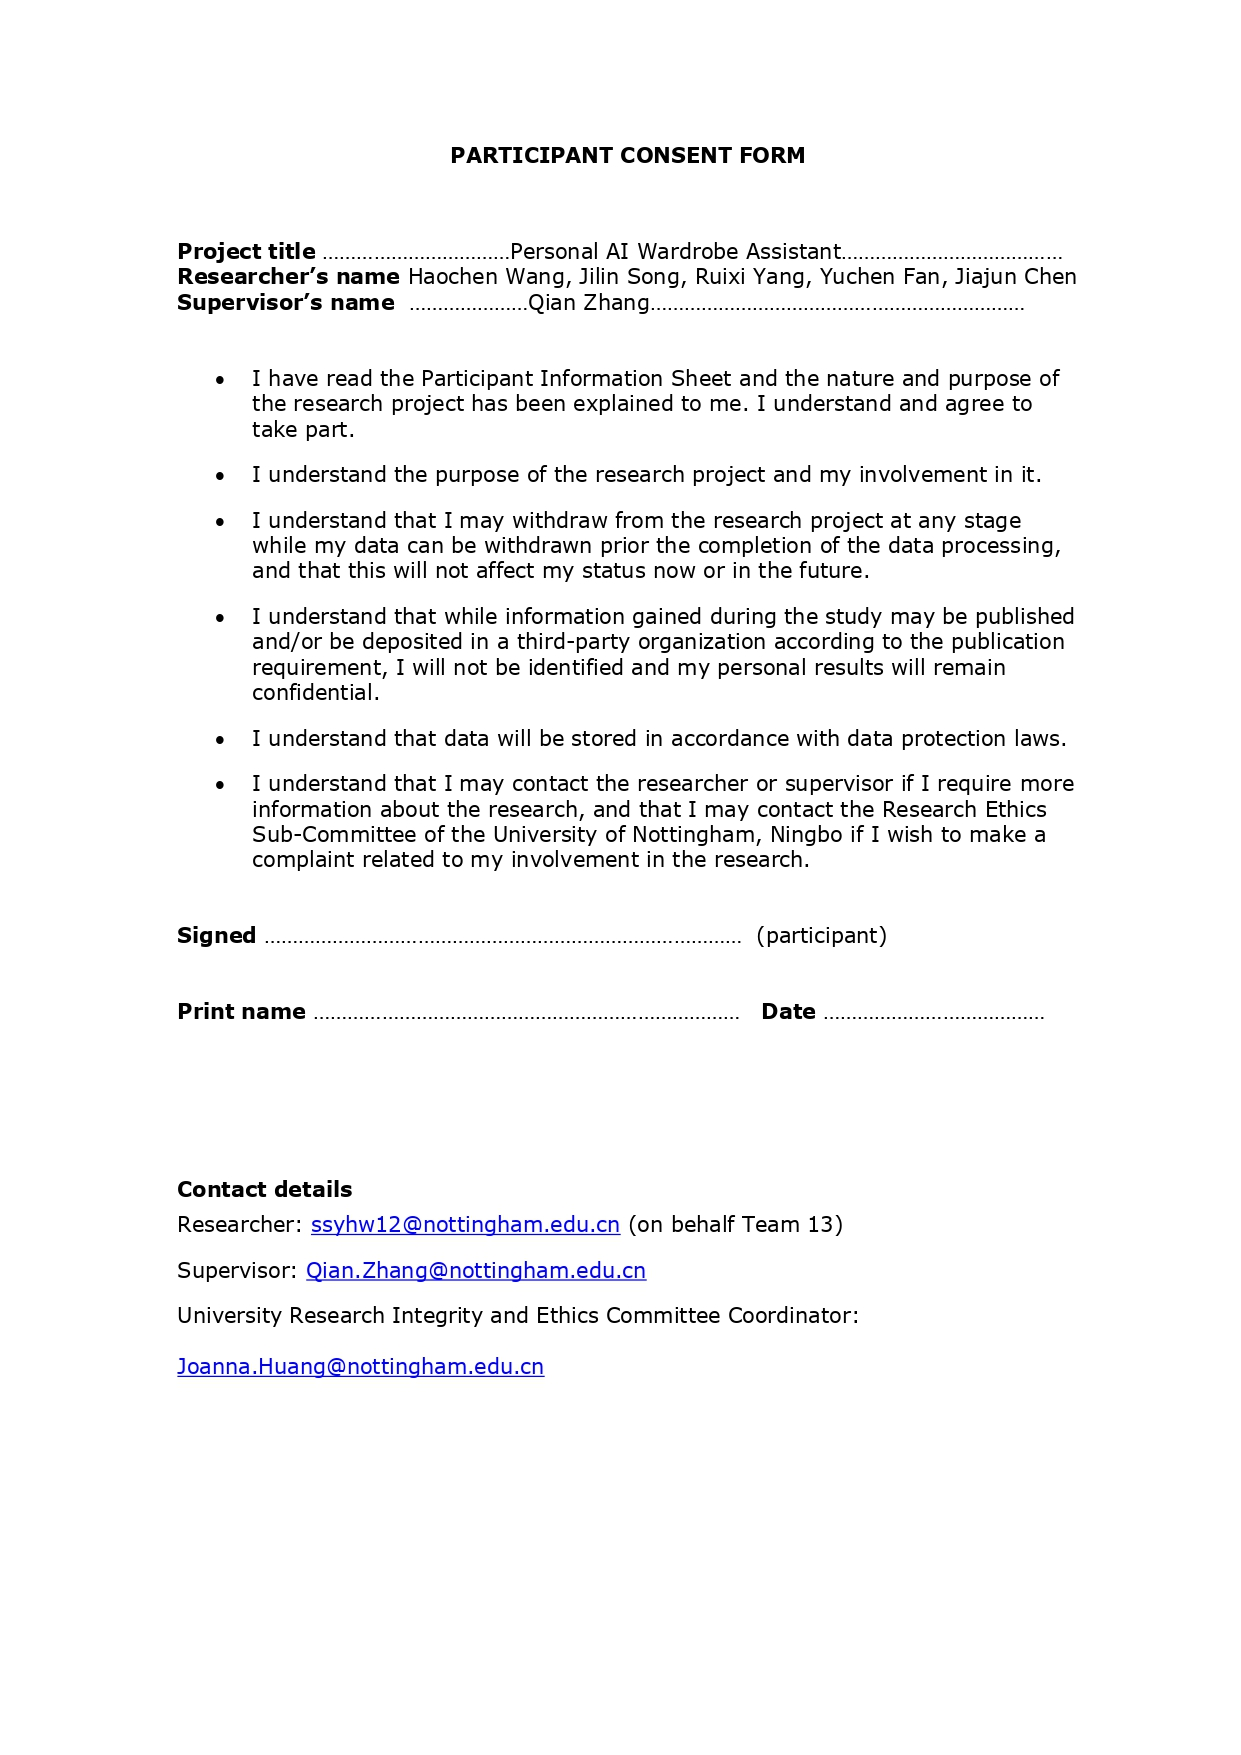
\includegraphics[width=1.0\textwidth]{images/appendix/questionnaire/Team.202513.Participant-Consent-Form_page-0001.jpg}
\end{figure}
\begin{figure}[H]
    \centering
    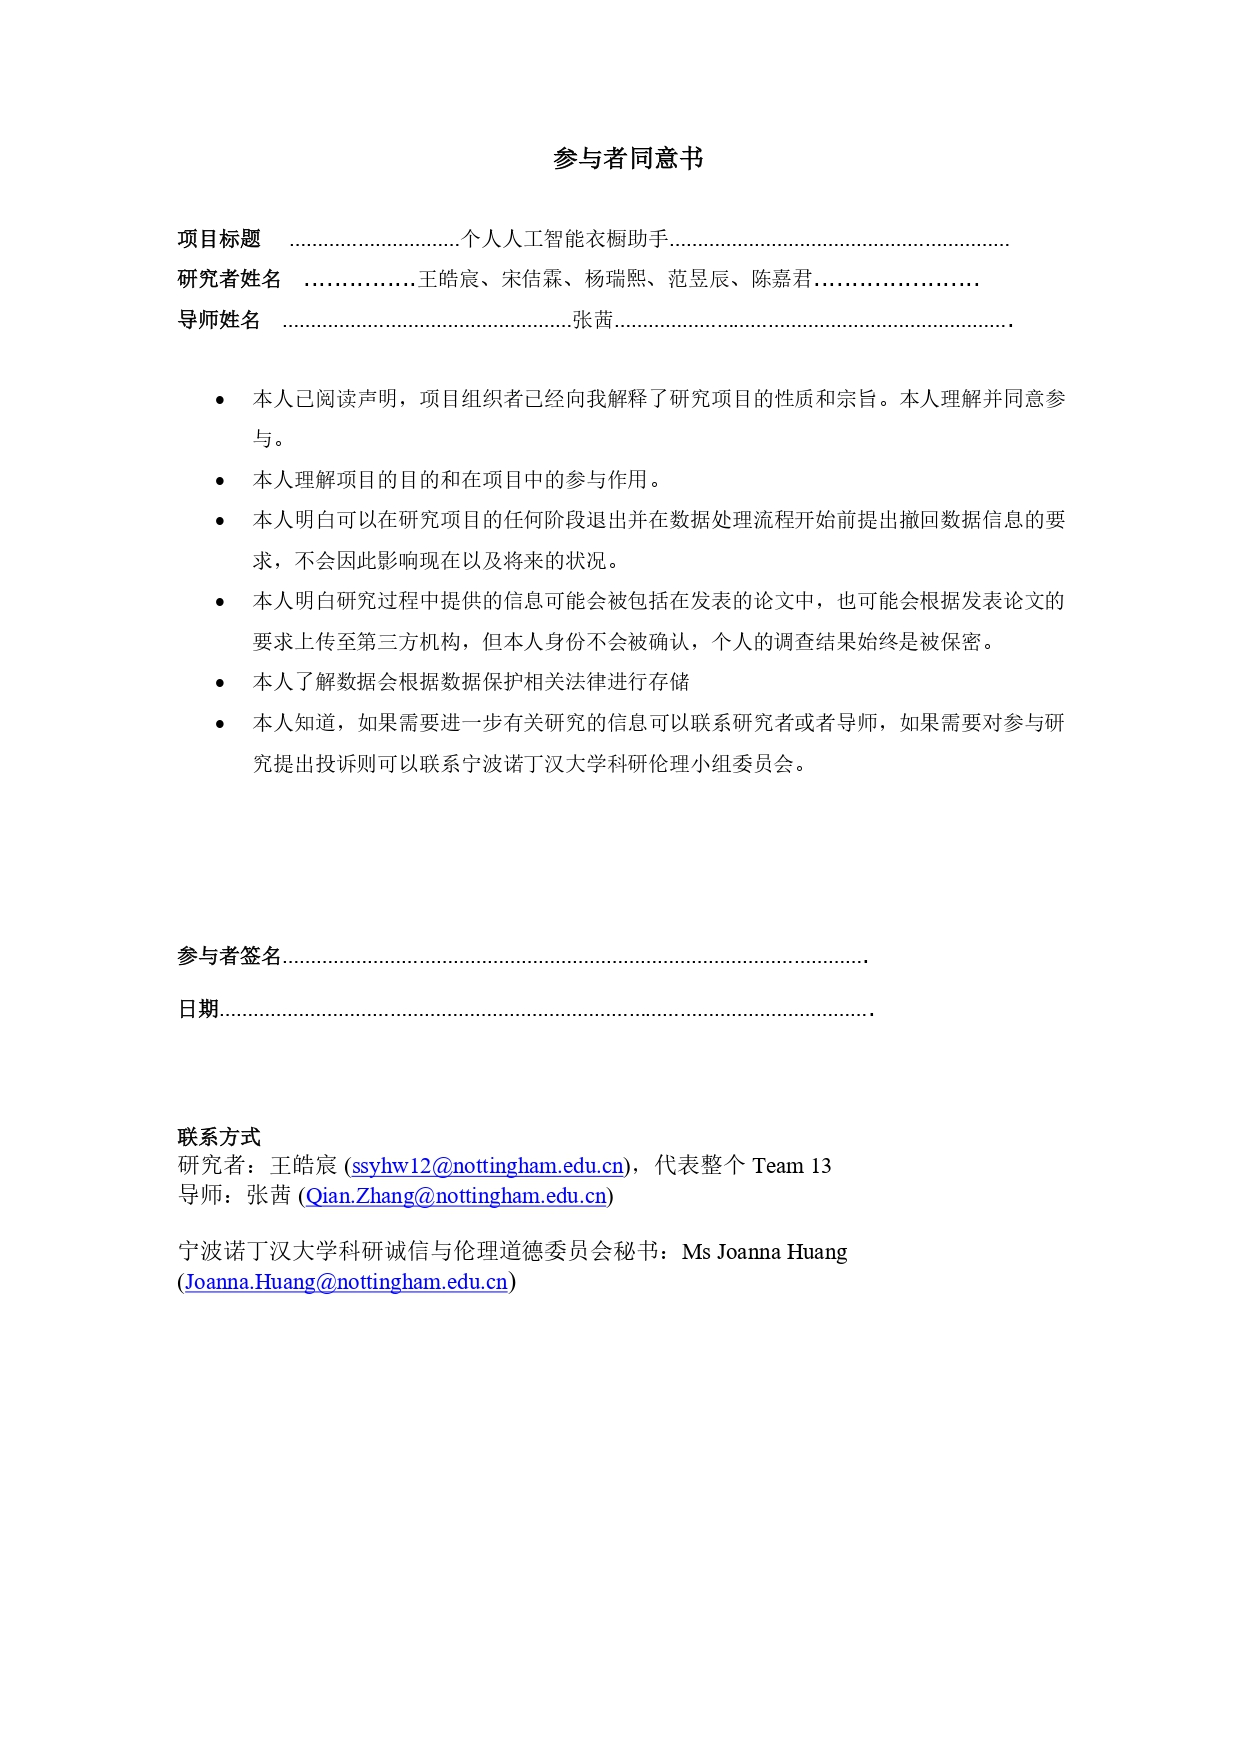
\includegraphics[width=1.0\textwidth]{images/appendix/questionnaire/Team.202513.Participant-Consent-Form_page-0002.jpg}
\end{figure}

\section{Participant Information Sheet}
\begin{figure}[H]
    \centering
    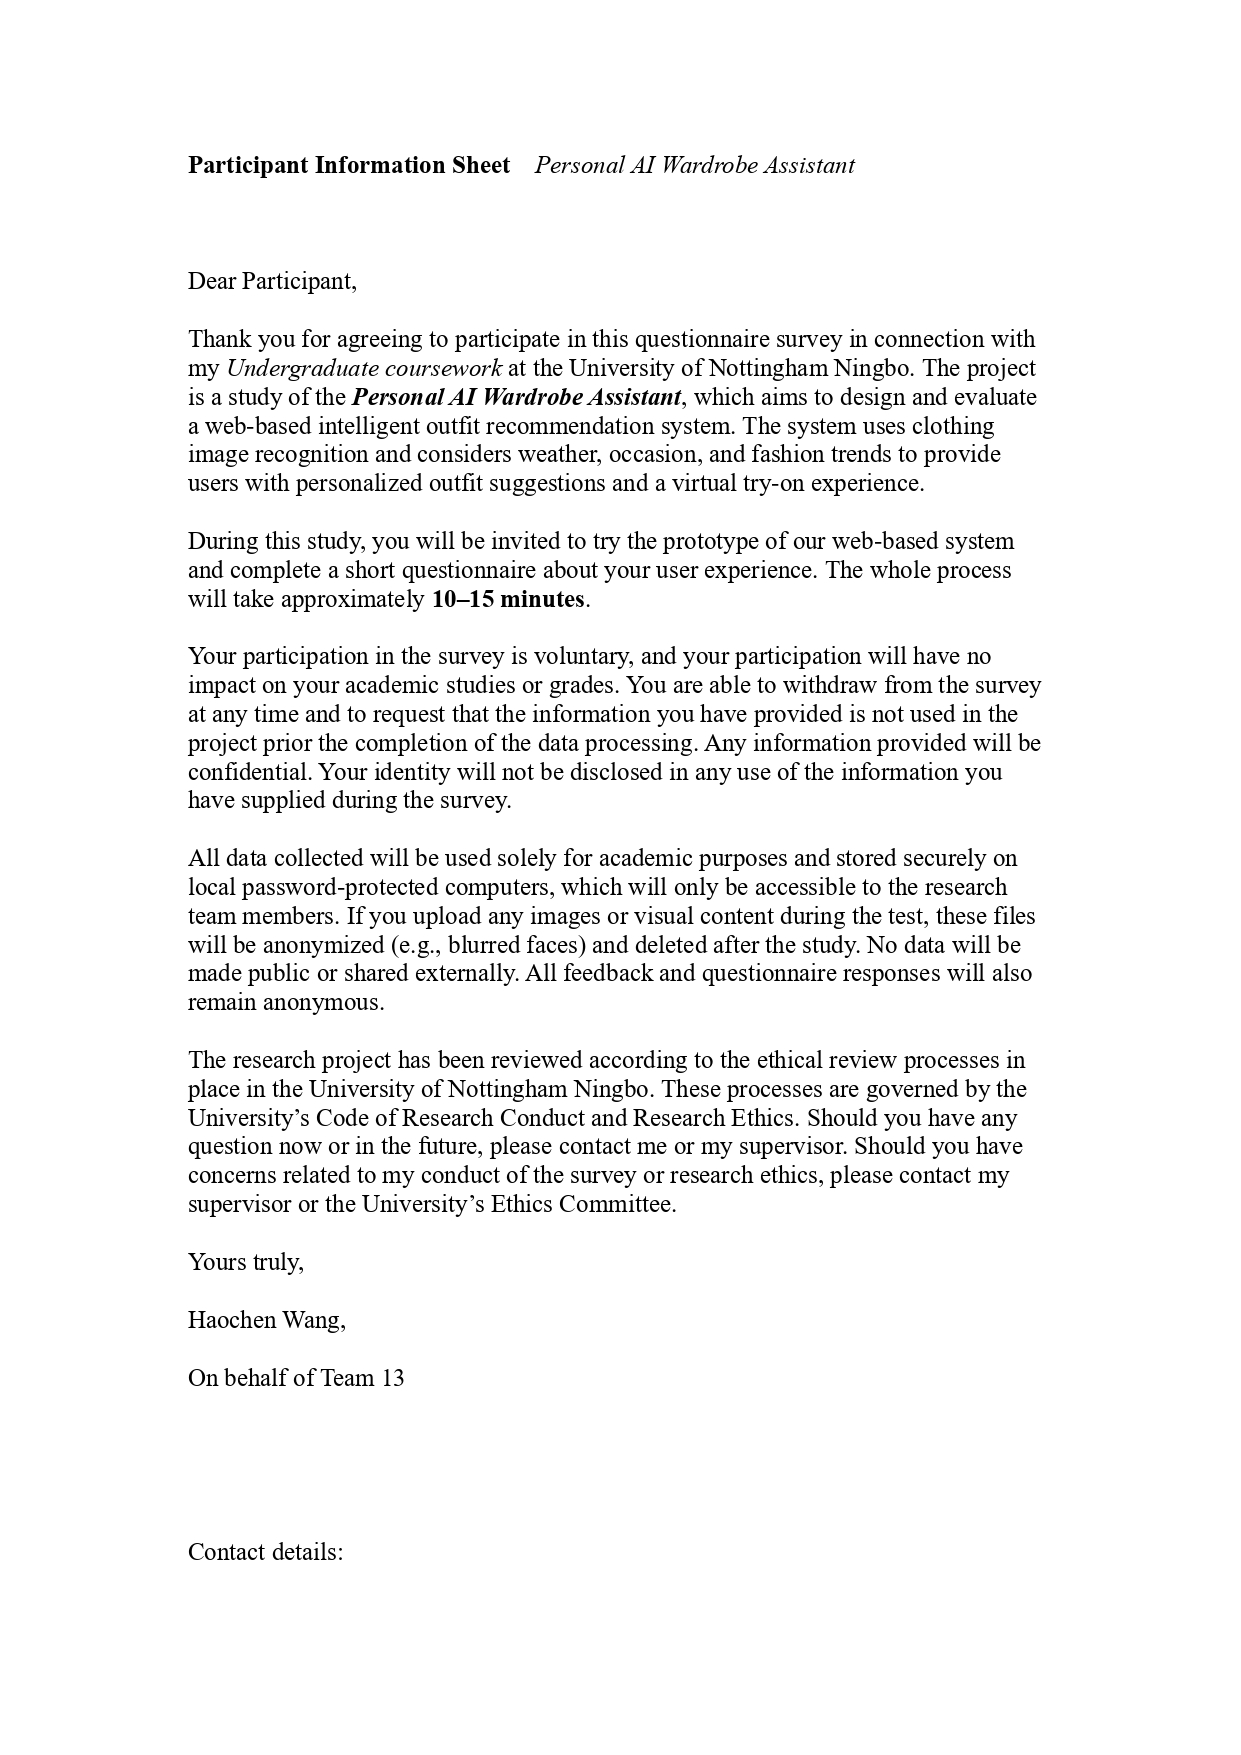
\includegraphics[width=1.0\textwidth]{images/appendix/questionnaire/Team202513.Participant-Information-Sheet_page-0001.jpg}
\end{figure}
\begin{figure}[H]
    \centering
    
\includegraphics[width=1.0\textwidth]{images/appendix/questionnaire/Team202513.Participant-Information-Sheet_page-0002.jpg}
\end{figure}
\begin{figure}[H]
    \centering
    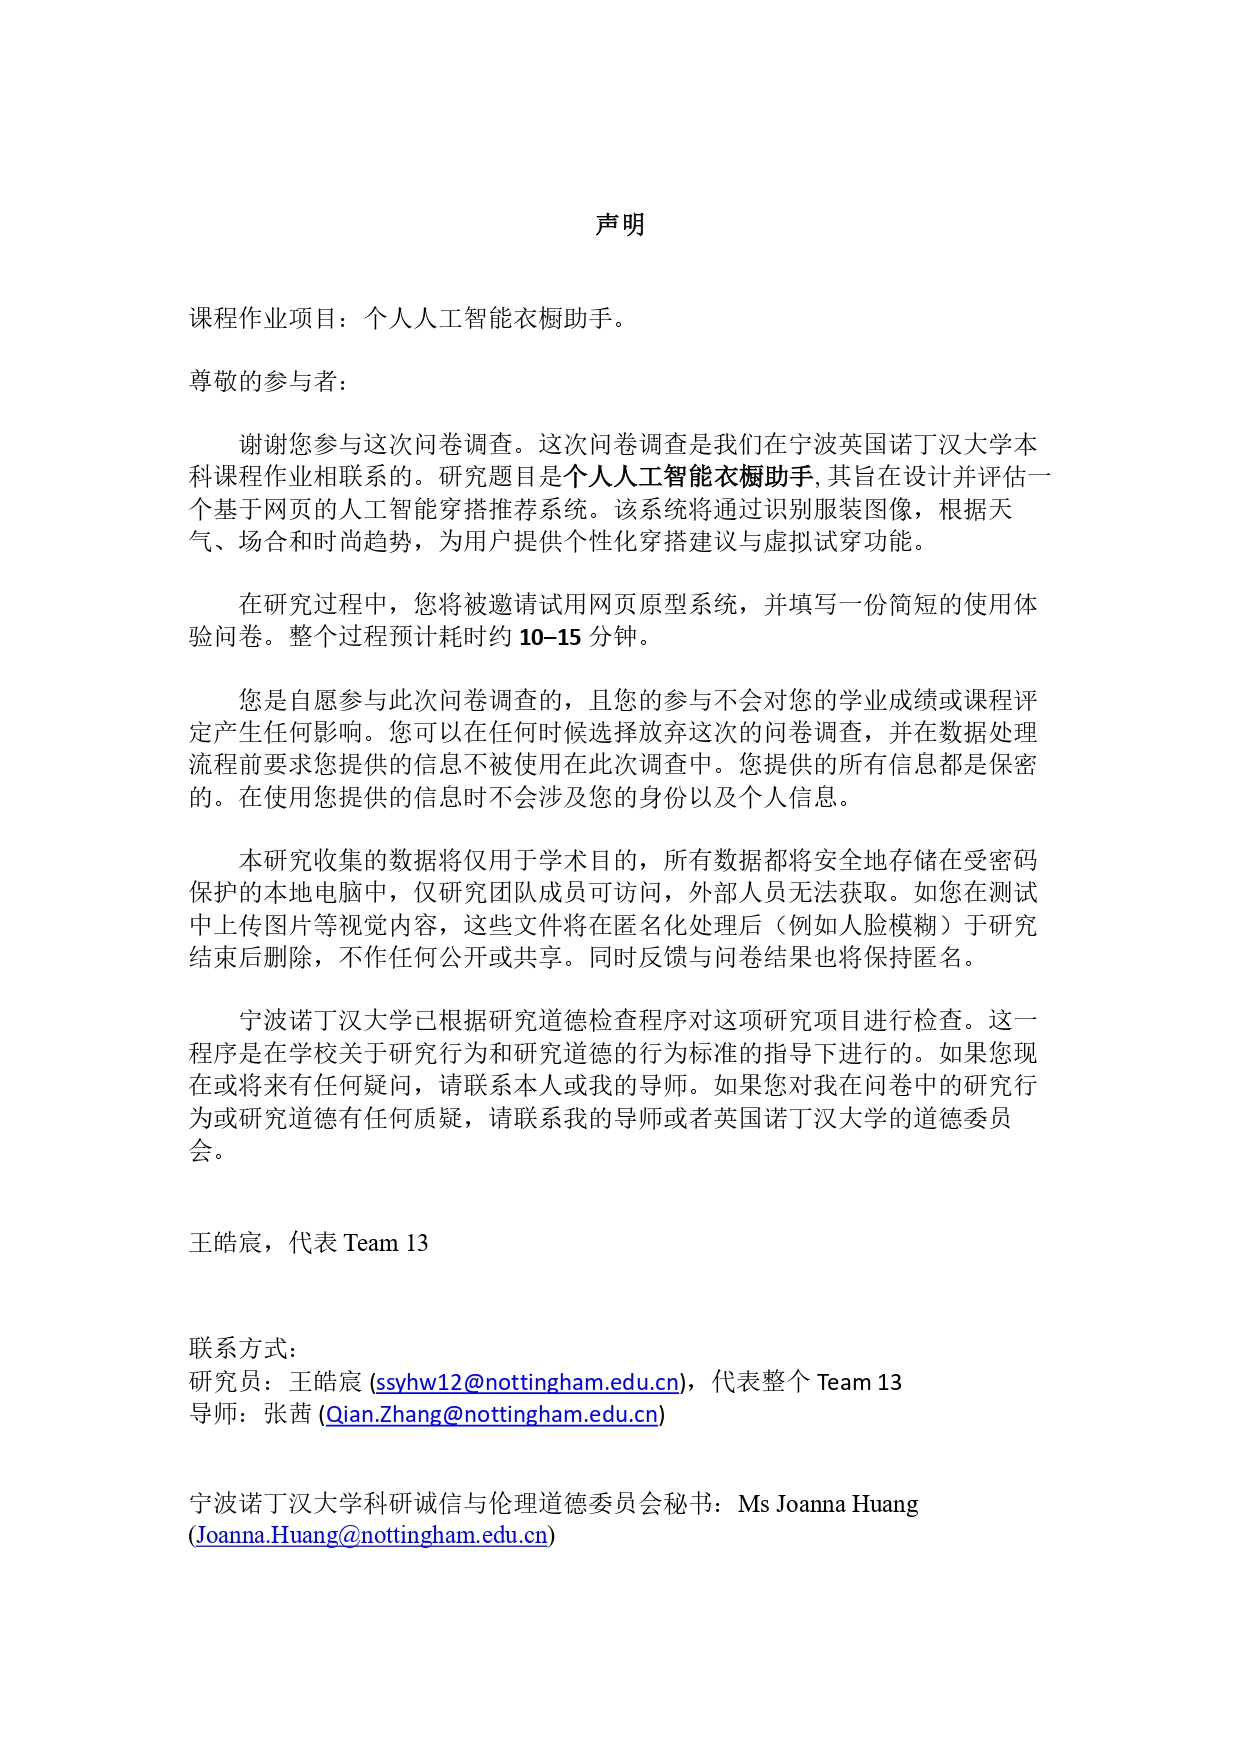
\includegraphics[width=1.0\textwidth]{images/appendix/questionnaire/Team202513.Participant-Information-Sheet_page-0003.jpg}
\end{figure}

\section{Questionnaire}
\label{questionnaire}
\begin{figure}[H]
    \centering
    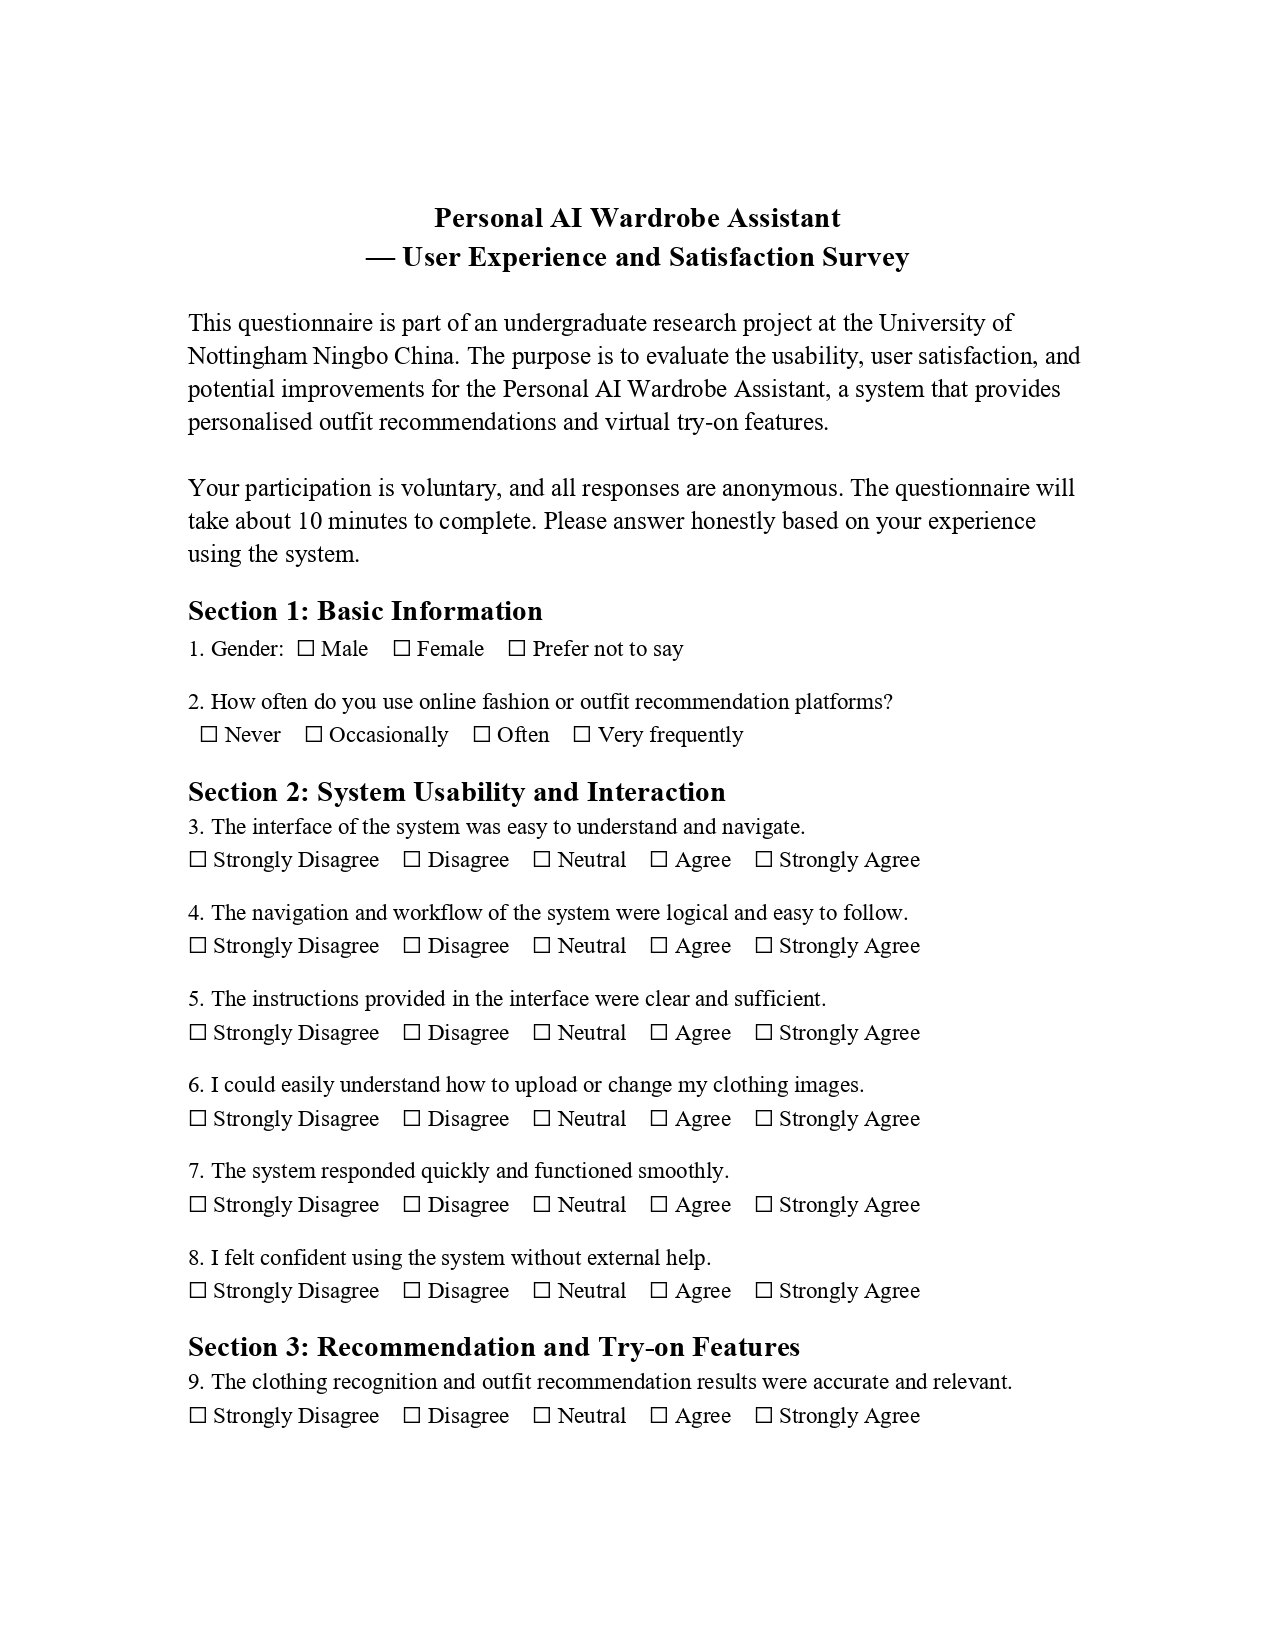
\includegraphics[width=1.25\textwidth]{images/appendix/questionnaire/Questionnaire_page-0001.jpg}
\end{figure}
\begin{figure}[H]
    \centering
    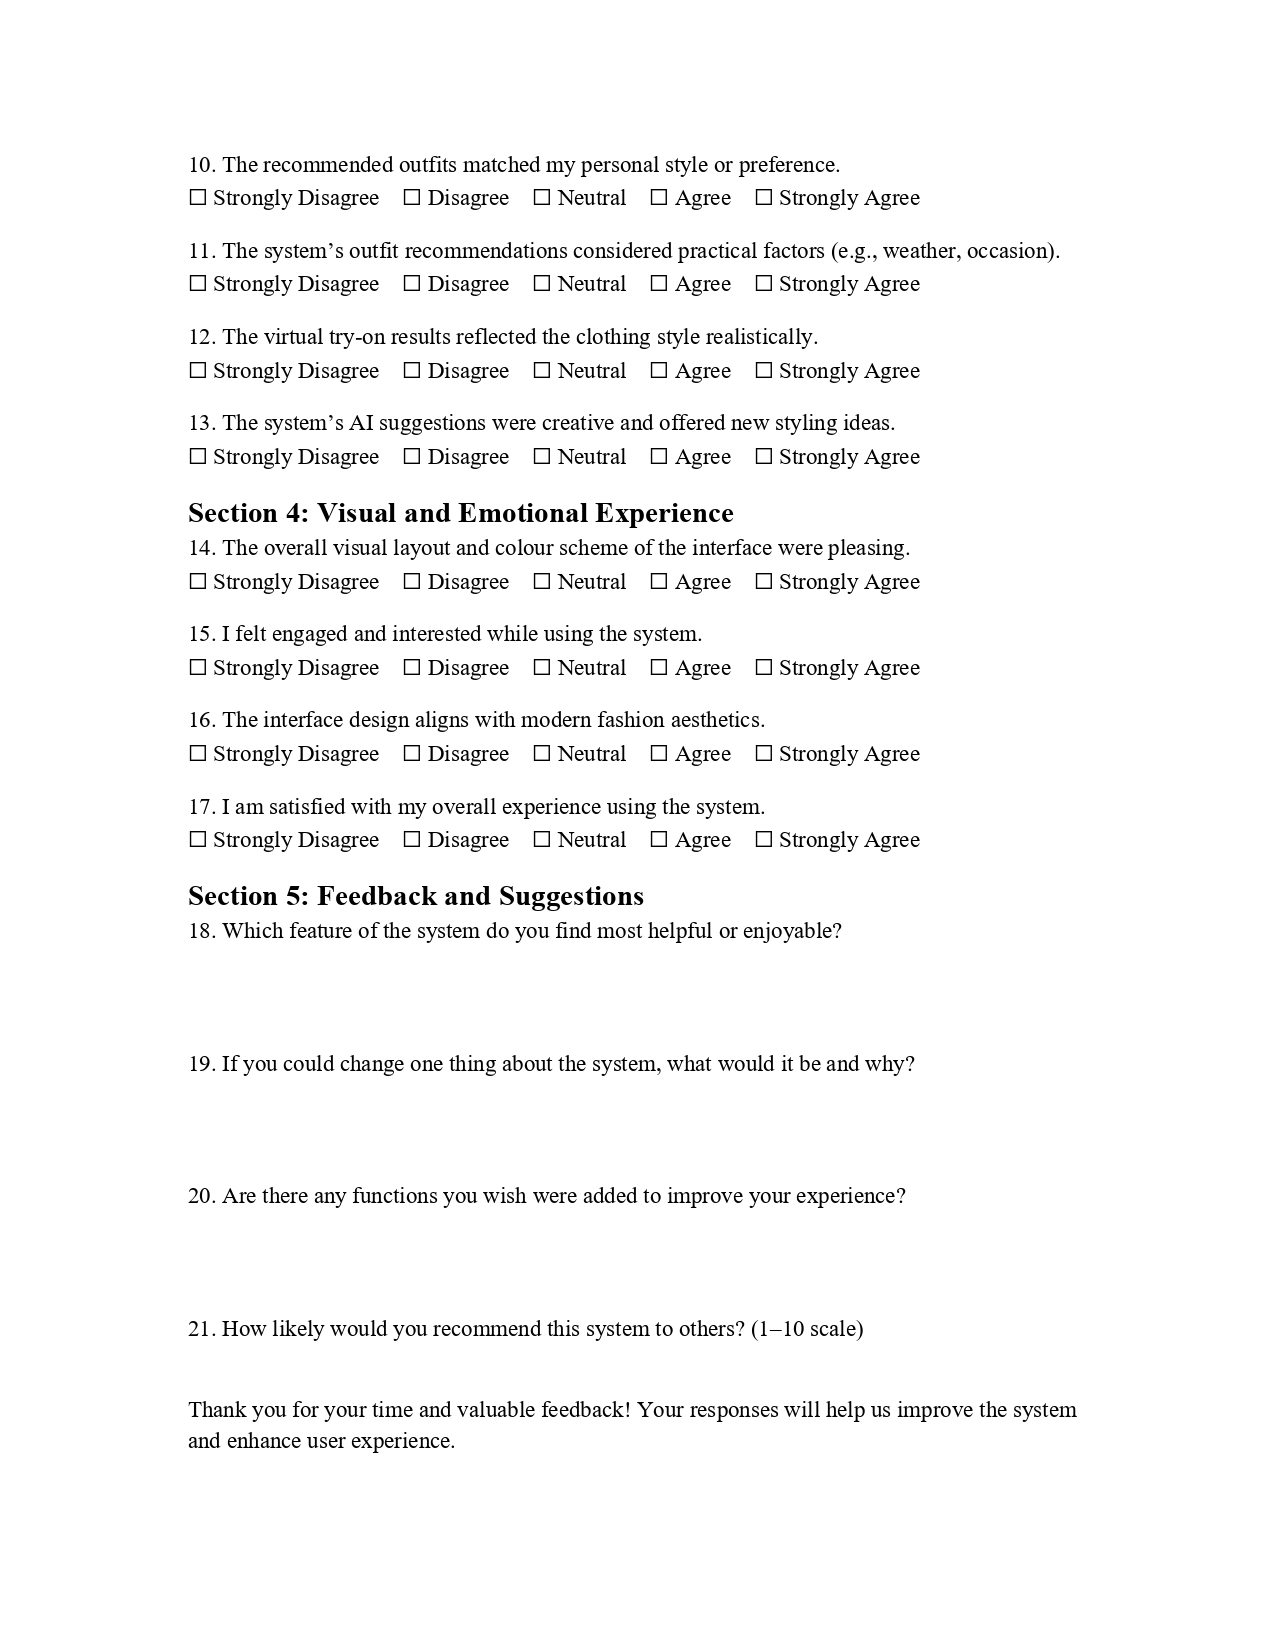
\includegraphics[width=1.25\textwidth]{images/appendix/questionnaire/Questionnaire_page-0002.jpg}
\end{figure}
\begin{figure}[H]
    \centering
    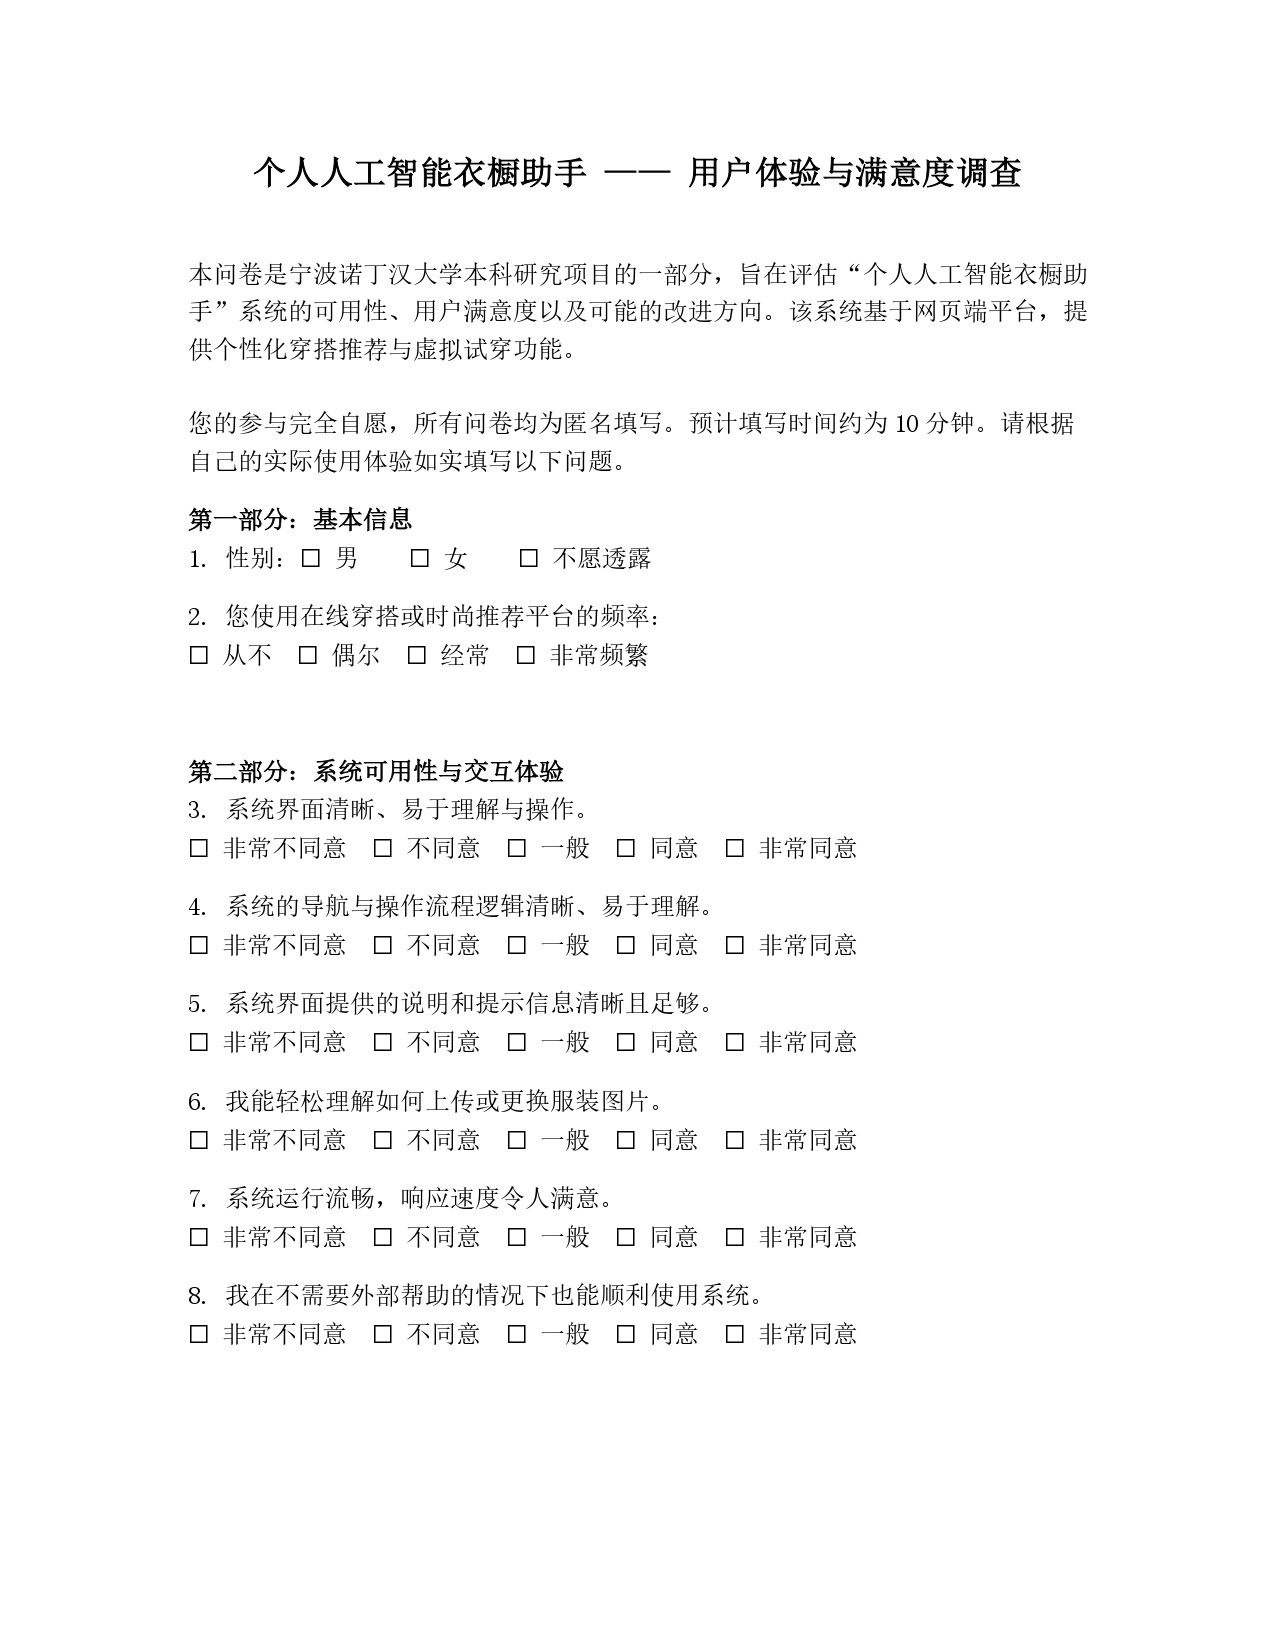
\includegraphics[width=1.2\textwidth]{images/appendix/questionnaire/Questionnaire_page-0003.jpg}
\end{figure}
\begin{figure}[H]
    \centering
    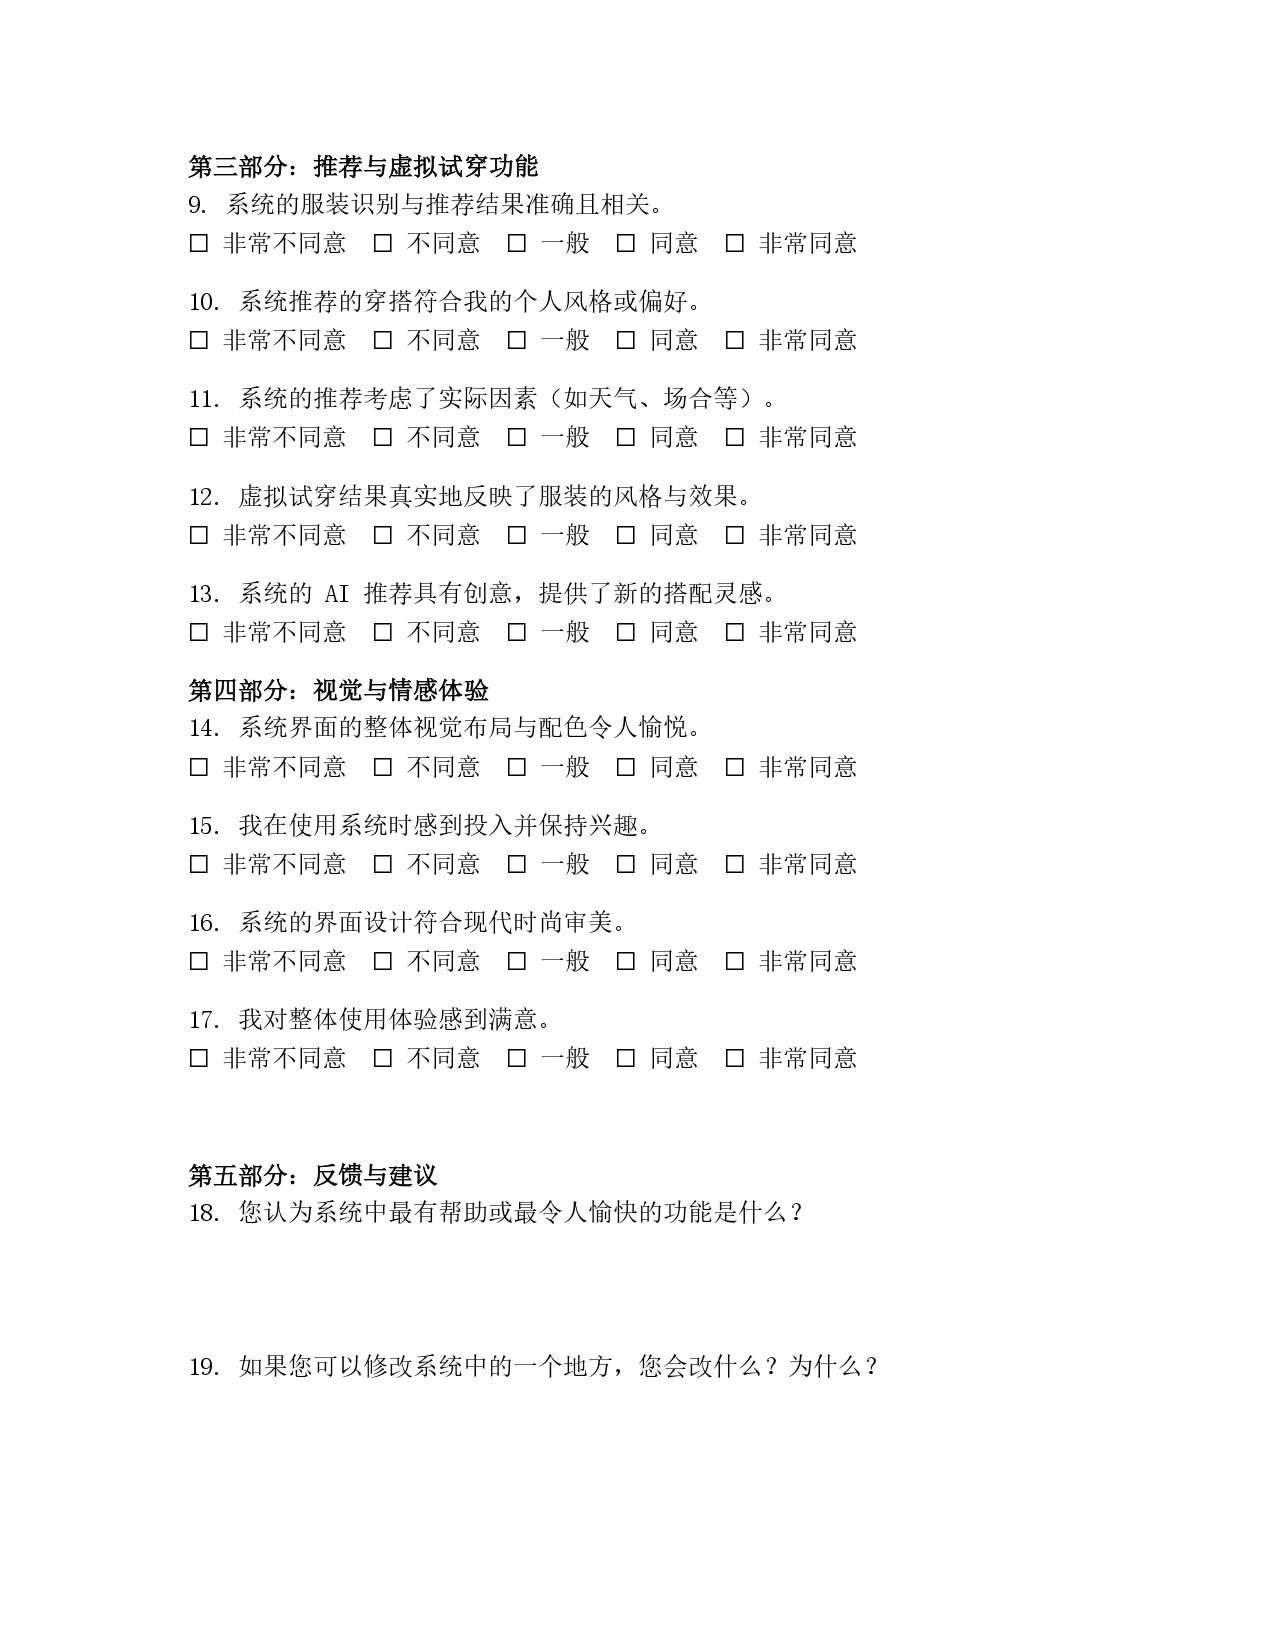
\includegraphics[width=1.25\textwidth]{images/appendix/questionnaire/Questionnaire_page-0004.jpg}
\end{figure}
\begin{figure}[H]
    \centering
    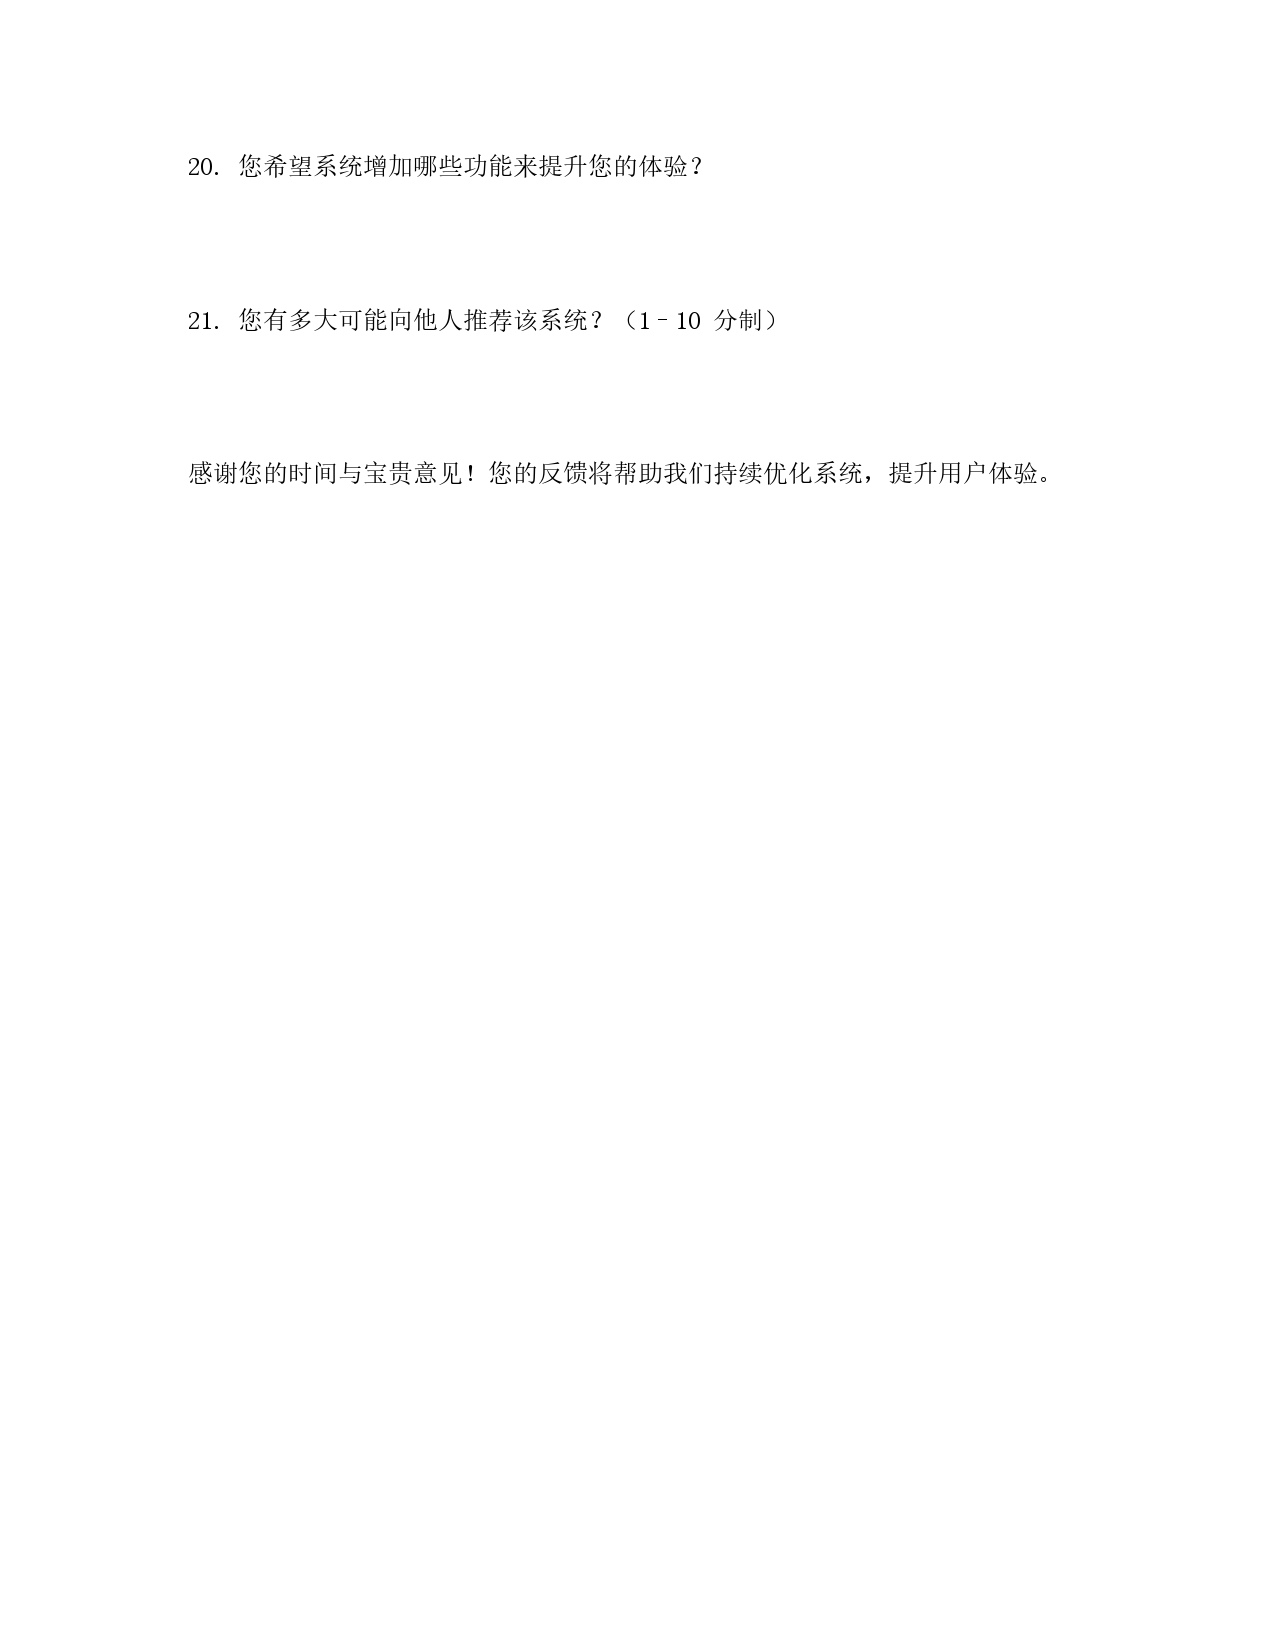
\includegraphics[width=1.25\textwidth]{images/appendix/questionnaire/Questionnaire_page-0005.jpg}
\end{figure}

\chapter{Installation Instructions}
\label{appendix:installation}
\begin{figure}[H]
    \centering
    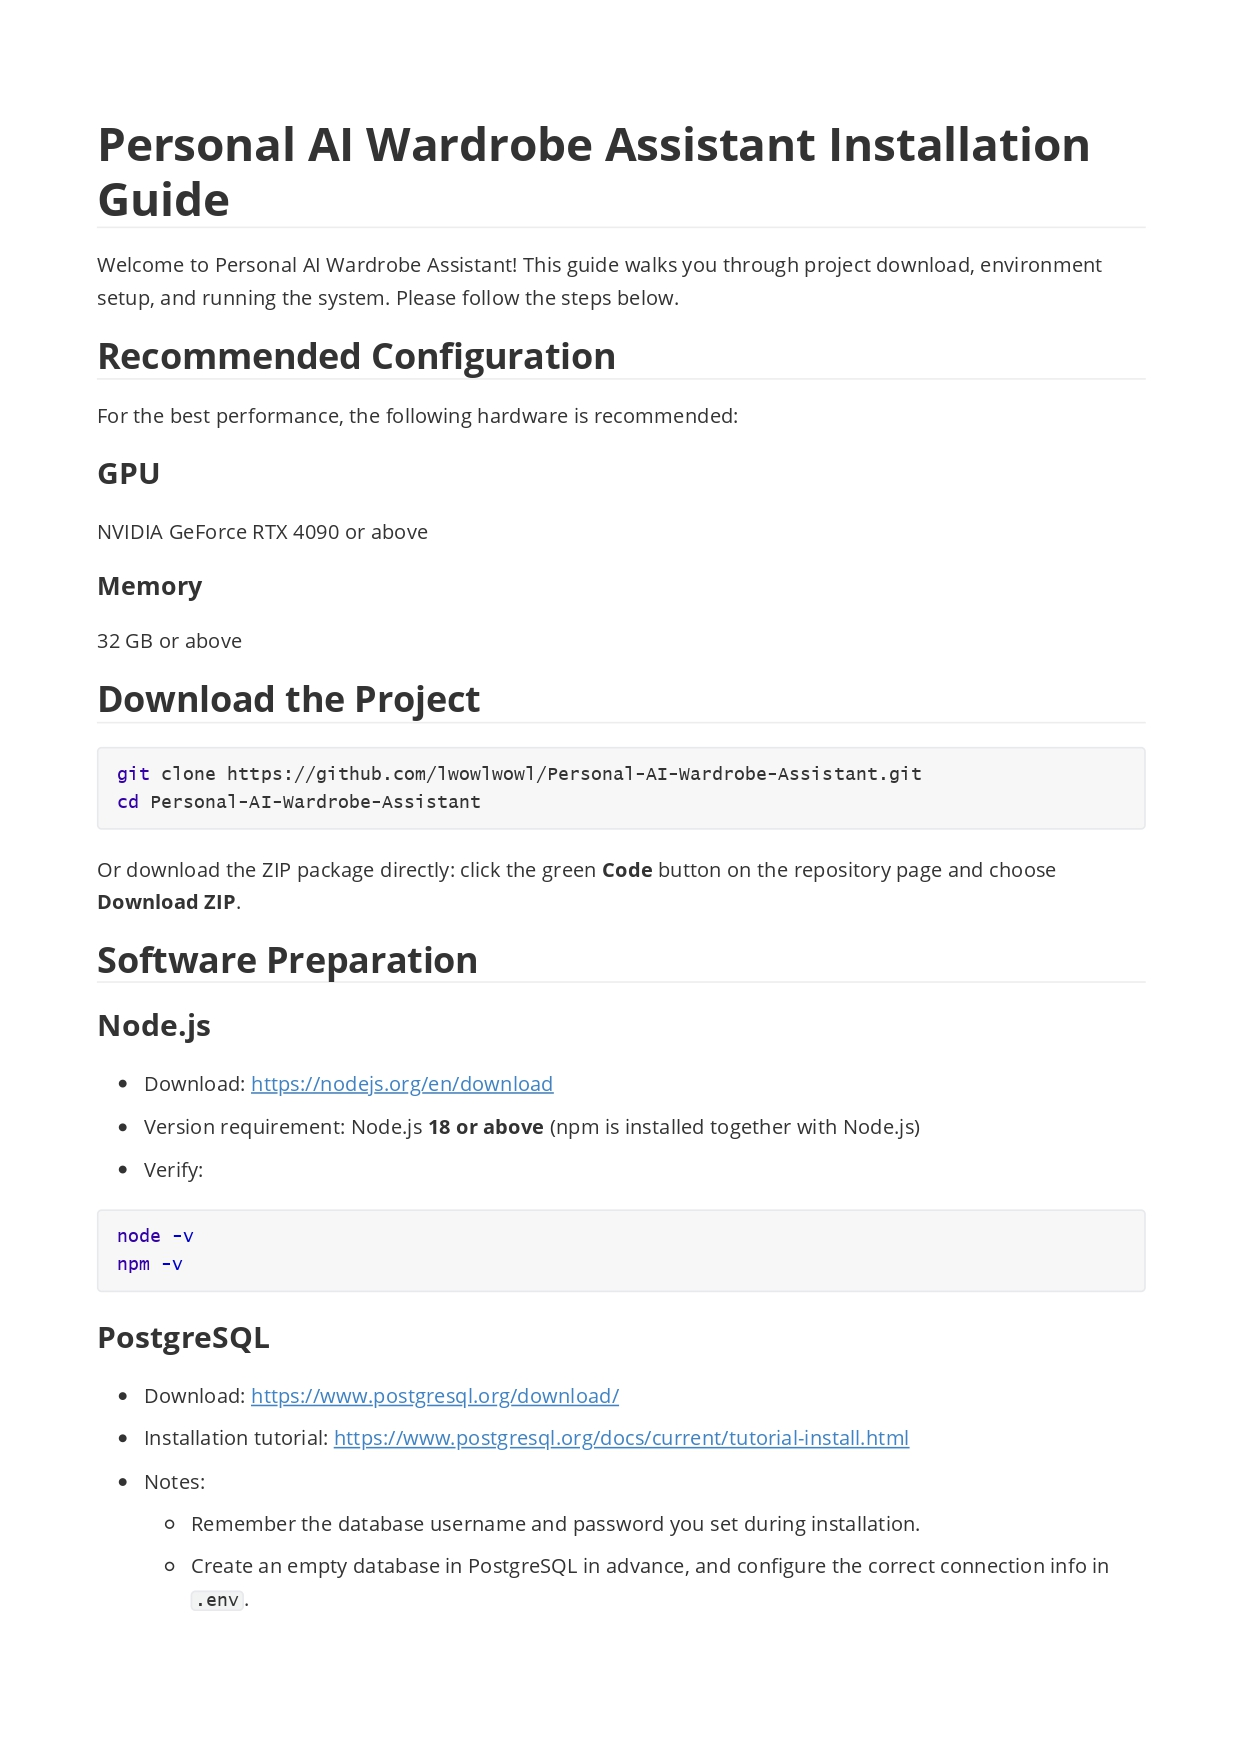
\includegraphics[width=0.95\textwidth]{images/appendix/install/installation_instruction_page-0001.jpg}
\end{figure}
\begin{figure}[H]
    \centering
    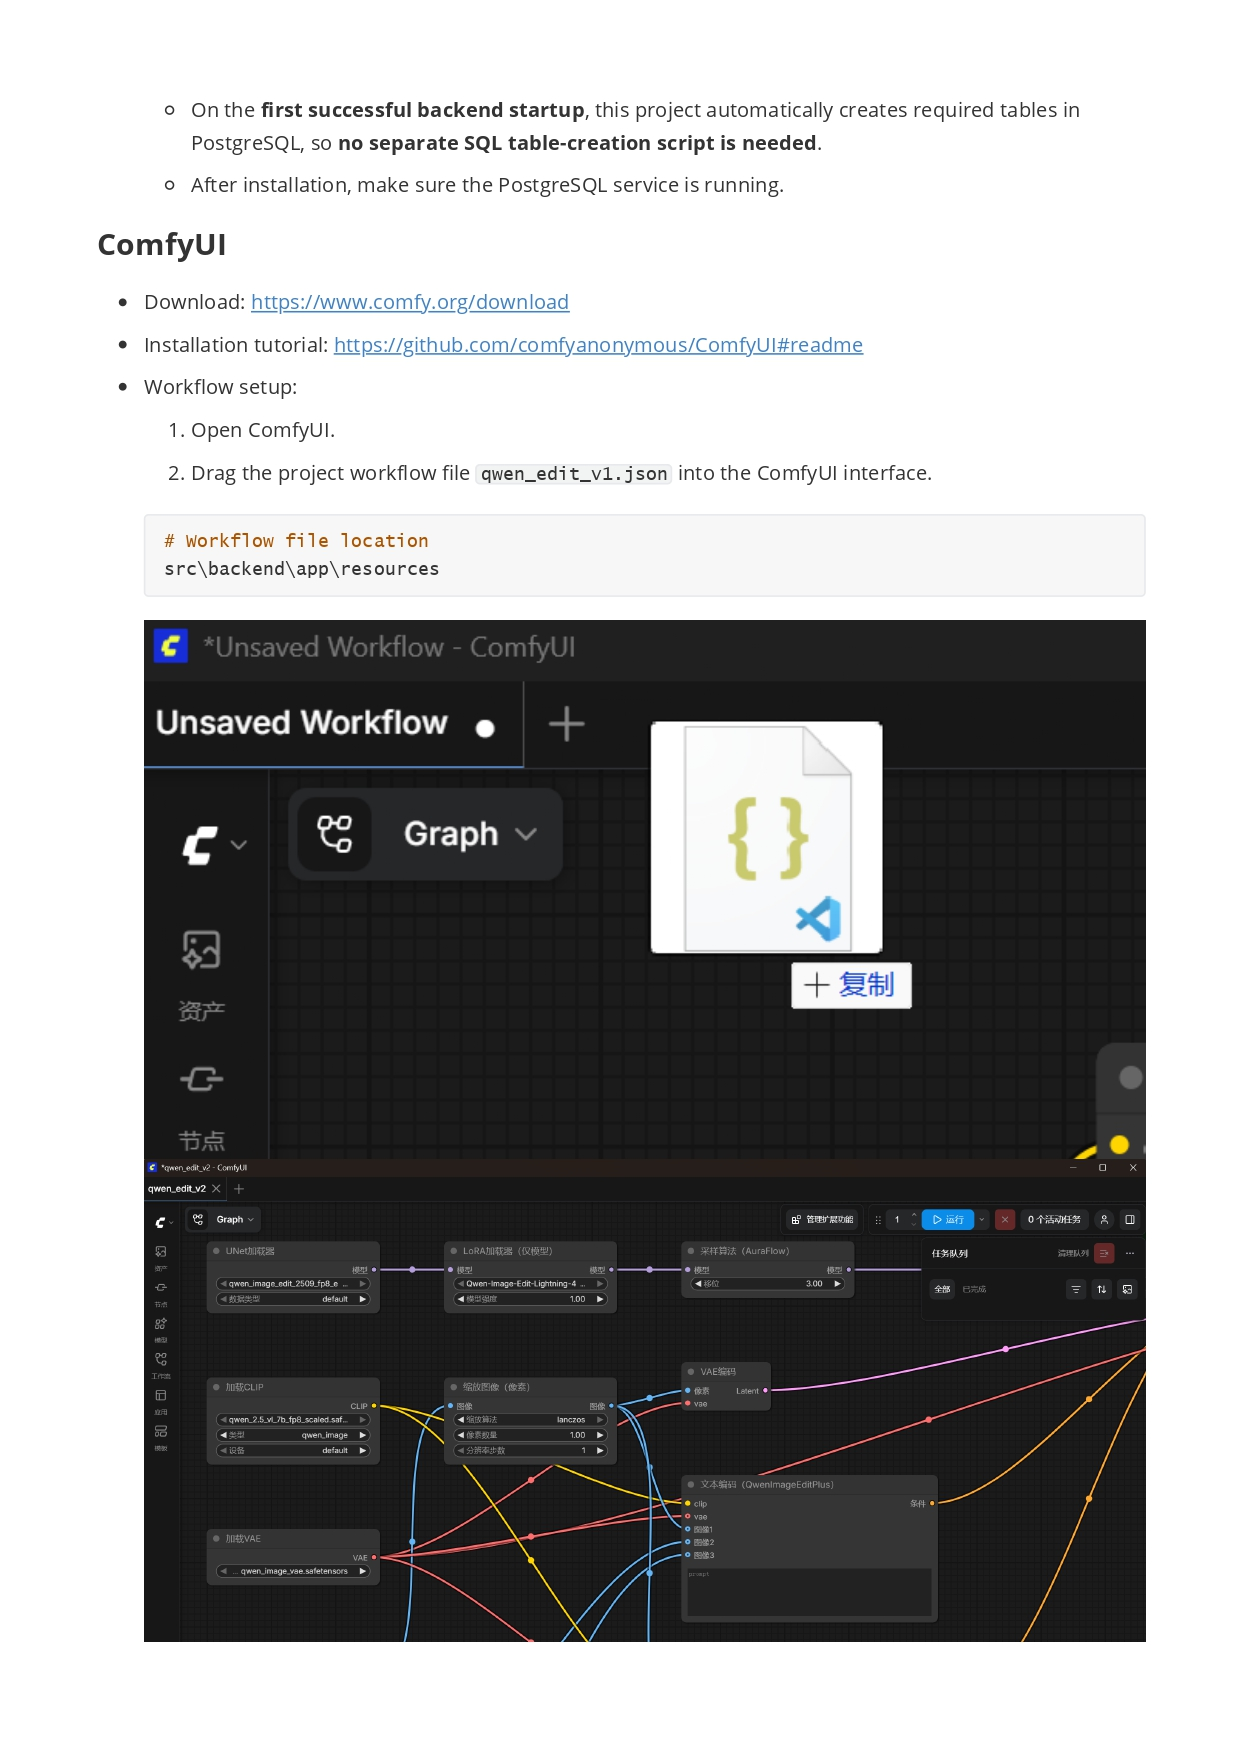
\includegraphics[width=0.95\textwidth]{images/appendix/install/installation_instruction_page-0002.jpg}
\end{figure}
\begin{figure}[H]
    \centering
    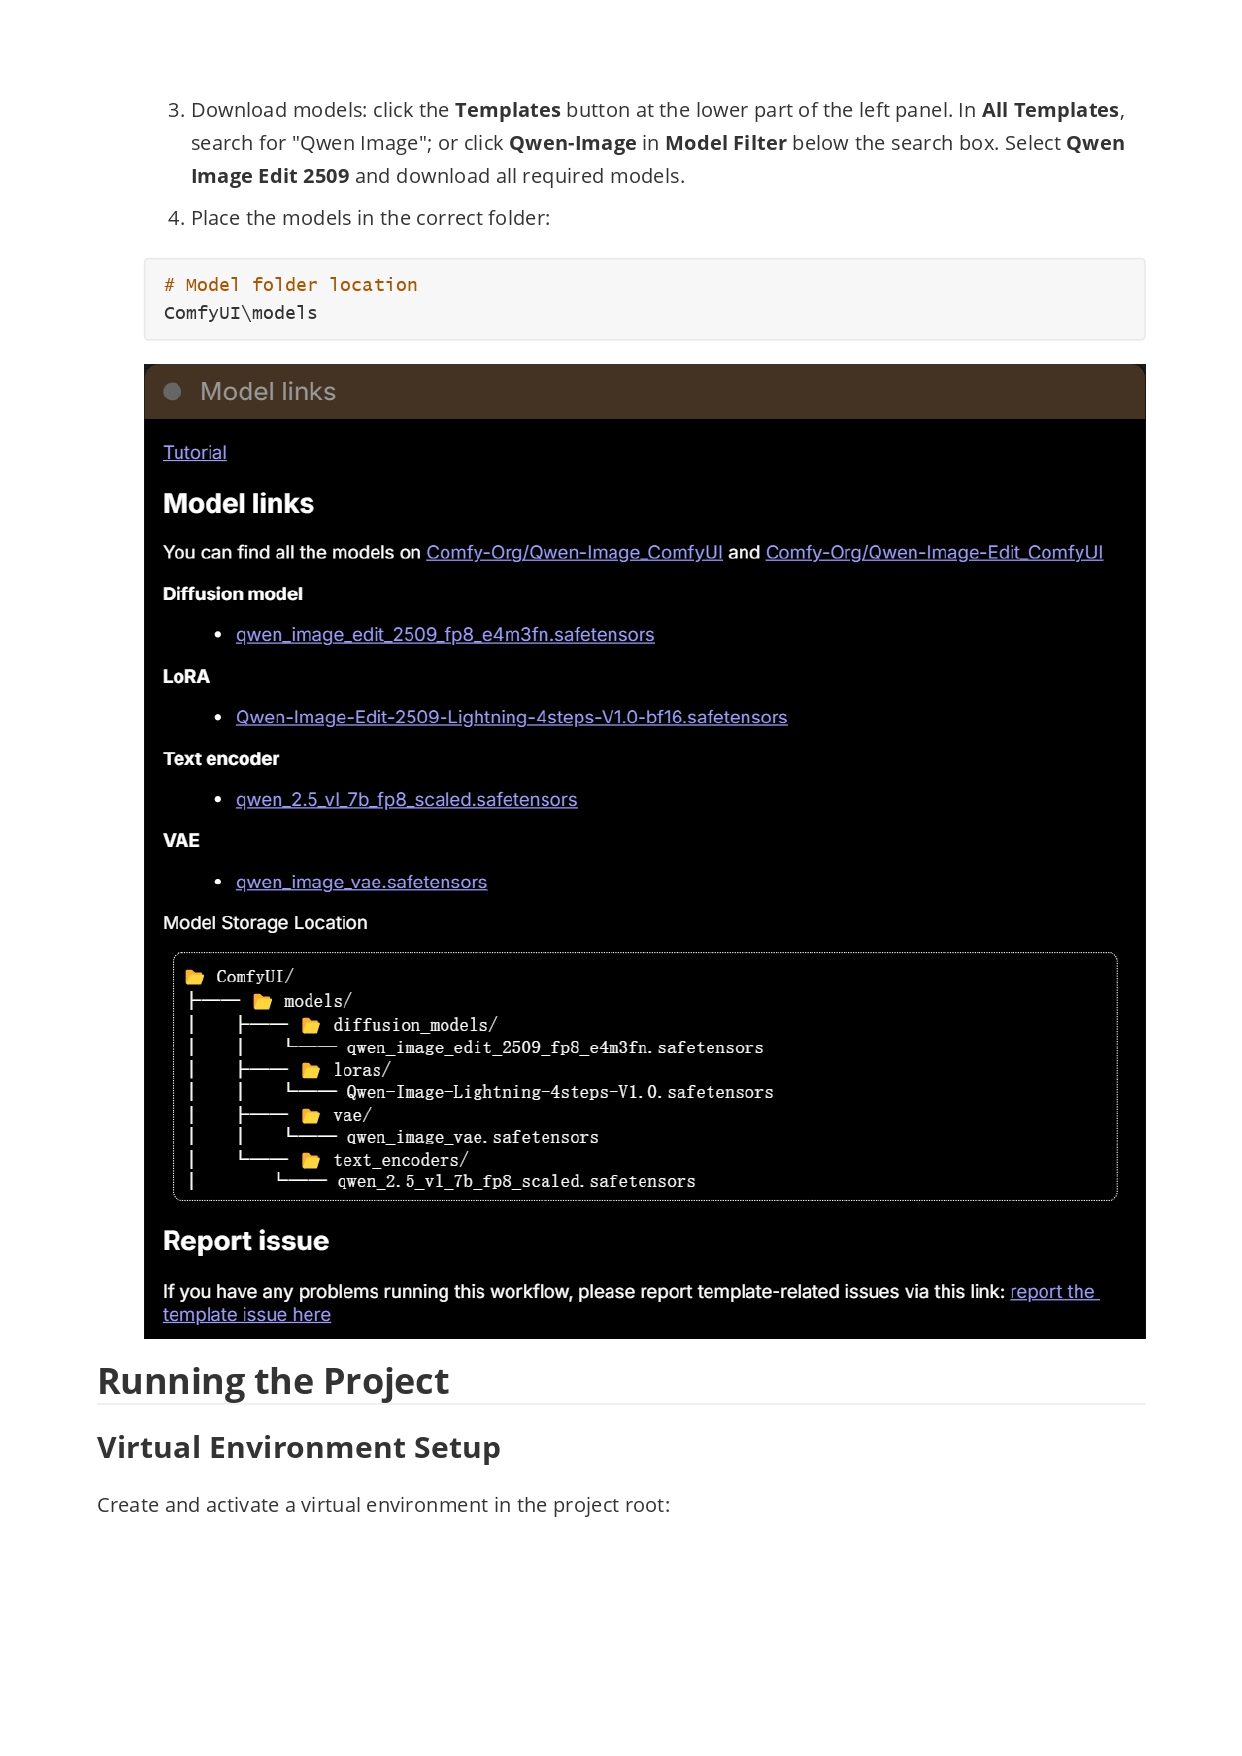
\includegraphics[width=1.0\textwidth]{images/appendix/install/installation_instruction_page-0003.jpg}
\end{figure}
\begin{figure}[H]
    \centering
    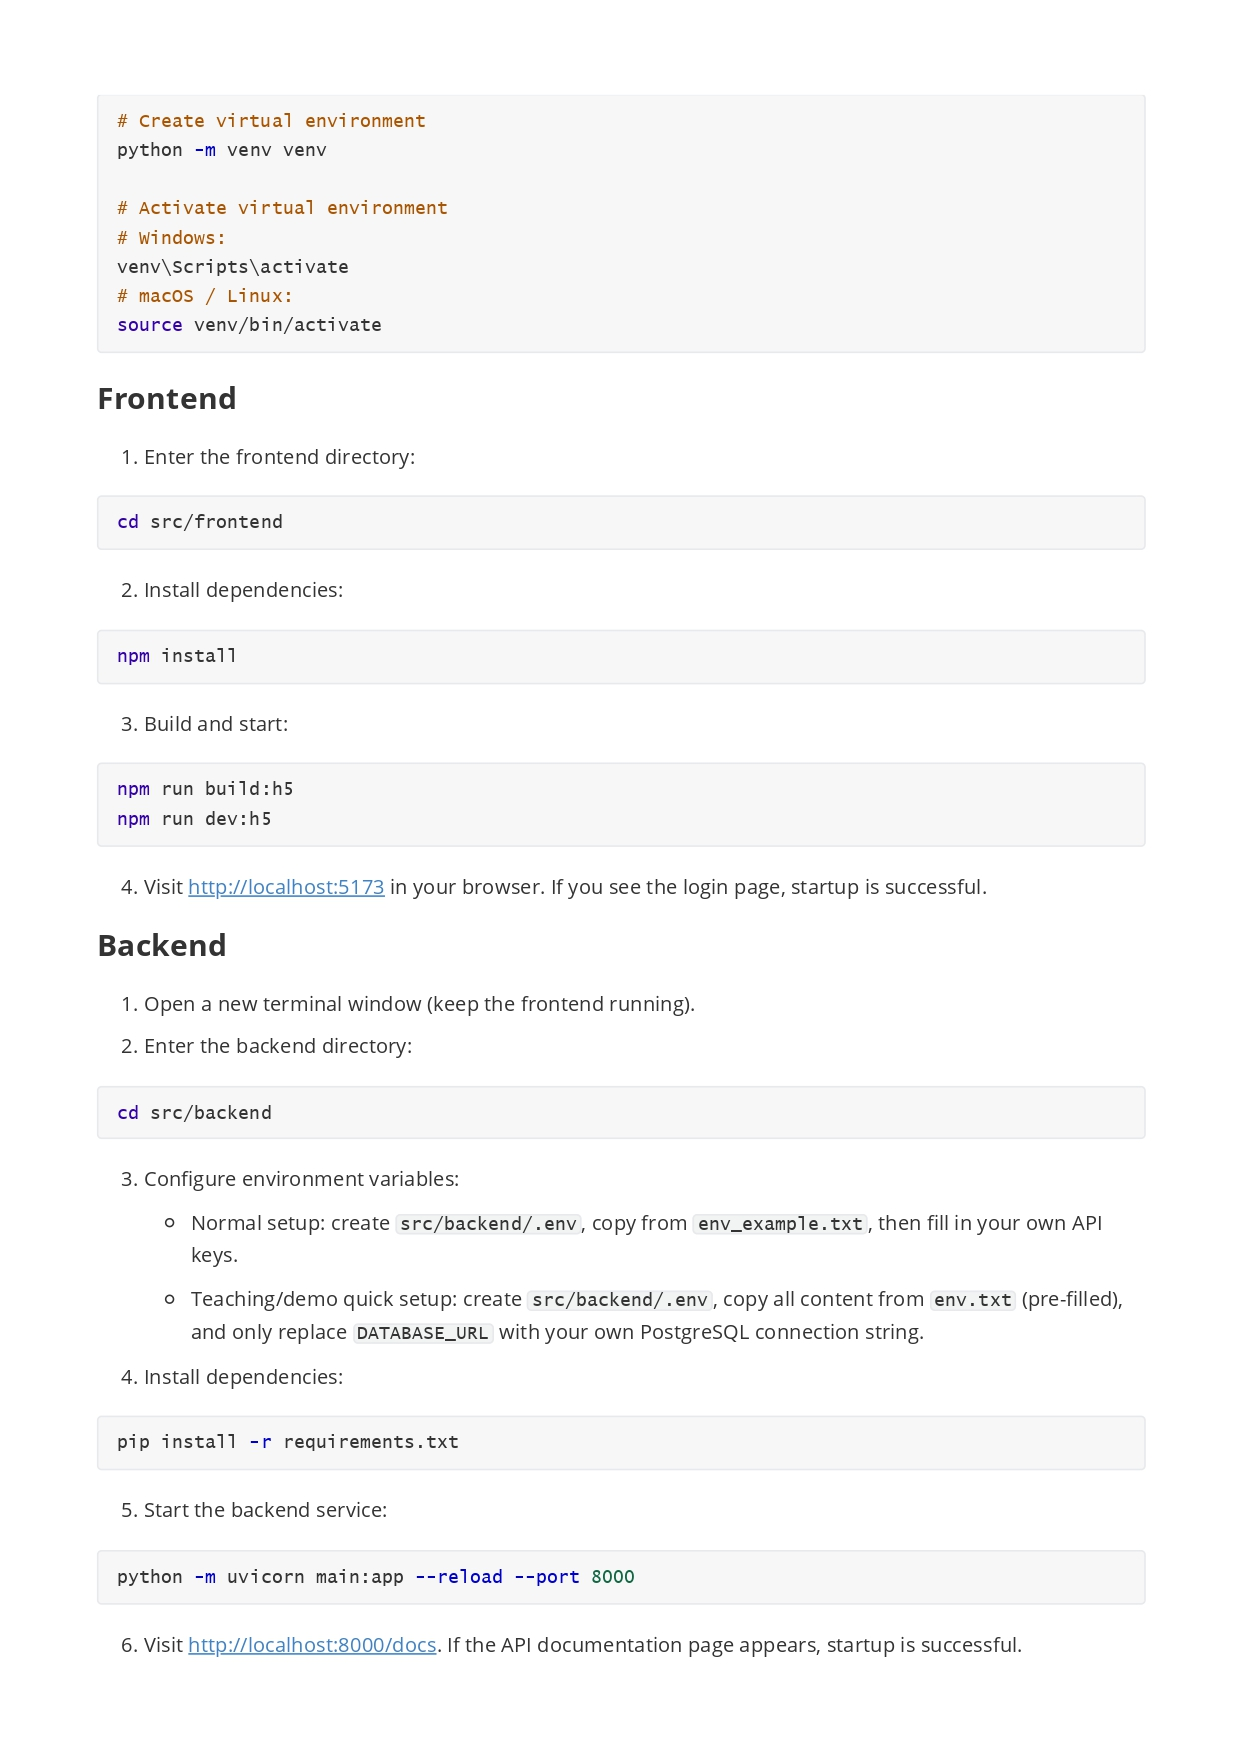
\includegraphics[width=1.0\textwidth]{images/appendix/install/installation_instruction_page-0004.jpg}
\end{figure}
\begin{figure}[H]
    \centering
    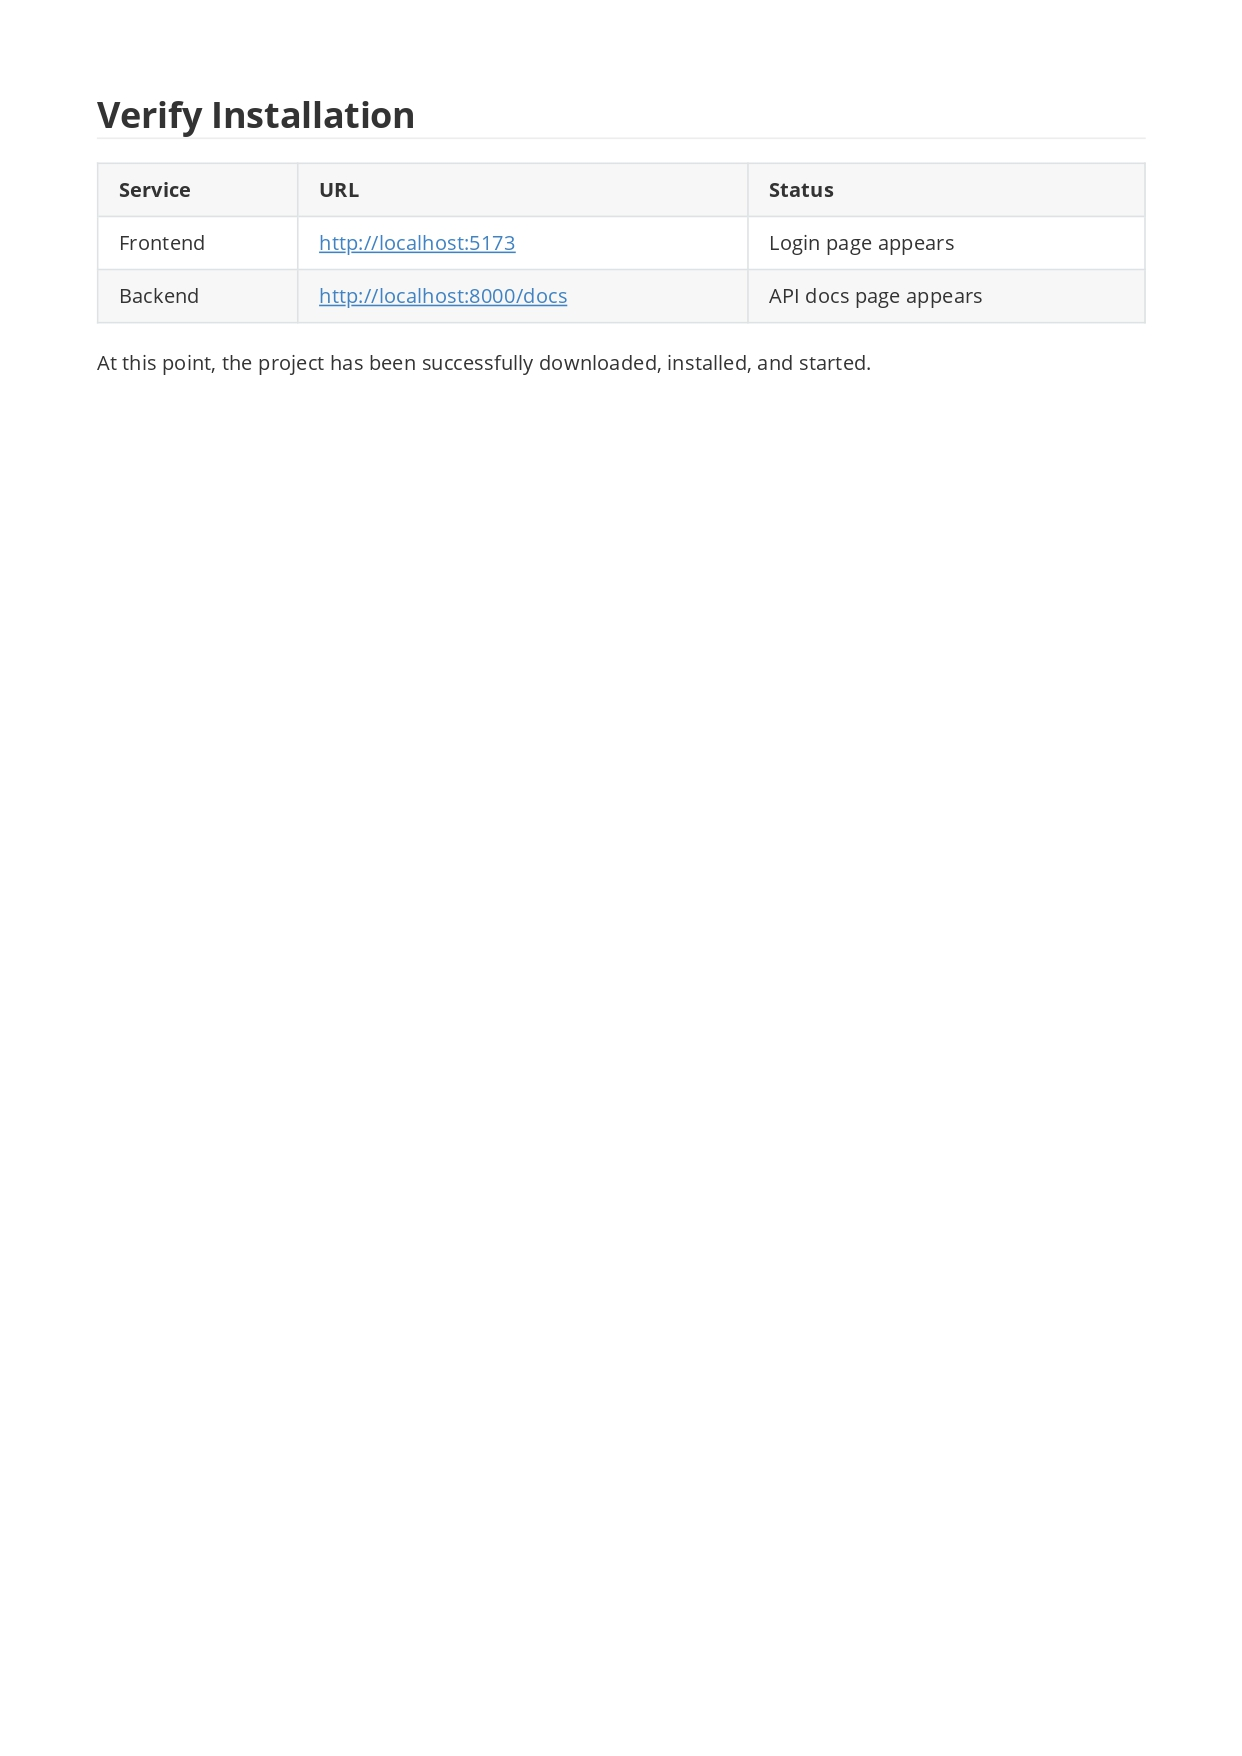
\includegraphics[width=1.0\textwidth]{images/appendix/install/installation_instruction_page-0005.jpg}
\end{figure}



\chapter{User Manual}
\label{appendix:user-manual}
\begin{figure}[H]
    \centering
    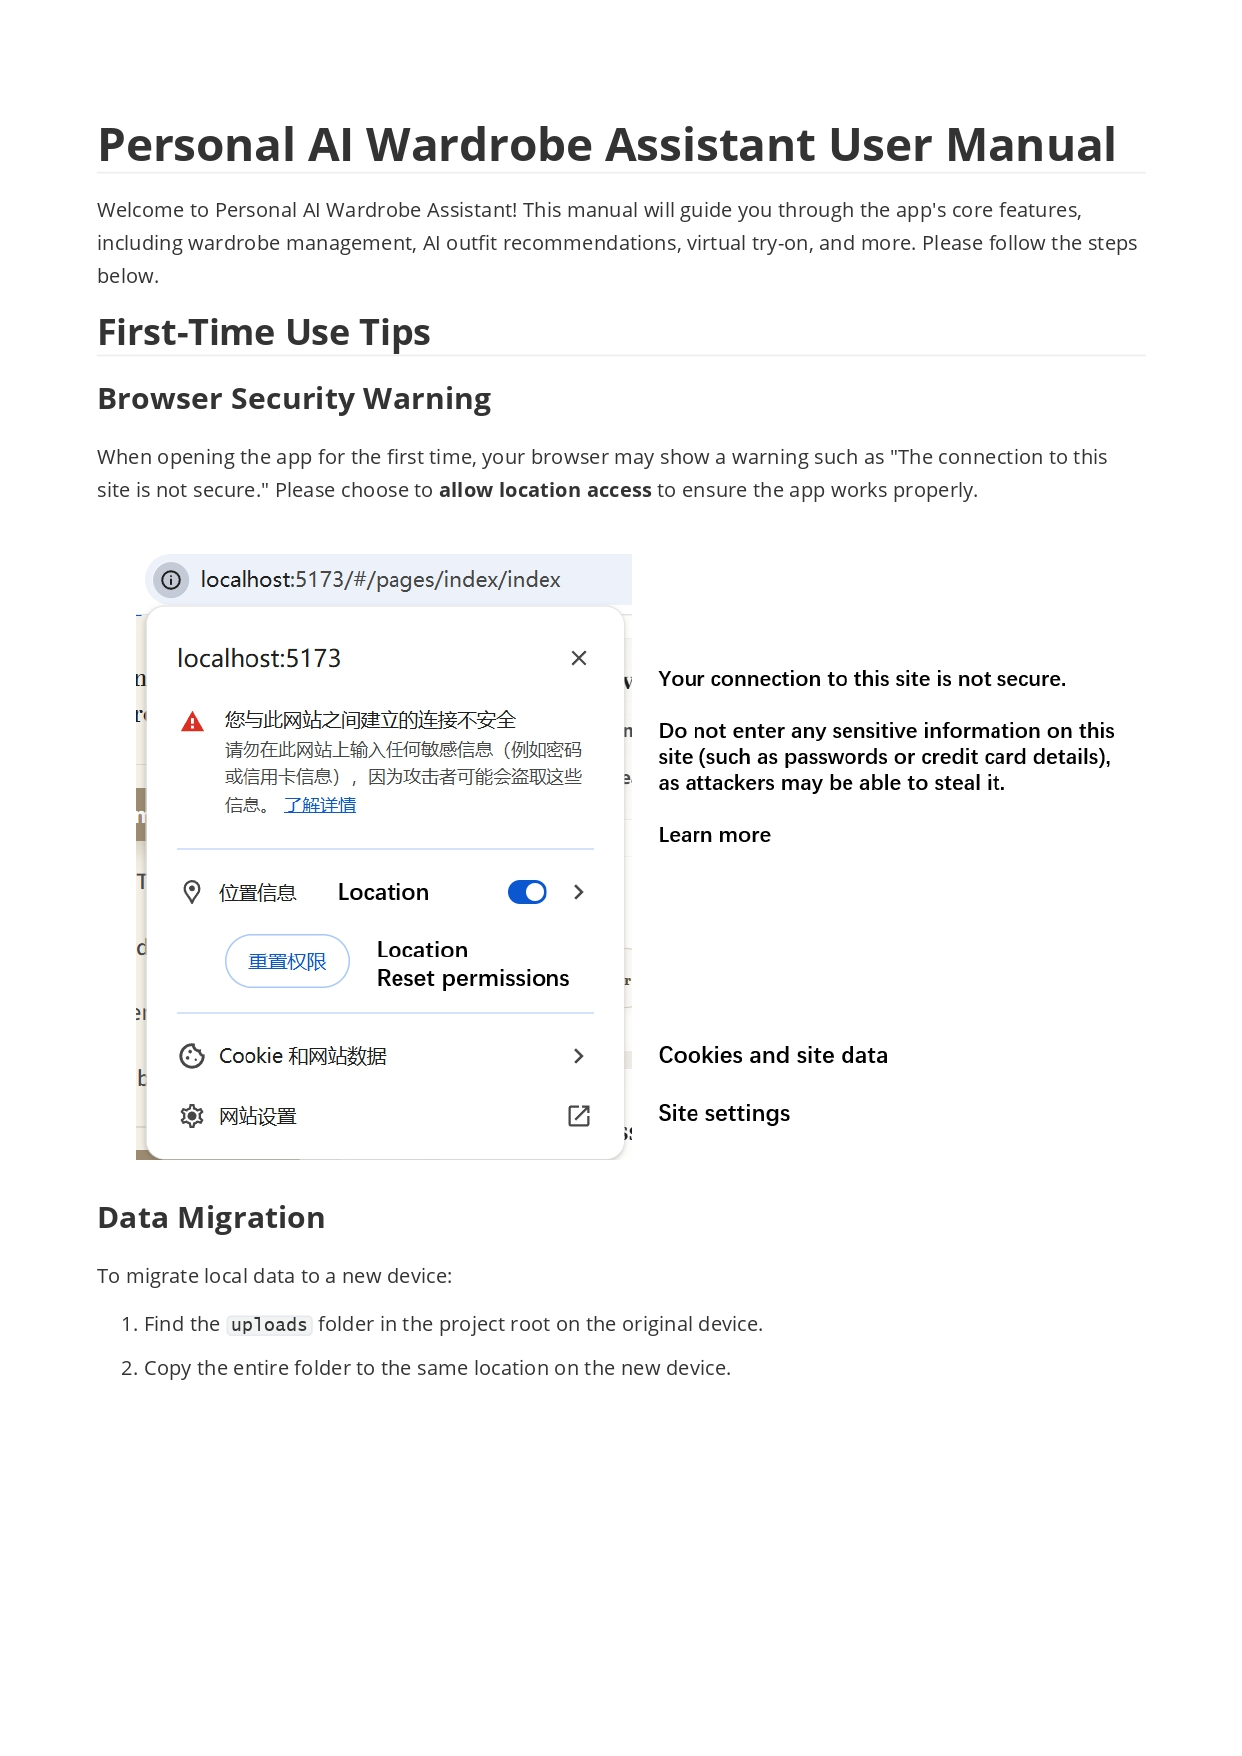
\includegraphics[width=1.0\textwidth]{images/appendix/user-manual/user_manual_page-0001.jpg}
\end{figure}
\begin{figure}[H]
    \centering
    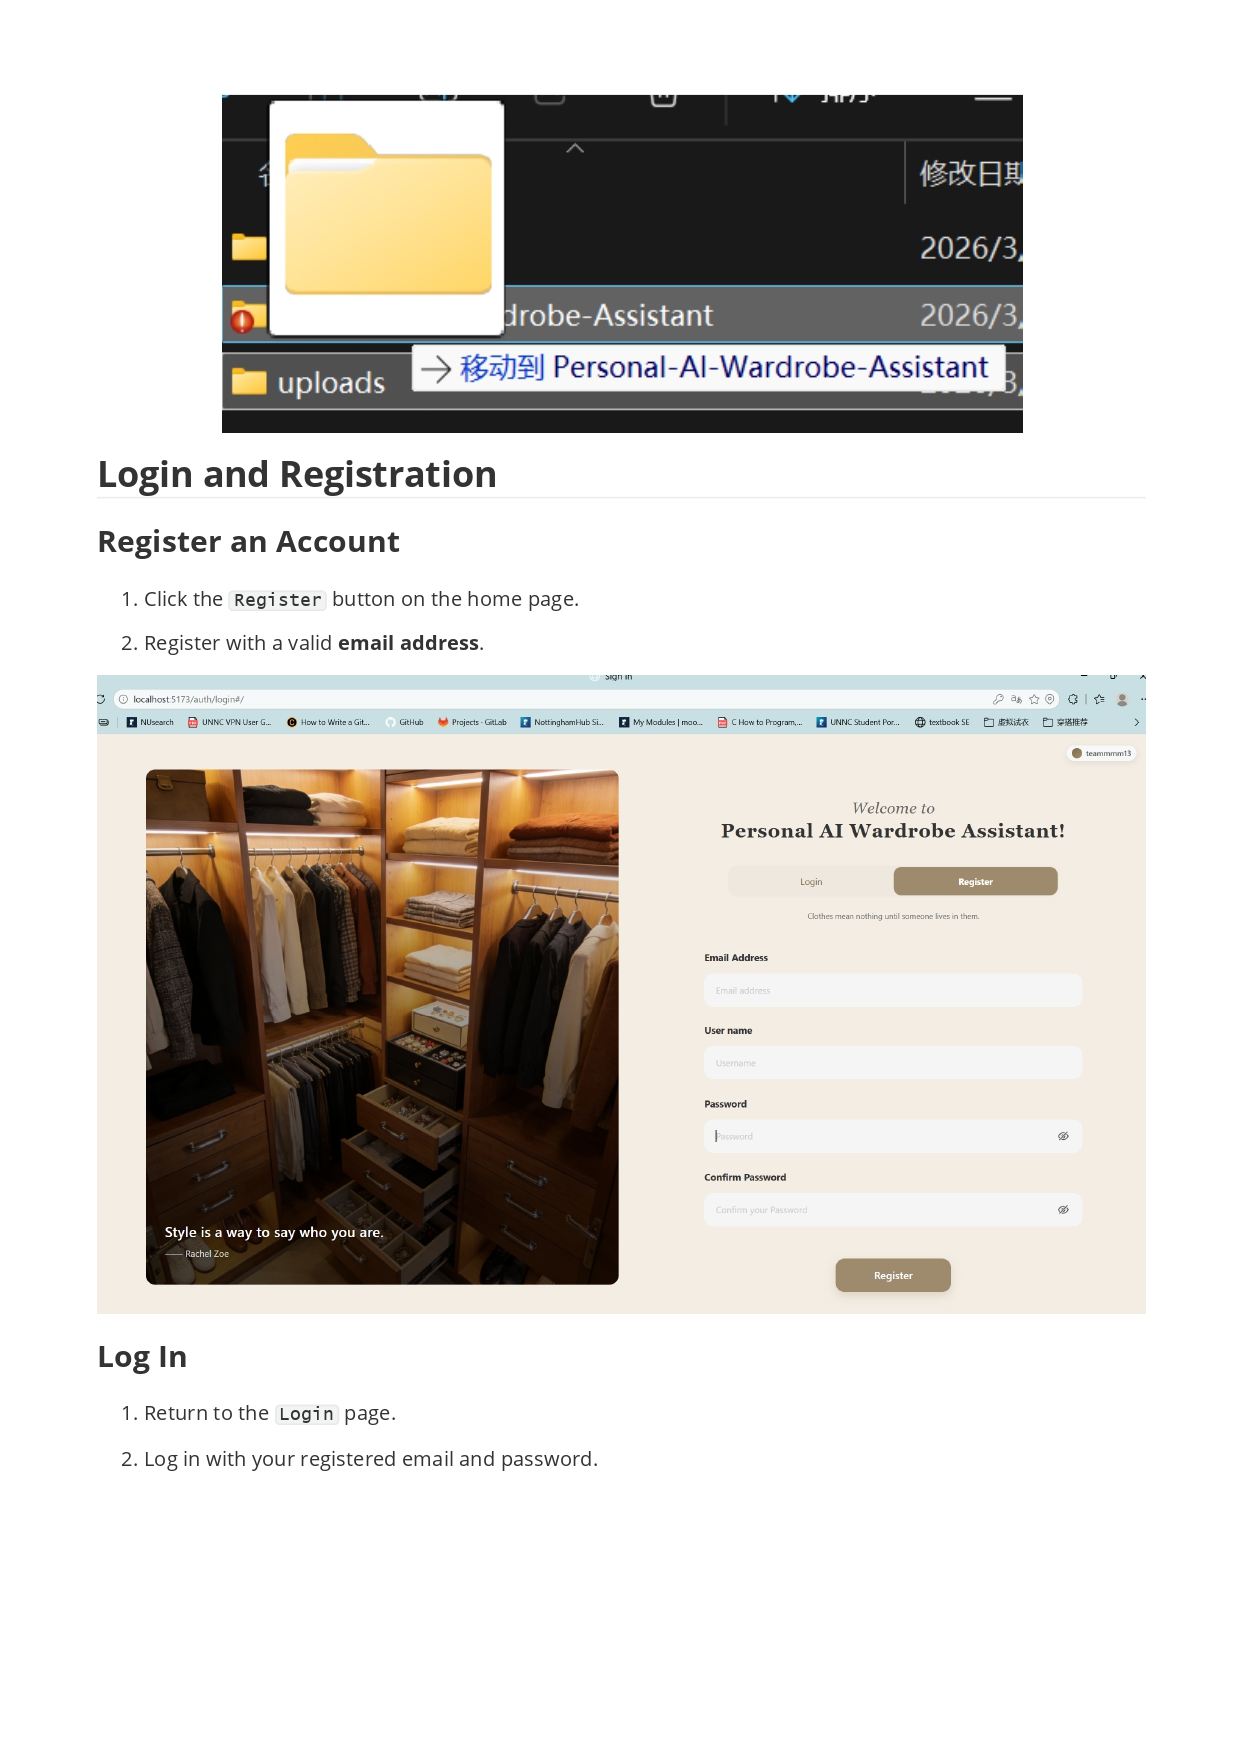
\includegraphics[width=1.0\textwidth]{images/appendix/user-manual/user_manual_page-0002.jpg}
\end{figure}
\begin{figure}[H]
    \centering
    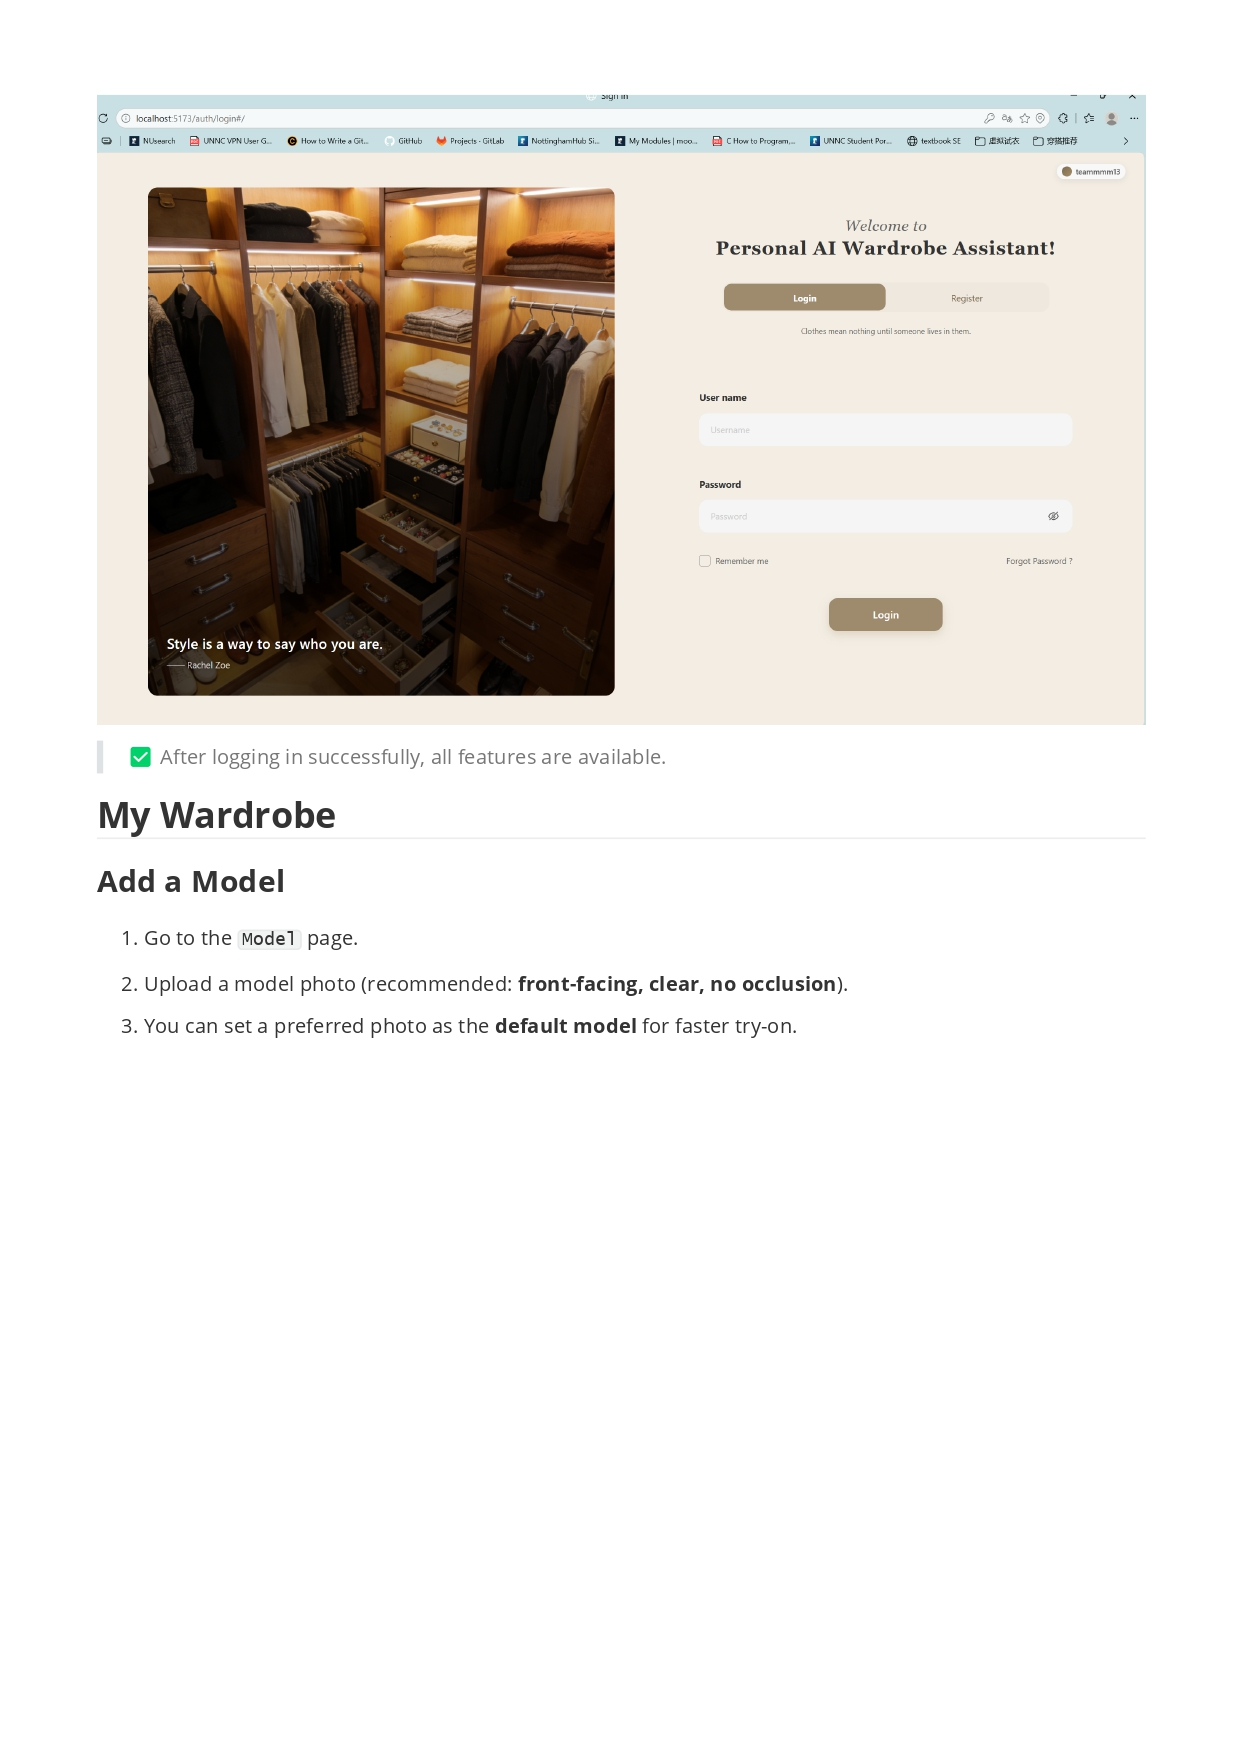
\includegraphics[width=1.0\textwidth]{images/appendix/user-manual/user_manual_page-0003.jpg}
\end{figure}
\begin{figure}[H]
    \centering
    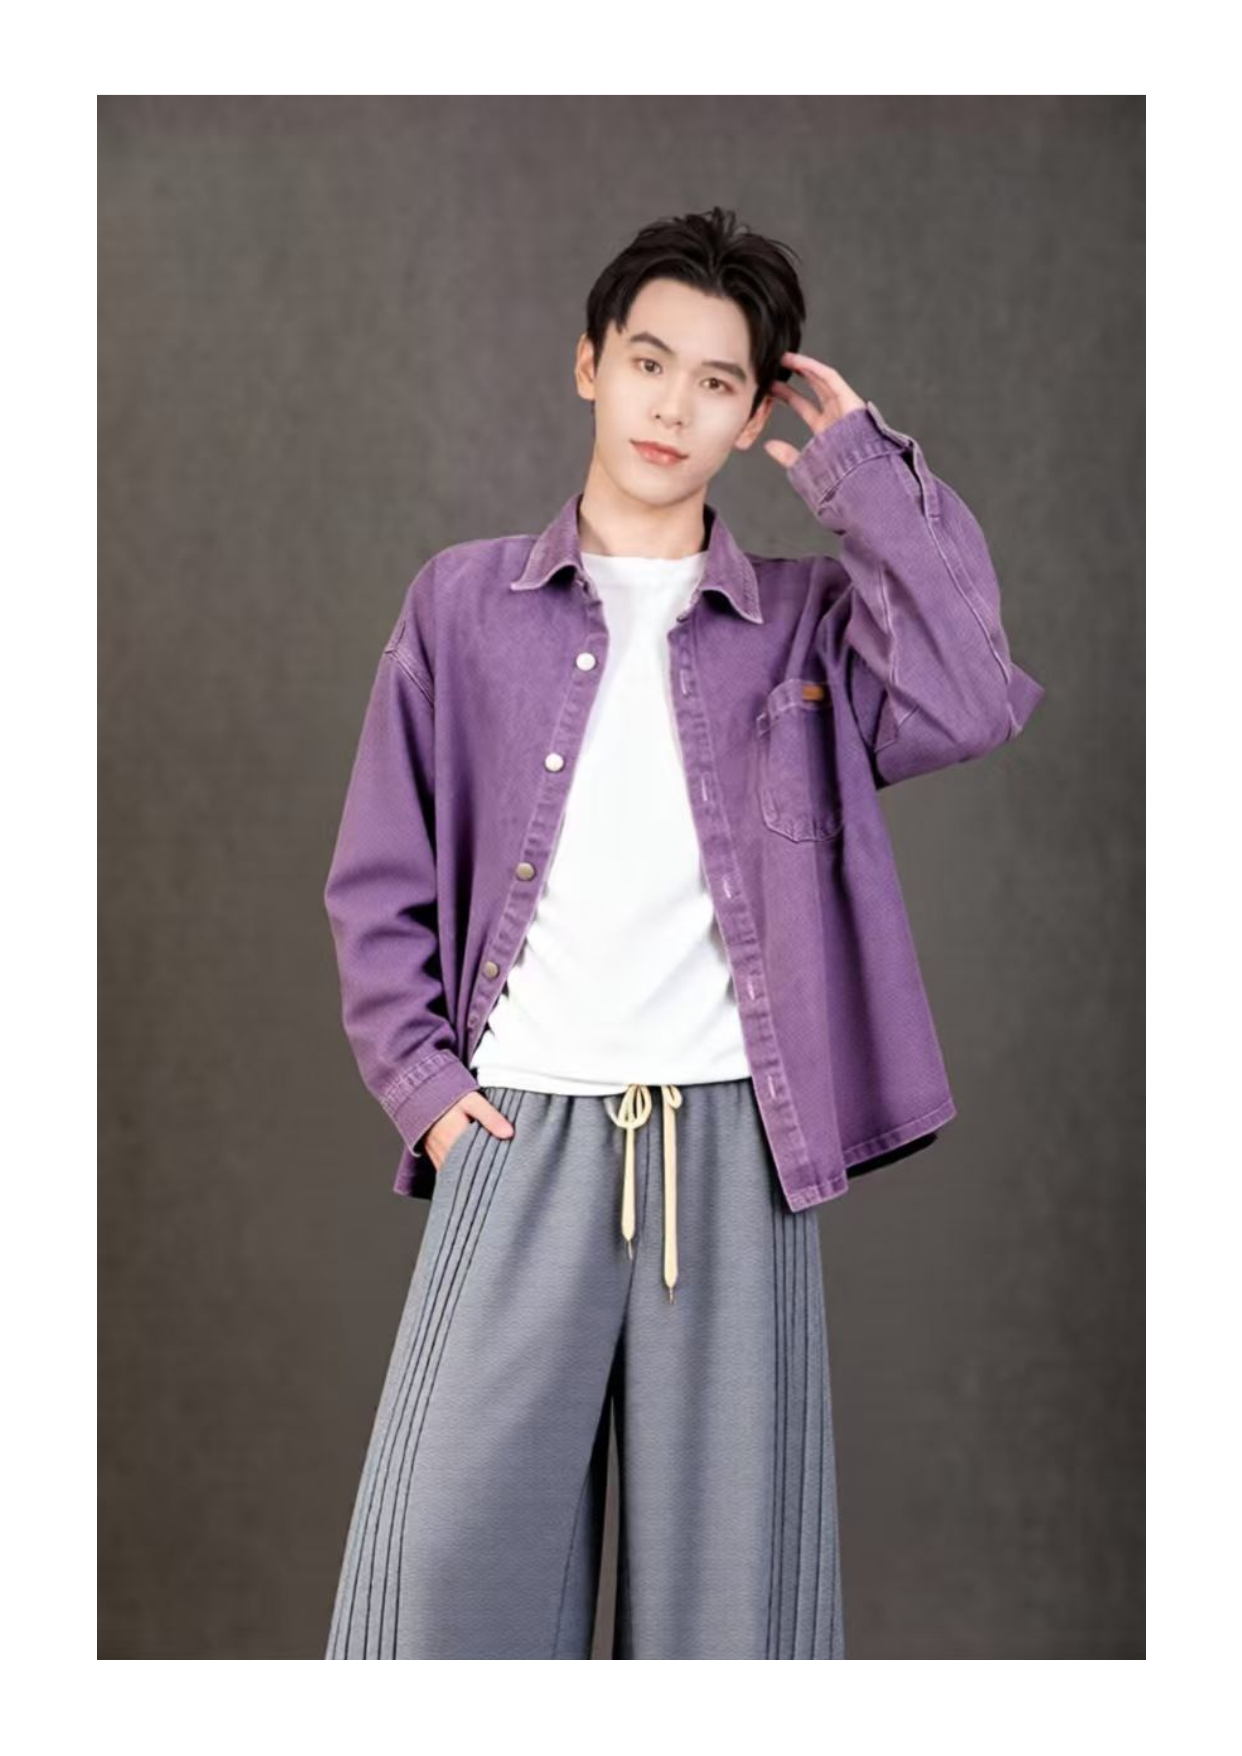
\includegraphics[width=1.0\textwidth]{images/appendix/user-manual/user_manual_page-0004.jpg}
\end{figure}
\begin{figure}[H]
    \centering
    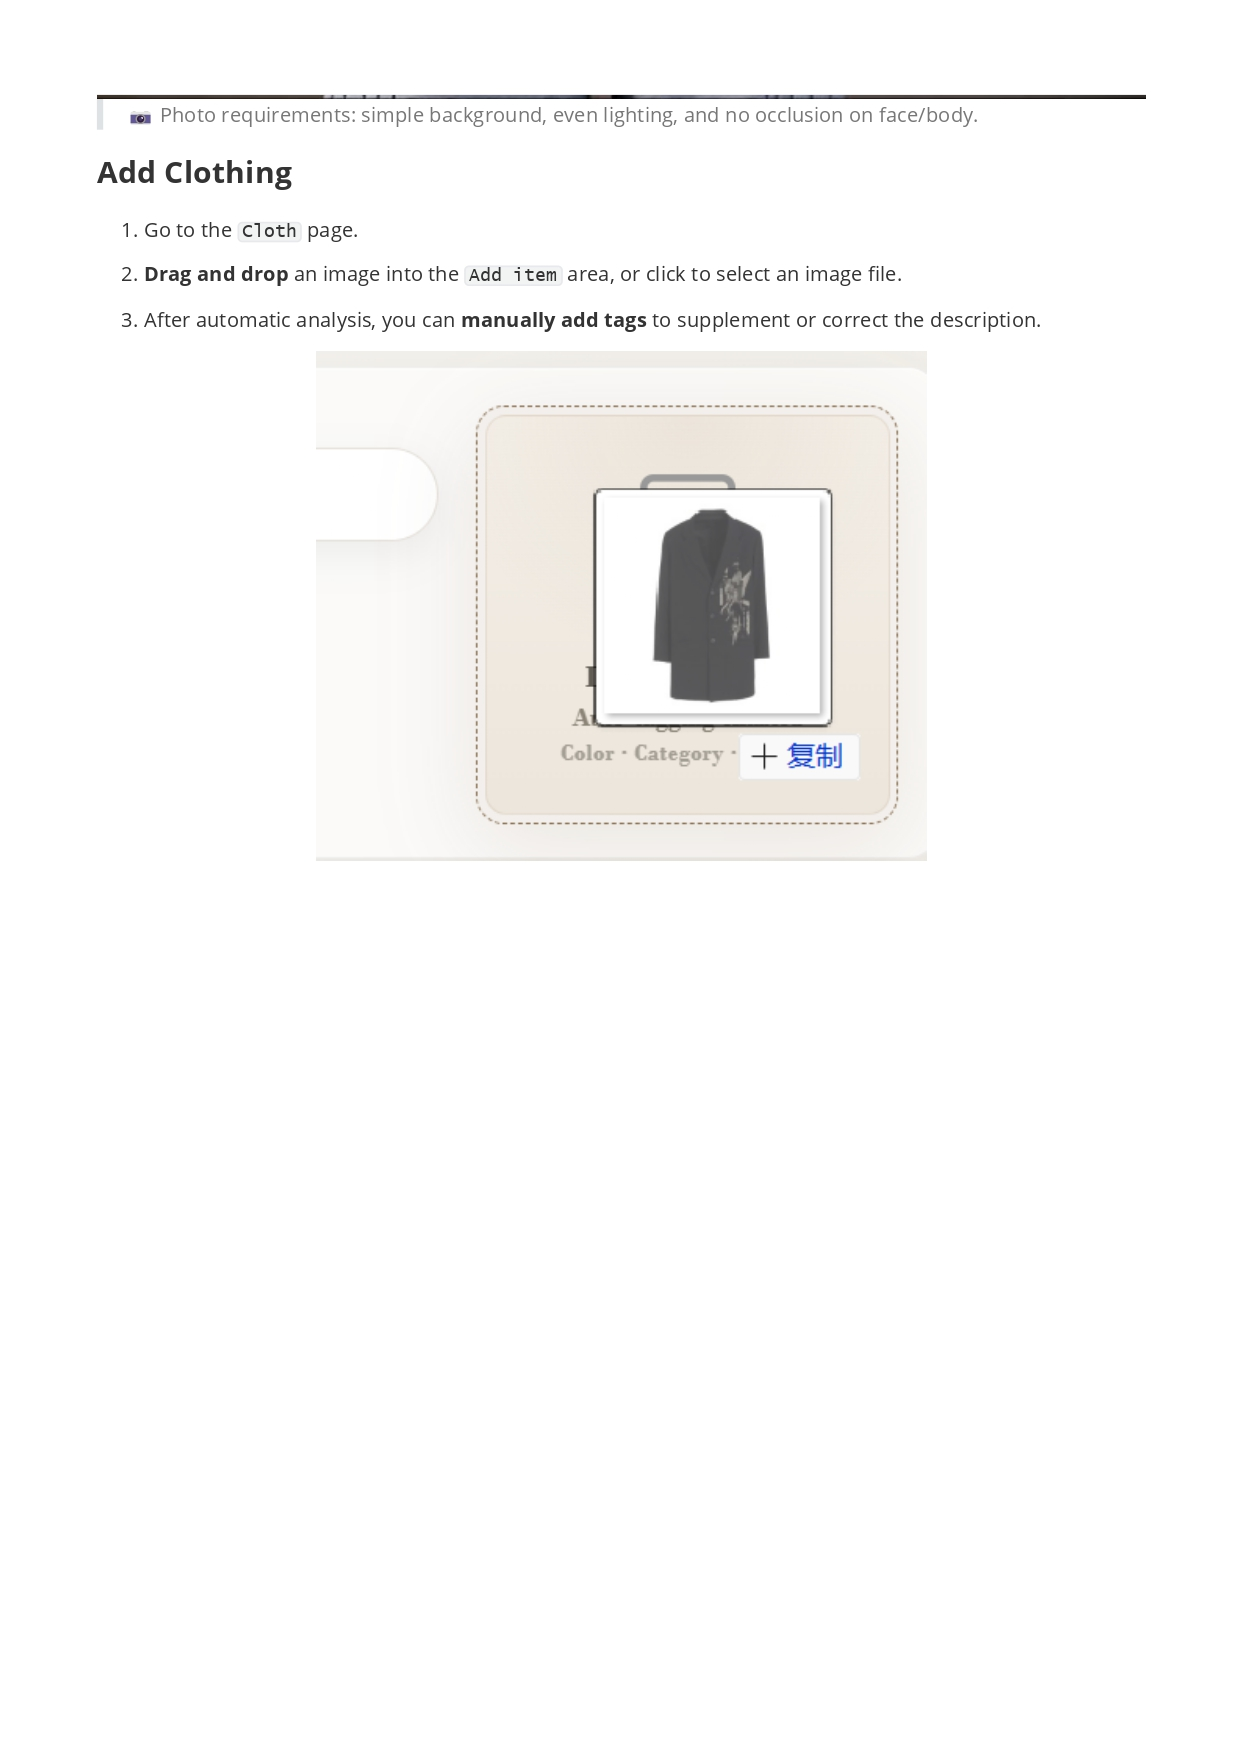
\includegraphics[width=1.0\textwidth]{images/appendix/user-manual/user_manual_page-0005.jpg}
\end{figure}
\begin{figure}[H]
    \centering
    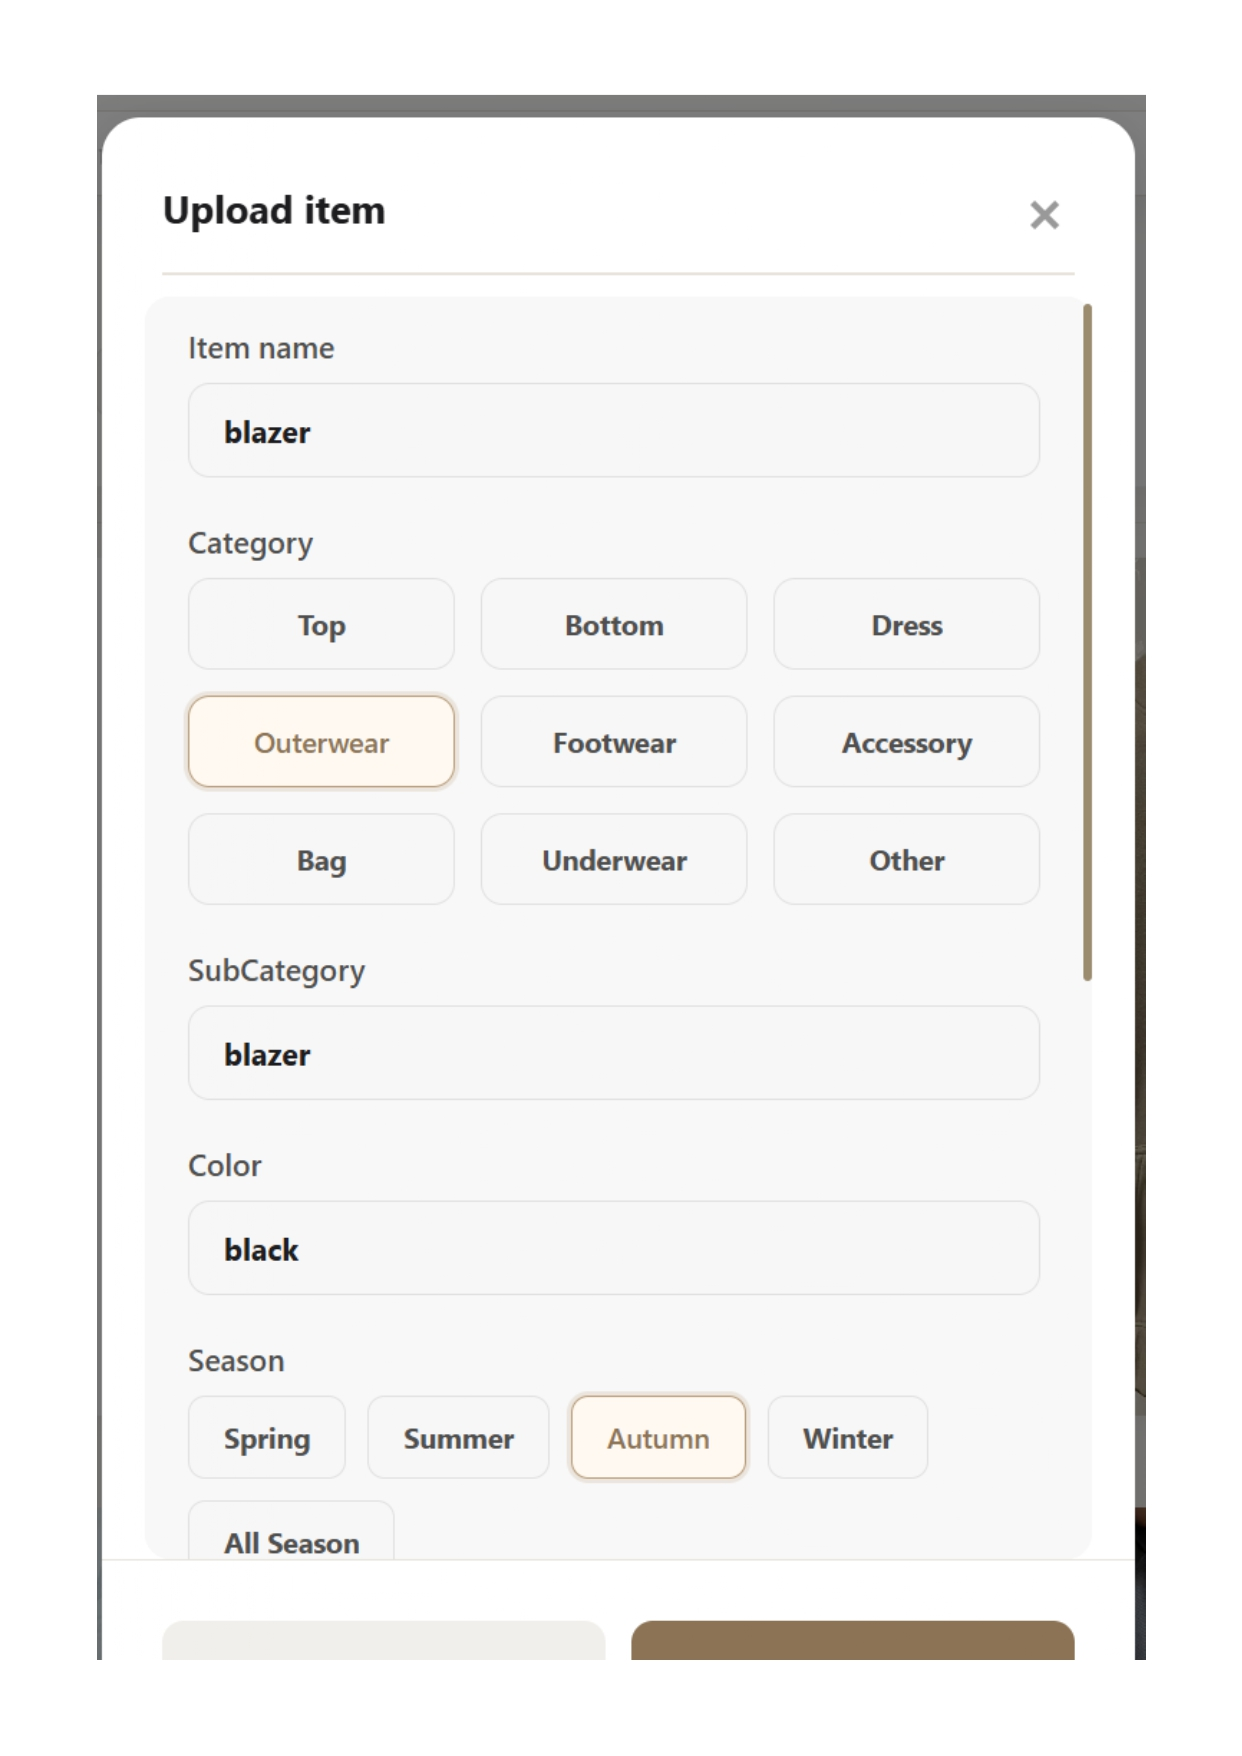
\includegraphics[width=1.0\textwidth]{images/appendix/user-manual/user_manual_page-0006.jpg}
\end{figure}
\begin{figure}[H]
    \centering
    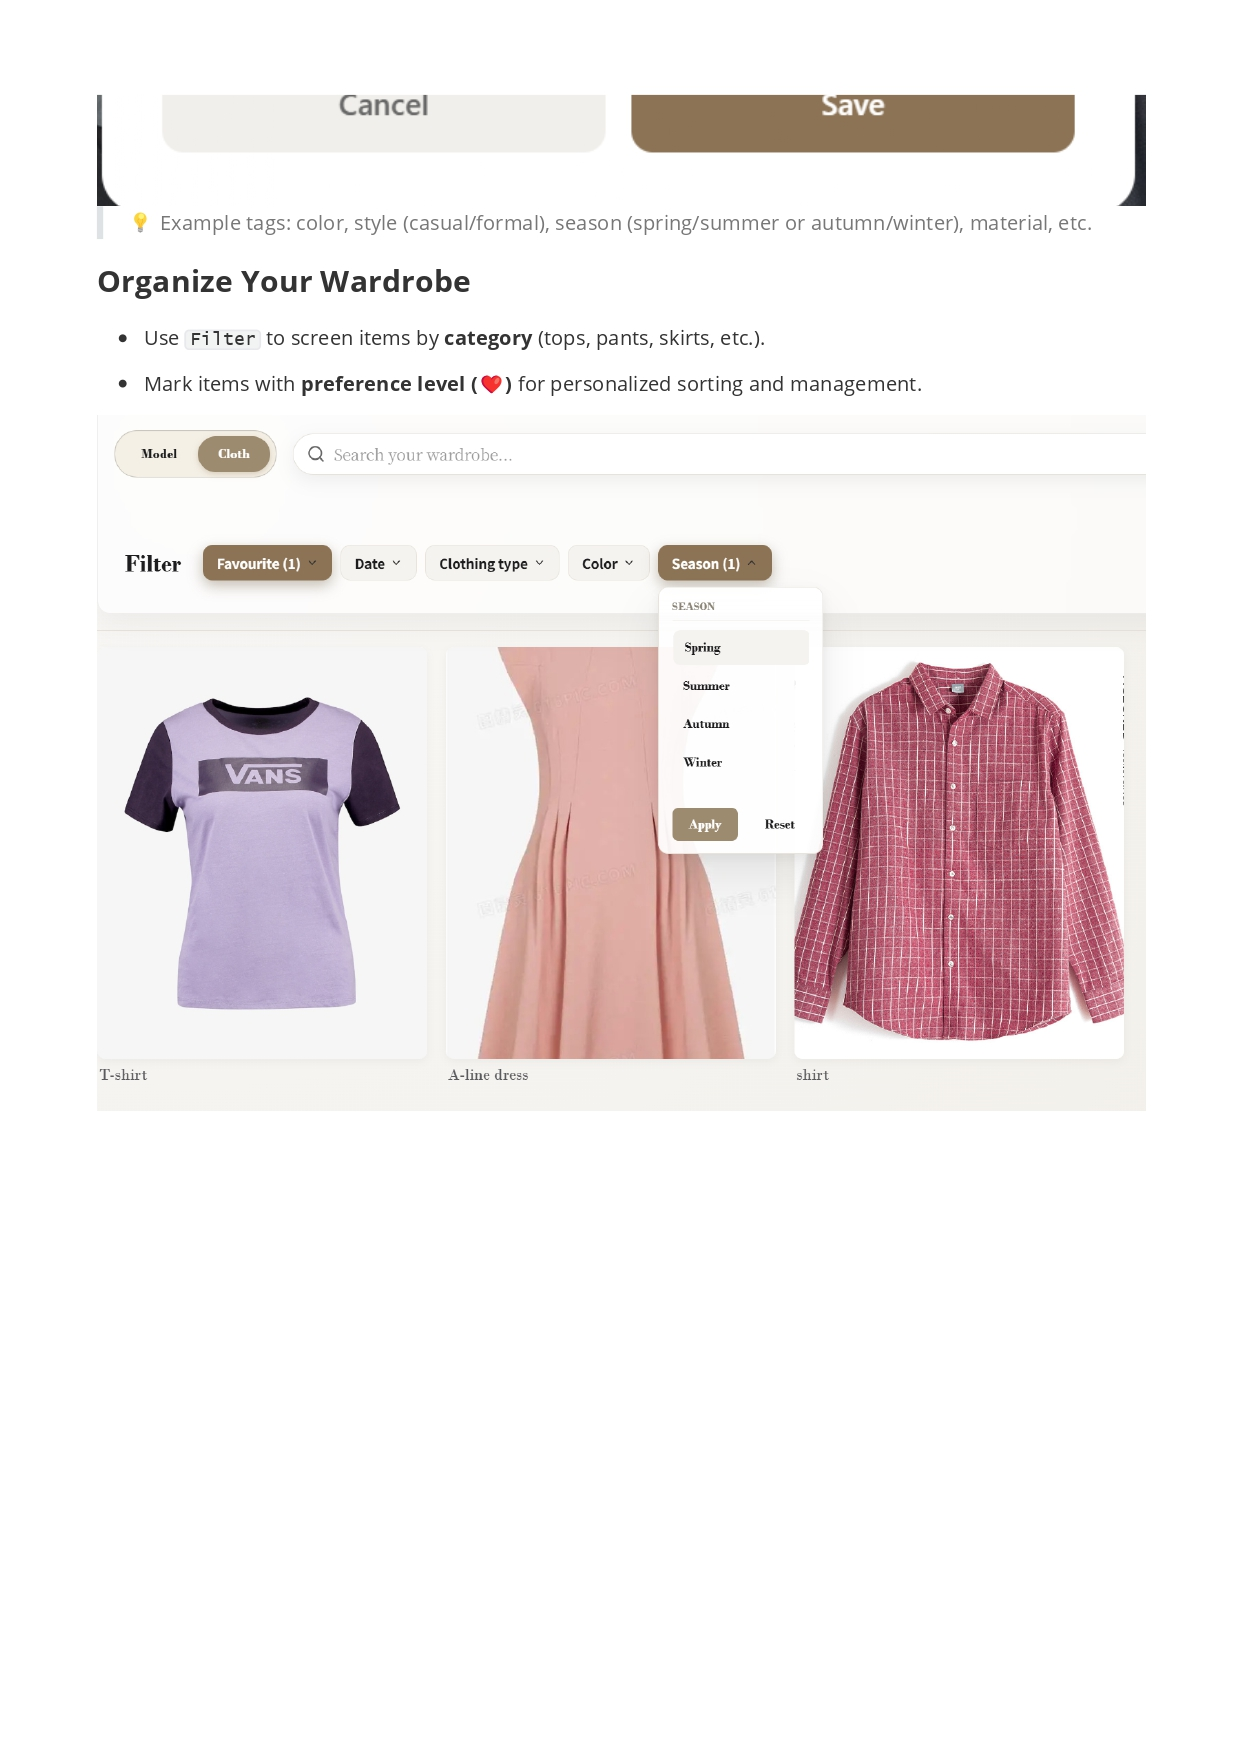
\includegraphics[width=1.0\textwidth]{images/appendix/user-manual/user_manual_page-0007.jpg}
\end{figure}
\begin{figure}[H]
    \centering
    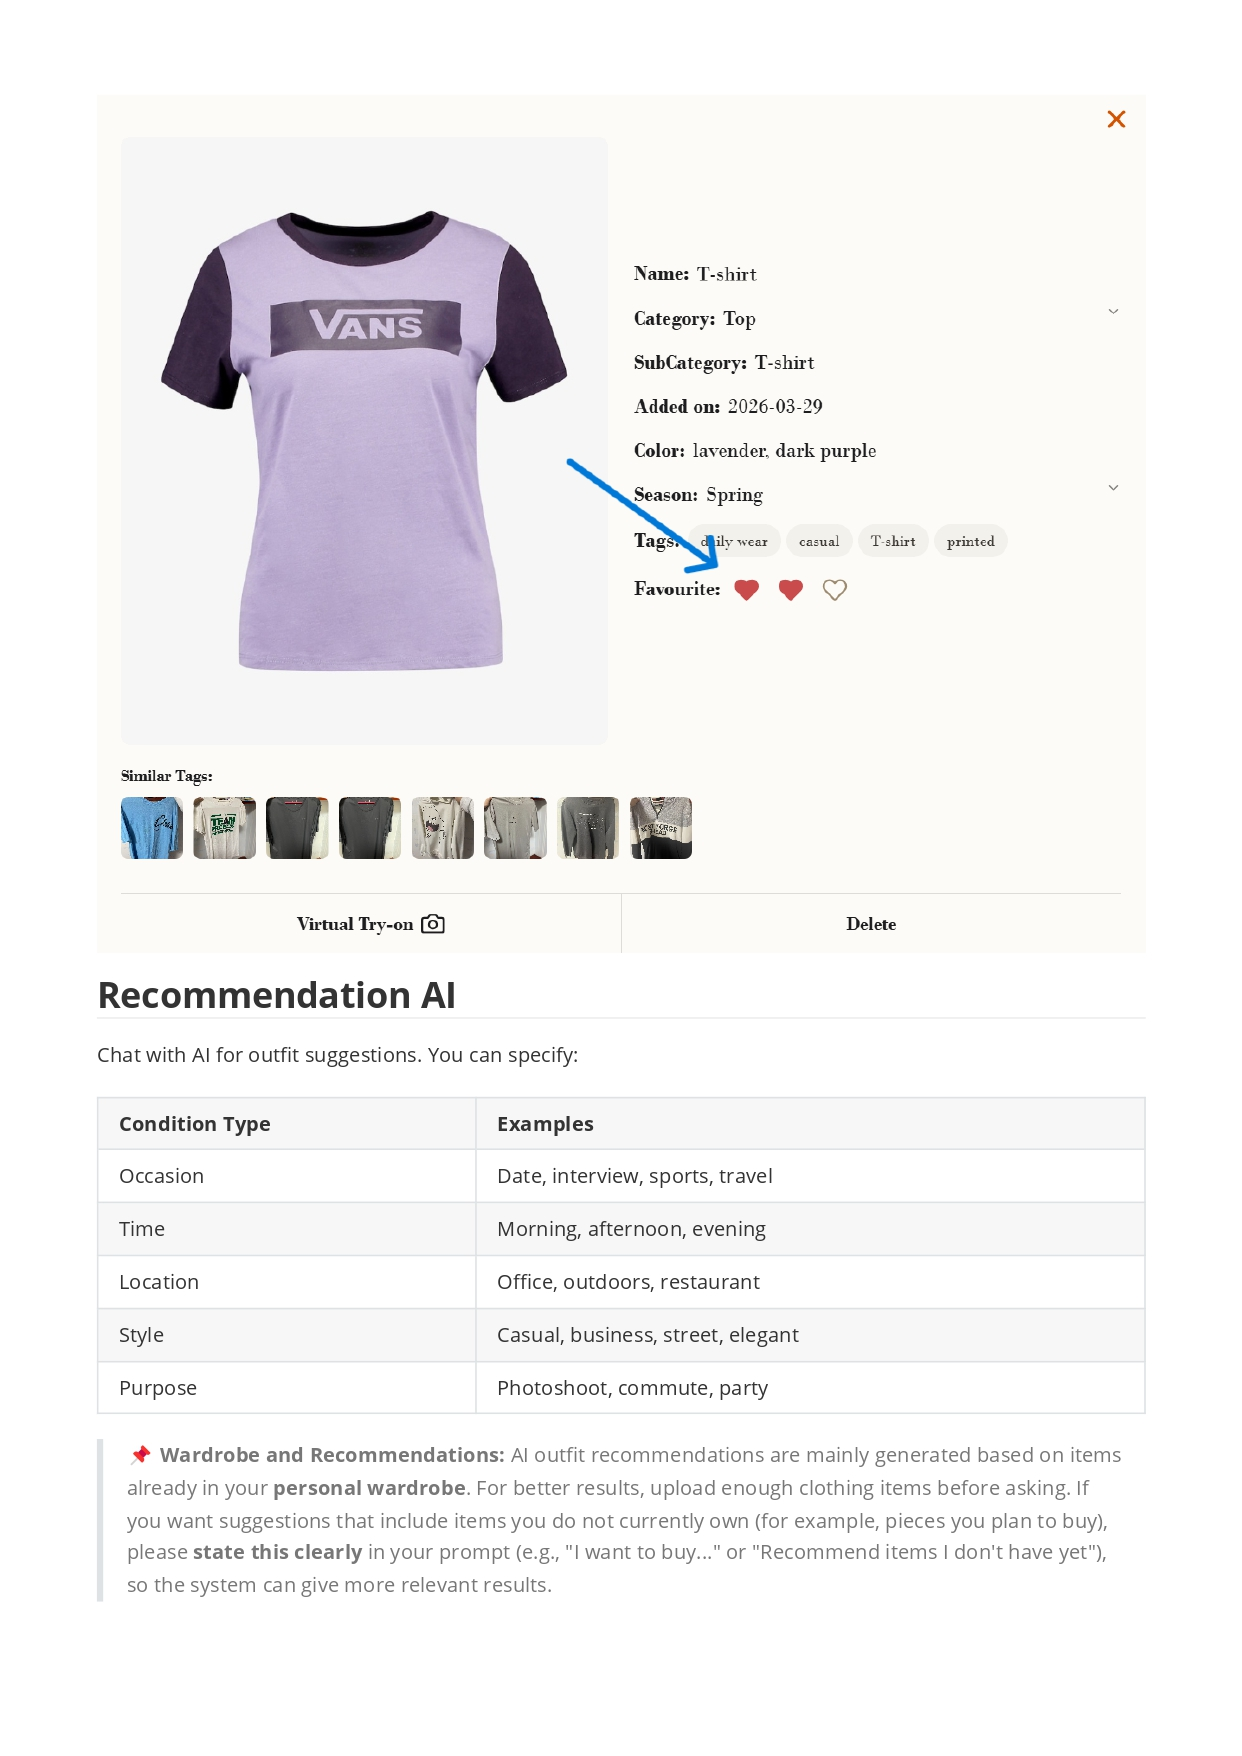
\includegraphics[width=1.0\textwidth]{images/appendix/user-manual/user_manual_page-0008.jpg}
\end{figure}
\begin{figure}[H]
    \centering
    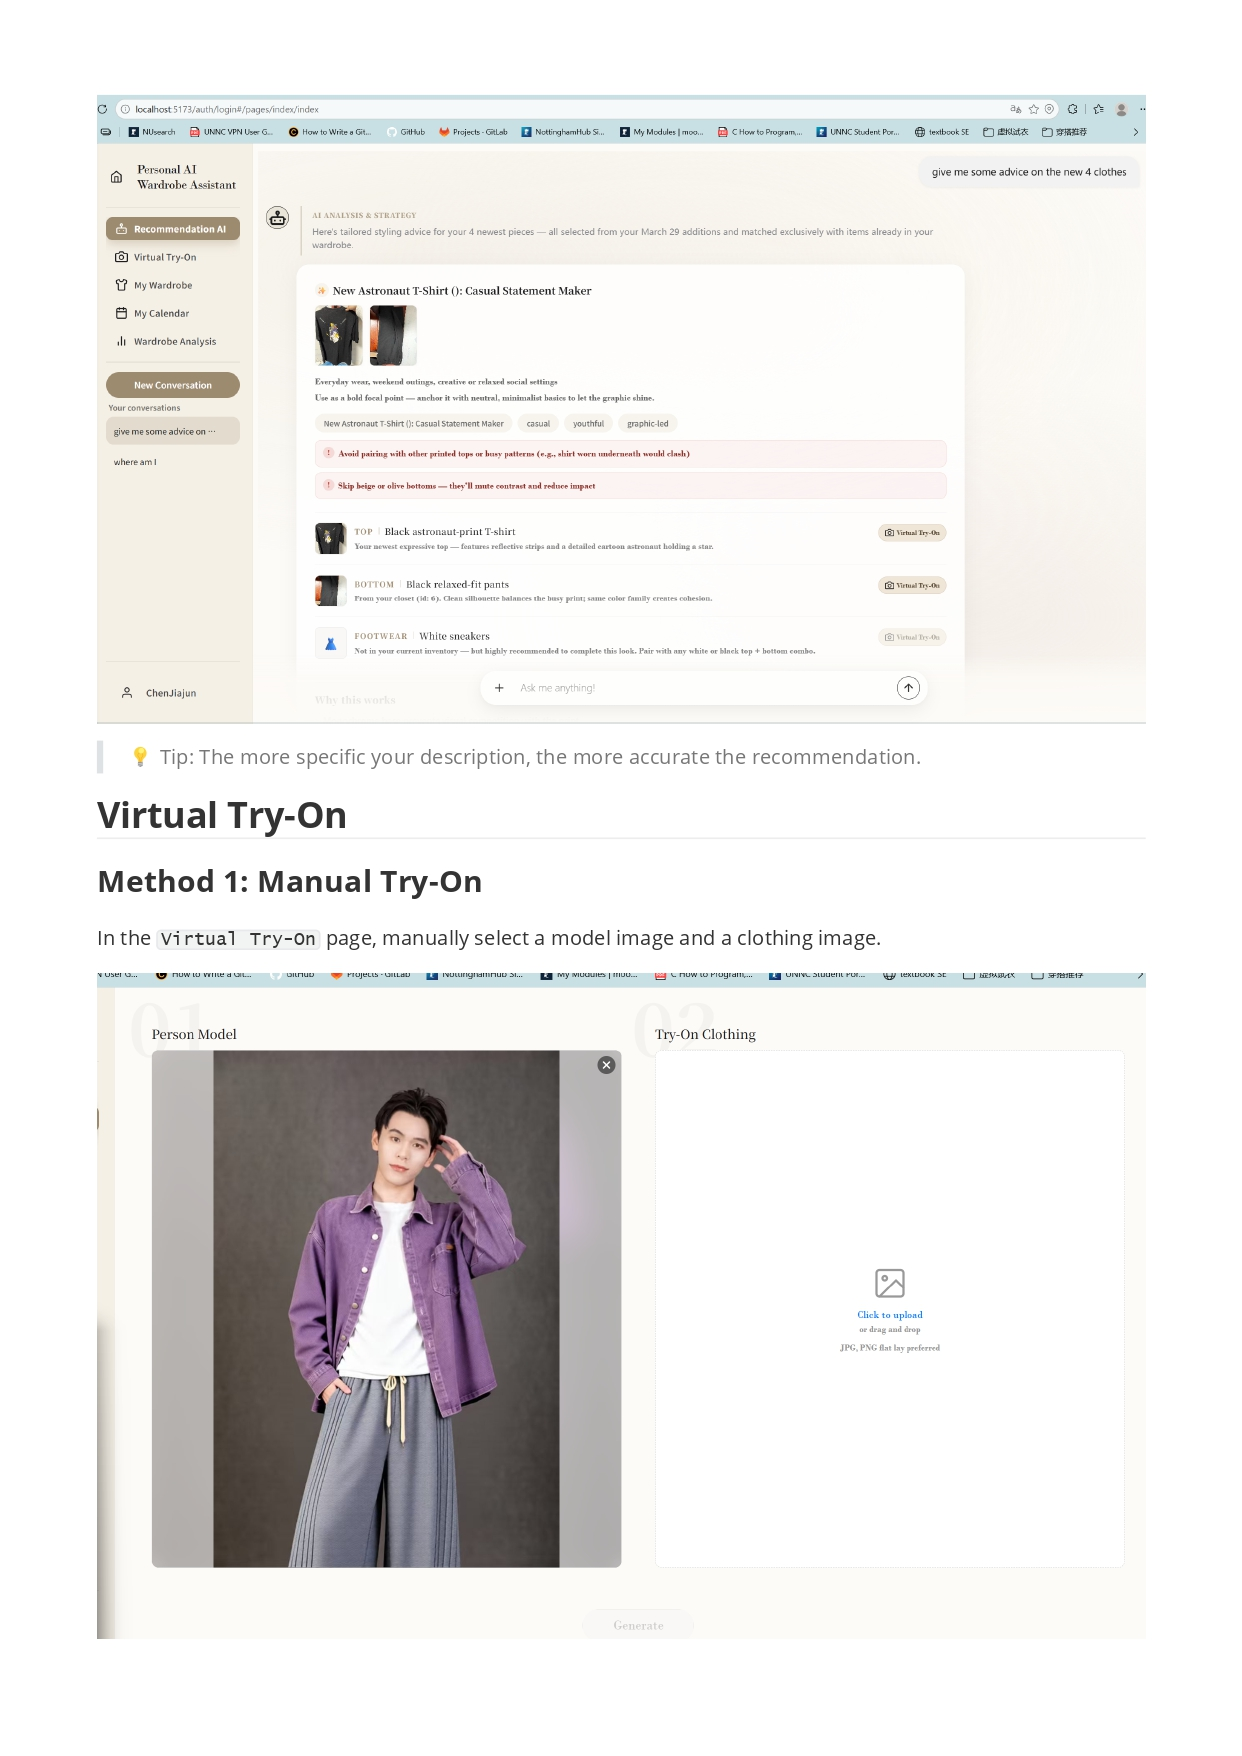
\includegraphics[width=1.0\textwidth]{images/appendix/user-manual/user_manual_page-0009.jpg}
\end{figure}
\begin{figure}[H]
    \centering
    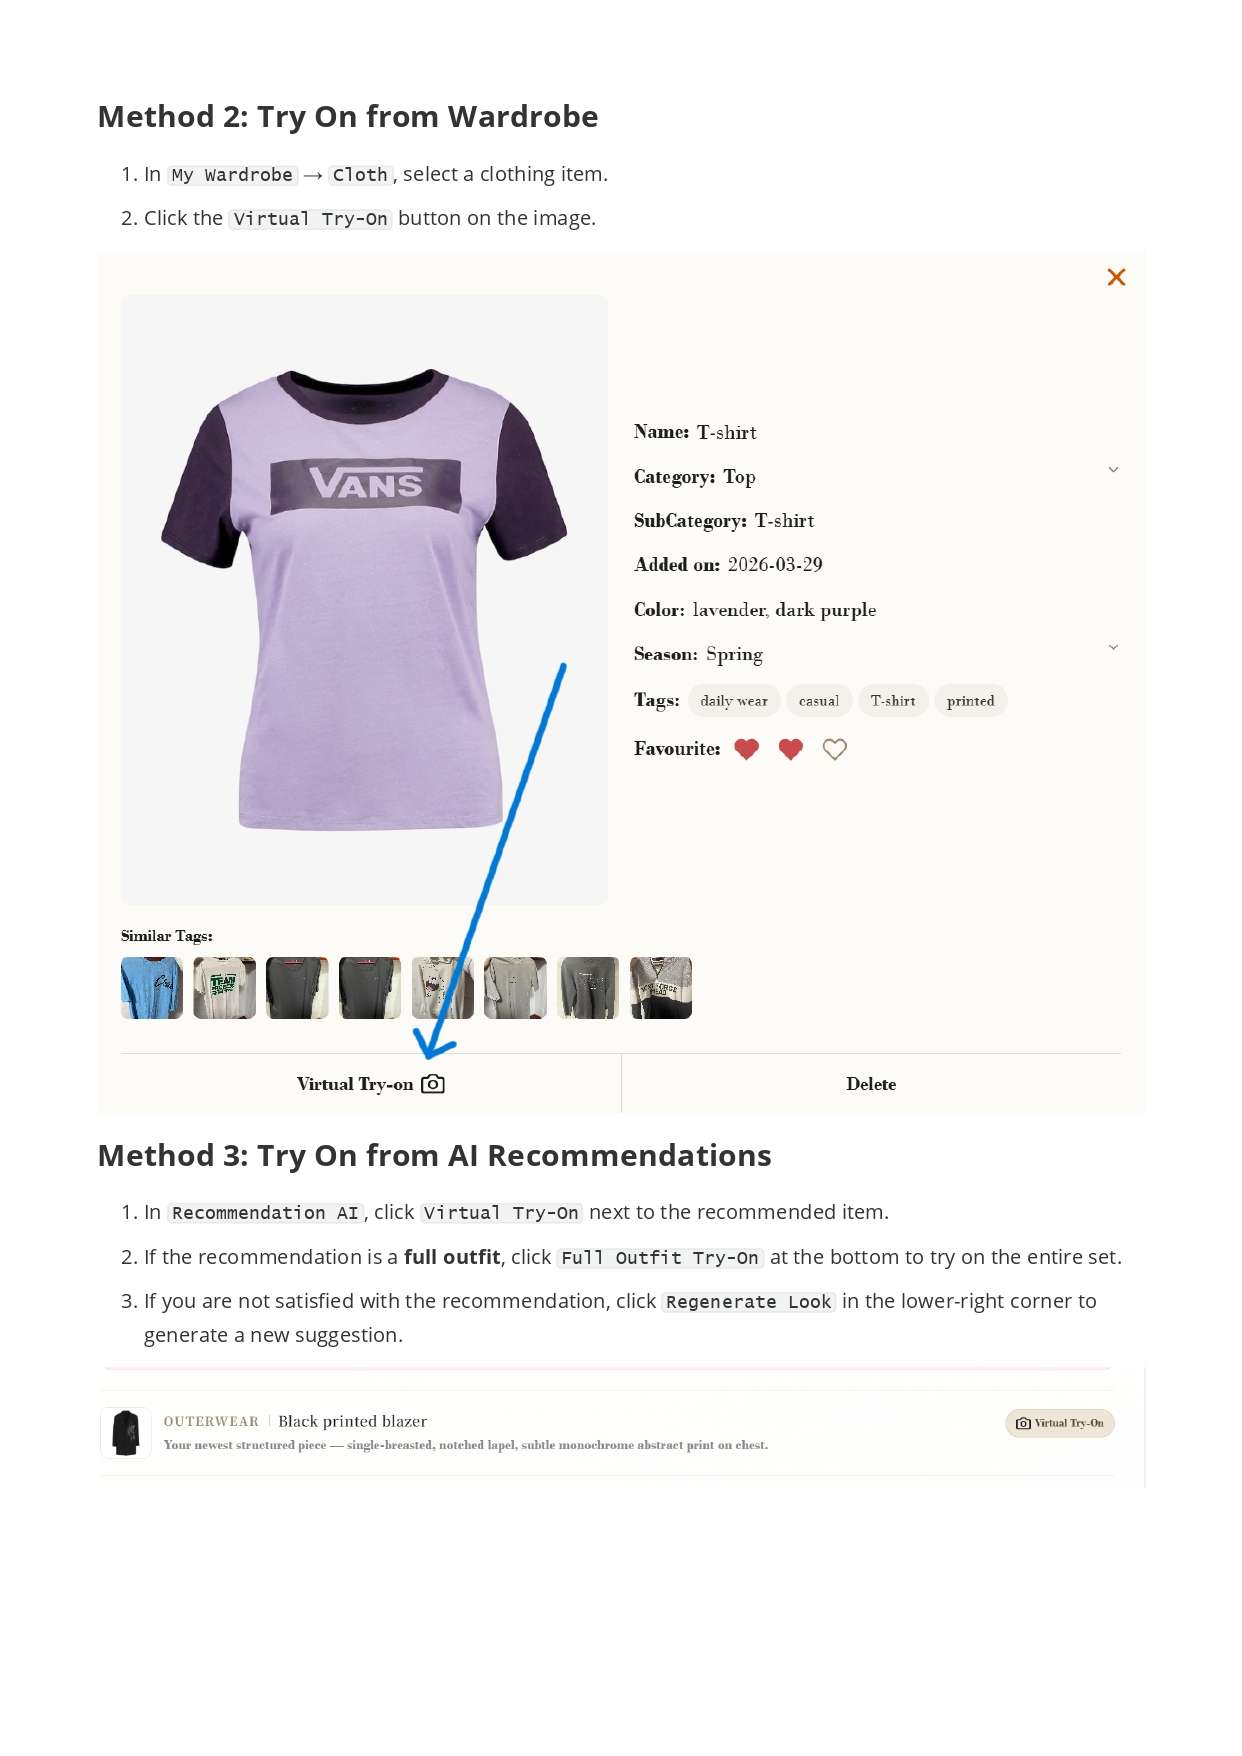
\includegraphics[width=1.0\textwidth]{images/appendix/user-manual/user_manual_page-0010.jpg}
\end{figure}
\begin{figure}[H]
    \centering
    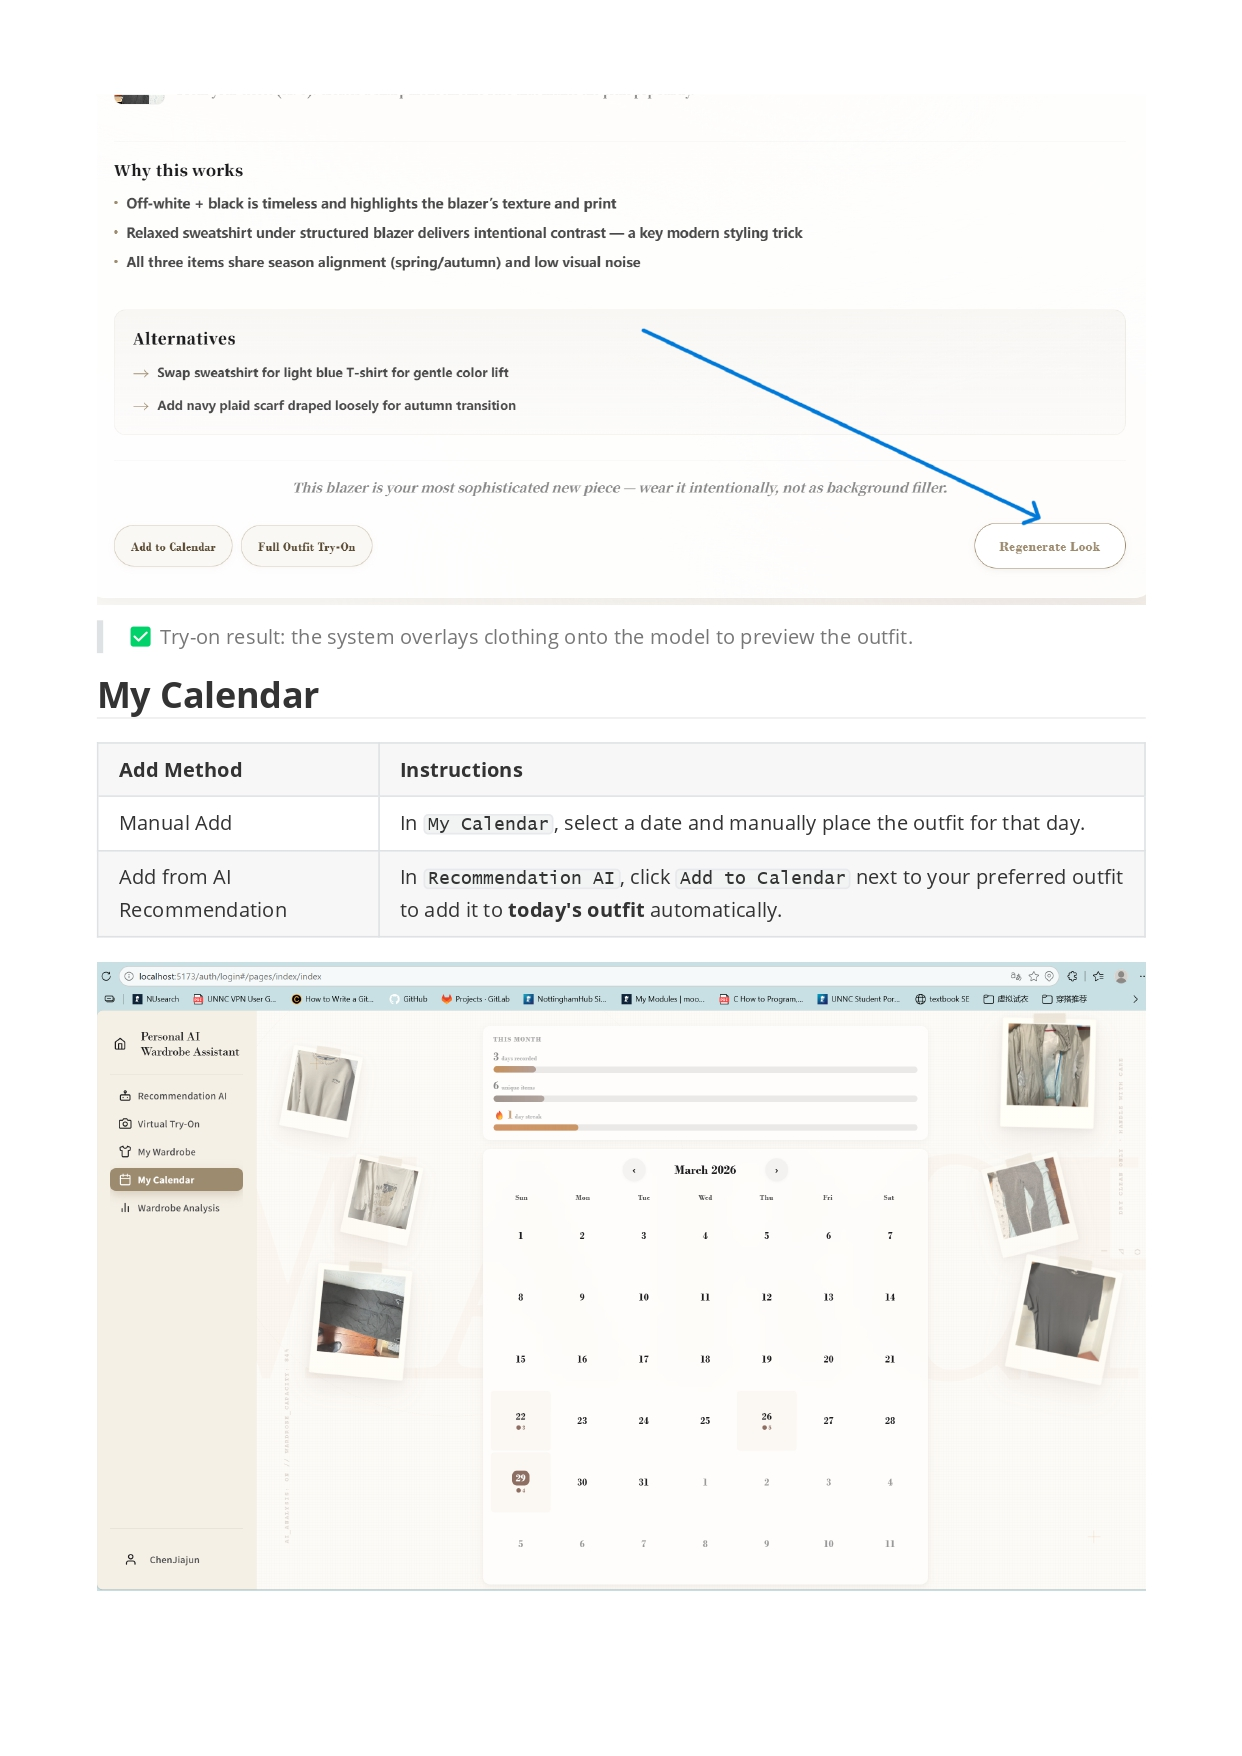
\includegraphics[width=1.0\textwidth]{images/appendix/user-manual/user_manual_page-0011.jpg}
\end{figure}
\begin{figure}[H]
    \centering
    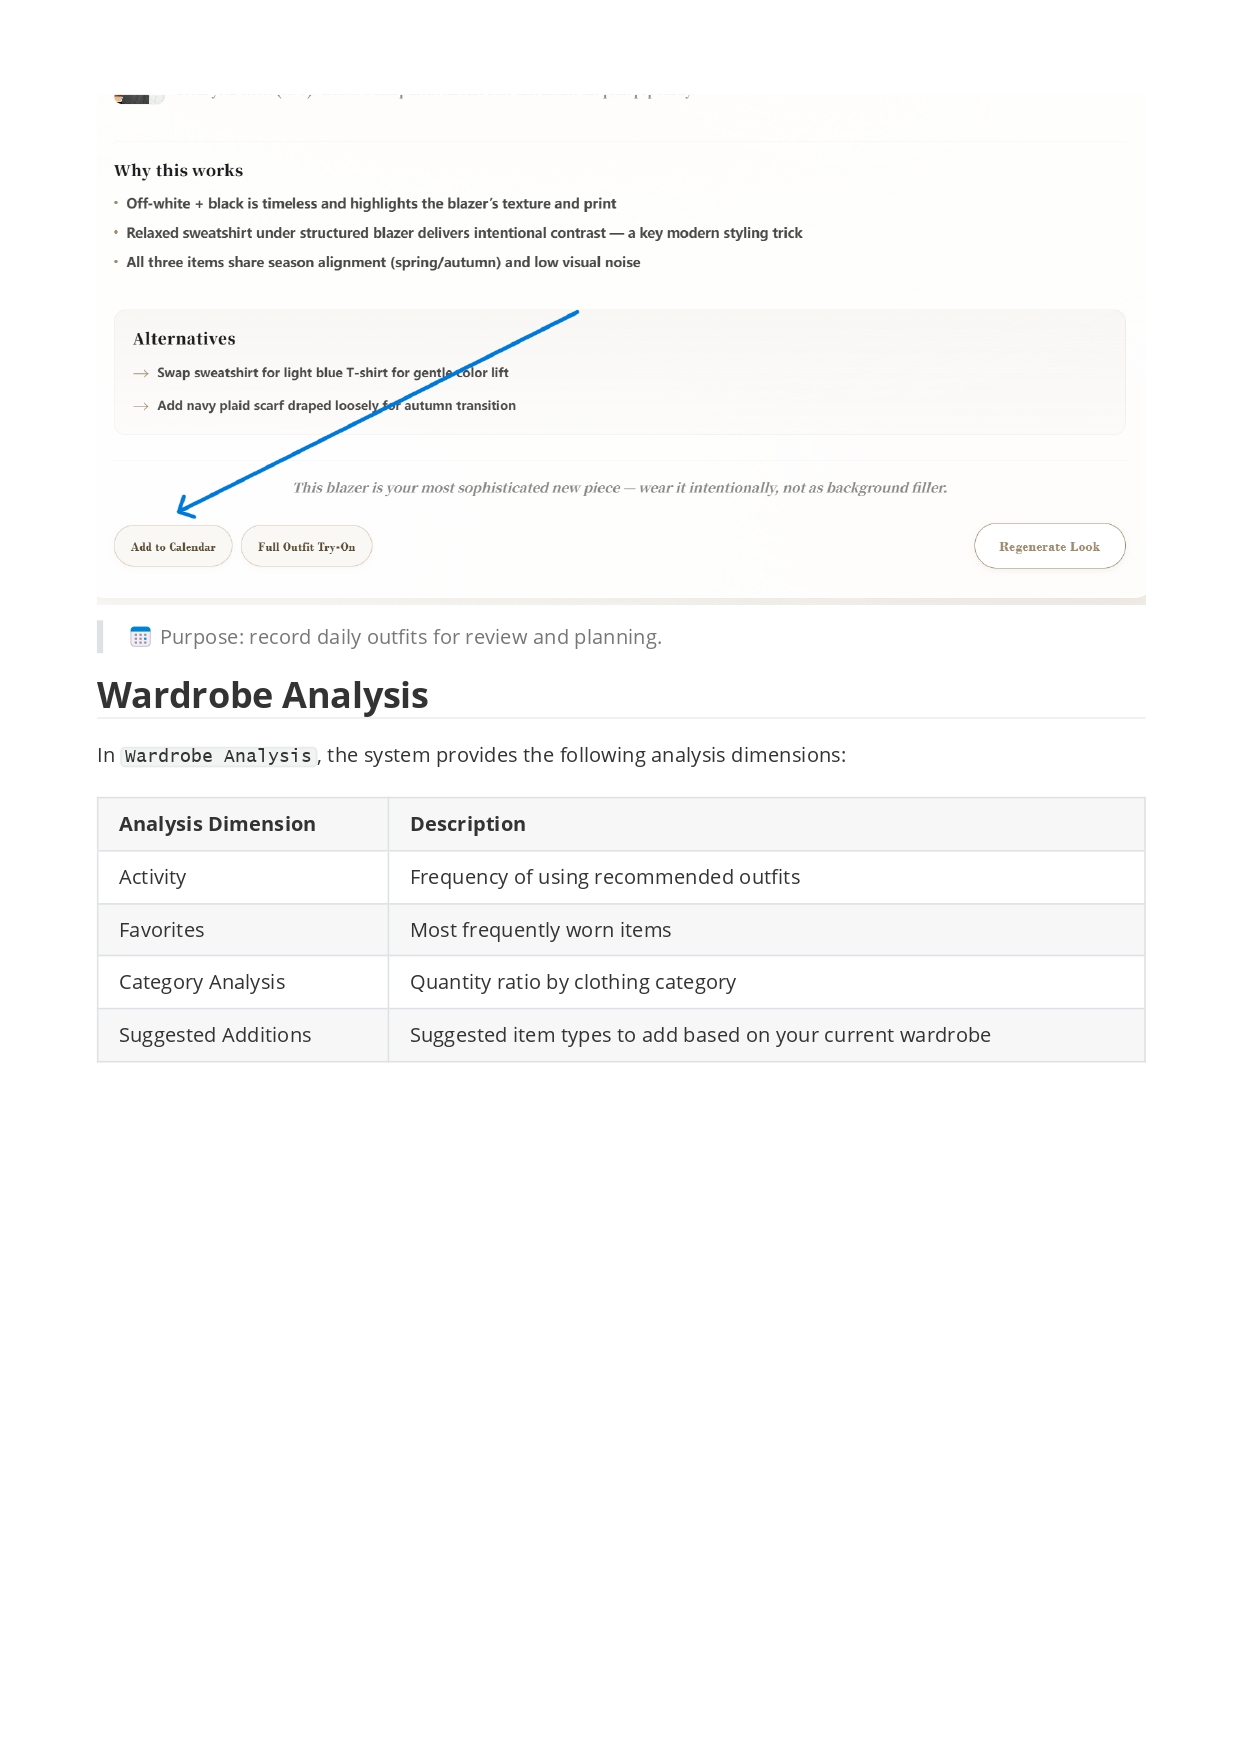
\includegraphics[width=1.0\textwidth]{images/appendix/user-manual/user_manual_page-0012.jpg}
\end{figure}
\begin{figure}[H]
    \centering
    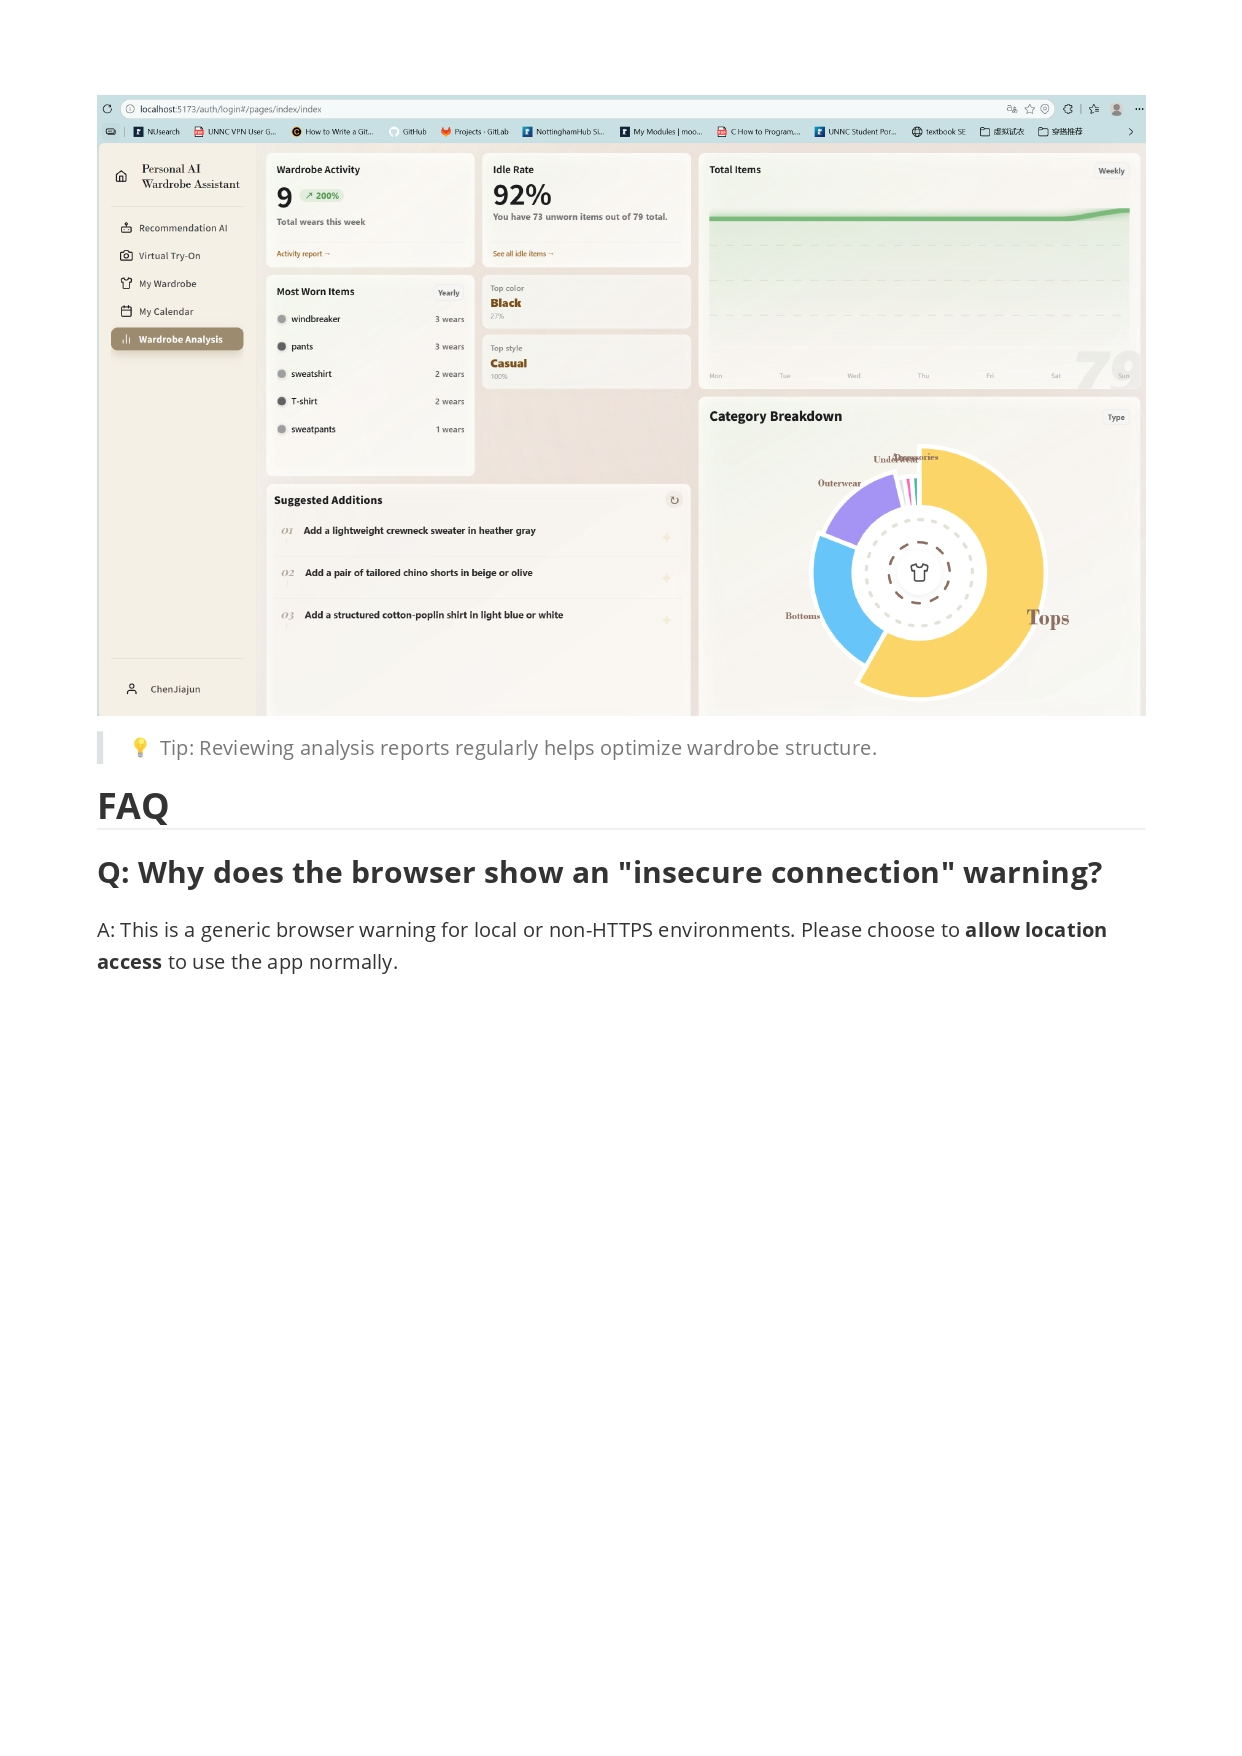
\includegraphics[width=1.0\textwidth]{images/appendix/user-manual/user_manual_page-0013.jpg}
\end{figure}
\begin{figure}[H]
    \centering
    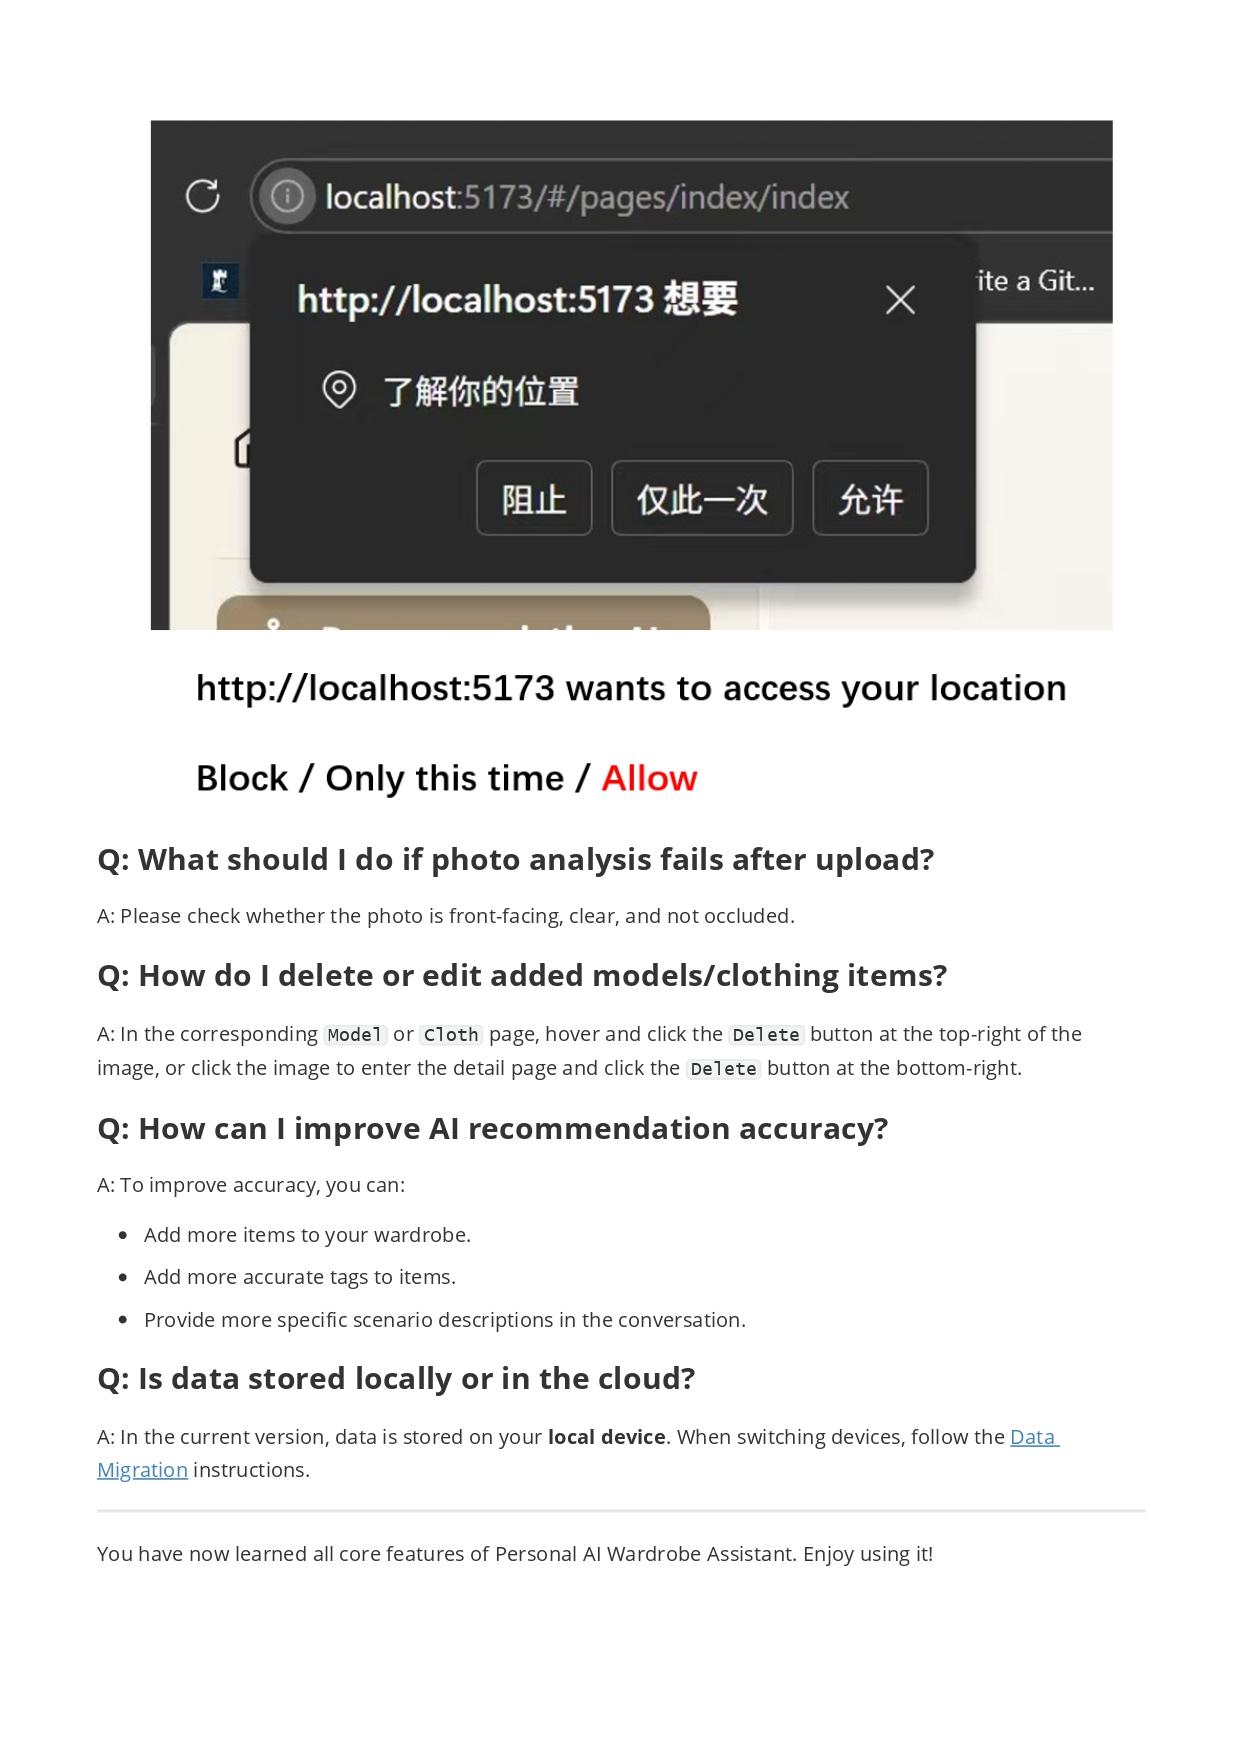
\includegraphics[width=1.0\textwidth]{images/appendix/user-manual/user_manual_page-0014.jpg}
\end{figure}

\end{appendices}